\documentclass[a4paper,twoside,UTF8]{ctexbook}


%%%%%%%%%%%%%%%%%%%%%%%%%%%%% 字 体 与 版 式 %%%%%%%%%%%%%%%%%%%%%%%%%%%%%%

\usepackage[charter]{mathdesign}
\setCJKmainfont{方正聚珍新仿简体}
\setCJKfamilyfont{hei}{FZYouHeiS}

\usepackage{geometry}
\geometry{
 a4paper,
 total={170mm,257mm},
 left=20mm,
 top=20mm,
 }
\usepackage{fancyhdr} 
\pagestyle{fancy}
\cfoot{\hei 学而思培优}
\fancyfoot[RO,LE]{\bfseries \thepage}

%%%%%%%%%%%%%%%%%%%%%%%%%%%%%%%%%%%%%%%%%%%%%%%%%%%%%%%%%%%%%%%%%%%%%%%%%%%


%%%%%%%%%%%%%%%%%%%%%%%%%%%%%    宏    包    %%%%%%%%%%%%%%%%%%%%%%%%%%%%%%

\usepackage{graphicx}
\usepackage[colorlinks=true, linkcolor=blue]{hyperref}
\usepackage{caption}
\usepackage{CJKfntef}
\usepackage{wrapfig}
\usepackage{tagging}
\usepackage{float}
\usepackage{array}
\usepackage{xcolor}
\usepackage{mdframed}
\usepackage{lmodern}
\usepackage{upgreek}
\usepackage{amsbsy}
\usepackage{amsmath}
\usepackage{eucal}
\usepackage{enumerate}
\usepackage[T1]{fontenc}
\usepackage[utf8]{inputenc}

%%%%%%%%%%%%%%%%%%%%%%%%%%%%%%%%%%%%%%%%%%%%%%%%%%%%%%%%%%%%%%%%%%%%%%%%%%%


%%%%%%%%%%%%%%%%%%%%%%%%%%%%% 命 令 与 环 境 %%%%%%%%%%%%%%%%%%%%%%%%%%%%%%

\renewcommand{\emph}[1]{{\color{red} #1}}
\renewcommand{\arraystretch}{1.5}
\newcommand{\hei}{\CJKfamily{hei}}
\newcommand{\npg}[1]{\vspace{#1}\newpage}
\newcommand{\bs}[1]{\boldsymbol{#1}}
\newcommand{\sidenote}[1]{\marginpar{#1}}
\newcommand{\pow}[1]{\times 10^{#1}}
\newcommand{\dgr}{^\circ}
\newcommand{\cdgr}{^\circ \mathrm{C}}
\newcommand{\si}[1]{\mathrm{#1}}
\newcommand{\ud}{\textrm{d}}
\newcommand{\ue}{{\rm e}}
\newcommand{\ui}{{\rm i}}
\newcommand{\ke}{\frac{1}{4\pi\varepsilon_0}}
\newcommand{\kb}{\frac{\mu_0}{4\pi}}
\newcommand{\ca}{\raisebox{0.5mm}{------}\,}
\newcommand{\dbar}{\textrm{\dj}}

%%%%%%%%%%%%%%%%%%%%%%%%%%%%%%%%%%%%%%%%%%%%%%%%%%%%%%%%%%%%%%%%%%%%%%%%%%%%


%%%%%%%%%%%%%%%%%%%%%%%%%%%%%%     正    文    %%%%%%%%%%%%%%%%%%%%%%%%%%%%%

\title{\hei \Huge 高二物理竞赛 \\ 力学}
\author{陈博}
\date{}


\begin{document}

\frontmatter
\maketitle
\usetag{teacher}

\mainmatter
\tableofcontents

%!TEX root = ../physical-olympics-2.tex
\chapter{运动学}

\section{时空与物质}

物理学,\,从刚开始成为实验性的科学的伽利略时期开始,\,到近半个世纪年来理论物理学家对额外维度的探讨,\,都给予了\emph{时空}(spacetime)最核心的地位.\,牛顿的理论,\,分析力学,\,经典场论,\,相对论这些理论最基本的图像都是时空与\emph{物质}(matter)的分立性.\,时空是装备了一个能体现出物理物理意义的\emph{度量}(metric)的3+1维对象\footnote{数学上有一套严格的说法,\,把这种连续,\,光滑的四维对象称为\emph{伪黎曼流形}(pseudo-Riemannian manifold).}.\,而物质是在每个时空点处的某种结构.\,下面会分别介绍不同物质体系的描述方法.\,在这之前我们来看看不同的时空观:

\subsection{时空观,\,坐标系}
牛顿力学理论体系基于\emph{伽利略时空观}(Galilean spacetime picture),\,也就是\emph{绝对时空观}(absolute spacetime picture).\,在这里空间是三维的平直空间.\,设想一个人站在该空间的某个空间点,\,他的胸前,\,头顶和右手平举的三个方向就是相互垂直的方向.\,如果以自己的臂长为标准长度,\,他能够定义空间中每两个点之间的空间间隔.\,事实上,\,这个人能够以一种正确的方式为每个空间点定义一个坐标,\,那么所有三维空间点的集合与任意两个点之间的距离为:
\[A(x,y,z)\in\mathbb{R}^3 \quad;\quad x,y,z\in\mathbb{R}\]
\[A(x_1,y_1,z_1)\;,\;B(x_2,y_2,z_2)\;:\;l^2=\overline{AB}^2=(x_1-x_2)^2+(y_1-y_2)^2+(z_1-z_2)^2\]

因为空间不同于时间,\,我们为以上数字赋予特殊的物理含义,\,也就是加上\emph{量纲}(dimension).\,如果两点坐标为$(0,0,0)$和$(1,1,1)$,\,那么$l=\sqrt{3}{\rm m}$,\,而不是$l=\sqrt{3}$.\,其单位${\rm m}$一方面表示了这个物理量的属性,\,另一方面指定了某个实际物理体系确定下来的固有长度大小.\,现行的(2018年1月1日,\,下文同)国际单位制对$1{\rm m}$的定义如下\footnote{一方面,\,它依赖于狭义相对论的正确性,\,目前极少理论物理工作者会质疑它.\,另一方面,\,应该要先定义下文的1s,\,再来定义1m.}:
\begin{verse}
1m是光在1/299792458\,s内在真空中行进的距离.
\end{verse}


这就是我们的\emph{三维平直空间}(3-dimensional flat space).\,注意空间点具有物理实际意义,\,它可以脱离坐标系而单独存在.\,事实上坐标系的原点可以建立在空间中的任意点处,\,朝向也可以是任意方向,\,两个空间点之间的距离$l$不会依赖于坐标系的选取,\,但两个点的坐标会因坐标系不同而改变.\,如果我们选取的坐标系总是下述使得两个相距很近的点之间的微元距离公式成立:
\[\ud l^2=\ud x^2+\ud y^2+\ud z^2\]


那么建立的坐标系就是一个\emph{笛卡尔坐标系}(Cartesian coordinate system),\,即\emph{空间直角坐标系}(3D orthogonal coordinate system).\,但是以空间直角坐标系为基础,\,我们又经常建立\emph{球坐标}(spherical coordinate)和\emph{柱坐标}(cylindrical coordinate)系统.\,通常取$x$轴为\emph{幅轴}(azimuth axis),\,点在$x-y$平面上的投影与原点的连线相对$x$轴转过的角度为$\varphi$,\,即\emph{幅角}(azimuth angle).\,而$z$轴为\emph{极轴}(polar axis),\,而点与原点连线与极轴的夹角$\theta$为\emph{极角}(polar angle).\,天文观测用球坐标就很方便,\,它是以描述的空间点到原点之间的距离$r$,\,也称\emph{矢径}(radius),\,和两个描述角位置的极角幅角来构成三个坐标$(r,\theta,\varphi)$的.\,而理论物理里也常用到的柱坐标是以$(\rho,\varphi,z)$为描述空间点的坐标,\,$\rho$是空间点到$z$轴的距离.

\begin{wrapfigure}[14]{o}[-10pt]{7cm}
\vspace{-0.4cm}
\centering
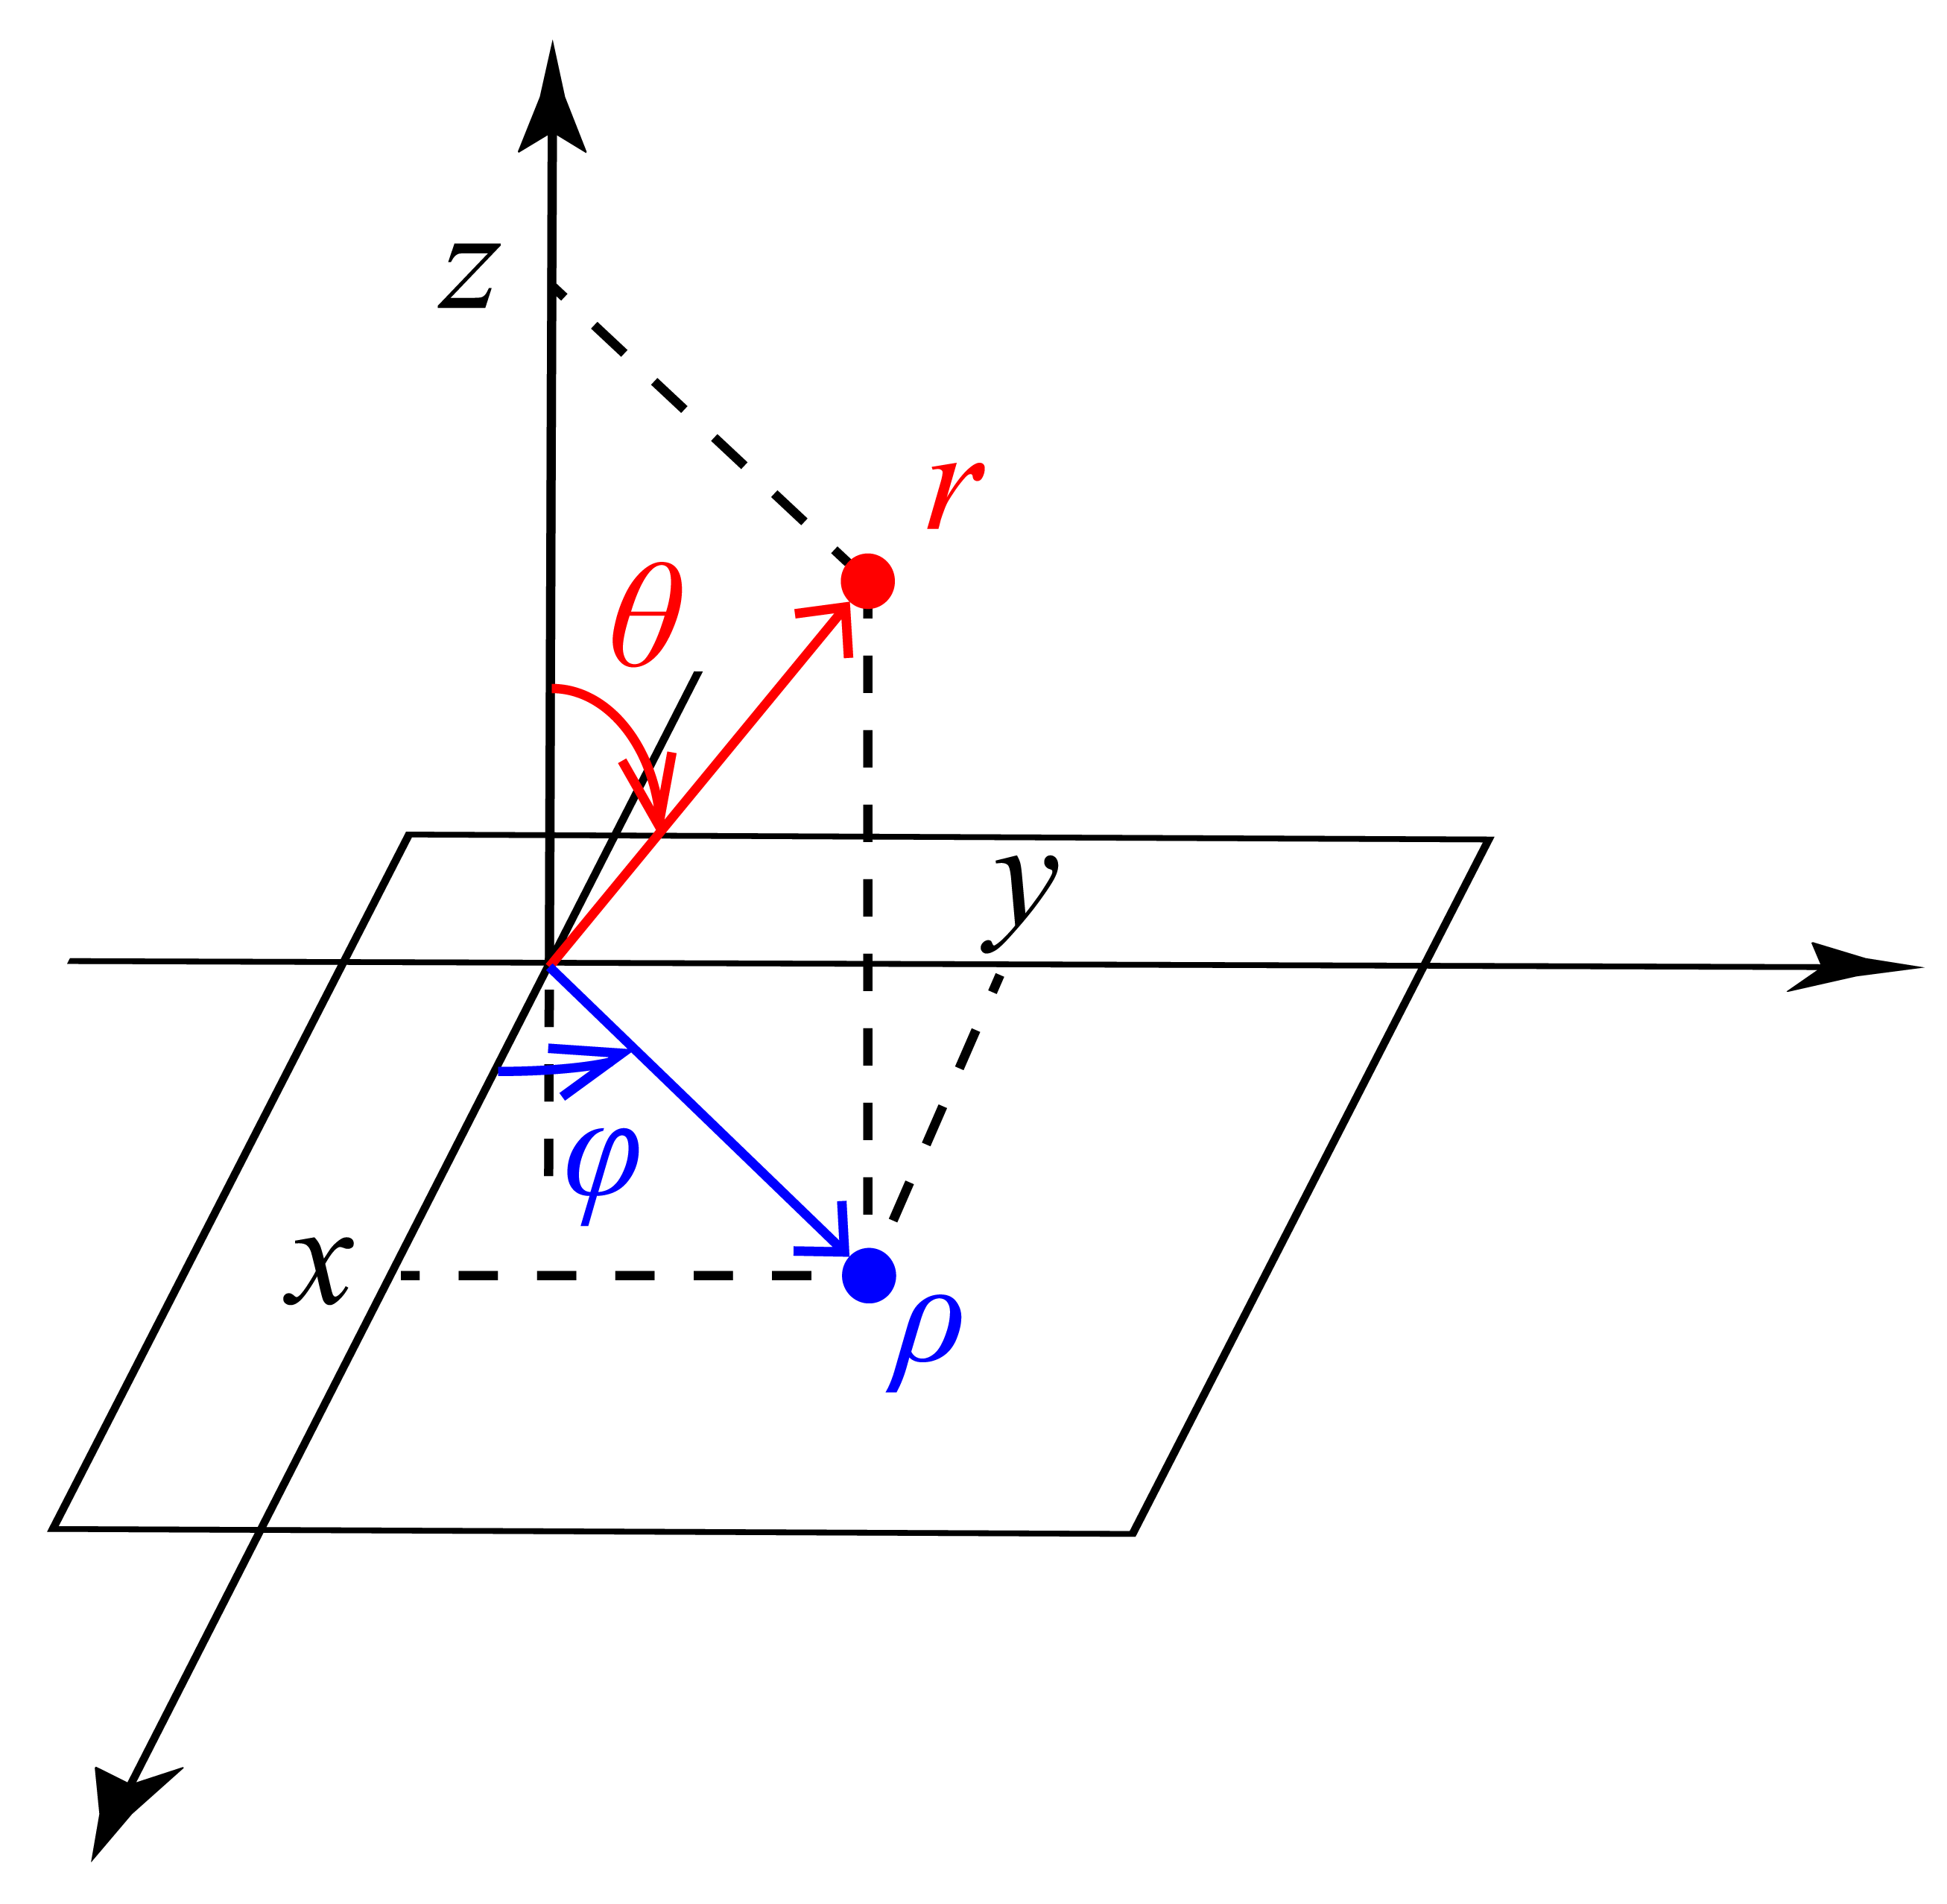
\includegraphics[width=7cm]{image/6-1-1.png}
\caption{三种坐标}
\end{wrapfigure}
需要注意,\,我们对以上$\theta,\,\varphi$角度定义比较微妙,\,$\theta$一般限制其在$[0,\pi]$范围内,\,在端点$\theta=0,\,\pi$处$\varphi$的不同取值代表同一个空间点.\,但$\varphi$的取值我们不加以任何限制,\,也就是原则上$\varphi\in\mathbb{R}$.\,而任意$\varphi$相差$2n\pi$的坐标实际上代表同一个空间点.\,这么做是因为我们最好不要用静态的几何观点去看待角度这一概念.\,而是用运动,\,变换的观点去看待角度.\,作为连续的运动的点的幅角变化也应是连续的,\,为了使点绕$z$轴一圈后幅角不至于突然改变,\,就必须默认每一点的幅角可以有多种取值,\,在具体的运动中应该灵活选择其具体取值大小.

之后经常会说到各种对称性,\,在本系列教材中我们采取如下说法:\,\emph{球对称}(spherical symmetric)仅仅代表某个函数$f(r,\theta,\varphi)$与$\varphi$无关.\,而\emph{柱对称}(cylindrical symmetric)代表的是$f(\rho,\varphi,z)$与$z$无关.\,与$\varphi$和$\theta$都无关的$f(r,\theta,\varphi)=f(r,\forall\theta,\forall\varphi)$被称为\emph{各向同性}(isotropic).\,最后\emph{中心对称}(centrosymmetric)是一个很弱的对称性,\,它仅仅代表函数在\emph{中心反演}(space inversion)下的对称性:
\[f(x,y,z)=f(-x,-y,-z)\]

绝对时空观中的时间则是一种完全与空间独立的属性.\,实际上,\,每一个空间点处的人都能感受到时间的流逝.\,十分抽象的把这些不同的时刻画在一根时间轴上,\,便是一维的时间坐标:
\[A(t)\in\mathbb{R} \quad;\quad t\in\mathbb{R}\]

而时空又是两个独立的概念.\,任意一个坐标点处都有时间轴,\,而任意一个时刻都有一个三维空间切片.\,事实上,\,我们的时空是一个3+1维的结构,\,合理地选取坐标后,\,实际上可以把时空结构写成四维坐标:
\[A(x,y,z,t)\in\mathbb{R}^4 \quad;\quad x,y,z,t\in\mathbb{R}\]

而对于任意两个时空点,\,存在绝对的时间,\,也就是可以找到两个事件的绝对时间差:
\[\tau=|t_2-t_1|\]

但空间距离却具有相对性.\,我们要求在同一时刻的同一空间切片上定义空间的度量:
\[t_1=t_2:\quad l=\sqrt{(x_1-x_2)^2+(y_1-y_2)^2+(z_1-z_2)^2}\]

不同时刻的空间,\,被线性地组织在一起,\,保证每一刻都平直的空间既不会随时间膨胀收缩,\,也不会旋转加速.\,这种时空结构被叫做\emph{牛顿-嘉当几何}(Newton-Cartan geometry)\footnote{用更为严格的语言来说,\,我们需要一个装备了一阶形式``钟''$c_\nu$和二阶逆变半正定对称张量类空间度规$s^{\mu\nu}$的四维微分流形$\mathscr{M}$:
\[\mathscr{M}:\quad s^{\mu\nu}c_{\nu}=0\]}.

时间是一个新的量纲,\,其国际单位制对$1{\rm s}$的定义为:
\begin{verse}
1s是铯-133原子基态的两个超精细能级之间跃迁所对应的辐射周期时长的9192631770倍.
\end{verse}

牛顿-嘉当几何的显著特点是物理量的定义没有所谓的\emph{协变性}(covariance).\,固然,\,在三维空间坐标框架的旋转下,\,任何物理过程中的事件所发生的位置坐标发生旋转变换,\,而几乎所有标量(比如质量,\,能量)都不变,\,几乎所有矢量(比如动量,\,角动量)都按照类似坐标变换的法则发生变换.\,但是,\,对于更普遍的一列\emph{伽利略变换}(Galilean transformation),\,也就是相对匀速运动的参考系之间的变换,\,时空坐标的形式却不能简单地推广到能量动量角动量上.

不同于绝对时空观中时间与空间成为相互独立的量纲的特点,\,狭义相对论改变了对基本物理量的看法.\,狭义相对论把时空看成为可以相互转化的不可分割的新的3+1维整体,\,同时性已然破缺.\,两个时空点之间无法定义绝对的时间间隔.\,在\emph{相对论时空观}(relativistic spacetime picture)下,\,时间和空间可以用同一把尺子去丈量:\,这是由于光速的不变性:
\[c=299792458{\rm m/s}\]

而量出来的长度叫做\emph{时空间隔}(spacetime interval):
\[\ud s^2=c^2\ud t^2-\ud x^2-\ud y^2-\ud z^2\]

这赋予时空以截然不同的结构,\,最关键的一点是,\,时间的绝对性被取消了,\,不同事件发生时间先后的比较不总是可行,\,相对论的有限速度因果律在这里取代了经典观点的时序因果律.\,我们将在 电磁学理论的最后介绍相对论理论.


\subsection{物质}

时空是物理过程发生的舞台.\,那么将物质引入后舞台上所演出的便是\emph{事件}(event).\,事件这个物理概念由这样的数学工具来描述:\,它的第一个要素自然是时空坐标$(\bs{r},t)$,\,是事件在时空上的外化.\,第二个要素是事件内禀的属性.\,它取决于所引入的物质种类,\,还取决于我们所关心问题的层次.\,一般用标量,\,矢量,\,乃至张量这样的数学工具来描述它.\,举例,\,电磁场物质在经典物理中用电场磁场来描述,\,但在\emph{量子力学}(quantum mechanics,\, QM)中这不够了,\,需要用矢势和标势来描述才是完整的.\,在更深的\emph{量子场论}(quantum field theory,\, QFT)中甚至这也是不够的.\,还需要量子化为光子才合适.\,又比如,\,电子这个很有意思的现象,\,最简单的模型是质点模型,\,内禀的属性是质量,\,动量与能量\footnote{不要认为动量能量不是内禀的而是由时空运动所决定的,\,读者可以思考在水中一个气泡的上升,\,它为体系带来的动量方向如何?}.\,然而与电磁场的经典相互作用强度告诉我们还有一项内禀属性叫做电荷量.\,近代人们惊奇地发现原来电子还固有磁矩,\,与之相应的电子具有自旋.\,最后狄拉克等人发展出\emph{量子电动力学}(quantum electrodynamics,\,QED),\,统一地用一个四分量的旋量波函数和它的方程中的若干参数来完整地描述所有发现的电子内禀属性.

\vspace{0.5cm}
\emph{经典物理学}\footnote{本书的经典物理学指牛顿力学,\,分析力学,\,经典电磁学,\,经典统计力学与狭义相对论的范畴.}(classical physics)中涉及到的物质主要有:

\vspace{0.2cm}
{\bf 1.\,质点(point mass,\,particle)}

不得不承认质点是牛顿力学的根基,\,一切可观的结论的出发点.\,质点所对应的事件集合为时空中的一条\emph{世界线}(world line).\,每一个时间仅仅有可能只有一个事件发生.\,实际上质点的运动用\emph{运动学方程}(kinematic equation)来描述:
\[\bs{r}=\bs{r}(t)=\left(x(t),y(t),z(t)\right)\]

而\emph{质量}(mass)是质点必要的内禀属性.\,它将作为参数出现在下一节介绍的动力学方程中.\,它反应物质受到同样大小的相互作用运动状态改变的难易程度.\,国际单位制从1889年至2018年末对$1\rm kg$的定义如下:

\begin{verse}
1kg是保存在法国巴黎布勒特伊宫的国际计量局实验室的约47立方厘米立式铂铱合金小圆柱的质量.\,当然,\,出于实用考虑,\,也是很多它的官方复制体的质量.
\end{verse}

这个定义今已经有一百多年了,\,历史远长于其他六个国际基本单位.\,但目前这一古老的定义方式已经被废除,\,新的定义\footnote{一方面,\,它依赖于狭义相对论和量子力学的正确性,\,目前极少理论物理工作者会质疑它.\,另一方面,\,应该要先定义上文的1s和1m,\,再来定义1kg.}为:

\begin{verse}
1kg被这样定义:\,取普朗克常数的固定数值在单位$\rm kg\cdot m^2\cdot s^{-1}$下为$\rm 6.62607015\times 10^{-34}$.
\end{verse}

长度,\,时间和质量为三大力学量纲,\,量纲是物理量的属性,\,物理量的表示方法为数值加单位,\,每个量纲有自己独特的一套单位,\,不同单位间差一个纯数的倍率.\,在物理量的加减时量纲必须相同而且结果保持量纲不变.\,但不同量纲物理量可以进行乘除而生成新的量纲.\,除了简单的加减乘除的以上规则以外,\,其他特殊函数必须只能作用在无量纲的纯数上.\,这叫做\emph{量纲法则}(dimensional rules).

\vspace{0.2cm}
{\bf 2.\,质点系(particle system)}

质点系是对质点的一种自然扩展.\,讨论质点的运动时质点受到的相互作用来自何方?\,在牛顿力学的框架下必然来自施力物体.\,故把受力物体和施力物体都作为简单的质点时,\,两个质点就可以作为整个体系讨论,\,把相互作用区分为内力与外力而推广之前的结论,\,在这个过程中我们能体会到哪些结论是一脉相承的普遍规律而哪些需要重新审视与修改.\,从原理上质点系不过是多个质点同时存在的情况而已.\,而\emph{经典统计力学}(classical statistic mechanics)是这种观点的提炼与延伸,\,它着眼于一个宏观大分子数的体系的长时间平均下的行为,\,理论上常常结合概率论的做法,\,对等概率的体系代表点构成的系综做平均.\,从中提取统计力学下不平凡的物理量.

\vspace{0.2cm}
{\bf 3.\,连续介质(continuous media)}

一方面,\,连续介质是从纯粹的理论过渡到实际问题的至关重要一步.\,另一方面,\,在处理连续介质的问题中形成了场论,\,它作为了一种与质点截然不同的物理图像形成了自己的一整套理论.\,更重要的,\,量子场论认为由于不确定原理,\,质点与世界线的观点实际上是作为场的传播的一种近似.\,也就是说,\,场论相比质点的力学更具有兼容性和普适性.\,对于简单的连续介质,\,内禀的属性由每一个点处的质量密度$\rho$和速度$\bs{v}$描述,\,这实际上形成了一个标量场和矢量场:
\[\rho=\rho(\bs{r},t) \quad;\quad \bs{v}=\bs{v}(\bs{r},t)\]

而动力学方程的列法又强烈依赖于介质内的相互作用.\,于是这个大的问题又分出很有代表性的弹性力学和流体力学,\,还有介于两者之间的粘弹性塑性模型等等.\,还有从热力学平衡态出发考虑的近平衡态统计力学方法.

\vspace{0.2cm}
{\bf 4.\,场(field)}

\begin{wrapfigure}[16]{o}[-10pt]{7cm}
\vspace{-0.4cm}
\centering
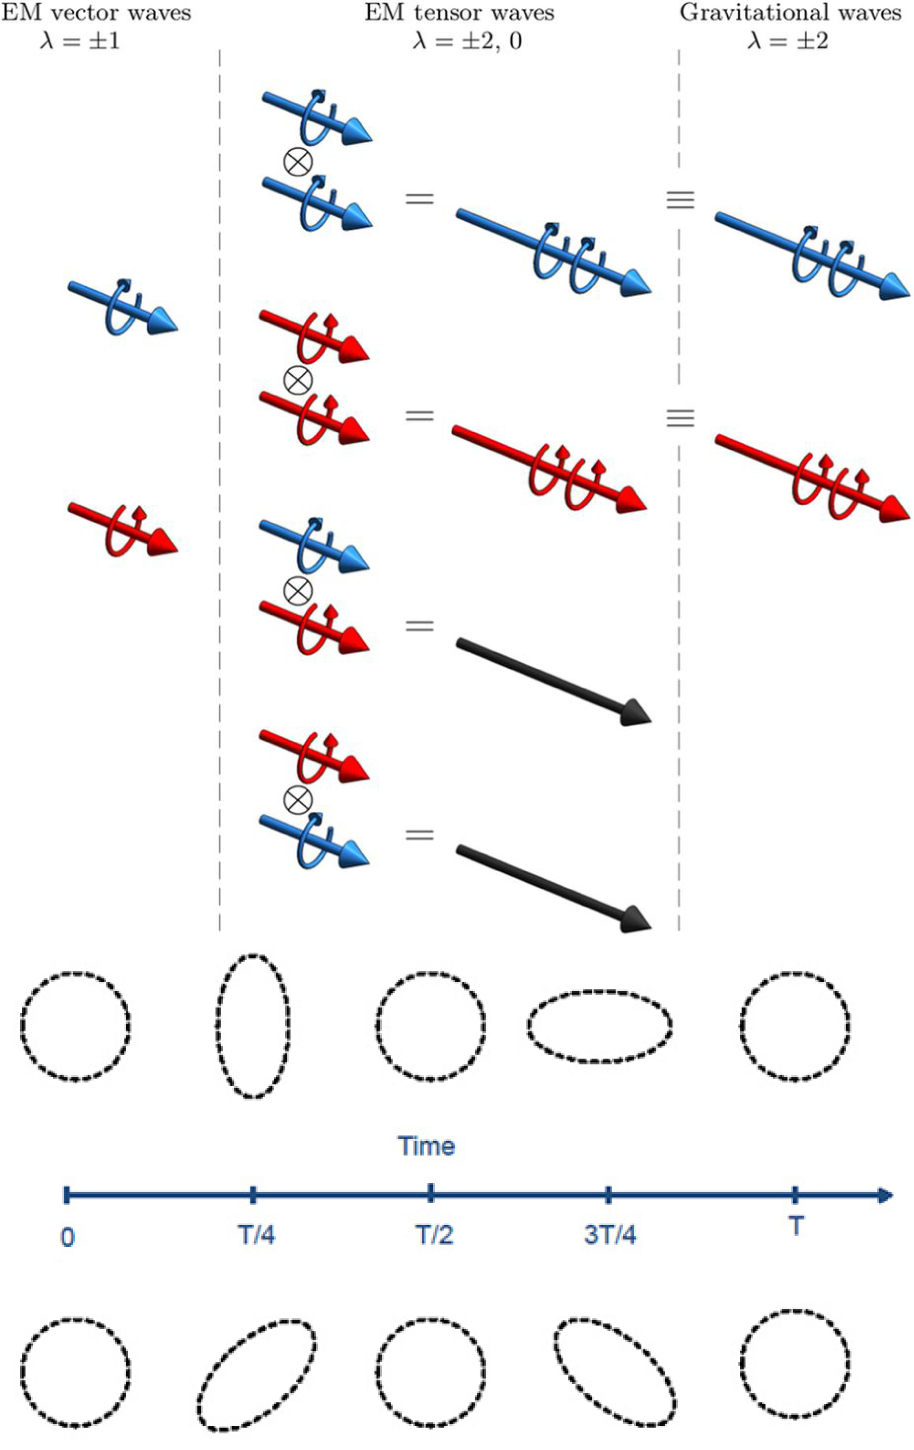
\includegraphics[width=5cm]{image/6-1-2.png}
\caption{引力波与电磁波的区别}
\end{wrapfigure}
关于场的理解历史上经历了两个过程.\,第一个阶段是正如上面的连续介质的做法,\,场是作为某种事先已经被研究的足够清楚的粒子体系与它们之间的相互作用的描述方法与数学工具.\,而从牛顿时代开始人们就默认了超距作用的存在,\,而场数学工具的第二个作用就是描述电荷之间,\,质量之间的超距作用.\,但是逐渐人们意识到相互作用传播速度的有限性,\,于是场开始变成某种与物质其他耦合的物质而单独存在,\,这就是第二阶段,\,人们意识到了场本身就是一种物质,\,电子与电子之间不能直接相互作用,\,电子改变了真空,\,稳定地与电磁场相互作用而产生库仑场,\,然后在对第二个电子产生相互作用力.\,将场作为某种先验地存在于时空中的物质形式进行描述与研究的学科就叫做\emph{场论}(field theory).\,有哪些可能的场形式?\,场的物理量如何书写?\,场与粒子,\,场与场之间如何相互作用便是场论的研究内容.\,比如说,\,动力学所关心的内容,\,场的质量本身没有定义,\,可以定义的一般是场的定域动量与波矢,\,能量与角频率,\,平面波的色散关系等等.\,的确,\,场论最基本的做法是傅里叶分解,\,它认为平面波是不受任何相互作用时的场的惯性运动方式,\,而任何场的运动,\,每一时刻都可以分解成一系列平面波的叠加.\,就好像任何复杂体系的运动本质上都是质点系的运动,\,而质点的运动每时每刻都可以看出匀速运动那样.


场论根据其描述方法分为标量场论,\,矢量场论,\,张量场论和旋量场论等.\,电磁场论是矢量场论,\,它用四势矢量$(\varphi,\bs{A})$来描述.\,引力场论在广义相对论弱场近似下是张量场论,\,但传播的引力波和电磁波类似只能有两种偏振,\,其模式为$+$型和$\times$型,\,这又是不同于电磁波的.\,在更现代的观点中,\,场是真空的某种激发,\,十分类似于一张二维的拉紧的薄膜,\,没有任何振动时它已经固有能量了,\,场物质反应为膜的各种振动形式.\,而一个石子受到外力而压弯了膜,\,就可以理解为粒子与场之间的相互作用.



\subsection{参考系,\,物理规律与其不变性}

\emph{坐标系}(coordinate system)是一套用来描述时空点位置的坐标系统,\,而\emph{参考系}(reference system)则是下文将引申的一类坐标系的统称.

在伽利略时空观\footnote{本章仅限讨论非相对论,\,相对论见后}下参考系的定义相对简单.\,我们只需要任意指定一个观察者,\,观察者可以在$3+1$维的时空中作任意运动,\,每一个时刻对应一个测量的坐标系统:\,观察者分别以右手边,\,胸前和头顶三个方向建立坐标系,\,坐标系的刻度就是其代表的位置到原点观察者处的空间距离.\,这样便可以表示任意事件的时空坐标.\,而且构成一个三维空间直角坐标系.\,叫做观察者的\emph{固有参考系}(proper reference system).

物理规律的本质是什么?\,在一个特定的参考系中,\,我们进行一些物理量的测量,\,测量得到的值之间在特定的实验条件下会满足特定的关系而不依赖于某些具体的参数,\,一般都是等式.\,这样的普遍成立的等式就可以反映某些物理规律.\,从\emph{动理学}(kinetics)的角度理解,\,体系的演化是\emph{状态}(state)随时间的演化,\,而体系的状态由一组完备的\emph{态参量}(state variable)描述,\,态参量可以包含一些广义坐标$q_\alpha$和他们对时间的导数即广义速度$v_\alpha=\dot{q}_\alpha$.\,而以下\emph{决定论}(determinism)则对物理规律的形式做出了规定:
\begin{quote}
动理学系统:

已知某时刻$t=0$的初态$\{q_\alpha(0),\,\dot{q}_\alpha(0)\}$后,\,应能预言任意将来的状态$\{q_\alpha(t),\,\dot{q}_\alpha(t)\}$.
\end{quote}

事实上,\,不光是将来的状态,\,在一般经典物理的框架下,\,过去的状态也是可以被``预言''的.\,这是因为我们进一步要求动理学系统的规律是以下形式的二阶方程:
\[f_i(\ddot{q}_\alpha,\,\dot{q}_\alpha,\,{q}_\alpha,\,t)=0\]

而且广义坐标的个数应该和方程的数目一致,\,方程是至多二阶的.\,微分方程的描述在数学上完全导致了体系彻底的决定性,\,只要知道初始条件便可以往前往后推理所有发生的物理现象\footnote{更有甚者,\,经典物理也难以解释耗散现象,\,在忽略耗散时,\,方程应该还具有平移对称性(不显含t)和时间反演对称性(方程对广义速度是偶函数).\,此时对将来和对过去的预言在广义速度取相反数时是完全对称的,\,而且预言只依赖于时间差不依赖于初始时刻.}.

这一物理学科研究范围内的有关决定性的原理很强大,\,强大到历史上很多物理学家和哲学家都质疑过它的真实性和适用性.\,最著名的莫过于拉普拉斯提出的\emph{拉普拉斯妖}(Laplace's demon)的论点:\,如果存在一个全知的拉普拉斯妖,\,能够知道在某一时刻宇宙中所有原子的精确位置与动量,\,那么任意时刻的状态也能被预言.\,这种决定论观点总是被拿来与\emph{自由意志论}(free will)去归谬,\,如果过去与未来都已经被谱写,\,那么人类所有的行为的意义和动机也就不能被解释.\,这直到今天也是科学与哲学未能获得满意的回答的问题.

但是科学的一个目的就是在于能够对未发生的事情进行预言,\,所以本着对决定论的认可与尊重,\,我们才能继续我们的科学研究.

\vspace{1cm}

除了需要符合决定性原理,\,物理规律还需要反映出一定的对称性.\,整个牛顿的\emph{经典力学}(classical mechanics)体系都要遵从的一个大的对称性,\,我们可以称之为\emph{伽利略对称性}(Galilean symmetry),\,也是伽利略时空观的一个重要组成部分.\,这个对称性的含义如下阐释:

首先我们重拾``绝对时空观''的说法.\,其含义是存在一个特殊的观察者,\,它建立的坐标系$O-xyz$(对位于原点的观察者来说,\,是参考系)是默认的第一个使得我们以上提出的物理规律成立的坐标系.\,自身具有$3+1$维的结构:
\[(x,\,y,\,z,\,t)\in \mathbb{R}^3\times \mathbb{R}\quad,\quad \ud l^2=\ud x^2+\ud y^2+\ud z^2\]

\begin{figure}[H]
\centering
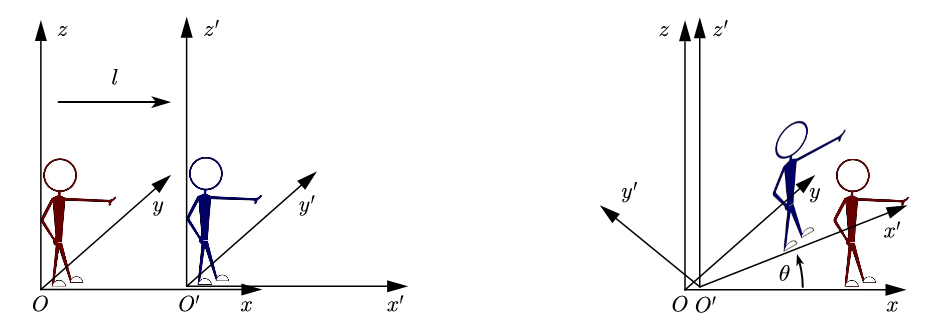
\includegraphics[width=12cm]{image/6-1-15.png}
\caption{固定平移与转动}
\end{figure}

让我们来阐明参考系与坐标系之间的区别.\,我们设想另外一个观察者,\,它与原观察者保持相对静止.\,但是其建立的坐标系$O'-x'y'z'$依然可能有很多种可能性:\,默认观察者自己为原点,\,右手边为$x$轴,\,胸前为$y$轴,\,头顶为$z$轴.\,一种可能性是,\,新观察者相对原来的观察者仅仅是做时空\emph{平移}(translation),\,而其轴的方向保持平行.\,






\section{运动的描述}

\subsection{质点的运动}
质点的运动是复杂的连续体的运动的基础.\,所谓\emph{运动}(motion)就是每一个时间都有一个位置.\,就是说位置是时间的函数:
\[\bs{r}=\bs{r}(t)\]

我们使用实数上的矢量空间和矢量来刻画真实的物理学上的二维或三维空间和其中的点.\,也即:
\[\bs{r}\in\mathbb{R}^2 \;{\rm or}\; \mathbb{R}^3\]

\begin{wrapfigure}[16]{o}[-10pt]{7cm}\label{6-1-3}
\vspace{-0.4cm}
\centering
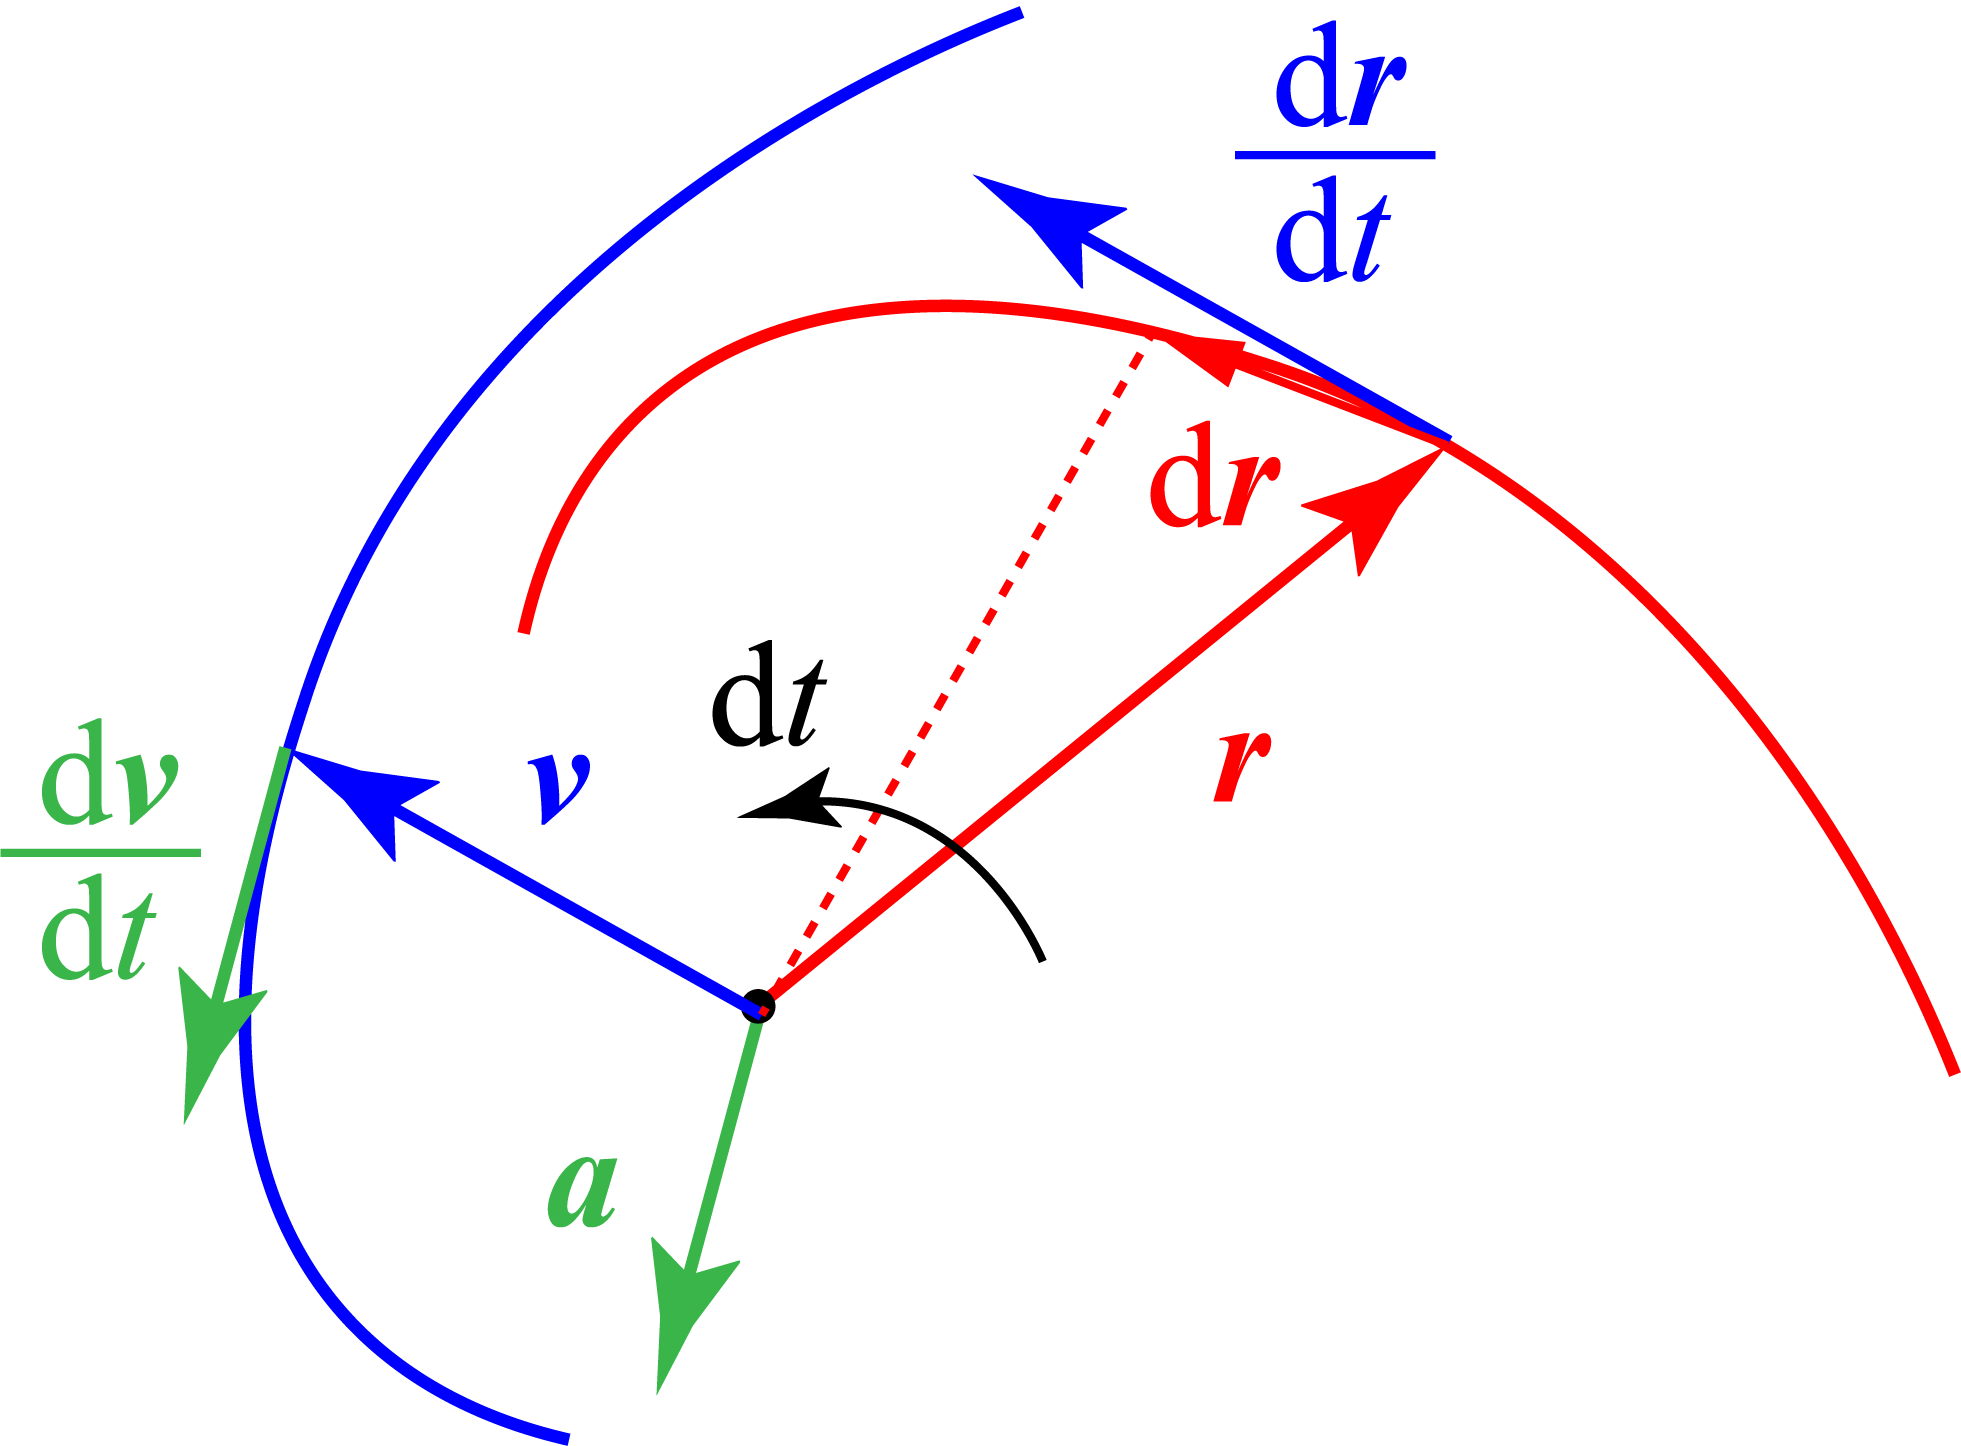
\includegraphics[width=7cm]{image/6-1-3.png}
\caption{质点的位置,\,速度与加速度}
\end{wrapfigure}
前者对应二维运动,\,后者对应三维运动.\,我们从中可以发现,\,函数是描述运动的数学工具,\,对矢量与函数的分析学知识便是运动学和物理学的基础.\,而运动学本身是可以看成是数学的一个分支的.\,对质点的位置矢量求导数便得到速度矢量,\,再求导数或是求二阶导数便是加速度矢量:
\[\bs{v}=\frac{\ud \bs{r}}{\ud t}=\lim_{\Delta t\to 0 }\frac{\bs{r}(t+\Delta t)-\bs{r}(t)}{\Delta t}\]
\[\bs{a}=\frac{\ud \bs{v}}{\ud t}=\lim_{\Delta t\to 0 }\frac{\bs{v}(t+\Delta t)-\bs{v}(t)}{\Delta t}\]
\[\bs{a}=\frac{\ud ^2\bs{r}}{\ud t^2}=\lim_{\Delta t\to 0 }\frac{[\bs{r}(t+\Delta t)-\bs{r}(t)]-[\bs{r}(t)-\bs{r}(t-\Delta t)]}{\Delta t^2}\]

正如上图\ref{6-1-3}所示,\,我们可以把每一个瞬时的速度矢量共起点画出来,\,并把端点连做曲线,\,此时背景的空间往往叫做\emph{速度空间}(velocity space),\,它的更普遍的对应是动量空间,\,这在近代物理的理论值具有重要地位.\,引入速度空间后质点的运动便可以等价地在速度空间中进行研究.\,比如在均匀重力场中的抛体运动在速度空间中就是简单的竖直向下的匀速直线运动.\,而平方反比力下的天体运动(开普勒问题)实际上在速度空间中可以证明将变为变速偏心圆周运动.\,这使得通过速度求加速度就好像通过位置求速度那样方便.\,具体求法接下来还得进一步展开.

加速度的导数偶尔也会进入物理研究的视野,\,它被叫做\emph{急动度}(jerk).\,即:
\[\bs{j}=\frac{\ud \bs{a}}{\ud t}=\frac{\ud ^3\bs{r}}{\ud t^3}\]

矢量函数概念就是实数到矢量的映射,\,但是具体能写出函数形式的例子在物理中却不是那么常见.\,比如抛体运动的运动对应的函数,\,即\emph{运动方程}(equation of motion)\footnote{指运动学运动方程,\,动力学运动方程就是反应运动的规律的,\,能够最终解出来运动学运动方程的微分方程.}为:
\[\bs{r}=\bs{r}_0+\bs{v}_0 t+\frac{1}{2}\bs{g}t^2\]

它是牛顿定律下以下微分方程结论的解:
\[\bs{a}=\frac{\ud ^2\bs{r}}{\ud t^2}=\bs{g}\]

但是在一般情况下,\,要表示出一个既有大小又有方向的矢量函数,\,我们得采用分解的思想,\,研究能够完全确定这个矢量值的参数.\,通常有以下做法:

\vspace{0.2cm}
{\bf 1.\,直角坐标系下的分解}

在一个欧几里得空间里的一个参考系中研究问题,\,很常见的一种做法是建立直角坐标系来表示一个点的位置.\,以更普遍的三维运动为例.\,既然物体的位置由坐标$(x,\,y,\,z)$来表示.\,我们就能认为表示运动的任务由三个标量函数$x(t),\,y(t),\,z(t)$来承担.\,其实这与上面介绍的用矢量来表示位置是非常一致的,\,因为实际上点的坐标通常也被理解为原点指向这个点的矢量在三个基矢的坐标:
\[\bs{r}=(x,\,y,\,z)=x\bs{i}+y\bs{j}+z\bs{k}\]

出于哈密顿(Hamilton)爵士关于把三维空间三个方向基矢视作四元数代数运算的旋转等效的奇妙观点,\,我们分别把$x,\,y,\,z$方向的基矢按照惯例记做$\bs{i},\,\bs{j},\,\bs{k}$.\,也常常因为它们是单位矢量(长度为1),\,而记做$\bs{e}_x,\,\bs{e}_y,\,\bs{e}_z$.\,这样便能把$\bs{r}$分解出$x$,\,$y$,\,$z$来.

分解以后,\,重新合成便能得到需要的物理量.\,这其中的意思是:\,比如我们为了求一个曲线运动速度或者加速度的$x$分量.\,也就是求下列表达式:
\[\bs{v}=v_x\bs{i}+v_y\bs{j}+v_x\bs{k}=\frac{\ud \bs{r}}{\ud t}\]
\[\bs{a}=a_x\bs{i}+a_y\bs{j}+a_x\bs{k}=\frac{\ud^2 \bs{r}}{\ud t^2}\]

中的分量$v_x,\,a_x$.\,其求法非常直接,\,便是:
\[v_x=\frac{\ud }{\ud t}x(t)\quad,\quad a_x=\frac{\ud^2 }{\ud t^2}x(t)\]

这相当于是说,\,求导数和向某固定方向投影是可以交换前后次序的:

\[\bs{i}\cdot \frac{\ud }{\ud t}\bs{r}=\frac{\ud }{\ud t}(\bs{i}\cdot \bs{r})\quad,\quad \bs{i}\cdot \frac{\ud }{\ud t}\bs{v}=\frac{\ud }{\ud t}(\bs{i}\cdot \bs{v})\]

这是当然的,\,因为矢量点乘的导数的法则也符合与标量乘积求导数类似的莱布尼茨法则,\,而常矢量$\bs{i}$不随着运动改变.\,所以导数只有对$\bs{r},\,\bs{v}$求导的项.

在数学上,\,曲线段也经常被描述为是与某实数上区间\emph{同胚}(homeomorphic)的几何图形,\,这其实就是说,\,存在自变量$t$,\,不失一般性地,\,我们让其取值范围为$(-\infty,\,+\infty)$.\,而存在一个从这个自变量到三维空间点$(x,\,y,\,z)$的光滑映射:
\[x=x(t)\quad ,\quad y=y(t)\quad ,\quad z=z(t)\]

\begin{wrapfigure}[10]{o}[-10pt]{7cm}\label{6-1-4}
\vspace{-0.4cm}
\centering
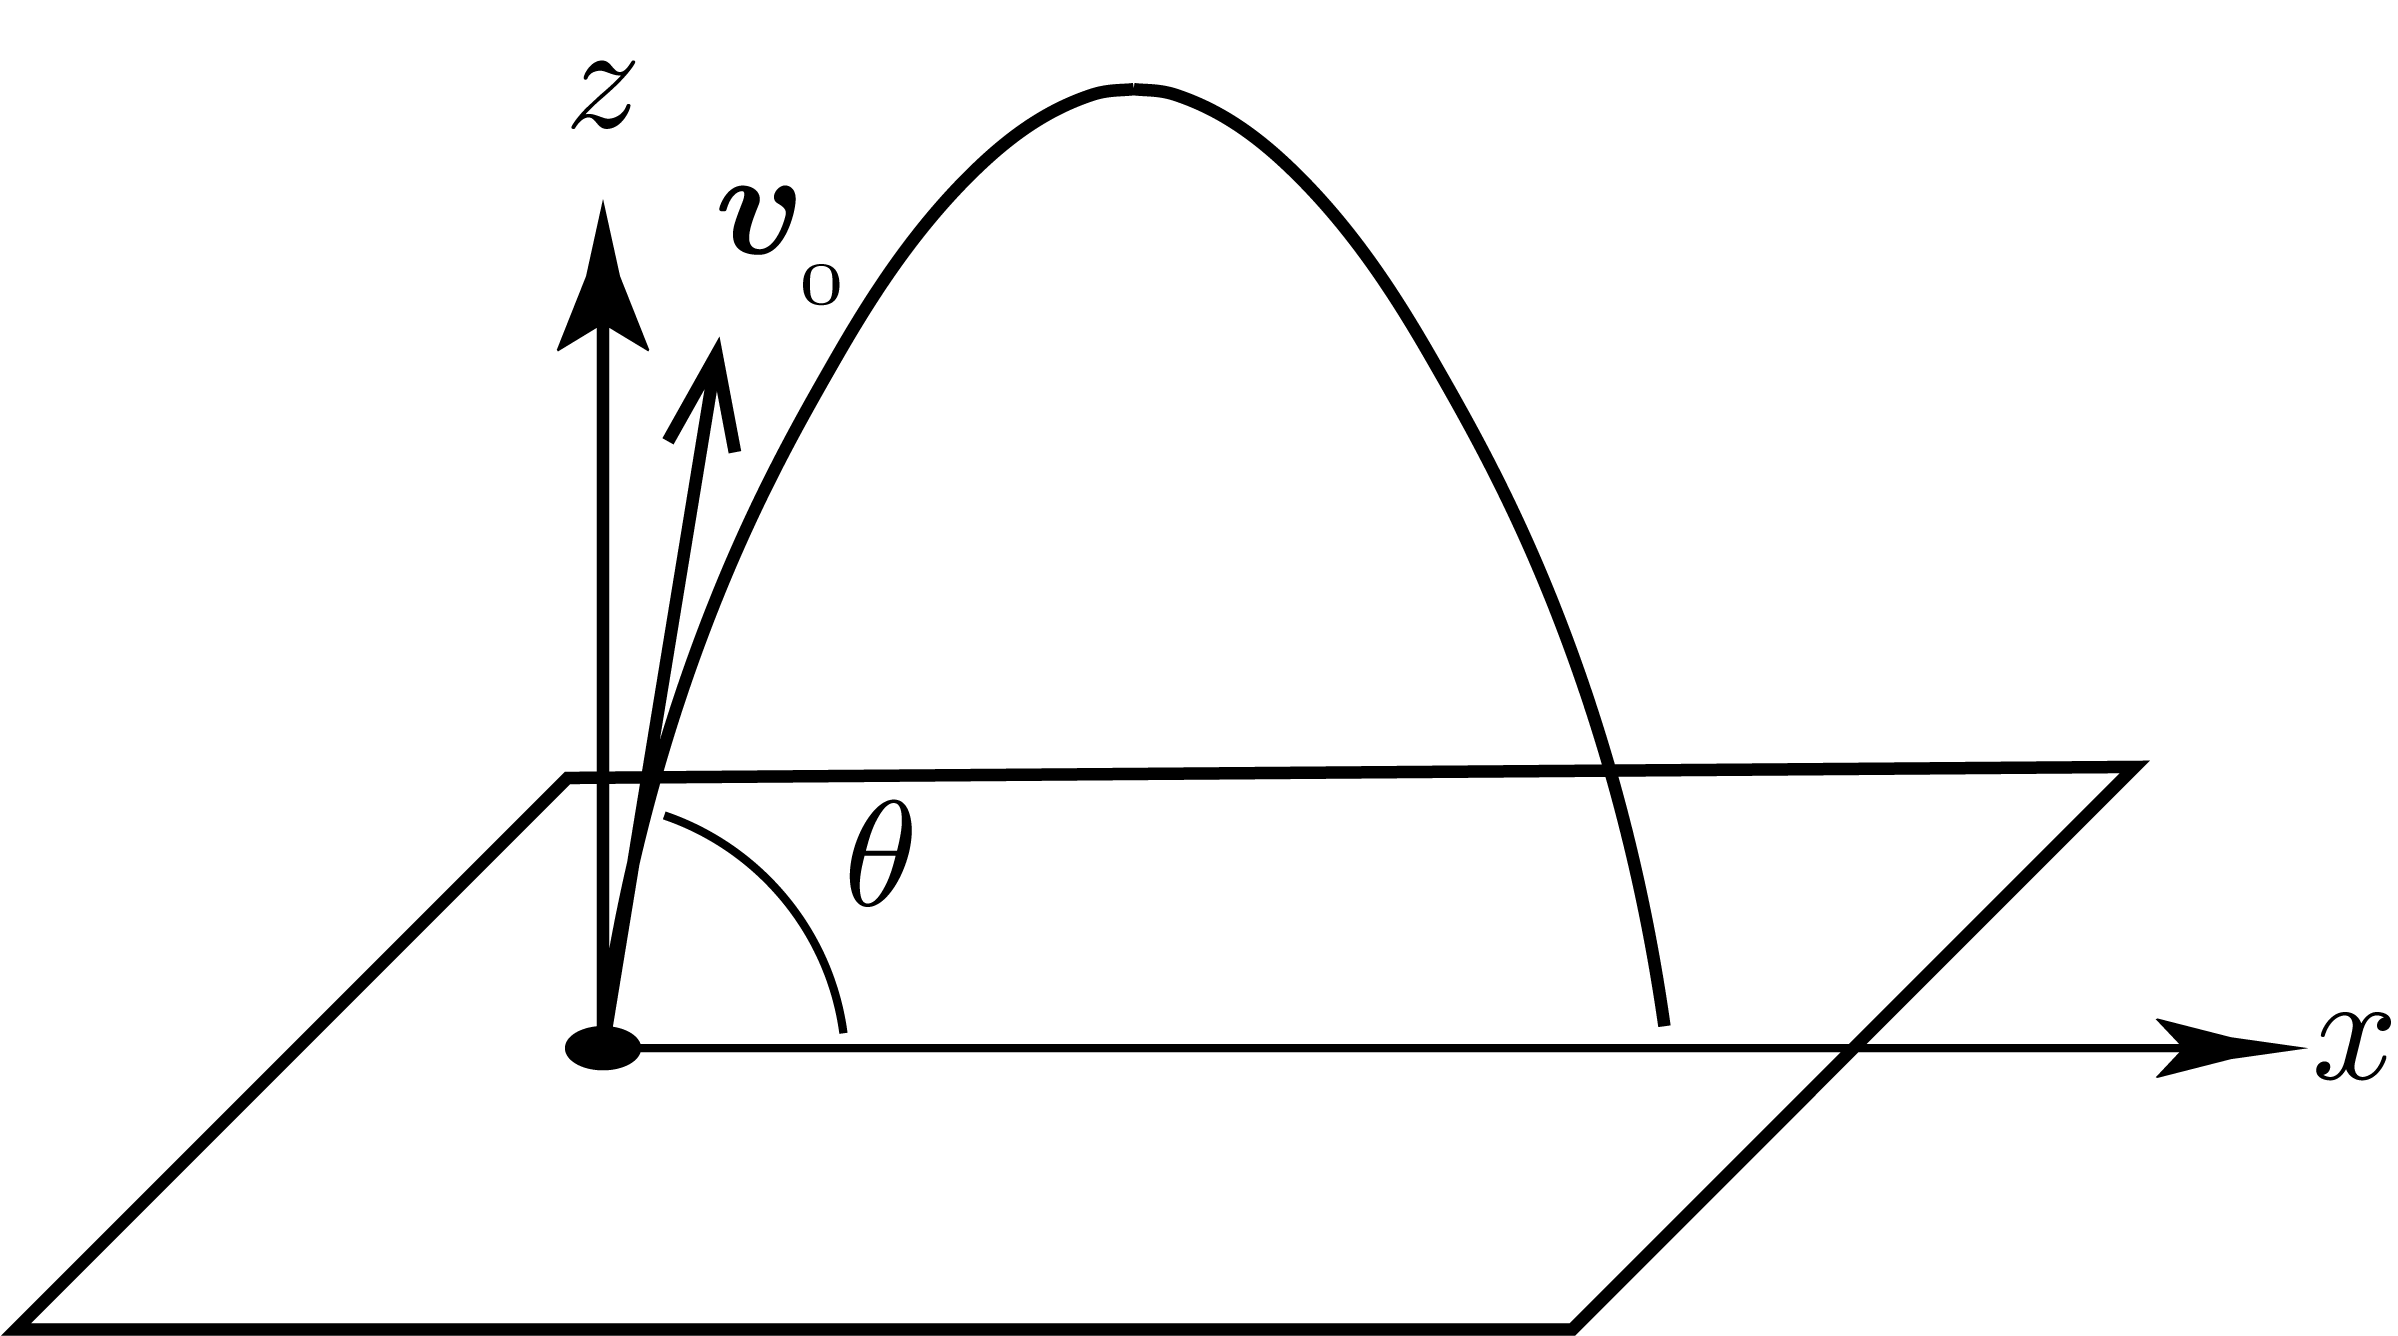
\includegraphics[width=7cm]{image/6-1-4.png}
\caption{抛体运动}
\end{wrapfigure}
在数学上看,\,这其实就是曲线方程:\,其参数方程的唯一给法.\,这样的式子就给出了几何学上的光滑曲线的定义.\,而不同于以往我们对曲线是$y=f(x)$的图像的刻板认识.\,但在这里,\,我们恰巧发现如果把参数$t$理解为时间的话,\,这恰好就对应到了一个粒子在三维空间中的运动,\,出于这样的原因,\,我们把反应了粒子位置随着时间变化的方程称为运动方程.\,它是\emph{轨迹方程}(function of trajactory)的一种特殊情况.\,对于轨迹方程,\,我们只需要通过符合方程的点$(x,\,y,\,z)$构成粒子所有运动中经过的位置构成的集合即可.\,例如,\,在地面$z=0$出发以仰角$\varphi$斜抛一个物体.\,那就以出发点为原点建立坐标系,\,竖直向上为$z$轴,\,抛的方向向前为$x$轴.\,那么运动方程为:
\[\left\{\begin{array}{l} x=v_0 t\cos\varphi\\ z=v_0 t\sin\varphi - \dfrac{1}{2}gt^2\end{array}\right.\]

但是轨迹方程不仅可以写成以上形式,\,还可以消去$t$得到:
\[z=x\tan\varphi -\frac{gx^2}{2v_0^2}(1+\tan^2\varphi)\]

\vspace{0.2cm}
{\bf 2.\,平面极坐标系下的分解}

如果质点做平面运动,\,那么我们问题得到了简化.\,此时往往有些情形下我们关心从原点的观察者出发看质点的运动时,\,质点离观察者的距离和质点相对观察者的方位.\,故引入\emph{极坐标系}(polar coordinate system)是自然而然的做法.\,其步骤为:\,确定观察者位置为\emph{极点}(pole),\,引出一条原点出发的射线为\emph{极轴}(polar axis);\,测量质点位置到极点距离$r$为\emph{矢径}(radius);\,从极点指向质点位置形成矢量矢径$\bs{r}$,\,测量极轴绕极点沿指定的正方向旋转到与矢径重合时旋转的角度$\theta$为\emph{极角}(polar angle).\,描述质点的位置时,\,$(r,\,\theta)$即构成极坐标.

仍然,\,极坐标可以用来表示质点的唯一位置:\,只需要给出$(r,\,\theta)$就可以确定位置.\,所以只要知道函数$r(t),\,\theta(t)$就能够确定其运动,\,这便是极坐标下的运动方程.\,同理如果消去$t$就能得到另一类轨迹方程.\,只要物体运动轨迹不经过极点,\,我们总是取$r(t),\,\theta(t)$为光滑的函数.\,$\theta$的取值为$(-\infty,\,+\infty)$以保证运动的连续性.\,不过$\theta$相差$2k\pi,\,k\in\mathbb{Z}$的所有坐标表示运动过程中的同一位置.

例如,\,在之前的抛体运动中,\,如果取$z$轴为极轴,\,那么其极坐标下的运动方程为:
\[\left\{\begin{array}{l} r^2=(\bs{v}_0 t+\dfrac{1}{2}\bs{g}t^2)^2=\dfrac{1}{4}g^2t^4  -gv_0t^3\sin\varphi + v_0^2t^2\\[3pt] \tan\theta=\dfrac{2v_0 \cos\varphi}{2v_0 \sin\varphi-gt}\end{array}\right.\]

这会有利于我们分析一些问题.\,例如如果关心以何种倾角抛出一个物体,\,物体离我们的距离会越来越远?\,就只需要让$r$为关于$t$的增函数,\,除了对$r$求导的做法,\,一种更加明智的做法可能是注意到关系式:
\[\frac{\ud r}{\ud t}>0  \quad\Leftrightarrow\quad	\frac{\ud}{\ud t}(\frac{1}{2}r^2)>0\]
\begin{align*} 
\Leftrightarrow \frac{\ud}{\ud t}(\frac{1}{2}r^2)	&=\frac{\ud}{\ud t}(\frac{1}{2}{\bs{r}\cdot\bs{r}})=\bs{r}\cdot\bs{v}\\
																			&=(\bs{v}_0 t+\dfrac{1}{2}\bs{g}t^2)\cdot(\bs{v}_0 +\bs{g}t)>0\\
\end{align*}

\[\Leftrightarrow (\bs{v}_0 +\dfrac{1}{2}\bs{g}t)\cdot(\bs{v}_0 +\bs{g}t)=\dfrac{1}{2}g^2t^2  -\dfrac{3}{2}gv_0t\sin\varphi + v_0^2>0\]

这就化为求关于$t$的二次函数恒大于零的系数条件问题,\,结论是初等的:\,判别式小于零:
\[\left(\dfrac{3}{2}gv_0\sin\varphi\right)^2-4\left(\dfrac{1}{2}g^2 \right)(v_0^2)<0\quad \Rightarrow\quad \sin\varphi<\frac{2\sqrt{2}}{3}\]

\begin{wrapfigure}[12]{o}[-10pt]{6cm}\label{6-1-5}
\vspace{-0.4cm}
\centering
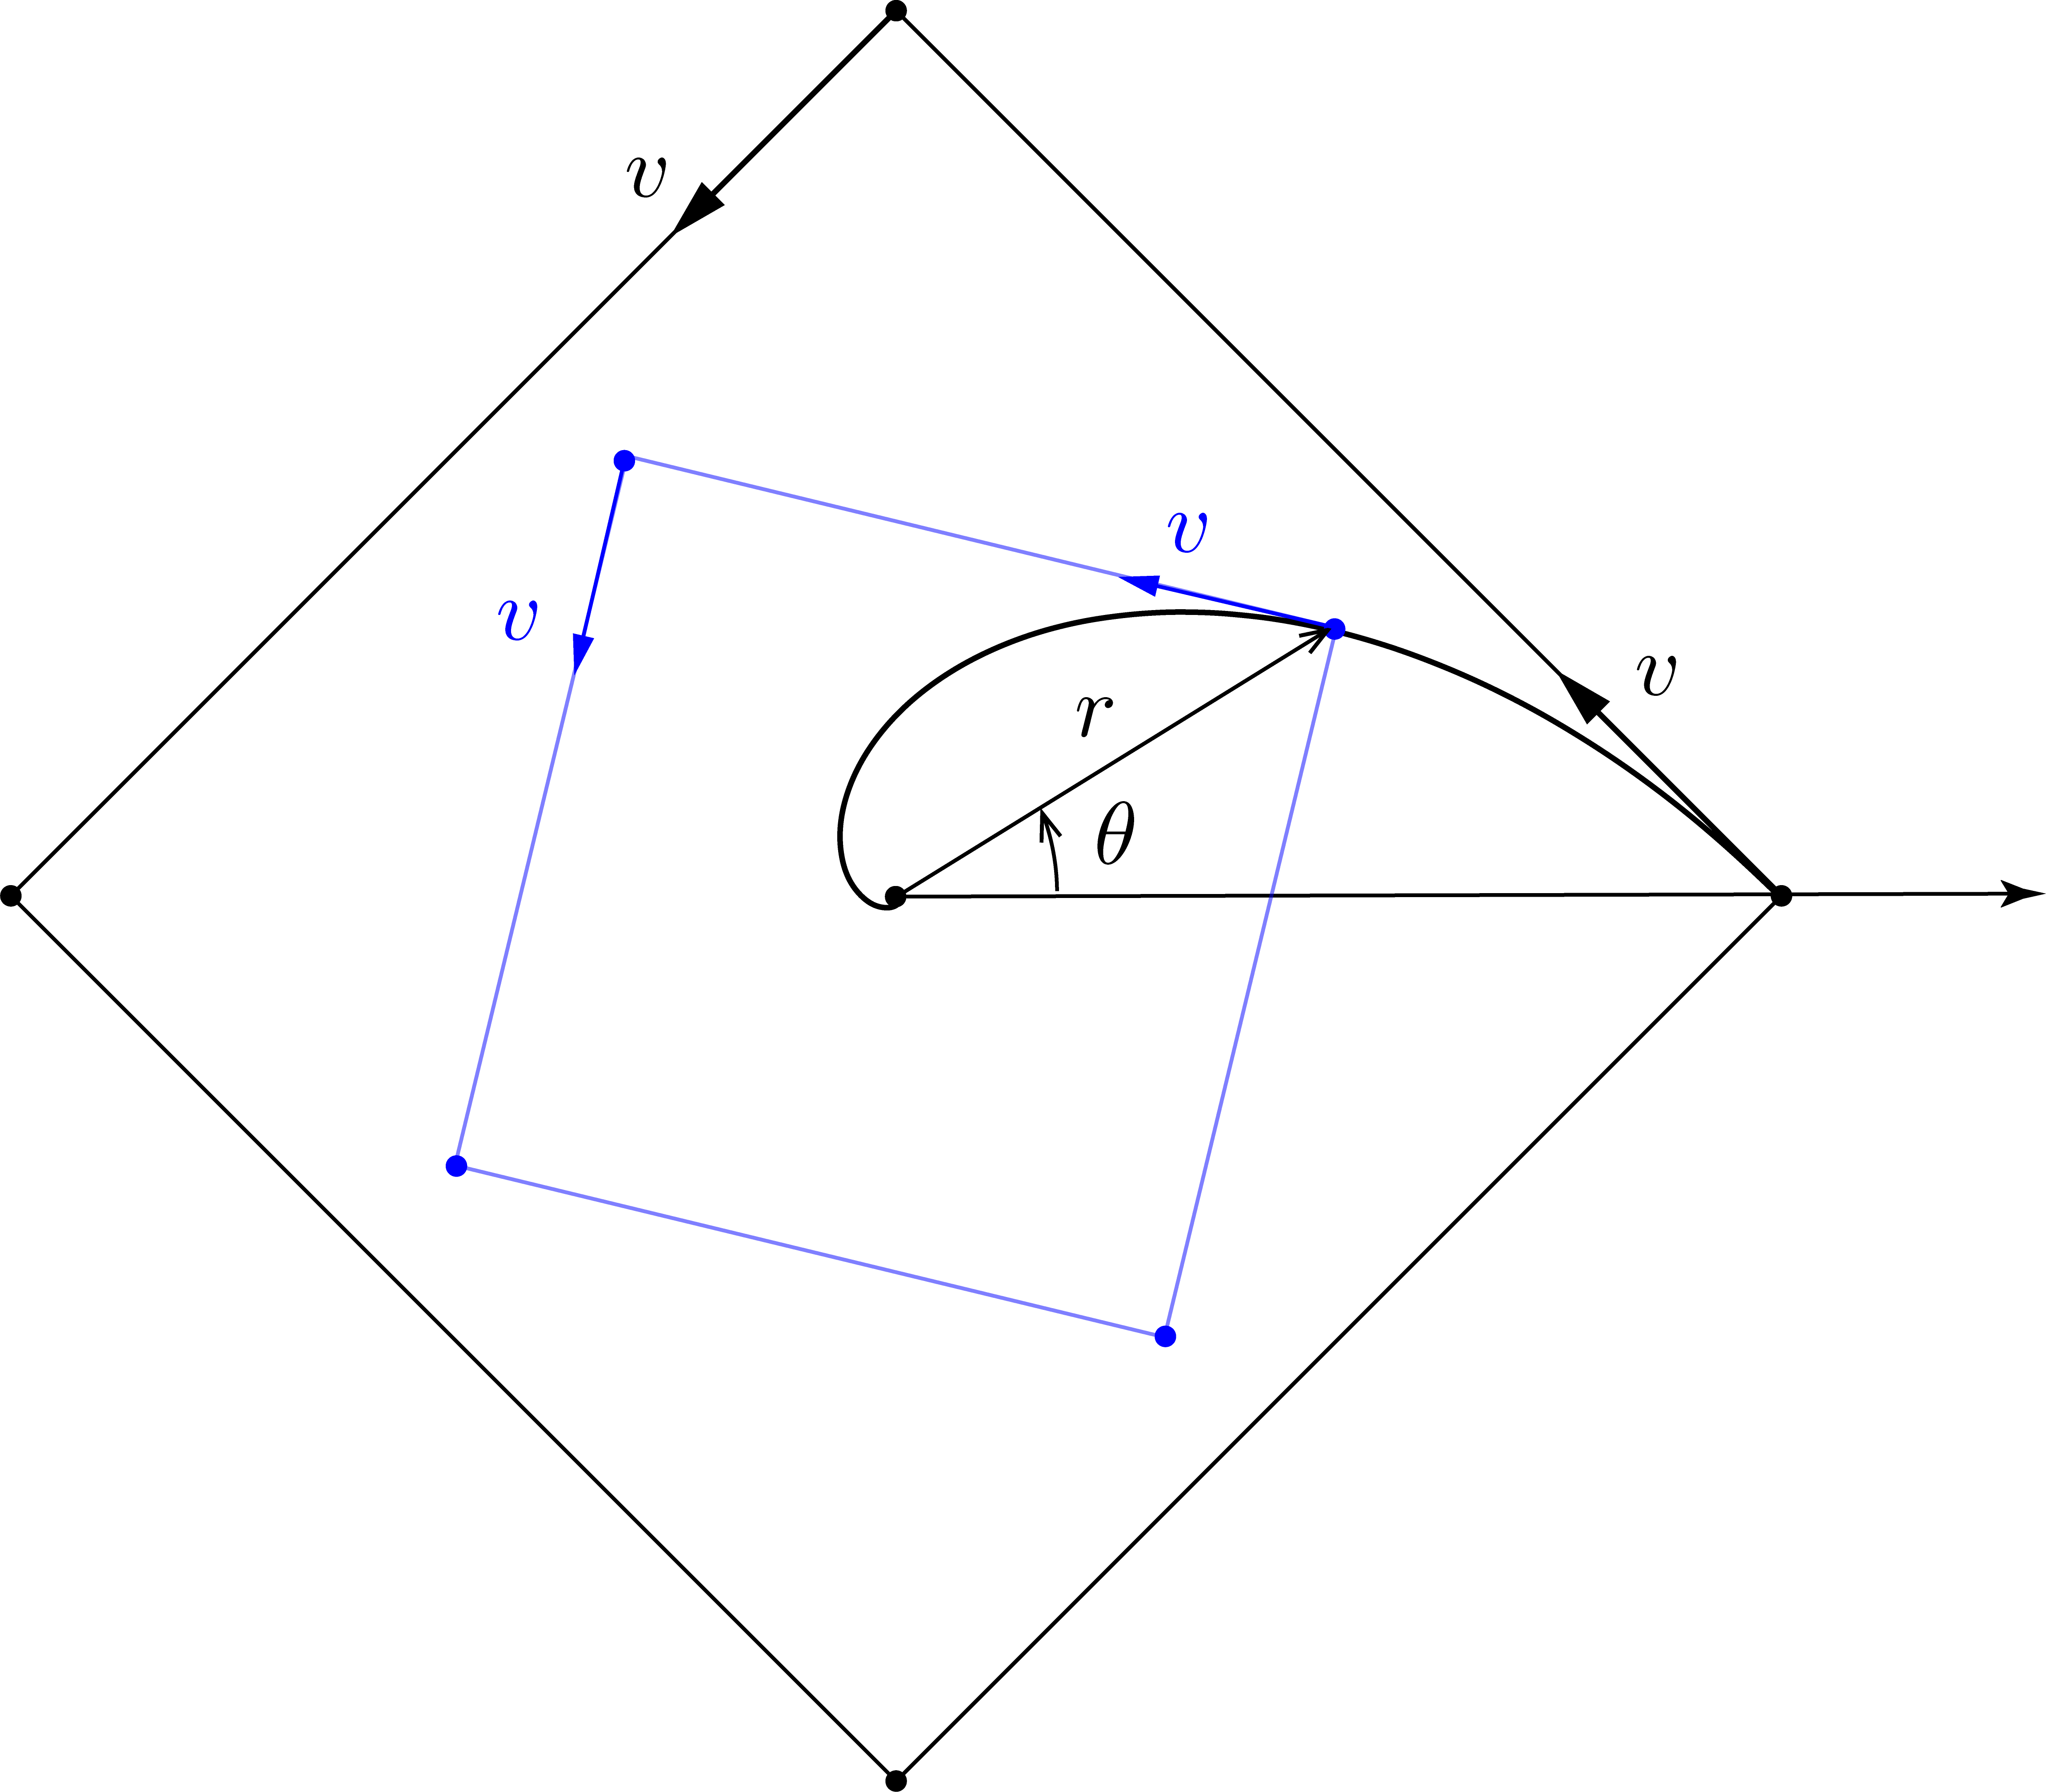
\includegraphics[width=6cm]{image/6-1-5.png}
\caption{首尾相追}
\end{wrapfigure}
采用极坐标系描述抛体运动也许是费力而不讨好的.\,但是描述其他一些运动又比直角坐标系存在天然的优势.\,比如一类经典追击问题的表述如下:\,四个平面运动的质点初始组成正方形.\,这个环形的结构中每一个质点都向着前一个质点运动发生追击.\,其中运动速度矢量具有变化的方向,\,即向着前方质点.\,但具有不变的速率$v$.\,确定物体的运动方程和轨迹.

对于这个问题,\,预先的关于物体在时间为$t$时的位置信息是几乎完全空缺的,\,但对于速度矢量我们知道一个信息:\,其大小为$v$.\,如果考虑直角坐标系,\,这个条件表示为:
\[|\bs{v}|=\sqrt{\dot{x}^2+\dot{y}^2}=v\]

但是对于位置和速度,\,我们还知道一个信息,\,就是它们夹钝角而且为$3\pi/4$.\,用直角坐标系的公式仔细化简的话也可以得到:
\[\tan \phi_{\bs{r}\curvearrowright \bs{v}}=-1\quad \Rightarrow \quad \frac{\bs{r}\cdot\bs{v}}{|\bs{r}\times \bs{v}|}=\frac{x\dot{x}+y\dot{y}}{x\dot{y}-y\dot{x}}=-1\]

\begin{wrapfigure}[12]{o}[-10pt]{6cm}\label{6-1-6}
\vspace{-0.4cm}
\centering
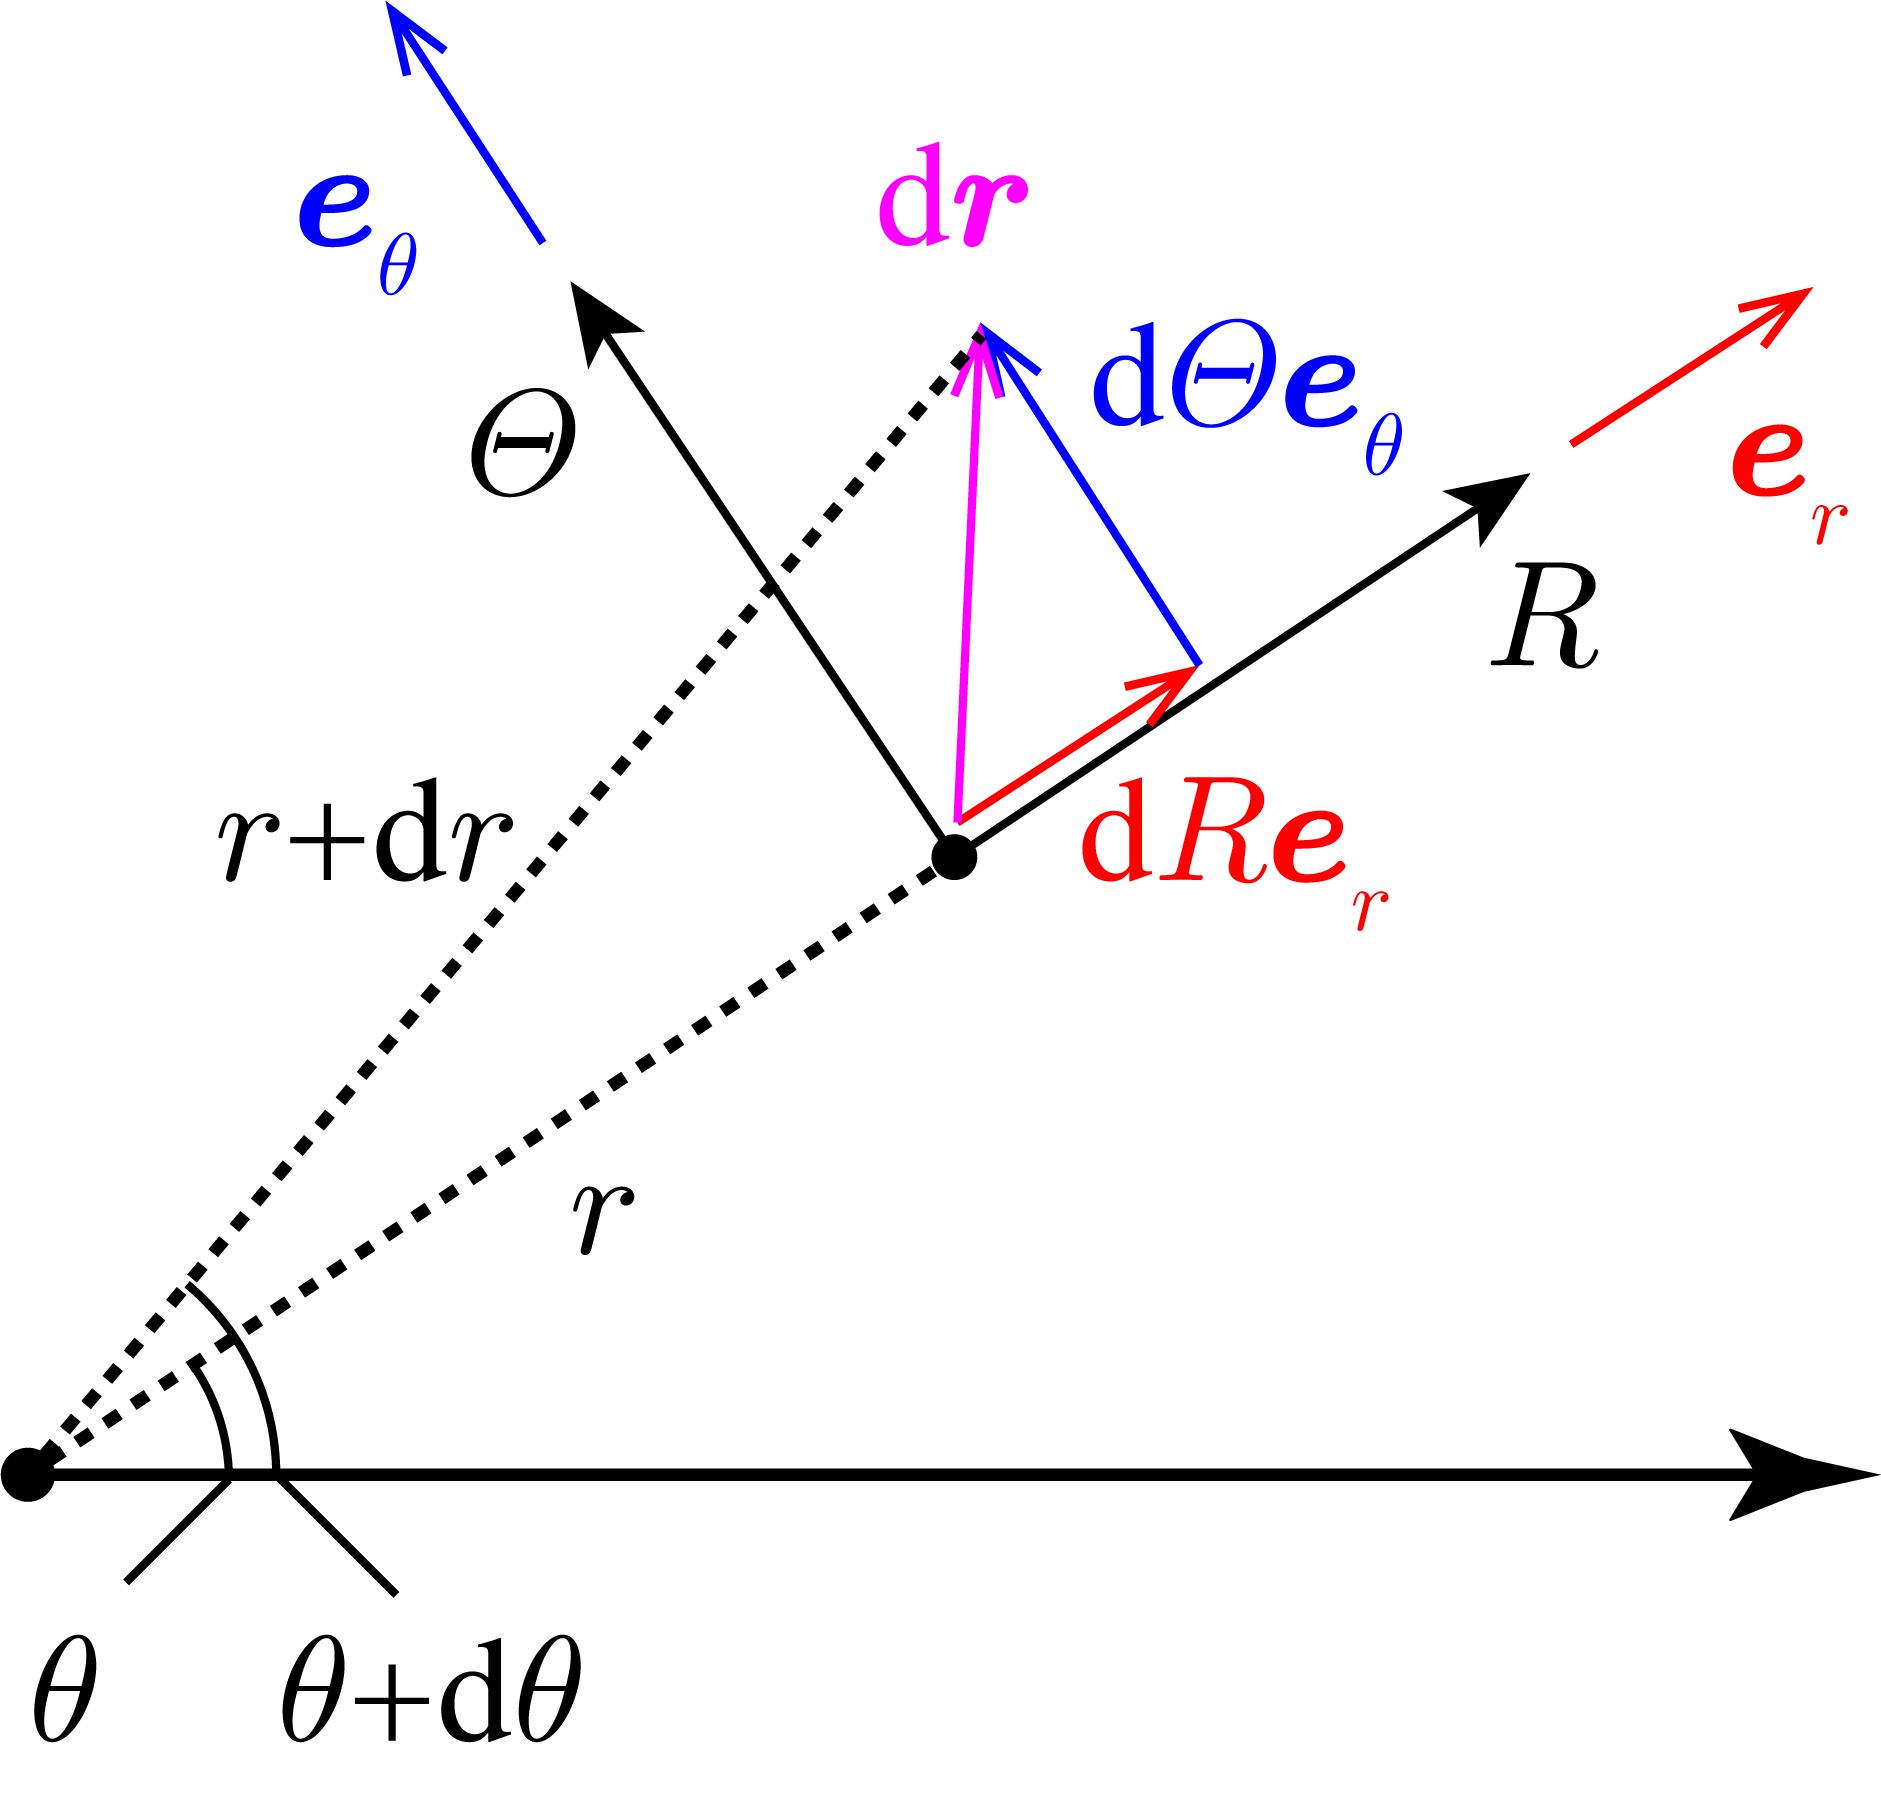
\includegraphics[width=6cm]{image/6-1-6.png}
\caption{极坐标系的活动框架}
\end{wrapfigure}
但这就较难求解\footnote{有兴趣的读者可以挑战一下.}.\,那么如果采用极坐标系会为我们带来何种新的思路呢?

那就是\emph{活动标架}(moving frame)的引入.\,无论粒子在何处,\,粒子的$\bs{r}$一定是作为了$r$和$\theta$的函数的.\,那么可以在粒子所在的点沿两个方向建立局域的$R-\varTheta$直角坐标系.\,这两个方向怎么确定呢?\,其实就是基矢的方向:
\[\bs{e}_r:=\frac{\partial\bs{r}}{\partial r}\left/\middle|\frac{\partial\bs{r}}{\partial r}\right|=\frac{\partial\bs{r}}{\partial r}\quad,\quad \bs{e}_\theta:=\frac{\partial\bs{r}}{\partial \theta}\left/\middle|\frac{\partial\bs{r}}{\partial \theta}\right|=\frac{1}{r}\frac{\partial\bs{r}}{\partial \theta}\]

上式中后一个偏导数的模为$r$是显然的.\,只需要考虑到圆的弧长和半径的关系即可.

局域的标架给我们什么方便?\,我们由偏导数和全微分的法则可以描述局域物体的微小位移.\,本质上,\,这相当于$\ud r$和$\ud \theta$导致的位矢$\bs{r}$改变$\ud \bs{r}$:
\[\ud \bs{r}_{(\ud r,\,\ud \theta)}=\ud \bs{r}_{(\ud r,\,0)}+\ud \bs{r}_{(0,\,\ud \theta)}=\ud R\bs{e}_r+\ud \varTheta\bs{e}_\theta\]
\[\ud \bs{r}_{(\ud r,\,\ud \theta)}=\frac{\partial \bs{r}}{\partial r}\ud r+\frac{\partial \bs{r}}{\partial \theta}\ud \theta=\ud r\bs{e}_r+r\ud \theta \bs{e}_\theta\]
\[\Rightarrow \quad \ud R=\ud r\;,\;\ud \varTheta=r\ud \theta\]

可见在曲线坐标情形下坐标的改变量$\ud r,\,\ud \theta$与在对应质点位移方向走过的弧长$\ud R,\,\ud \varTheta$的值一般是不一样的.\,它们之前的比值(弧长/坐标变化)称作\emph{拉梅系数}(Lam\'e coefficient).

\vspace{0.5cm}
既然叫做活动标架法,\,那么显然随着粒子的运动,\,两个基矢$\bs{e}_r,\,\bs{e}_\theta$的方向也在不断改变中.\,我们用极坐标,\,就是把一个物理量$\bs{A}$分解到粒子运动的瞬时局域坐标系中:
\[\bs{A}=A_r\bs{e}_r+A_\theta\bs{e}_\theta\]

那么在粒子发生运动后,\,以上矢量的改变应当由四部分组合而成:
\[\ud \bs{A}=\ud'\bs{A}+\tilde{\ud}\bs{A} \]
\[\ud' \bs{A}:=\ud A_r\bs{e}_r+\ud A_\theta\bs{e}_\theta\]
\[\tilde{\ud}\bs{A}:= A_r\ud\bs{e}_r+ A_\theta\ud\bs{e}_\theta\]

其中$\ud'$表示相对变化,\,类似于选取跟随旋转的活动标架而旋转的参考系后,\,矢量的变化量,\,故基矢自己的变化是被无视了的.\,而原来的$\ud$才表示绝对的变化.\,而$\tilde{\ud}$所带来的变化称作牵连变化或随体变化.\,它是即使前面的相对变化为零也会带来的,\,由于标架的``拉拽''导致的旋转带来的改变.\,事实上很容易证明其中的:
\[\ud \bs{e}_r=\ud \bs{\theta}\times \bs{e}_r=+\ud \theta \bs{e}_\theta\]
\[\ud \bs{e}_\theta=\ud \bs{\theta}\times \bs{e}_\theta=-\ud \theta \bs{e}_r\]

其中$\ud \bs{\theta}$是方向垂直于纸面向外的,\,大小即极坐标下物体坐标之角坐标的增量$\ud \theta$.

这就足以给出:
\[(\ud \bs{A})_r=\ud A_r-A_\theta \ud \theta\]
\[(\ud \bs{A})_\theta=\ud A_\theta+A_r \ud \theta\]
\newpage
两边再同时除以时间,\,我们得到粒子运动过程中一个矢量导数的两个分量与这矢量两个分量的导数之间的关系:
\[(\dot{\bs{A}})_r=\dot{A_r}-\dot{\theta}A_\theta\]
\[(\dot{\bs{A}})_\theta=\dot{A_\theta}+\dot{\theta}A_r\]

导数的分量不等于分量的导数,\,这也是坐标系的弯曲所带来的.\,数学上,\,这意味算符$\partial_t$与算符$\bs{e}\cdot$的\emph{不对易性}(non-commutative):
\[\bs{e}\cdot(\partial_t \bs{A})\neq \partial_t(\bs{e}\cdot \bs{A})\]

通过这个原理,\,我们可以推理得到:
\[\bs{r}=r\bs{e}_r+0\bs{e}_\theta\quad \Rightarrow\quad r_r=r\,,\,r_\theta=0\]
\[\bs{v}=\dot{\bs{r}}\quad \Rightarrow\quad  v_r=\dot{r_r}-\dot{\theta}r_\theta=\dot{r}\,,\,v_\theta=\dot{r_\theta}+\dot{\theta}r_r=\dot{\theta}r\]
\[\bs{a}=\dot{\bs{v}}\quad \Rightarrow\quad  a_r=\dot{v_r}-\dot{\theta}v_\theta=\ddot{r}-\dot{\theta}^2r\,,\,a_\theta=\dot{v_\theta}+\dot{\theta}v_r=\ddot{\theta}r+2\dot{\theta}\dot{r}\]

这个操作甚至可以继续下去,\,计算急动度等:
\[\bs{j}=\dot{\bs{a}}\quad \Rightarrow \quad j_r=\dot{a_r}-\dot{\theta}a_\theta=\dddot{r}-3\dot{\theta}\ddot{\theta}r-3\dot{\theta}^2\dot{r}\,,\,j_\theta=\dot{a_\theta}+\dot{\theta}a_r=\dddot{\theta}r+3\ddot{\theta}\dot{r}+3\dot{\theta}\ddot{r}-\dot{\theta}^3r\]
\[\cdots\]

极坐标下速度,\,加速度的公式是非常常用的,\,它们是:
\[\bs{v}=(\dot{r}\,,\,\dot{\theta}r)\quad\bs{a}=(\ddot{r}-\dot{\theta}^2r\,,\,\ddot{\theta}r+2\dot{\theta}\dot{r})\]

故,\,在之前的首尾相追问题\ref{6-1-5}中以正方形中心为原点,\,以初始位置为极轴方向建立极坐标系.\,那么两个条件:\,速度大小恒定为$v$和位矢速度夹角恒定$3\pi/4$表述为:
\[v_r^2+v_\theta^2=v^2\quad ,\quad \frac{v_\theta}{v_r}=-1\]

相当容易解出来两个分速度的值,\,再结合之前的速度公式:
\[\dot{r}=-\frac{\sqrt{2}}{2}v\quad ,\quad \dot{\theta}r=\frac{\sqrt{2}}{2}v\]

这样,\,便可以轻松解出运动方程来,\,结合初始条件,\,不妨设初始矢径为$r_0$,\,幅角为$0$:
\[\dot{r}=-\frac{v}{\sqrt{2}}\quad \Rightarrow \quad r=r_0-\frac{vt}{\sqrt{2}}\]
\[\dot{\theta}=\frac{v}{\sqrt{2}r_0-vt}\quad \Rightarrow \quad  \theta =-\ln\left(1-\frac{vt}{\sqrt{2}r_0}\right)\]

轨迹方程通过上述方程消参即可.\,但也可以通过之前的微分方程相除得到新微分方程求解,\,曲线为\emph{对数螺线}(logarithmic spiral):
\[\frac{\ud r}{\ud \theta}=-r\quad \Rightarrow \quad r=r_0\ue^{-\theta}\]

平面的极坐标系在三维空间的推广为\emph{柱坐标系}(cylindrical coordinate system)和\emph{球坐标系}(spherical coordinate system).\,类似公式的核心也与平面极坐标相差无几,\,都在于活动标架的基矢微分.\,请读者自行推导.

\vspace{0.2cm}
{\bf 3.\,自然坐标系下的分解}

设想仍然采用活动标架法的思路,\,但是,\,标架的方向不再由粒子的位置相对事先建立的背景的坐标系的关系而决定.\,而是紧密地由粒子运动的性质:\,瞬时的速度方向,\,轨迹曲线的弯曲方向等决定.\,那么我们就得到了特殊的标架:\,\emph{自然坐标系}(natural coordinates).

自然坐标系的建立是派生于粒子运动的轨迹的那条曲线的性质的.\,借助牛顿等人创立的微积分与笛卡尔等人创立的解析几何的帮助,\,对于光滑曲线曲面的性质的研究构成了\emph{古典微分几何}(classical differential geometry)的主要课题.\,

我们考虑三维空间问题.\,对于一条空间曲线.\,它总是一些点的集合,\,而如果规定某个起始点以后,\,每一个点都会有一个$s$坐标,\,它就是从起始点到这个点的弧长.\,而其实我们可以把$s$视作一个自变量,\,因为$s$改变而改变的是不同点的位置$\bs{r}$.\,也就是说$\bs{r}(s)$作为了$s$的函数.\,那么这个曲线在某一点处的切矢量就可以被自然地定义为:
\[\bs{\tau}=\frac{\ud \bs{r}}{\ud s}\]

\begin{wrapfigure}[14]{o}[-10pt]{6cm}\label{6-1-7}
\vspace{-0.2cm}
\centering
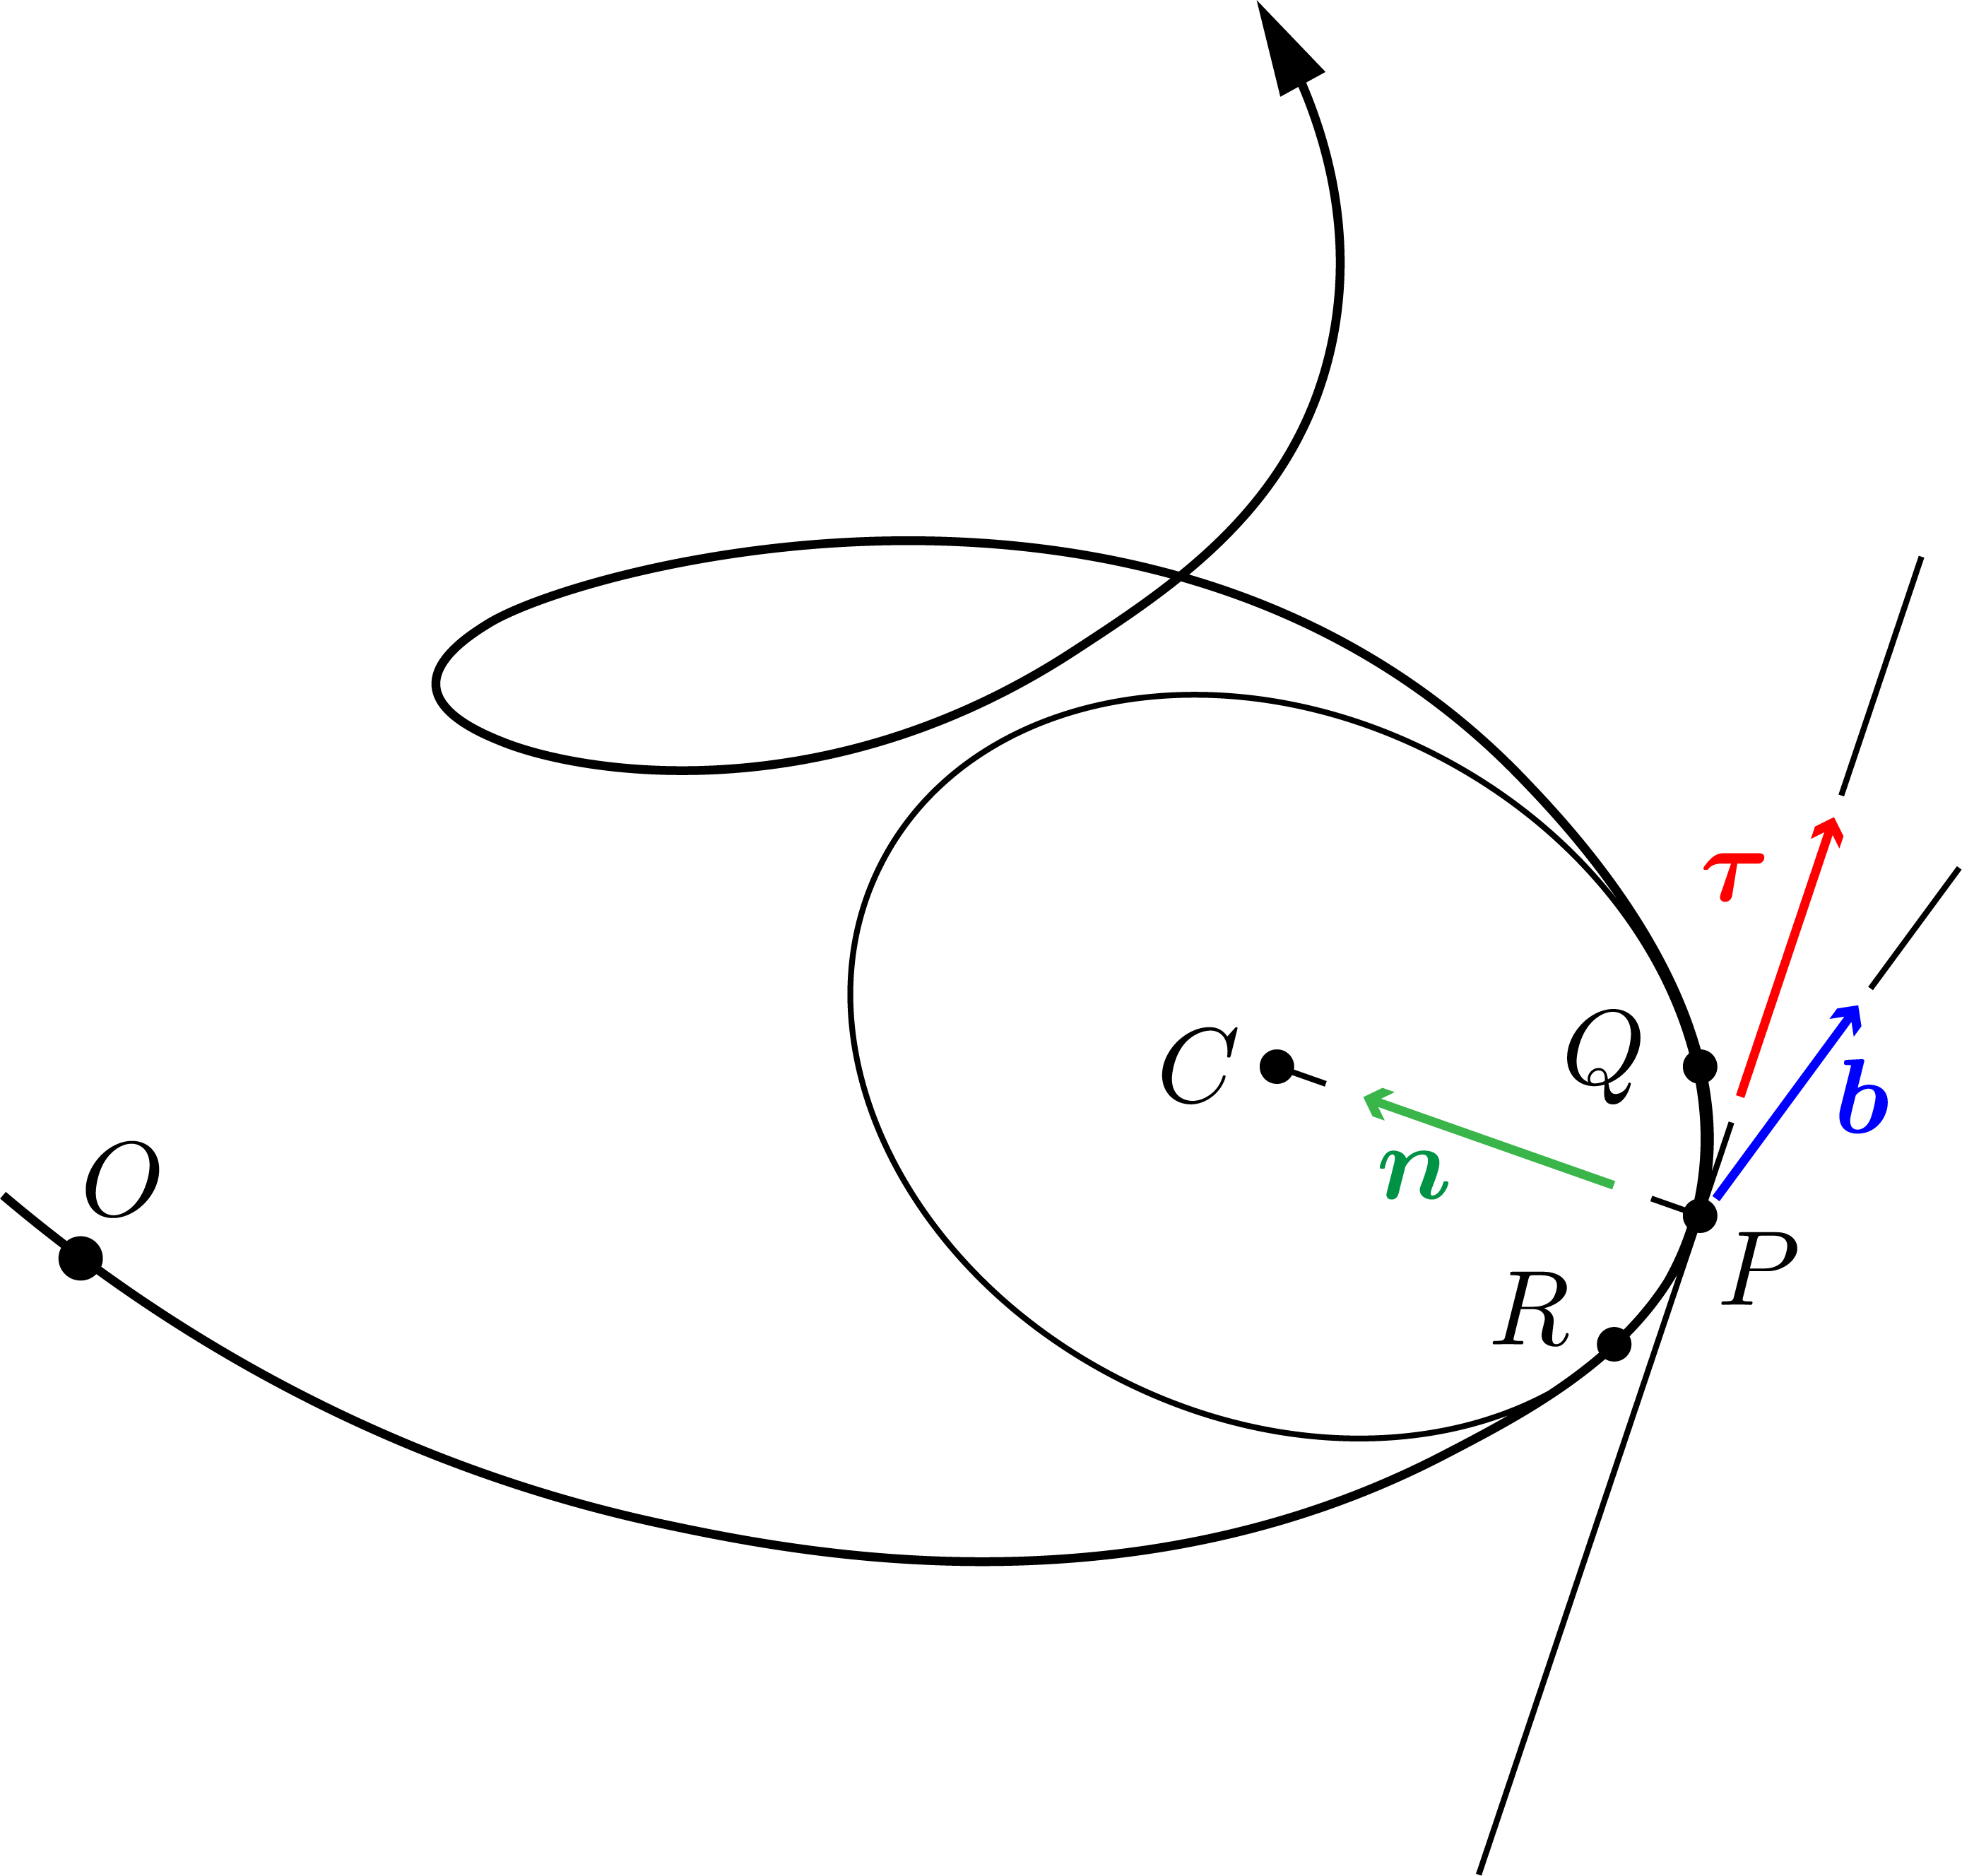
\includegraphics[width=6cm]{image/6-1-7.png}
\caption{Frenet框架}
\end{wrapfigure}
以上矢量模自然为$1$.\,因为分子$\ud \bs{r}$的长度就是分母的$\ud s$.\,方向则是在曲线的\emph{切线}(tangent line)方向.\,切线是这样一种线:\,曲线上有一点$P$.\,如果在$P$两侧任取一个点$Q$并连接$PQ$,\,使$Q$无限接近$P$即$\ud s \to 0$,\,那么$PQ$所在的直线的极限就是$P$点的切线.\,这又引申出第二个概念:\,如果在$P$所有各取一个点$Q,\,R$.\,那么$PQR$三点确定的圆也将随着$Q,\,R$同时无限接近于$P$而具有极限.\,这个圆叫做\emph{密切圆}或\emph{曲率圆}(osculating circle).\,其所在的平面叫做\emph{密切平面}(osculating plane).\,而圆心$C$为\emph{曲率中心}(center of curvature),\,最后,\,实际上$P$到$C$的方向就是\emph{法}(normal)方向,\,该方向的单位矢量叫做法矢量$\bs{n}$.\,而副法矢量$\bs{\tau}\times\bs{n}=\bs{\beta}$所决定的方向为\emph{副法}(binormal)方向.\,这样三个矢量便构成\emph{弗雷内框架}(Frenet frame)或称TNB框架.

事实上,\,如果计算曲线在过程中的转向,\,它可以用三个矢量方向的变化来表示.\,如果计算三个矢量对$\ud s$的变化率,\,一定能写作:
\[\begin{array}{rlll}
\frac{\ud \bs{\tau}}{\ud s}=		&	+0\bs{\tau} 	&	+k\bs{n} 		& +\varepsilon\bs{\beta}\\
\frac{\ud \bs{n}}{\ud s}=		&	-k\bs{\tau} 	&	+0\bs{n} 		& +\gamma\bs{\beta}\\
\frac{\ud \bs{\beta}}{\ud s}=		&	-\varepsilon\bs{\tau} 	&	-\gamma\bs{n} 		& +0\bs{\beta}
\end{array}\]

这是因为框架一定要具有正交归一的一套基矢量,\,而且这个性质在曲线上任何一点都要成立,\,指的是以下六个式子:
\[\bs{\tau}\cdot\bs{\tau}=1\quad,\quad\bs{n}\cdot\bs{n}=1\quad,\quad \bs{\beta}\cdot\bs{\beta}=1\]
\[\bs{\tau}\cdot\bs{n}=0\quad,\quad\bs{n}\cdot\bs{\beta}=0\quad,\quad \bs{\beta}\cdot\bs{\tau}=0\]

对六个式子分别求导数就看出来了,\,\emph{一个单位矢量自己的导数必然垂直于自身},\,从而三个基矢导数在自己上的投影都必须为零.\,而两个不同基矢的导数互相在对方方向的投影则会正负相消,\,这样才能保证两个矢量始终正交.\,就能理解之前的$9$个系数为什么要写成这个形式.

最后我们指出,\,系数$\varepsilon$应当是$0$.\,这是因为作为法线方向的定义本身,\,它就应当在$\bs{\tau}$的变化量$\ud\bs{\tau}$所在的方向上.\,从而第一个式子不会具有$\bs{\beta}$方向的分量.\,综上所述,\,我们得到了:

\[\begin{array}{rlll}
\frac{\ud \bs{\tau}}{\ud s}=		&	 	&	+k\bs{n} 		& \\
\frac{\ud \bs{n}}{\ud s}=		&	-k\bs{\tau} 	&	 		& +\gamma\bs{\beta}\\
\frac{\ud \bs{\beta}}{\ud s}=		&	 	&	-\gamma\bs{n} 		& 
\end{array}\]

这就是\emph{弗雷内公式}(Frenet formulae).\,其中$k$称作曲线的\emph{曲率}(curvature).\,它的意义是衡量了曲线方向转动的快慢,\,事实上由于曲线切线的无穷小转动角度其实在竖直上恰好会等于无穷小矢量$\ud\bs{\tau}$的长度,\,从而有:
\[k=\abs{\frac{\ud\bs{\tau}}{\ud s}}=\frac{\ud\theta}{\ud s}\]

即,\,曲率为:\,质点沿曲线走单位长度所转过的角度.\,曲率半径实际上是曲率的倒数.\,它是曲率圆的半径$\rho=1/k$.

而$\gamma$则被称作\emph{挠率}(torsion).\,我们通过弗雷内公式的第三式可以发现,\,挠率反映了副法矢量,\,或者说被复法矢量作为法平面的密切平面,\,绕曲线此时的切线的旋转快慢.\,它使得粒子瞬时运动的那个平面在改变着.\,下面我们会发现,\,实际上挠率对运动学中直到加速度的表达式都是没有任何贡献的.

如何用自然法描述粒子的运动?\,事实上这就相当于把粒子运动的路程$s$和三个矢量$\bs{\tau},\,\bs{n},\,\bs{\beta}$都表示为时间的函数:
\[s(t),\,\bs{\tau}(t),\,\bs{n}(t),\,\bs{\beta}(t)\]

但事实上,\,曲线本身轨迹必须先存在才能让我们事先确定好框架,\,而这样一个曲线其实本身由$\bs{r}(s)$给出,\,而且满足:
\[\frac{\ud \bs{r}}{\ud s}=\bs{\tau}\quad,\quad \frac{\ud^2 \bs{r}}{\ud s^2}=k\bs{n}\quad,\quad \frac{\ud^3 \bs{r}}{\ud s^3}=-k^2\bs{\tau}+\frac{\ud k}{\ud s}\bs{n}+k\gamma\bs{\beta}\]

然后我们唯一要做的就是给出$s(t)$函数,\,这一定可以帮助我们确定运动的各个量.

事实上,\,由于泰勒展开公式,\,近似到三阶:
\[\Delta \bs{r}\simeq\frac{\ud \bs{r}}{\ud s}\ud s+\frac{1}{2}\frac{\ud^2 \bs{r}}{\ud s^2}\ud s^2+\frac{1}{6}\frac{\ud^3 \bs{r}}{\ud s^3}\ud s^3=(k\ud s-\frac{k^2}{6}\ud s^3)\bs{\tau}+(\frac{k}{2}\ud s^2+\frac{1}{6}\frac{\ud k}{\ud s}\ud s^3)\bs{n}+\frac{k\gamma}{6}\ud s^3\bs{\beta}\]

如果只保留领头项,\,忽略高阶小量.\,我们就得到,\,在粒子运动的局域坐标系中,\,位移$\ud s$长度到达的点三个坐标$T,\,N,\,B$分别近似为:
\[T=\ud s \quad,\quad N=\frac{k}{2}\ud s^2 \quad,\quad B=\frac{k\gamma}{6}\ud s^3\]

仍然考虑之前的三阶近似下的严格$\Delta \bs{r}$与$\ud{s}$的关系,\,这一次代入$s(t)$的三阶套了展开:
\[\ud s\simeq \dot{s}\ud t+\frac{\ddot{s}}{2}\ud t^2+\frac{\dddot{s}}{6}\ud t^3\]

我们整理$\ud t$的各阶项,\,最终得到:
\[\Delta \bs{r}\simeq \bs{v}\ud t+\frac{1}{2}\bs{a}\ud t^2+\frac{1}{6}\bs{j}\ud t^3\]

其中速度与加速度的公式为:
\[\bs{v}=\dot{s}\bs{\tau}\]
\[\bs{a}=\ddot{s}\bs{\tau}+k\dot{s}^2\bs{n}\]

速度方向必然沿切向,\,大小上就等于$\dot{s}$,\,即单位时间走过的弧长.\,而加速度则有两个分量.\,一是由于速率在增减导致的切向加速度,\,大小等于$a_\tau=\ddot{s}$;\,第二项则是由于曲线的弯曲导致的法向加速度.\,它的值为$a_n=\dot{s}^2/\rho$.\,

如果要计算急动度等,\,可以从之前的泰勒展示中获得,\,其实还可以直接对加速度求导数,\,此时表达式会突然产生很多项:
\[\bs{j}=(\dddot{s}-k^2\dot{s}^3)\bs{\tau}+(3k\dot{s}\ddot{s}+\dot{k}\dot{s}^3)\bs{n}+k\gamma\dot{s}^3\bs{\beta}\]

利用自然坐标下的分解方式,\,如果已经直到特定曲线的曲率,\,就可以根据质点在曲线上的运动方式来计算运动的加速度.\,但是反过来利用运动学公式来确定曲线的曲率半径也不失为一种极其简单的做法.\,我们注意到,\,利用加速度在垂直于速度方向的那个分量即为$v^2/\rho$的结论,\,可以得到:
\[\rho=\frac{\bs{v}^3}{\abs{\bs{a}\times\bs{v}}}\]

例如,\,如果已知二维空间中的曲线方程$y=f(x)$.\,那么如果命一质点在曲线上运动且满足$x=t,\,y=f(t)$,\,那么速度为$\bs{v}=(1,\,f')$,\,加速度为$\bs{a}=(0,f'')$.\,利用上式可得:
\[\rho=\frac{(1+f'^2)^\frac{3}{2}}{\abs{f''}}\]

再例如.\,之前的首尾相追问题中,\,曲线对数螺线写作:
\[r=a\ue^{k\theta}\]

如何计算曲率半径?\,我们让粒子在曲线上绕极点做匀速旋转,\,也就是:
\[\theta=\omega t\quad,\quad r=a\ue^{k\omega t}\]

那么借助极坐标的加速度公式得:
\[\bs{v}=(\dot{r},\,\dot{\theta}r)=(k\omega a\ue^{k\omega t},\,\omega a\ue^{k\omega t})=(k\omega r,\,\omega r)\]
\[\bs{a}=(\ddot{r}-\dot{\theta}^2r,\,\ddot{\theta}r+2\dot{\theta}\dot{r})=((k^2-1)\omega^2 a\ue^{k\omega t},\,2k\omega^2 a\ue^{k\omega t})=((k^2-1)\omega^2 r,\,2k\omega^2 r)\]

代入之前的曲率公式便可以得到:
\[\rho=\sqrt{1+k^2}r\]

\subsection{刚体的运动}

关于刚体的运动,\,它的定义我们其实将在之后的刚体专门的章节又一次做更进一步的探讨.\,初步我们认为所谓刚体就是这样一种物体:\,存在一个特殊的参考系(平动或转动)能够使得该物体上每一个点都每时每刻相对静止.\,但是这样我们又涉及到下一节才讲的参考系的概念.\,在此我们又不得不早于预期提及.

\begin{wrapfigure}[12]{o}[-10pt]{6cm}\label{6-1-8}
\vspace{-0.2cm}
\centering
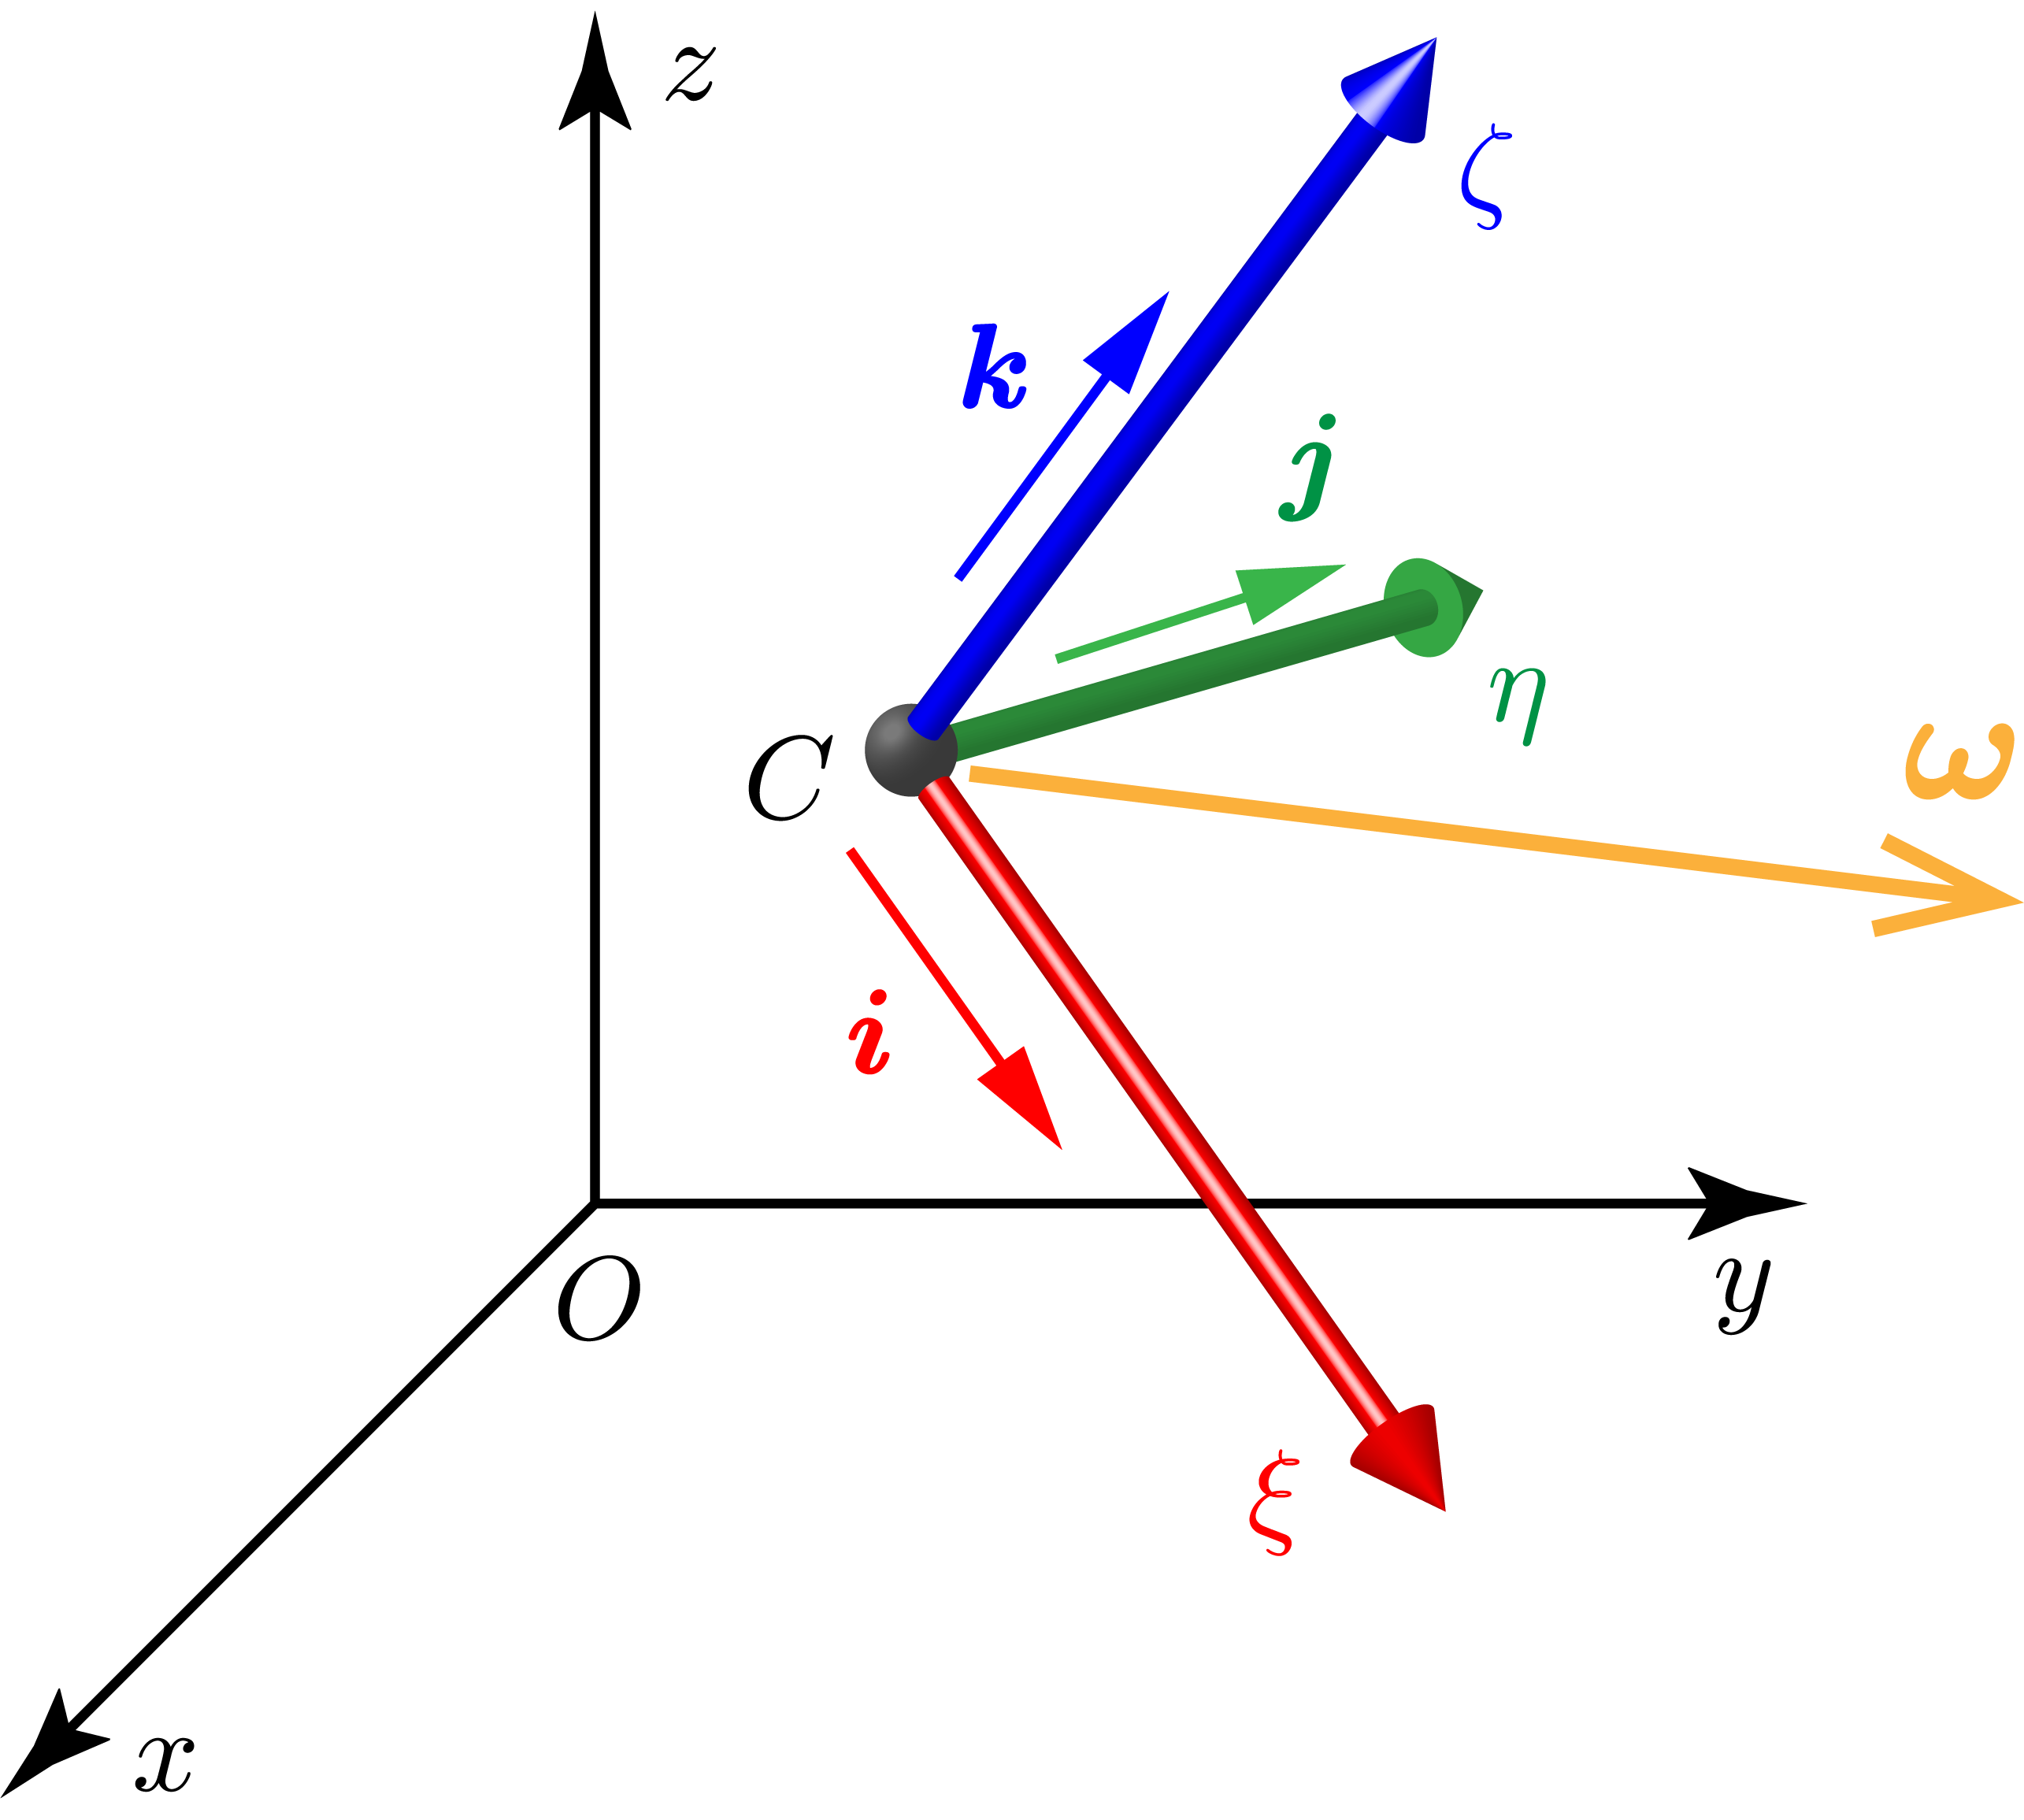
\includegraphics[width=6cm]{image/6-1-8.png}
\caption{刚体的本征框架}
\end{wrapfigure}
为此我们换一种更加直观的方式引入这些概念而不是去严格定义刚体与参考系的概念.\,设想我们有一个正交的刚性框架,\,即三条射线状坐标轴构成的物体,\,下称$\xi,\,\eta,\,\zeta$轴,\,该框架就会自然造成四个矢量.\,首先是框架原点$C$的位置矢量$\bs{r}$.\,其次是三坐标轴方向的三个基矢\footnote{原来的基矢方向记做$\bs{e}_{x,\,y,\,z}$.}$\bs{i},\,\bs{j},\,\bs{k}$.\,它们都会随着时间变化,\,可以用四个导数表征.\,其中$\bs{v}=\dot{\bs{r}},\,\bs{a}=\ddot{\bs{r}}$.\,但是,\,对于三个基矢导数有没有更加简单的描述方法呢?\,如果我们把三个基矢导数就向三个基矢本来的方向分解\footnote{由于字母$i,\,j$上本来就有点,\,所以在符号上约定遇到要在这两个字母上加点时改为横向$\ddot{\imath},\,\ddot{\jmath}$.\,偶尔也见到反而去掉点的$\imath,\,\jmath$.\,出于这样无法表示高阶导数,\,我们不采用这种模式.}:
\[\begin{array}{rlll}
\bs{\ddot{\imath}}=		&	+\omega_{11}\bs{i} 	&	+\omega_{12}\bs{j} 		& +\omega_{13}\bs{k}\\
\bs{\ddot{\jmath}}=		&	+\omega_{21}\bs{i} 	&	+\omega_{22}\bs{j} 		& +\omega_{23}\bs{k}\\
\bs{\dot{k}}=				&	+\omega_{31}\bs{i} 	&	+\omega_{32}\bs{j} 		& +\omega_{33}\bs{k}
\end{array}\]

依然,\,我们注意到出于以下正交归一的结构不会改变,\,在求导下为零,\,所以上述表达式中的九个系数反对称:
\[\frac{\ud}{\ud t}\left\{\begin{array}{cccc}
1= 	&\bs{i}\cdot\bs{i} 	&\bs{j}\cdot\bs{j} 	&\bs{k}\cdot\bs{k} 	\\
0= 	&\bs{i}\cdot\bs{j} 	&\bs{j}\cdot\bs{k} 	&\bs{k}\cdot\bs{i}
\end{array}\right\}=0\quad \Rightarrow \quad\omega_{ij}+\omega_{ji}=0\]

出于某种符号约定与对称的原因,\,我们把导数重新写作:
\[\begin{array}{rlll}
\bs{\ddot{\imath}}=		&									 	&	+\omega_3\bs{j} 				& -\omega_2\bs{k}\\
\bs{\ddot{\jmath}}=		&	-\omega_3\bs{i} 			&									 		& +\omega_1\bs{k}\\
\bs{\dot{k}}=				&	+\omega_2\bs{i} 			&	-\omega_1\bs{j} 				& 
\end{array}\]

这样,\,如果我们定义一个矢量:
\[\bs{\omega}=\omega_1\bs{i}+\omega_2\bs{j}+\omega_3\bs{k}\]

就能够造成:
\[\bs{\ddot{\imath}}=\bs{\omega}\times \bs{i}\quad ,\quad \bs{\ddot{\jmath}}=\bs{\omega}\times \bs{j}\quad ,\quad \bs{\dot{k}}=\bs{\omega}\times \bs{k}\]

这就是刚体的\emph{角速度}(angular velocity)矢量.\,用它可以计算刚体中的各种转动的物理量.

具体来说,\,什么叫做刚体?\,事实上以上三个坐标轴本身就构成了刚体,\,或者是某刚体的一部分.\,如果有一个空间点每时每刻向杆坐标系的三个坐标面引三垂线,\,三个坐标都始终保持常数,\,那么就说这个空间点是\emph{固连}(fixed)在该坐标系中的.\,而如果一个物体上的每一个点都固连带该坐标系中,\,那么相对这个坐标系该物体就无法发生形变,\,从而这就是一个刚体.\,这种情况下,\,刚体与坐标系就存在一个相互关系,\,这个坐标系是由刚体所对应的固连坐标系,\,而坐标系本身又可以视作某种不能变形的刚体.

我们在坐标系中找到固连在坐标系上的两个点,\,或者说在刚体上找到固连在刚体上的两个点(以后不加以区分).\,从一个点指向另一个点形成矢量$\bs{R}$,\,由于固连在坐标系中,\,这个矢量对坐标系造成的三个分量都是固定的,\,也就是$\bs{R}=R_1\bs{i}+R_2\bs{j}+R_3\bs{k}$中的$R_1,\,R_2,\,R_3$都是常数.\,那么这个矢量跟随坐标系而变化的导数就是:
\[\dot{\bs{R}}=R_1\bs{\ddot{\imath}}+R_2\bs{\ddot{\jmath}}+R_3\bs{\dot{k}}=\bs{\omega}\times(R_1\bs{i}+R_2\bs{j}+R_3\bs{k})=\bs{\omega}\times\bs{R}\]

在物理上,\,这就是说,\,任何固连在转动坐标系中的矢量$\bs{R}$都将以角速度$\bs{\omega}$跟随坐标系旋转,\,$\bs{\omega}$的方向就是瞬时转动轴,\,$\bs{\omega}$的大小就是旋转角速度大小.\,注意两点,\,一是这个角速度$\bs{\omega}$是全局的,\,无论矢量相对坐标系在任何位置,\,无论距离最初选取的坐标系中心有多远,\,只要固连在坐标系中,\,就会以完全一样的角速度矢量$\bs{\omega}$去改变$\dot{\bs{R}}=\bs{\omega}\times\bs{R}$.\,二是这个角速度作用在任何量纲上.\,无论是两个空间点之间的那个(位移)矢量,\,还是速度矢量,\,力矢量等等,\,任意量纲的矢量$\bs{A}$只要相对旋转坐标系具有固定的方向,\,在地面系中就会跟着坐标系一同旋转而具有导数:
\[\dot{\bs{A}}=\bs{\omega}\times\bs{A}\quad \text{for }\; \bs{A}\;\text{fixed in frame}\; C-\xi\eta\zeta\]

以后我们可以脱离坐标系而讨论刚体.\,为了研究刚体的运动,\,我们只需要在刚体上取一个合适的固连点$C$作为中心(类似于坐标系的原点),\,这个点叫做\emph{基点}(cardinal point).\,那么,\,不失一般性地,\,刚体的运动将用基点$C$的位置$\bs{r}(t)$和角速度$\bs{\omega}(t)$描述.\,譬如,\,为了求得某一时刻刚体上一点$P$的速度.\,我们可以找到从$C$指向$P$的矢量$\bs{R}$.\,那么,\,由于$\bs{r}_{OC}+\bs{r}_{CP}=\bs{r}_{OP}$.\,这就是说:
\[\bs{v}_{P}=\dot{\bs{r}}_{OP}=\dot{\bs{r}}_{OC}+\dot{\bs{r}}_{CP}=\bs{v}_{C}+\dot{\bs{R}}\]

最后再由之前的用角速度算导数的方法,\,得到著名的基点法速度表达式:
\[\bs{v}_{P}=\bs{v}_{C}+\bs{\omega}\times\bs{R}\]

即:\,刚体上一点速度等于跟随基点平动的速度$\bs{v}_{C}$加上绕基点以$\bs{\omega}$转动的速度$\bs{\omega}\times\bs{R}$的和.

至于加速度,\,只需要对上式再求一次导数$\dot{\bs{v}}_{P}=\dot{\bs{v}}_{C}+\dot{\bs{\omega}}\times\bs{R}+\bs{\omega}\times\dot{\bs{R}}$:
\[\bs{a}_{P}=\bs{a}_{C}+\bs{\beta}\times\bs{R}+\bs{\omega}\times(\bs{\omega}\times\bs{R})\]

即:\,刚体上一点速度等于跟随基点平动的加速度$\bs{a}_{C}$加上绕基点以$\bs{\beta}$转动的角向加速度$\bs{\beta}\times\bs{R}$,\,最后再加上由于速度$\bs{\omega}\times\bs{R}$本身也在绕轴以$\bs{\omega}$旋转带来的向轴加速度$\bs{\omega}\times(\bs{\omega}\times\bs{R})$的和.


\section{参考系变换}

\subsection{点变换}

事实上,\,对旋转坐标系的分析正如对刚体的分析那样,\,一个旋转坐标系的描述正由两点构成,\,一是这个参考系原点$C$的运动方程.\,给出它我们就可以求出任意时刻另一个参考原点的速度与加速度:
\[\bs{v}_C=\dot{\bs{r}}_C\quad,\quad \bs{a}_C=\ddot{\bs{r}}_C\]


\begin{wrapfigure}[14]{o}[-10pt]{6cm}\label{6-1-10}
\vspace{-0.2cm}
\centering
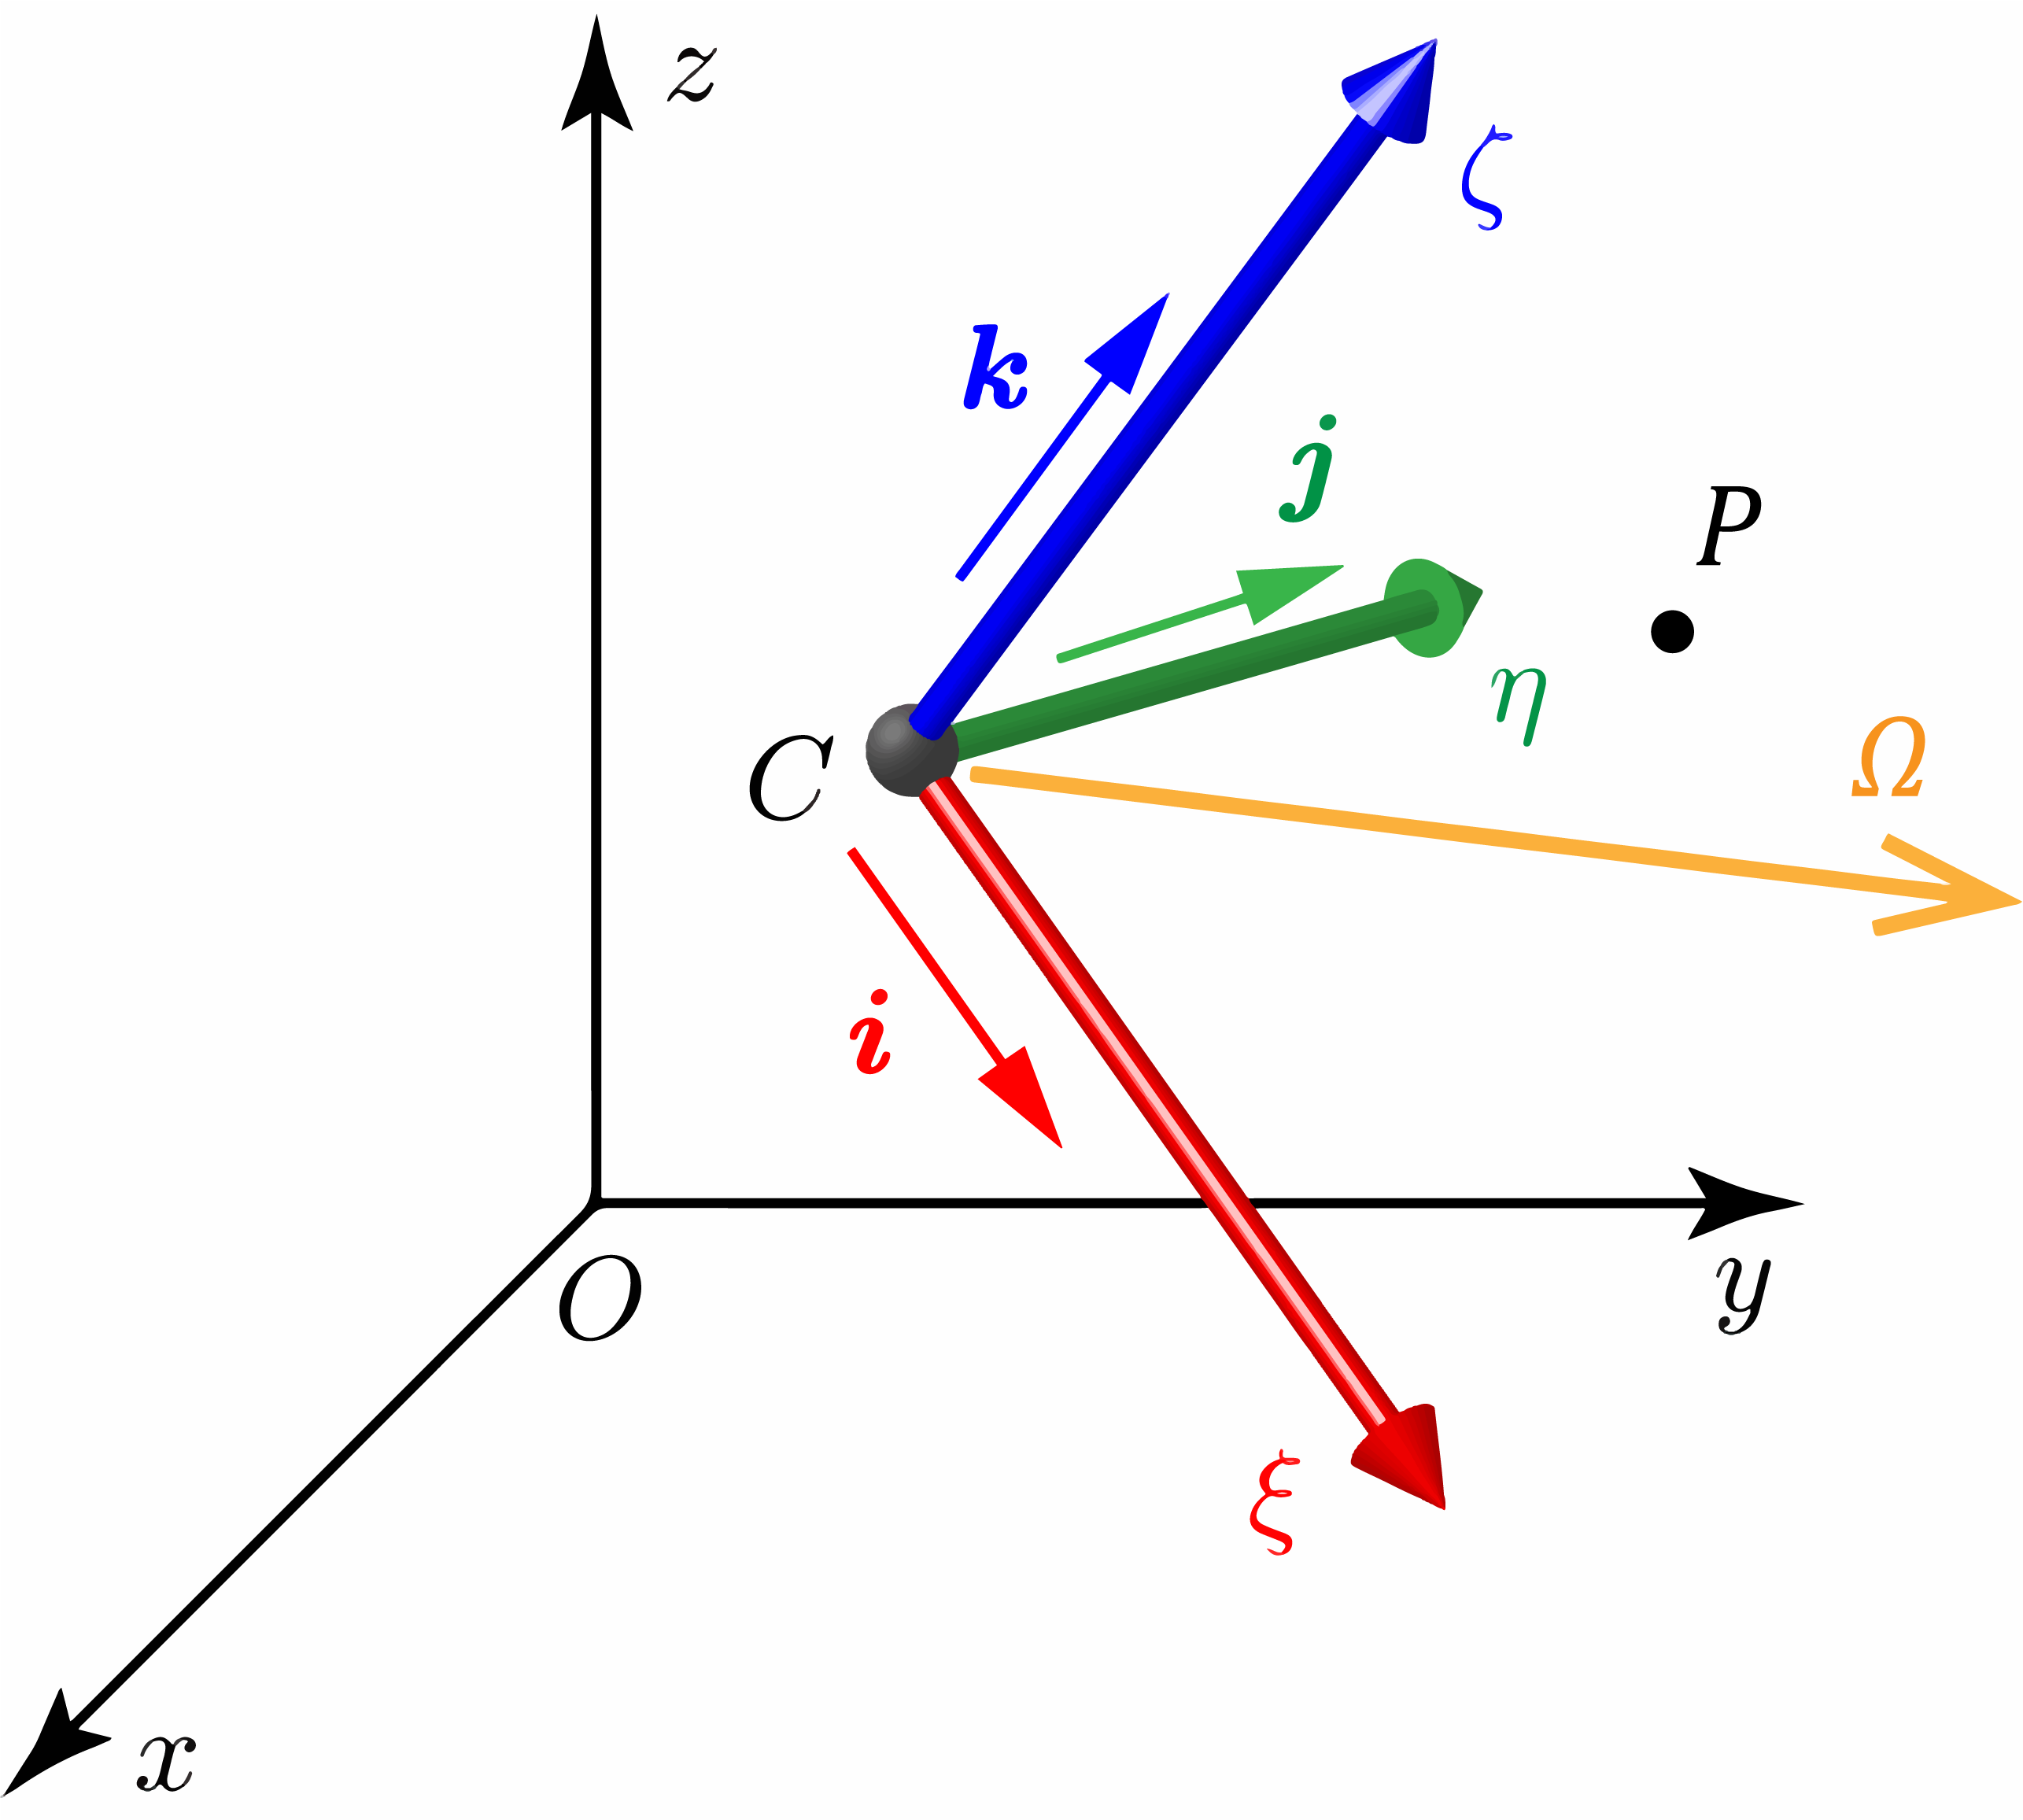
\includegraphics[width=6cm]{image/6-1-10.png}
\caption{参考系变换}
\end{wrapfigure}
第二点就是要给出新参考系的旋转角速度$\bs{\omega}$,\,角加速度记作$\bs{\beta}=\dot{\bs{\omega}}$.\,通过上一节我们知道,\,如果选取固连在新参考系的点$P$,\,并且把$\bs{CP}$记作$\bs{r}'$.\,那么$P$点速度加速度(现在记作$\bs{v}_c,\,\bs{a}_c$)为:
\[\bs{v}_c=\bs{v}_C+\bs{\omega}\times \bs{r}'\]
\[\bs{a}_c=\bs{a}_C+\bs{\omega}\times (\bs{\omega}\times\bs{r}')+\bs{\beta}\times\bs{r}'\]

我们现在研究什么问题呢?\,如果我们在$O-xyz$系中给出一个质点,\,也用$P$表示,\,的运动方程$x(t),\,y(t),\,z(t)$.\,其实也就给出了在$C-\xi\eta\zeta$系中的运动方程$\xi(t),\,\eta(t),\,\zeta(t)$.\,那么把位矢$\bs{OP}$记作$\bs{r}$,\,$\bs{CP}$记作$\bs{r}'$.\,再把$\bs{OC}$记作$\bs{r}_C$.\,于是得到恒等式:
\[\bs{r}=\bs{r}_C+\bs{r}'\]

但这不代表$\bs{v}=\bs{v}_C+\bs{v}'$.\,这里我们要注意有一点已经悄悄发生改变了,\,那就是导数,\,作为一个算符,\,变成了一个有多种自由定义余地的概念.\,只要想想这一点:\,从运动方程求出速度的过程叫做求导\footnote{导数就是从运动方程到速度矢量的映射},\,但是同一个运动方程对应的运动是同一个运动,\,但是在不同参考系中依然可以有多个不同的取值.\,这就足以说明有多种不同的求导方法.\,具体来说,\,这里的$\bs{r}'$可能有三种情况:\,a.\,固连在$C$系中,\,相对$C$系大小方向不变.\,b.\,相对地面系$O$系大小方向都不变,\,即$P$跟随$C$相对地面系平移.\,c.\,两者都不是.\,那么相应地定义三种导数:
\begin{enumerate}
	\item 绝对导数:\,即平常的$\displaystyle\frac{\ud}{\ud t}$,\,可以简单地用加点来代替.\,我们还创造一个新的符号$\uD$来表示求导,\,例如对于情形$b$,\,这个导数就是零.\,求导数的方法是:\,找到一个矢量在$O$系中每时每刻向三个坐标轴方向的投影分量并分别求导最后组合为矢量.\,用这个导数能定义$P$点在$O$系中的速度与加速度:
	\[\bs{v}=\uD \bs{r}(=\frac{\ud}{\ud t}\bs{r}=\dot{\bs{r}})\quad,\quad\bs{a}=\uD \bs{v} \]
	\item 相对导数:\,这就是要换相对$C$系的视角来研究一个矢量的导数了.\,我们记作$\uD'$.\,例如对于情形$a$,\,那么相对导数就是零.\,求导数的方法是:\,找到一个矢量在$C$系中每时每刻向三个坐标轴方向的投影分量并分别求导最后组合为矢量.\,这也就是说它用来定义相对速度和相对加速度是合适的:
	\[\bs{v}'=\uD'\bs{r}'=\dot{r_1'}\bs{i}+\dot{r_2'}\bs{j}+\dot{r_3'}\bs{k}\quad ,\quad \bs{a}'=\uD'\bs{v}'=\ddot{r_1'}\bs{i}+\ddot{r_2'}\bs{j}+\ddot{r_3'}\bs{k}\]
	\item 随体导数:\,这是矢量由于跟随$C$系转动而带来的相对$O$系的变化率.\,我们记作$\widetilde{\uD}$.\,例如在情形$a$中,\,$\bs{r}'$随体导数就是$\bs{\omega}\times\bs{r}'$.\,这个算符其实就等价于$\omega\times$,\,这是因为他就定义为:
	\[\widetilde{\uD}\bs{A}=A_1\bs{\ddot{\imath}}+A_2\bs{\ddot{\jmath}}+A_3\bs{\dot{k}}=A_1\bs{\omega}\times\bs{i}+A_2\bs{\omega}\times\bs{j
	}+A_3\bs{\omega}\times\bs{k}=\bs{\omega}\times(A_1\bs{i}+A_2\bs{j}+A_3\bs{k})=\bs{\omega}\times\bs{A}\]
\end{enumerate}

值得注意的是,\,这三个导数算符之间有如下关系:
\[\uD=\widetilde{\uD}+\uD'\]

这很容易证明,\,对一个矢量求导数,\,一看分量变不变,\,而看基矢量本身有没有旋转.\,那么就会产生两项.\,实际上就是莱布尼茨法则.

于是这才能推理参考系变换的公式.\,我们对$\bs{r}=\bs{r}_C+\bs{r}'$两边求绝对导数:
\[\bs{v}=\uD\bs{r}=\uD\bs{r}_C+\uD\bs{r}'=\bs{v}_C+(\widetilde{\uD}+\uD')\bs{r}'=\bs{v}_C+\bs{\omega}\times\bs{r}'+\bs{v}'\]

再次对上式两边求绝对导数:
\begin{align*}
\bs{a}=\uD\bs{v} &=\uD\bs{v}_C+\uD\bs{\omega}\times\bs{r}'+\bs{\omega}\times\uD\bs{r}'+\uD\bs{v}'\\
	  			 &=\bs{a}_C+\bs{\beta}\times\bs{r}'+\bs{\omega}\times(\widetilde{\uD}+\uD')\bs{r}'+(\widetilde{\uD}+\uD')\bs{v}'\\
	  			 &=\bs{a}_C+\bs{\beta}\times\bs{r}'+\bs{\omega}\times(\bs{\omega}\times\bs{r}')+\bs{\omega}\times\bs{v}'+\bs{\omega}\times\bs{v}'+\bs{a}'\\
	  			 &=\bs{a}_C+\bs{\beta}\times\bs{r}'+\bs{\omega}\times(\bs{\omega}\times\bs{r}')+2\bs{\omega}\times\bs{v}'+\bs{a}'
\end{align*}

这两个公式就是参考系变换下的变换公式:
\[\bs{v}=\bs{v}_C+\bs{\omega}\times\bs{r}'+\bs{v}'\]
\[\bs{a}=\bs{a}_C+\bs{\beta}\times\bs{r}'+\bs{\omega}\times(\bs{\omega}\times\bs{r}')+2\bs{\omega}\times\bs{v}'+\bs{a}'\]

如何理解以上的公式?\,事实上结构也很简单,\,我们把加速度中的最独特的一项单独拿出来叫做\emph{柯里奥利加速度}(Coriolis accelaration):
\[a_c'=2\bs{\omega}\times\bs{v}'\]

那么以上两公式具有以下结构:
\[\text{绝对}=\text{牵连}(+\text{柯氏})+\text{相对}\]

柯氏即柯里奥利.\,相对速度与相对加速度就是$\bs{v}',\,\bs{a}'$.\,言下之意就是我们定义了所谓的\emph{牵连速度}(convected velocity)与\emph{牵连加速度}(convected acceleration):
\[\bs{v}_c=\bs{v}_C+\bs{\omega}\times \bs{r}'\]
\[\bs{a}_c=\bs{a}_C+\bs{\omega}\times (\bs{\omega}\times\bs{r}')+\bs{\beta}\times\bs{r}'\]

细心的读者已经发现了,\,这两个式子和本节最开始推导出来的固连在$C$系中的点的绝对速度,\,加速度公式是一致的.\,牵连速度(加速度),\,顾名思义,\,被转动参考系``带着走''的速度(加速度).\,也正是以上规律启发我们总结出以下的动点动系法来理解看似复杂的速度加速度合成公式:
\begin{enumerate}
	\item 确定定系,\,动系,\,动点,\,定点.\,定系往往就是地面系;\,动系一般是相对某刚体或人为构造的刚性框架相对静止的参考系\footnote{注意,\,以下整个过程都可以脱离具体的坐标系而计算,\,这就为坐标系的选取(种类是直角坐标系,\,极座标系还是自然坐标系,\,方向如何)彻底提供了自由.};\,动点就是选做研究对象的相对两个系一般都有运动的点.\,最后,\,定点指的是这样的概念:\,在研究的一瞬间与动点重合,\,但是始终保持与动系固连的特殊参考点.
	\item 在定系考虑动点的运动.\,算出绝对量.\,在动系考虑动点的运动.\,算出相对量.\,在定系中考虑定点的运动,\,它的量就是牵连量.
	\item 建立绝对相对牵连之间的等量关系.
	\item 唯一要注意的是:\,只有当转动系是真转动的$\bs{\omega}\neq\bs{0}$,\,而且相对动系动点也是真运动的$\bs{v}'\neq\bs{0}$时,\,我们才有必要在加速度中添加一项柯氏加速度$2\bs{\omega}\times\bs{v}'$.\,从推导过程来看,\,一是即使固连在动系中的速度矢量也会跟随动系转动而带来加速度,\,二是动系中的相对位矢产生变化而带来在变化的牵连速度从而产生加速度,\,是造成柯氏加速度的两个因素.\,这一项不是因为在动系中的某特定位置而造成的,\,事实上与$\bs{r}'$无关,\,决定性因素是``相对动系有速度''.
\end{enumerate}

最后值得注意,\,如果$\bs{\omega}$和$\bs{\beta}$恒为零,\,这也并不少见,\,那么这样的动系就是\emph{平动系}(translational frame).\,此时公式极为简单,\,没有柯氏加速度,\,牵连量就是动系原点或任意固连点的量:
\[\bs{v}=\bs{v}_C+\bs{v}'\quad,\quad \bs{a}=\bs{a}_C+\bs{a}'\]

\subsection{刚体变换}

刚体的变换是点变换的直接推论.\,同样地,\,首先已知动系相对定系具有原点速度$\bs{v}_C$和加速度$\bs{a}_C$以及角速度$\bs{\omega}$和加速度$\bs{\beta}$,\,又已知定系中刚体基点速度加速度,\,现在记作$\bs{V},\,\bs{A}$.\,事实上我们还要给出刚体自己的角速度角加速度才算是对刚体的完整描述,\,它们为$\bs{\varOmega},\,\bs{B}$.\,那么绝对的和相对的各个量之间的关系为:
\[\bs{V}=\bs{v}_C+\bs{\omega}\times\bs{R}'+\bs{V}'\quad,\quad \bs{\varOmega}=\bs{\omega}+\bs{\varOmega}'\]
\[\bs{A}=\bs{a}_C+\bs{\beta}\times\bs{R}'+\bs{\omega}\times(\bs{\omega}\times\bs{R}')+2\bs{\omega}\times\bs{V}'+\bs{A}'\quad,\quad \bs{B}=\bs{\beta}+\omega\times\bs{\varOmega}'+\bs{B}'\]

证明过程留作练习由读者自己思考.

\section{运动的牵连}
最后本节旨在枚举一些在运动学解题中十分常见的初等模型与结论.

\subsection{接触系}
两个几何图形具有一个交点是一件非常常见的事情.\,交点将同时与两个几何图形保持结合关系.\,动态地看待这个问题,\,我们可以分别利用两个几何图形自身的运动和交点相对两者的运动合成来写出交点的速度矢量与加速度矢量来,\,但是作为同一个研究对象两种写法的结果理应相等.\,这构成了一组方程.

尤其是,\,在上述``相交系''中我们还有一类十分独特的情形,\,就是两个几何图形相切.\,两个平面形刚体如果始终保持相互接触,\,其轮廓之间就是这样的关系.\,此时要知道客观地这形除了一种约束:\,不是让两个刚体做任意运动都可以让两者保持相切的.\,所以必然存在所谓的\emph{约束方程}(equation of constraint).\,而这个方程的列法其实就是基于之前说的接触点的速度的一致性.

让我们看一个例子,\,它不仅帮助我们理解接触系,\,还可以帮助我们理解纯滚系.\,就是经典的在粗糙的地面上做匀速纯滚动的圆盘.\,首先应当注意到,\,涉及到所谓的``瞬时接触点''时可能指的是以下三个点之一:
\begin{wrapfigure}[8]{o}[-10pt]{7cm}
\vspace{0.1cm}
\centering
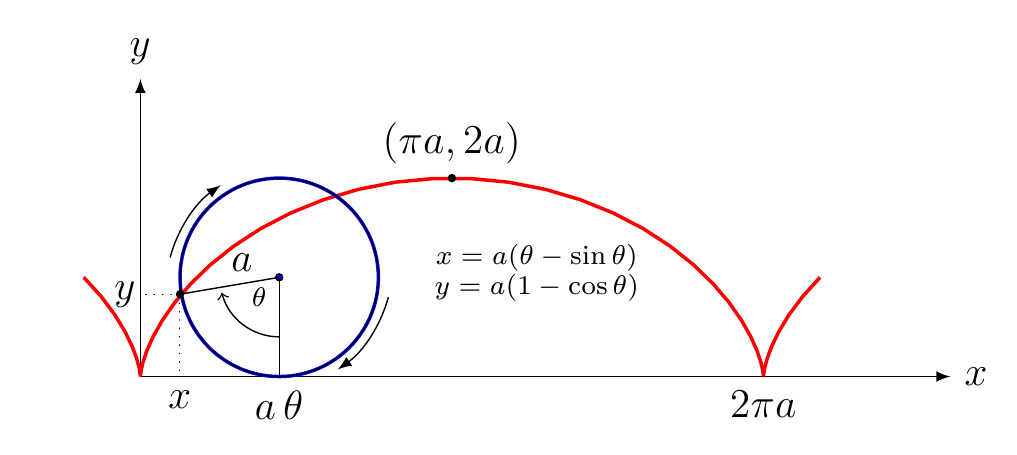
\includegraphics[width=7cm]{image/6-1-11.png}
\caption{圆盘在地面上做纯滚动}
\end{wrapfigure}

1.\,刚体1上的定点$P_1$.\,在这里取盘为刚体1,\,此时这个点是做旋轮线运动的那个点,\,此时恰好位于最低位置.

2.\,刚体2上的定点$P_2$.\,在这里取地面为刚体2,\,那么这个点就是一个静止的点.

3.\,动点$P_3$.\,就是每时每刻的切点形成的运动对象.\,在这里我们可以把圆盘变为圆筒,\,并且让一只松鼠在圆筒内部跑动以保持在最低位置,\,也就是每时每刻的切点.\,那么松鼠做匀速直线运动.

我们有什么结论呢?\,如果把$P_1$的瞬时速度在法线方向与切线方向的分速度与加速度写出来,\,分别是$v_{1n},\,v_{1\tau},\,a_{1n},\,a_{1\tau}$并约定法向以向刚体1内侧为正,\,切向可以以切线的任意一个方向为正.\,$P_2$同理为$v_{2n},\,v_{2\tau},\,a_{2n},\,a_{2\tau}$.\,那么让我们考虑一下$P_3$的速度与加速度.\,这就不难发现,\,如果采用动点动系法,\,就有:

速度:\,无论相对刚体1还是2,\,$P_3$的速度都是牵连加相对.\,牵连速度就是定点的速度,\,但相对速度由于点的轨迹就是刚体的轮廓,\,故方向必然在切线方向.\,然后由于速度的唯一性,\,这可以给出:
\[v_{1n}=-v_{2n}\]

加速度:\,道理是相同的,\,但需要注意两点,\,一是相对加速度具有了法线方向的分量.\,二是如果严格换一个刚体的转动系往往会带来柯氏加速度.\,具体解题时这仍然不失为一种常见的解题思路,\,但是难以总结现成的美妙,\,下一小节通过添加纯滚动这一更强的结论我们可以得到相应的方程.\,但是这个方程肯定是存在且可列式的,\,毕竟:

以上两个方程构成对接触系的约束的刻画.

\subsection{纯滚系}
上面的圆盘在地面上发生的运动实际上还是纯滚动.\,我们将首先给出纯滚动的定义,\,再来讨论纯滚动时的更强的附加条件,\,毕竟纯滚动相比简单的接触系还多一个约束.

事实上考虑相对运动就知道了,\,接触点在刚体1或2上相对运动的弧长就是相互滚动过的接触弧长,\,在两个刚体上应当具有公共值,\,这便是纯滚动的定义.\,这就是说:
\[\bs{v}_1'=\bs{v}_2'=\dot{s}\bs{\tau}\]

最后再利用$\bs{v}=\bs{v}_{1c}+\bs{v}_1'=\bs{v}_{2c}+\bs{v}_2'$.\,便得到了附加条件:
\[v_{1\tau}=v_{2\tau}\]

这就是常见的纯滚条件一,\,也就是说只有当相互接触的两个刚体定点切向速度一致才构成纯滚动.\,否则就是纯滚动的反面:\,必有相对滑动,\,俗称``连滚带滑''.

考虑加速度我们将得出一个不可思议但容易忽视的结论.\,首先注意到,\,如果两个刚体角速度分别为$\omega_1$和$\omega_2$,\,作为平面问题写成统一正方向的标量.\,而再设两刚体在接触点处轮廓的曲率为$k_1$和$k_2$.\,那么由于相对两刚体点在轮廓上的运动造成的单位时间切线方向的转角为:
\[\frac{\ud\theta_1}{\ud t}=\frac{\ud\theta_1}{\ud s}\frac{\ud s}{\ud t}=k_1\dot{s}\]
\[\frac{\ud\theta_2}{\ud t}=\frac{\ud\theta_2}{\ud s}\frac{\ud s}{\ud t}=k_2\dot{s}\]

而每当点成为切点两切线也会重合成为公切线,\,那么两个转角的和就是单位时间内两个刚体的相对转角:
\[\frac{\ud\theta_1}{\ud t}+\frac{\ud\theta_2}{\ud t}=|\omega_1-\omega_2|\]

最后,\,列出对刚体1和2牵连+柯氏+相对应当一致的方程:
\[a_{1n}-2\omega_1 \dot{s}+k_1\dot{s}^2=-(a_{2n}-2\omega_2\dot{s}+k_2\dot{s}^2)\]

整理得到纯滚条件二:
\[a_{1n}+a_{2n}=\frac{(\omega_1-\omega_2)^2}{k_1+k_2}\]

这是一个必然大于零的表达式\footnote{注意$k$本身可以小于零,\,但两个$k$的和必然大于零.},\,它意在,\,两个相接触的点必然后来会分离,\,这个分离加速度只与两刚体瞬时转动快慢和接触点弯曲程度有关,\,与平动转动加速度都没有关系.

\subsection{约束系}
约束是一种普遍存在且可以普遍讨论而有很广的适用范围的物理现象.\,本节并非要详细讨论约束,\,这一点在之后第三章静力学中再加以详细讨论.\,这里只讨论两个问题:\,绳系和杆系.

对于不可伸长的轻绳模型,\,如果它也被拉直(因为内部受力不为零又没有外力).\,那么在运动学层面上就等价于不可伸长的轻杆.\,设杆长为$l$,\,把两端点1和2速度加速度沿平行与杆与垂直与杆方向分解,\,具有关系:
\[v_{1\perp}-v_{2\perp}=\omega l\]
\[v_{1\parallel}-v_{2\parallel}=0\]
\[a_{1\perp}-a_{2\perp}=\beta l\]
\[a_{1\parallel}-a_{2\parallel}=-\omega^2 l\]

其中第二个关系就是著名的端点沿杆方向分速度必须是常数.\,对于绳子,\,即使绕过了定滑轮,\,显然沿定滑轮的切向速度也一直不变,\,因为绳子不可伸长.

最后,\,如果绳子允许弯曲但不允许伸长,\,其运动学约束方程该如何列?\,那就要求绳子上每一点在``局部''沿切向方向没有相对速度,\,表示为公式就是:
\[\frac{\ud \bs{v}}{\ud s}\cdot\bs{\tau}=0\]

注意这个条件不可以写为:
\[\frac{\ud v_\tau}{\ud s}=\frac{\ud (\bs{v}\cdot\bs{\tau})}{\ud s}=0\]

%%!TEX root = ../physical-olympics-2.tex
\chapter{动力学}


\section{牛顿定律}

\subsection{概述}
中世纪到近代以来物理学的发展,\,可谓沧海桑田,\,旧的观点被否定,\,几十年以后突然又以全新的面貌出现在物理学理论中.\,其中,\,实验中观察到各种令人惊诧的结果,\,无论物理学所依托的数学形式一变再变,\,要说亘古不变的主题,\,恐怕只有自然界的神奇与深邃,\,和我等凡人难以参透其中奥妙却仍为之孜孜不倦研究的决心.\,物理是一门研究自然界存在的运动并提出解释与理解方法的学科.\,运动形式多种多样,\,变化万千,\,但很多都被我们或多或少地解释,\,其实总结来看,\,从古至今我们也仅仅拥有过两类解释:\,一类由牛顿提出,\,一类则来自爱因斯坦.\,前前后后经历了大概以下发展:

\begin{description}
	\item[亚里士多德:]\, 天体运行,\,自由落体是自然(nature)的运动;\, ``树欲静而风不止''是强迫(violent)的运动.\,但错误地认为``物体越重,\,下落越快''
	\item[伽利略:]\, 辩证地看待亚里士多德的观点,\,开创性地提出相对性原理,\,成功论证与形成惯性与常见运动的正确认识.
	\item[笛卡尔,\,惠更斯等:]\, 成功得到大量动力学公式,\,包括后来的牛顿第二定律,\,动能的表达式与能量守恒定律,
	\item[牛顿开创的相互作用观:] \, 开创性的提出物质间存在相互作用,\,相互作用是改变物质运动状态的原因.\,并很好地把天体的运动归结到互相之间产生的相互作用上.\,后人建立了场的理论以后,\,超距的粒子间相互作用就不再被理论学家们采纳了,\,而要理解为场与粒子的相互作用,\,再晚一点,\,场和粒子都被赋予了波粒二象性,\,粒子也要被理解为场,\,但所有场都要被被分解为平面波,\,平面波又要被量子化.\,如果没有相互作用,\,那么这些平面波的运动状态就不会发生改变,\,只有相互作用才会改变其运动,\,或传播方向发生偏折(发生散射),\,或强度发生改变(粒子的产生与湮灭).\,牛顿的观点是以\emph{相互作用}(interaction)为核心的观点.
	\item[拉格朗日,\,哈密顿等:]\, 将牛顿的结果与观点上升到\emph{分析力学}(analytic mechanics)的高度.\,将复杂体系的结构浓缩在统一的一个能量函数或作用量泛函数中.\,为后来场论建立和相对论,\,统计力学,\,量子力学的发展都提供了理论支持.
	\item[马赫:]\, 批判牛顿的过于绝对的时空观.\,预言质量分布会对惯性本身产生影响.
	\item[爱因斯坦开创的几何观:] \,  仿佛又回到了亚里士多德,\,不仅仅是无相互作用下的匀速直线运动,\,一切在万有引力下的天体运动其实也是``自然''的运动.\,看上去复杂的曲线运动不过也是沿对被引力所扭曲的弯曲时空几何下的天然``直线''---测地线(geodesic)运动而已.\,对引力问题提出开创性的解释.\,率先描绘了20世纪建立的若干理论的物理图像.
	\item[天体物理,\,粒子物理:]\, 爱因斯坦以后的理论研究中很多问题还处于开放状态.\,时而采用牛顿的相互作用观,\,时而采用爱因斯坦的几何观.\,是一种两个图像的有机结合.
\end{description}

我们今天说\emph{经典力学}(classical mechanics)大多数情况即指\emph{牛顿力学}(Newtonian mechanics),\,指的是由伽利略最初引领,\,笛卡尔,\,惠更斯等奠基,\,牛顿集大成的一套理论.\,它以伽利略的\emph{两种新科学的对话与数学展示}(Discorsi e dimostrazioni matematiche intorno a due nuove scienze)和牛顿的\emph{自然哲学的数学原理}(Philosophi\ae\ Naturalis Principia Mathematica)两篇文献为核心.\,逻辑上以质点的牛顿三大定律为基础.\,不包括后来上升到的分析力学层次,\,作为绝对时空观适用伽利略变换,\,不兼容相对论.

牛顿定律总结如下:
\vspace{0.5cm}

\hrule
\begin{enumerate}
	\item 第一定律:\quad 在惯性系中,\,一个质点应静止或匀速直线运动.\,除非有外力施加于物体.
	\item 第二定律:\quad 在惯性系中,\,质点受力的矢量和$\bs{F}$等于其质量$m$与加速度$\bs{a}$的乘积.
	\item 第三定律:\quad 一个质点对另一个质点施加作用力时,\,另一个质点同时将施加反作用力于第一个质点,\,作用力与反作用力等大反向共线.
\end{enumerate}
\hrule
\vspace{0.5cm}

三个定律之间的联系是很值得讨论的.\,对三个基本定律的设置反映了很多物理思想\footnote{例如爱因斯坦狭义相对论的两个假设在某种意义上与牛顿第一第二定律的逻辑完全一致.\,都是先定义时空背景再阐述物理规律的共性.}.\,分析如下:

\subsection{牛顿第一定律}
牛顿第一定律旨在阐述时空的平直性.

也正基于以上这一点,\,我们不能仍为牛顿第一定律可以由牛顿第二定律出发推导.\,它不是表面上的牛顿第二定律中$\bs{F}=\bs{0},\,\bs{a}=\bs{0}$的特例.\,恰恰相反,\,即使从形式上看,\,也应当先由牛顿第一定律给出\emph{惯性系}(inertial frame)的概念才能适用牛顿第二定律.\,那么怎样的参考系是惯性系呢?\,牛顿第一定律是暗含认可\emph{绝对惯性系}(absolute inertial frame)的存在性的.\,在这样第一个系中牛顿第一定律才可以成立.\,这一个系无非就是由某种特殊运动状态的观察者(绝对观察者)建立的三维欧几里得空间坐标系外带一维时间坐标.\,而只要质点不受力(力是对相互作用的描述,\,只要远离其它所有物质就会使质点成为\emph{孤立}(isolated)的),\,就会静止或匀速直线运动,\,所谓匀速直线运动是指:
\[\begin{pmatrix}x(t)\\y(t)\\z(t)\end{pmatrix}=\begin{pmatrix}x(0)\\y(0)\\z(0)\end{pmatrix}+\begin{pmatrix}v_x\\v_y\\v_z\end{pmatrix}\cdot t\]

其中三个速度$v_x,\,v_y,\,v_z$都是常数.\,但是我们发现,\,相对这个系做匀速直线运动的另一个无自转观察者建立的系中,\,原来做匀速直线运动的质点现在依然做匀速直线运动.\,所以这样的系也叫做惯性系,\,可以叫做相对惯性系.\,即:\,惯性系就是任何相对绝对惯性系做匀速直线平动的参考系.\,而惯性系就是牛顿定律成立的前提条件.

所以牛顿的经典力学体系的第一大特点是承认绝对惯性系的存在性.\,实际上承认这一点也几乎等价于承认了时空的平直性.\,只不过在众多彼此等价(任何物理实验都不足以判断这些系的不等价性)的系中,\,牛顿认为还应当有一个第一性的,\,``最初''的惯性系.

\subsection{牛顿第二定律}
牛顿第二定律是牛顿定律的核心,\,旨在描述相互作用对运动的影响.

\emph{相互作用}(interaction)是牛顿经典力学后经过了几百年发展而浓缩出来的更普遍的概念.\,如果没有相互作用,\,物质基本的运动模式就是``惯性''的,\,如匀速运动的粒子或传播的平面波.\,任何使物质偏离这种``惯性''运动的模式的原因就都在相互作用上.\,相互作用的模式是多种多样的,\,除了牛顿指出的下面仔细讨论的情形,\,光会因为与物质相互作用而产生吸收和散射,\,两个惰性气体原子靠近时两个电子云也会产生量子的诱导极化而使原子间产生范德瓦耳斯吸引.\,这些都是广义的相互作用,\,但是为了描述它们,\,前者需要借助波来描述光这种物质,\,后者还需要借助波函数来描述电子云,\,相互作用更是要依赖于薛定谔方程等来理解.\,所以经典物理理论有它的适用性,\,这一点在下面我们需要记住.

这也就是牛顿经典力学体系的第二大特点了:\,物质的基本模型一律视作\emph{质点}(mass point)\footnote{牛顿甚至认为光也适用于质点模型},\,相互作用的基本模型一律视作\emph{力}(force),\,质点具有惯性这一基本属性,\,用\emph{质量}(mass)来描述.

从牛顿第二定律$F=ma$形式上看,\,难免会由于数学思维得出``用力来定义质量的多少''或者是``用质量定义力的大小''这样的观点,\,而进入力与质量循环定义的误区.\,但实际上谁也没有定义谁.\,因为正常的物理思维是先要提前定义质量和力:

首先质量是受力物体所固有的属性之一,\,它具有广延性:\,如果把质量为$m_1$的质点与质量为$m_2$的质点复合为一个大质点,\,其质量变为$m_1+m_2$.\,可比性:\,任意两个质点的质量都可以依照在同样大小的力下的行为来比较其质量的比例关系\footnote{事实上用碰撞实验可以给出一个更简单的比较质量的方法,\,让待测质量的质点以一个单位的速度去正碰撞一个以$x$个单位速度运动的单位质量的质点,\,若恰好停下就说明待测质量为$x$个单位质量,\,若没停下就改变$x$的值直到停下.}.\,和固有性:\,只要质点没有变性,\,质量就不变,\,所以在不同参考系去看同一个质点,\,在运动的不同时刻质量都是严格不变的,\,也称``质量守恒'',\,我们将避免这一称呼,\,因为一般的守恒量只是针对一个参考系中的过程中的各个状态,\,而换一个系看守恒量往往要变,\,质量却显然不变,\,这是其一;\,另外相对论下质量就不再守恒了,\,它不普遍,\,这是其二.

力也是对固有的相互作用的强度做的描述.\,它也是固有的,\,应当有一种合理的公式去描述施力物体的状态如何影响施加的力(这个力也与受力物体的状态有关).\,而且如果换一个参考系考虑,\,力的强度是不变的.\,根据力对质点产生的效果,\,力也应当具有矢量性,\,不同两个力是可以比较的,\,很多情况下甚至可以叠加:\,多个施力物体互不影响各自施加的力,\,同时作用于同一个受力物体,\,在生活中这种现象非常常见,\,不难得出这样的总结.

于是才有了牛顿的著名论断:
\[\bs{F}=m\bs{a}\]

这样一个定律内容是丰富的,\,它首先是兼容于伽利略相对性原理从而自洽:\,在另外的惯性系中考察,\,$F$和$a$都是不变的.\,但是又不是兼容于相对性原理的唯一解决方案,\,狭义相对论,\,就提供了另一套可能性,\,在低速极限$v\ll c$时狭义相对论的动力学方程表达式和这并无二致;\,其次质量$m$作为系数联系了力(原因)与加速度(结果)这并不是偶然,\,它也是为了和叠加原理相协调:\,一份的力作用在一份质点上产生这样的加速度,\,那么把两份力各自作用在两份质点上那就还是产生同样的加速度.\,所以力除以质量决定运动学加速度\footnote{即$F/m=f(v,\,a)$}那是天经地义.\,至于为什么两份力作用在原来的一份质点上会产生加速度加倍的效果,\,这就是经典力学中的类似于公理性质的存在了.

\subsection{牛顿第三定律}
牛顿第三定律是对``相互作用''中的``相互性''的刻画,\,暗示了动量与角动量守恒.

任何物理理论,\,如果妄想在短短几条式子中道尽万千世界发展与变化的规律,\,都是玄学而不是科学.\,科学的精神是要基于事实,\,进行总结与归纳,\,借助数学进行基本的抽象与再创造.\,所以现实就是,\,世界的运行本就是复杂的,\,不可预测的.\,物理学的发展史也就充满了惊人的转折:\,每当人们以为在某一个大的领域有简单而清晰的图像共识的时候,\,总是会有意外发生告诉人们特殊情况下理论不再适用.\,原则上,\,没有任何命题能够成为物理学上的公理:\,它能无条件适用于从宇观到微观的方方面面.

牛顿清楚地意识到了物质与物质之间相互作用的复杂性,\,是不可能用几个简单的公式写出所有情况下他的理论中两个任意质点之间的作用力的.\,所以退而求其次,\,用牛顿第三定律来描述了所有情形下这样的力需要满足的条件.\,的确合情合理.\,但是又看牛顿第三定律的提法本身是否合理?

实际上我们先注意到动量守恒和角动量守恒的条件比牛顿第三定律的条件要强(也更本质):\,我们可以由前者推导出后者.\,以动量为例,\,动量是用来描述一个体系的动力学运动趋势的.\,动量守恒就意味着,\,如果一个孤立的体系的一部分``平均地''在初始时刻具有向前运动的趋势,\,比如一部分向前运动而另一部分静止.\,那么之后就绝对不可能演化为向后运动.\,或者还可以这么理解:\,如果看到一个质点在做一个非匀速直线运动:\,比如忽快忽慢的直线运动,\,那么显然单独看质点本身动量并不守恒.\,但是这必然意味着质点不是孤立的,\,必须和别的体系一同看作一个整体,\,质点增加或减少的动量必须由体系的另一部分的动量减少或增加来抵消,\,来满足整体动量守恒的需求.\,如果体系仅仅由两个质点构成,\,再把动量的增加或减少的快慢理解为受力(动量定理),\,我们就有了牛顿第三定律中关于相互作用力等大,\,反向的部分.

所以动量守恒可以用来``证明''牛顿第三定律中的一对相互作用力.\,同理角动量守恒则可以用来证明牛顿第三定律中质点间相互作用力共线的部分.\,最后读者可以验证牛顿第三定律的数学形式为\footnote{$\bs{F}_{12}$表示1给2的力.}:
\[\bs{F}_{12}+\bs{F}_{21}=\bs{0}\quad,\quad \bs{r}_2\times\bs{F}_{12}+\bs{r}_1\times\bs{F}_{21}=\bs{0}\]

之所以这么理解是因为,\,动量守恒和角动量守恒显得更普适.\,事实上,\,它们是体系物理规律在空间平移对称性和旋转对称性下具有协变形式的直接推论.\,这一点是由近代著名的\emph{诺尔特定理}(Noether Theorem)这一数学定理精确证明了的.

也正是牛顿第三定律暗示了牛顿经典力学体系的缺点.\,因为我们无法解释牛顿第三定律的``自然性'',\,取消牛顿第三定律所构成的体系无非是具有外力的非孤立系(动量不守恒),\,牛顿第三定律为体系增添的``结构性要求''并没有很好地由理论解释与包含.\,所以才有了后来建立在对守恒量,\,尤其是能量进行强调的分析力学理论的提出.

\subsection{质点系与它的牛顿定律}
对于复杂体系,\,牛顿提出一种可能的等效观点,\,就是把任意这样的体系看做是一种离散的质点系的推广.\,质点系由质点集合$\{(m_i,\,\bs{r}_i)\},\,(i=1,\,2\,\cdots \,n)$组成.\,我们只要找到从质点理论到有限质点构成的质点系理论中那些不变的结论,\,就有理由相信这些结论可以推广到复杂的真实体系.\,因为真实体系被期待可以用一个足够大数目的质点系来近似.\,对于复杂的质点系首先需要引入\emph{质心}(center of mass,\,{\rm CM})的概念:
\[\overline{\{(m_i,\,\bs{r}_i)\}}=(m_C,\,\bs{r}_C)\]

我们的做法是:\,直接把质心理解为一个新的质点,\,它具有新的质量$m_C$和位置$\bs{r}_C$,\,并满足表达式:
\[m_C=\sum_i m_i\quad;\quad \bs{r}_C=\frac{\sum_i m_i\bs{r}_i}{\sum_i m_i}\]

可以把上式读作:\,质心的质量等于质点系的总质量,\,质心的位矢是各个质点位矢关于质量的加权平均.

质心的求法是符合交换律与结合律的.\,这在质量上是显然的,\,因为质心质量就是各个质点质量构成的连加式.\,对于质心位矢,\,考虑总质量为$m_1$的第一个质点系$(m_{1i},\,\bs{r}_{1i})$和总质量为$m_2$的第二个质点系$(m_{2j},\,\bs{r}_{2j})$复合而成的整个质点系,\,如果直接算两个体系质心形成的质心:
\[\frac{m_1\bs{r}_{1C}+m_2\bs{r}_{2C}}{m_1+m_2}=\frac{\displaystyle\sum_i m_{1i}\cdot \frac{\displaystyle\sum_{i} m_{1i}\bs{r}_{1i}}{\displaystyle\sum_i m_{1i}}+\displaystyle\sum_j m_{2j}\cdot\frac{\displaystyle\sum_{j} m_{2j}\bs{r}_{2j}}{\displaystyle\sum_{j} m_{2j}}}{\displaystyle\sum_i m_{1i}+\displaystyle\sum_j m_{2j}}=\frac{\displaystyle\sum_{k\in 1\& 2}m_k\bs{r}_k}{\displaystyle\sum_{k\in 1\& 2}m_k}\]

可以发现这就是整个体系的质心.\,这种方法就是``组合法'',\,比如求几根棍子的质心,\,可以把棍子替换为在质心的质点再求.\,由此还可以引申出``割补法''或者``负质量法'',\,不过就是把上式反过来理解:\,如果我们要求第一个体系的质心,\,不难验证可以这样求:
\[\bs{r}_{1C}=\frac{m\bs{r}_C-m_2\bs{r}_{2C}}{m-m_2}\]

动态地看待求质心的式子,\,还可以发现,\,求导以后,\,我们得到了质心作为一个在运动的质点,\,其速度,\,加速度也是可以直接从原质点系来做加权平均的:
\[\bs{v}_C=\frac{\sum_i m_i\bs{v}_i}{\sum_i m_i}\quad;\quad \bs{a}_C=\frac{\sum_i m_i\bs{a}_i}{\sum_i m_i}\]

为了推导出质点系的类似的牛顿定律,\,我们发现牛顿三大定律是缺一不可的.\,当然原则上如果没有牛顿第三定律,\,我们就把作用在每一个质点$m_i$上的合力,\,不管施力物体是谁,\,记作$\phantom{}^tF_i$,\,``t'' for ``total''.\,原则上我们也可以得到:
\[\phantom{}^t\bs{F}=\sum_i m_i\bs{a}_i\quad \phantom{}^t\bs{F}=\sum_i\phantom{}^t\bs{F}_i\]

这一点很容易证明,\,只需要把每个质点的牛顿定律加起来即可.\,但是注意到牛顿第三定律既然正确,\,我们就可以做进一步的研究:\,把任何质点受力分解为\emph{内力}(internal force)和\emph{外力}(external force):
\[\phantom{}^t\bs{F}_i=\phantom{}^{in}\bs{F}_i+\phantom{}^{ex}\bs{F}_i\]

内力指$i=1,\,2\,\cdots\,n$个质点之间一对一对存在的力,\,所以实际上不如写明:
\[\phantom{}^{in}\bs{F}_i=\sum_{j\neq i}\bs{F}_{ji}\]

最后单独的那个真正的外力以后直接简写为$\phantom{}^{ex}\bs{F}_i=\bs{F}_i$.

经过这么一番折腾完以后,\,我们还是把所有质点的牛顿定律来求和,\,但是注意到由于牛顿第三定律关于相互作用力等大反向的部分,\,内力相互抵消,\,得到:
\[\bs{F}=\sum_i m_i\bs{a}_i\quad \bs{F}=\sum_i \bs{F}_i\]

这就是质点系的牛顿第二定律,\,相比上面那个也对的直接把每个牛二加起来的表达式,\,能引起注意的变化只有一点,\,那就是:\,不需要考虑内力!\,但正是这一点极大地简化了很多实际问题的分析.

值得一提,\,我们顺理成章地要考虑另外两个层面的规律,\,一是``对质心'',\,二是``相对质心''.\,前者值的是,\,把质心作为一个质点来研究问题.\,那么问题也很简单,\,利用之前证明过的:
\[\bs{a}_C=\frac{\sum_i m_i\bs{a}_i}{\sum_i m_i}\quad \Rightarrow \quad m_C\bs{a}_C=\sum_i m_i\bs{a}_i\]

就可以得到:
\[\bs{F}=m_C\bs{a}_C\]

这就是著名的\emph{质心运动定律}(motion law of {\rm CM}).\,特殊的,\,如果合外力$\bs{F}=\bs{0}$.\,那么退化到\emph{质心守恒}:\,质心做匀速直线运动或者静止.

最后我们提出质心系的概念.\,\emph{质心系}(frame relative to {\rm CM})指:\,原点在质心的平动欧几里得坐标系.\,结合我们已经学过的和将来要学的所有内容我们把其性质罗列如下,\,请读者能够给出证明的直接证明,\,给不出的带着问题往下学习:
\begin{itemize}
	\item 质心系虽然有非惯性力,\,但非惯性力与原力系主矢和为零.
	\item 质心系虽然有非惯性力,\,但非惯性力系对质心的主矩为零.
	\item 质心系是零动量系.
	\item 质心系虽然有非惯性力,\,但非惯性力在过程中总功和为零.
	\item 取质心为原点能使质点系二阶矩最小,\,故刚体相对所有平行轴中以过质心的轴转动惯量最小.
	\item 只有取质心才能写出柯尼希定理.
\end{itemize}

\subsection{非惯性系的处理}
虽然牛顿定律只在惯性系中成立.\,但是如果我们选取一个相对惯性系的转动系,\,其原点速度加速度为$\bs{v}_C$与$\bs{a}_C$.\,而角速度与角加速度分别为$\bs{\omega}$与$\bs{\beta}$.\,本来在原来的惯性系中研究一个质点,\,正确的式子是:
\[\bs{F}=m\bs{a}\]

现在换了参考系以后,\,将不能仿照上式写出一个依然正确的式子.\,但是加速度变换总是对的:
\[\bs{a}=\bs{a}_C+\bs{\beta}\times\bs{r}'+\bs{\omega}\times(\bs{\omega}\times\bs{r}')+2\bs{\omega}\times\bs{v}'+\bs{a}'\]

而我们也永远认为力矢量在参考系变化下是大小与方向都不变的:
\[\bs{F}=\bs{F}'\]

代入就足以得到依然正确的,\,仅仅用新的非惯性系中的各个参量表示的类牛顿定律.\,我们以后将直接叫做非惯性系中的牛顿定律:
\[\bs{F}'+(-m\bs{a}_C)+(-m\bs{\beta}\times\bs{r}')+[-m\bs{\omega}\times(\bs{\omega}\times\bs{r}')]+(-2m\bs{\omega}\times\bs{v}')=m\bs{a}'\]

可以发现,\,这类似于需要为质点运动虚构一些力,\,它们全都称作\emph{惯性力}(force of inertial).\,包括:
\begin{itemize}
	\item 平动惯性力$-m\bs{a}_C$,\,典型的情况就是平动而非转动的非惯性系中的惯性力.\,特点是一个恒力,\,而与质点的运动状态无关.
	\item 切向惯性力$-m\bs{\beta}\times\bs{r}'$与惯性离心力$-m\bs{\omega}\times(\bs{\omega}\times\bs{r}')$,\,典型的情况是绕轴做旋转的参考系.\,特点是这两个力仅仅依赖于质点的位置,\,离轴越远力越大,\,在轴上力就消失了.
	\item 柯里奥利力$-2m\bs{\omega}\times\bs{v}'$,\,典型的情况是相对转动系还有运动的情况.\,特点是给出一个与位置无关,\,但是正比与速度大小,\,方向始终垂直于速度方向的力.
\end{itemize}

如果我们的研究对象是一个刚体而非质点,\,那么相当于每一个质点上都要受到不同的惯性力.\,此时如果考虑这些所有力作用在刚体上的等效合力和力矩,\,那么将是一个非常复杂的情况,\,尤其是,\,各个柯里奥利力将对刚体整体造成所谓的``回转力矩'',\,用这个观点可以解释很多第七章刚体中的现象,\,感兴趣的读者可以参考相关资料.

\section{动量定律}
这四节我们将罗列质点与质点系动力学的核心内容.\,读者应当具有初等的牛顿理论的基础.\,这一部分与三个牛顿定律的关系如何?\,首先它们是牛顿定律的自然延伸,\,属于并占据经典力学的主要部分.\,其次这些结论与相关推论适用性很强.\,比如三个守恒律:\,动量能量与角动量的守恒几乎是在所有物理理论中普适的.\,从内容上看关于质点系的定律自然就包含了单质点的相应特殊情况.\,而写法总是有三种:\,相对地面系的,\,相对质心系的和把质心作为质点的.\,联系三种写法的是质心系独有的各个柯尼希定理.\,最后,\,能量比较特殊我们单独列一小节多加阐述,\,具体的碰撞问题加一节,\,最后再补充一个新的位力定律.\,便构成了一$3\times3$条定律为主干的本章的内容.\,实际上也就是牛顿经典力学的核心部分.

\subsection{质点的动量}
质点的\emph{动量}(momentum)定义为:
\[\bs{p}=m\bs{v}\]

很直接地可以推导出质点的\emph{动量定理}(law of momentum)来,\,用$\bs{F}$表示合力:
\[\bs{F}=\frac{\ud \bs{p}}{\ud t}\]

证明过程就是把牛顿定律右侧拿来等量代换.

质点动量守恒并不是守恒律最常见的提法.\,但是不管怎样,\,我们能看出来,\,如果在某方向\footnote{必须是直角坐标!\,比如极坐标下$F_\theta=0$但$p_\theta$不守恒,\,$L=rp_\theta$才是对应的守恒量,\,个中缘由涉及到分析力学.}分力为零,\,那么该方向分动量导数为零,\,从而是一个不变量.

\subsection{质点系的动量}
依据上一节的符号约定,\,质点系$\{m_i,\,\bs{r}_i\}$中第$i$个质点的牛顿定律写作:
\[\bs{F}_i+\sum_{j\neq i}\bs{F}_{ji}=m_i\bs{a}_i\]

所谓质点系的动量定理,\,无非就是把上式拿去对每一个质点求和,\,然后等号右侧化为动量的形式.\,过程中我们发现需要定义:

质点系的总动量:
\[\bs{p}=\sum_i \bs{p}_i=\sum_i m_i\bs{v}_i\]

外力矢量和:
\[\bs{F}=\sum_i \bs{F}_i\]

过程中内力全然抵消,\,这就导致了最后表达式简单地为:
\[\bs{F}=\frac{\ud \bs{p}}{\ud t}\]

\vspace{0.5cm}

接下来就是研究质心的两个层次,\,一是把质心作为质点研究等号左侧的``作用''和等号右侧的``动力学量'';\,二是考虑相对质心系的引入惯性力以后的新写法.

如果在地面系中质点系受到一个力$\bs{F}_\alpha$,\,那么把这个力移动到质心上以后,\,我们认为这个力是不需要改变的.\,但是如果考虑相对质心系,\,固然原来的力也是存在且不变,\,但是还得考虑惯性力.\,那么总的合力推导出来应当是:
\[\bs{F}_C=\bs{F}\quad ,\quad \bs{F}'=\bs{0}\]

后者是因为惯性力的合力$\displaystyle\sum_i -m_i\bs{a}_C=\sum_i -m_i\bs{a}_i=-\bs{F}$.\,我们发现有:
\[\bs{F}=\bs{F}_C+\bs{F}'\]

形如上式的式子都可以叫做\emph{柯尼希定理}(K\"onig theorem).\,再来看动量,\,质心动量就应当是质点系总动量,\,而相对质心系动量必然为零:
\[\bs{p}_C=\bs{p}\quad,\quad \bs{p}'=\bs{0}\]

前者由于质心的定义很容易看出来,\,后者一般被叫做:\,质心系是零动量系,\,两者之和符合:
\[\bs{p}=\bs{p}_C+\bs{p}'\]

这就不难看出:
\[\bs{F}_C=\frac{\ud \bs{p}_C}{\ud t}\]
\[\bs{F}'=\frac{\ud \bs{p}'}{\ud t}\]

最后我们讨论普遍的\emph{动量守恒}(conservation of momentum).

第一,\,动量守恒是普遍的,\,虽然表面上看$\bs{F}=\dfrac{\ud\bs{p}}{\ud t}$一个体系的动量只要外力不为零就会有非零的导数.\,但是根据动量守恒的精神,\,一个体系的动量增必然以另一个体系动量的减为代价,\,也就是需要注意到既然存在外力$\bs{F}$,\,那就需要考虑力作用的相互性.\,只要把所有施力物体都归入同一个体系使相互作用封闭.\,那么等号左侧只能是零,\,那么等号右侧就会有普遍的动量守恒.

第二,\,有些场合动量不以质点为载体而是以场为载体.\,动量依然守恒,\,毕竟我们将认为场给质点的力与``质点给场的力''构成反作用力符合牛顿第三定律.\,事实上只要可能涉及到超距作用就一定是要用场来处理的,\,不用场处理可能导致不精确甚至谬误的结果,\,这是因为牛顿第三定律都不一定适用.\,只要想想一个质点位置突然改变,\,由于相互作用传递速度必然有限导致相隔一定距离的第二个质点受力变化将会延迟,\,就不能使得这个力等于同一时刻的反作用力,\,那么两质点的动量和就不再守恒.\,另一种典型的情况是两个电流元之间的磁场安培力也不符合牛顿第三定律,\,全都是因为有场的动量未计入计算的缘故.\,所以这些场合,\,如果牛顿第三定律``近似''适用,\,我们才说质点系的动量``近似''守恒.\,严格的动量守恒设计场论的知识,\,有兴趣的读者可以进行相关学习.


\section{角动量定律}

角动量的逻辑与上一节是完全一致的.\,只不过在牛顿定律的数学处理上要多一步罢了.

\subsection{质点的角动量}
选取一个参考系的原点$O$以后便可以写出质点的位矢$\bs{r}$.\,那么质点受力对$O$的\emph{力矩}(moment of force,  moment, torque)定义为:
\[\bs{M}=\bs{r}\times\bs{F}\]

而为质点则定义一个动力学量也就是\emph{角动量}(angular momentum):
\[\bs{L}=\bs{r}\times \bs{p}=\bs{r}\times m\bs{v}\]

之所以这么做,\,一种想法是对牛顿定律$\bs{F}=m\bs{a}$两侧用$\bs{r}$叉乘的一种可能的构造思路\footnote{Noether定理才是严谨的构造思维.}.\,这就能给出\emph{角动量定律}(law of angular momentum):
\[\bs{M}=\frac{\ud \bs{L}}{\ud t}\]

证明过程只消注意到右边莱布尼茨法则出来两项的另一项$\dot{\bs{r}}\times\bs{v}=\bs{v}\times\bs{v}=\bs{0}$.

角动量定律有一个值得注意的点,\,那就是\emph{矩}(moment)的中心的选取的任意性.\,角动量(动量的矩)和力矩都因为是$O$点计算的才具有位矢$\bs{r}$,\,这个点叫做\emph{矩心}(center of moment).\,而选取不同的矩心的结果就会产生不一样的定律的表达式形式,\,它们都是对的.\,但是解题时何以选取?\,这个复杂的问题我们下一章再做简要介绍.

另一个点是原则上必须选取不动的点作为矩心.\,选取动点暗含两层意思,\,一是,\,可能需要把每一个粒子对动点的动量理解为相对速度对应的动量.\,二是,\,可能在求角动量的导数时要求的是跟随动点的角动量的导数.\,无论哪一点都将使得相应结论不再正确.\,当然,\,如果两种可能的更改都没有发生,\,即,\,仅仅是这一时刻对这一点列瞬时的角动量定律,\,下一时刻换下一个点列.\,那么这就是构成一个时时刻刻都成立的等式,\,只有在这种意义下角动量定律才可以原封不动地应用.\,否则需要重新从牛顿定律出发加以推导.

质点的角动量守恒也不是一个典型的结论.\,但是有一种典型的情形:\,就是平面上一个有心力作用下的质点运动是角动量总是守恒的.\,因为此时$\bs{F}\parallel \bs{r}\;\Rightarrow\;\bs{M}=\bs{0}$.

\subsection{质点系的角动量}

定义质点系的总角动量:
\[\bs{L}=\sum_i\bs{L}_i=\sum_i\bs{r}_i\times m_i\bs{v}_i\]

外力力矩和(不需要包括内力):
\[\bs{M}=\sum_i\bs{M}_i=\sum_i \bs{r}_i\times\bs{F}_i\]

每一个质点的牛顿定律,\,现在我们用每一个质点的位矢做叉乘:
\[\bs{r}_i\times\bs{F}_i+\bs{r}_i\times\sum_{j\neq i}\bs{F}_{ji}=\bs{r}_i\times m_i\bs{a}_i\]

然后再来求和,\,注意到牛顿第三定律中的``共线''性$\bs{r}_i\times \bs{F}_{ji}+\bs{r}_j\times \bs{F}_{ij}=\bs{0}$让第二项内力也一对一对抵消了.\,于是得到质点系的角动量定律:
\[\bs{M}=\frac{\ud \bs{L}}{\ud t}\]

\vspace{0.5cm}

同理,\,考虑把外力移动到质心形成的总力矩和相对质心系的力矩,\,把从质心出发的各个质点的位矢记作$\bs{r}_i'$,\,就有:
\[\bs{M}_C=\bs{r}_C\times \bs{F}\quad,\quad \bs{M}'=\sum_i \bs{r}_i'\times \bs{F}_i\]

后一个式子隐藏着一个关键信息:\,质心系中惯性力以质心为矩心时力矩和为零,\,这可以如下推导:
\[\sum_i \bs{r}_i'\times (-m_i \bs{a}_C)=-\left(\sum_i m_i \bs{r}_i'\right)\times \bs{a}_C=-\bs{0}\times \bs{a}_C\]

而质心的角动量与相对质心的总角动量为:
\[\bs{L}_C=\bs{r}_C\times m_C\bs{v}_C\quad,\quad \bs{L}'=\sum_i \bs{r}_i'\times m_i\bs{v}_i'\]

注意后一式中由于换系,\,相对质心速度应当为$\bs{v}_i'=\bs{v}_i-\bs{v}_C$.\,如此定义以后依然可以符合柯尼希定理:
\[\bs{M}=\bs{M}_C+\bs{M}'\]
\[\bs{L}=\bs{L}_C+\bs{L}'\]

对于后者我们简略写出证明过程:
\begin{align*}
	\bs{L}=\sum_i\bs{r}_i\times m_i\bs{v}_i &=\sum_i(\bs{r}_C+\bs{r}_i')\times m_i(\bs{v}_C+\bs{v}_i')\\
					 &=\bs{r}_C\times\left(\sum_i m_i\right)\bs{v}_C+\left(\sum_i m_i\bs{r}_i'\right)\times\bs{v}_C+\bs{r}_C\times\left(\sum_i m_i\bs{v}_i'\right)+\sum_i \bs{r}_i'\times m_i\bs{v}_i'\\
					 &=\bs{L}_C+\bs{0}+\bs{0}+\bs{L}'
\end{align*}

于是也就有质心的角动量定律和相对质心的角动量定律:
\[\bs{M}_C=\frac{\ud \bs{L}_C}{\ud t}\]
\[\bs{M}'=\frac{\ud \bs{L}'}{\ud t}\]

容易看出\emph{角动量守恒}(conservation of angular momentum)也是普遍的.\,而场的角动量也是可能涉及超距作用时需要考虑的因素.

\section{能量定律}
能量的情况就有一些不一样了.\,在动能定理的层面上逻辑相似,\,但是内力不再可以忽略,\,而且动能往往不守恒,\,即使守恒也不普遍,\,能量普遍地需要守恒,\,但这又不能在经典力学框架下加以证明.\,纯属特殊情况下的特殊结论或是一种令人信服的归纳假设.

\subsection{质点的动能}
力作用在质点上对质点做\emph{功}(work)的\emph{功率}(power)定义为:
\[P=\bs{F}\cdot\bs{v}\]

一个具体的过程才可以说做功,\,它等于功率的时间积分,\,也可以按照力点乘位移来做积分:
\[W_{1\rightarrow 2}=\int_{t_1}^{t_2}P\ud t=\int_{t_1}^{t_2}\bs{F}\cdot\bs{v}\ud t=\int_{t_1}^{t_2}\bs{F}\cdot\ud \bs{r}\]

质点的\emph{动能}(kinetic energy)则定义为:
\[T=\frac{1}{2}mv^2\]

这么定义的出发点也可以是从$\bs{F}=m\bs{a}$出发,\,两变同时点乘$\bs{v}$得到所谓的\emph{动能定律}(law of kinetic energy):
\[P=\frac{\ud T}{\ud t}\]

证明过程只需要注意到$\ud(\bs{v}\cdot\bs{v})=\ud(v^2)=2\bs{v}\cdot \bs{v}=2v\ud v$为恒等式.

质点动能守恒也不是一个典型的结论.\,如果质点受的合力始终垂直于质点速度,\,那么便有动能守恒.\,比如把质点约束在一个光滑的椭球面上做惯性运动,\,或者是让电荷在一个任意的不随时间变化的磁场中运动都属于这种情况,\,动能是不变量.

\subsection{质点系的动能}
定义质点系的总动能:
\[T=\sum_iT_i=\sum_i \frac{1}{2}m_i v_i^2\]

但是,\,单独求外力的功率和是没有用的,\,因为内力也有它的功率,\,且不为零.\,所以我们写出整个体系的总作用力的功率:
\[P=\sum_i P_i+\sum_{\{ij\}}P_{\{ij\}}=\sum_i \bs{F}_i\cdot \bs{v}_i+\sum_{\{ij\}}(\bs{F}_{ij}\cdot \bs{v}_j+\bs{F}_{ji}\cdot \bs{v}_i)\]

顾名思义,\,求和$\displaystyle\sum_{\{ij\}}$意为对每一对力涉及的后面的向进行求和.\,每一项必然涉及到两个质点,\,选取好每一对质点以后就可以写出项来而不在乎选取的顺序.\,故如果共有$n$个质点的话一共最多会有$\dfrac{n(n-1)}{2}$对,\,事实上既然$ij$交换要求项本身又不会变,\,总是有:
\[\sum_{\{ij\}}=\sum_{i=2}^n\sum_{j=1}^{i-1}\]

这样对每一个质点的牛顿定律点乘质点的速度:
\[\bs{F}_i\cdot \bs{v}_i+\sum_{j\neq i}\bs{F}_{ji}\cdot \bs{v}_i=m_i\bs{a}_i\cdot\bs{v}_i\]

同理,\,求和可得质点系的动能定律:
\[P=\frac{\ud T}{\ud t}\]

同理,\,考虑外力移动到质心后对质心运动做功的功率和相对质心系的系统所有力的功率和:
\[P_C=\bs{F}\cdot\bs{v}_C\quad,\quad P'=\sum_i \bs{F}_i\cdot \bs{v}_i'+\sum_{\{ij\}}(\bs{F}_{ij}\cdot \bs{v}_j'+\bs{F}_{ji}\cdot \bs{v}_i)'\]

这里也隐藏着两点,\,一是作用在质心上的力又只需要考虑外力了,\,因为内力的和本来就是零.\,二是质心系中的惯性力又因为做功总是零而不需要写在第二个式子中了,\,也就是:
\[\sum_i (-m_i\bs{a}_C)\cdot \bs{v}_i'=-\left(\sum_im_i \bs{v}_i'\right)\cdot\bs{a}_C=-\bs{0}\cdot\bs{a}_C\]

而质心的动能和相对质心的总动能为:
\[T_C=\frac{1}{2}m_Cv_C^2\quad,\quad T'=\sum_i\frac{1}{2}m_iv_i'^2\]

如此定义以后将符合柯尼希定理:
\[P=P_C+P'\]
\[T=T_C+T'\]

证明过程请读者自己完成.\,同时,\,也有对质心的动能定律和相对质心的动能定律:
\[P_C=\frac{\ud T_C}{\ud t}\]
\[P'=\frac{\ud T'}{\ud t}\]

导致能量与角动量和动量不同的原因是,\,动能守恒绝对不是什么普遍结论,\,不仅不普遍而且还很罕见.\,能量才是普遍守恒的.\,我们细细比较其中区别:


\subsection{其它能量形式}

从表面上看,\,很容易观察出来,\,即使整个质点系已经囊括了全部的施力物体了,\,相互作用是封闭的,\,也就是每一个质点上都没有外力只有内力:
\[\bs{F}_i=\bs{0}\]

此时依然总功率可以不等于零:
\[P=\sum_{\{ij\}}P_{\{ij\}}=\frac{\ud T}{\ud t}\neq 0\]

从而还和动量,\,角动量那样的守恒律已经成为了妄谈.

从实质上看,\,我们对于动量定律角动量定律还有一种说法:
\[\bs{F}=\frac{\ud \bs{p}}{\ud t}\quad,\quad \bs{M}=\frac{\ud \bs{L}}{\ud t}\]

力,\,带来动量的转移;\,力矩,\,带来角动量的转移.\,但是同样的说法换到做功上就不合适了:\,的确,\,下式成立:
\[P=\frac{\ud T}{\ud t}\]

但是功率不能认为是动能的转移.\,的确,\,功率是能量的转移;\,也的确,\,功率就是单位时间变成的动能.\,但是它不一定来自动能.\,只需要设想两个带正电的小球相互排斥而获得速度,\,那么显然把其间的力视作相互作用力时,\,两小球的动能并不是互相转移的关系,\,而是都因为力做功而获得动能,\,这个动能来自下面要讲的势能,\,或者场的能量.

所以能量守恒这一论调,\,不像另外两个守恒律,\,至少是不能从牛顿定律中单独推导.\,但是只要上升到分析力学立刻就可以发现能量守恒是完整体系相互作用不显含时间(稳定体系)的结果.\,在经典层面上通过补充下面三个独立而正确的说法便可以使得能量守恒可以被证明出来.

\subsubsection{保守力}
保守力意为由势能函数描述的力.\,势能函数是至关重要的概念,\,为了确定一个体系的运动,\,原则上只需要给出势能函数和初始状态便可以完全求解了.\,复杂的体系之所以复杂,\,一是粒子数大,\,二是初始状态随机.\,但是各式各样的整体行为,\,往往就蕴藏在任意两个粒子的相互作用的形式中.\,而这个相互作用我们相信它总是保守的.

就是说,\,存在二体相互作用函数,\,也就是\emph{势能}(potential energy)函数$V$,\,如果两个粒子分别在$\bs{r}_1$和$\bs{r}_2$.\,势能应当只与位置有关(与速度加速度无关),\,也不能含有时间:
\[V=V(\bs{r}_1,\,\bs{r}_2)\]

而势能决定作用力:
\[\bs{F}_{12}=-\nabla_2V\quad,\quad\bs{F}_{21}=-\nabla_1V\]

如果能够找到这样的势能函数,\,那么就把这样的力叫做\emph{保守力}(conservative force).

如何理解以上的形式?\,它的等价的写法是:
\[F_{12x}=-\frac{\partial V}{\partial x_2}\quad ,\quad F_{12y}=-\frac{\partial V}{\partial y_2}\quad ,\quad F_{12z}=-\frac{\partial V}{\partial z_2}\]
\[F_{21x}=-\frac{\partial V}{\partial x_1}\quad ,\quad F_{21y}=-\frac{\partial V}{\partial y_1}\quad ,\quad F_{21z}=-\frac{\partial V}{\partial z_1}\]
\[\ud V=V(\bs{r}_1+\ud \bs{r}_1,\,\bs{r}_2+\ud \bs{r}_2)-V(\bs{r}_1,\,\bs{r}_2)=-\bs{F}_{12}\cdot \ud \bs{r}_2-\bs{F}_{21}\cdot \ud \bs{r}_1\]

那么首先这就提出了一个要求,\,由于相互作用力总是应当满足牛顿第三定律的,\,而且体系应当也具有对称性,\,那么势能函数必然只取决于两个质点的相对位矢,\,且与两个质点的相对位矢的方向没有关系,\,只能和其大小有关系,\,也就是说:
\[V=V(R)\quad,\quad R=|\bs{r}_1-\bs{r}_2|=\sqrt{(x_1-x_2)^2+(y-1-y_2)^2+(z_1-z_2)^2}\]

这自然就可以计算出:
\[\bs{F}_{12}=-\frac{\ud V}{\ud R}\bs{e}_{12}\quad ,\quad \bs{F}_{21}=-\frac{\ud V}{\ud R}\bs{e}_{21}\]

其中$\bs{e}_{12}$和$\bs{e}_{21}$分别代表1指向2和2指向1的单位矢量.

第二点是,\,在任一个元过程中,\,这一对相互作用内力做的功的和,\,一方面由于动能定律等于转化为1和2的总动能$\ud T$,\,另一方面还等于势能的减少:
\[\bs{F}_{12}\cdot \ud \bs{r}_2+\bs{F}_{21}\cdot \ud \bs{r}_1=-\ud V\]

这就造成了能量函数$H=T+V$的守恒:
\[\ud T=-\ud V\quad \Rightarrow \quad H|_t=H|_{t=0}=E\]

在更多情况中,\,我们让施力物体静止在固定点,\,但是施力物体亦是一个质点系而非质点,\,研究单个质点作为受力物体的运动.\,那么显然此时质点符合$\bs{F}=m\bs{a}$.\,但是质点依然受到所的合力还是一个保守力,\,只需要把它与各个施力物体的势能函数相加,\,整体作为这个质点位矢的一元函数即可:
\[\bs{F}(\bs{r})=-\nabla V(\bs{r})\]

总之,\,原则上可以用势能函数描述的力就是保守力.\,虽然从中文还是英文的名字来看,\,似乎暗示了只要能量守恒就应当视作保守力,\,但这是不恰当的.\,例如一个不随时间变化的磁场中一个电荷的运动,\,显然动能不随时间变化是个常数,\,但这绝对不意味着体系的势能函数为$V(\bs{r})=0$或常数.\,的确,\,这样能够使得``能量函数''$H=T+V$守恒到一个常数$E=T|_{t=0}$,\,但是这样的势能函数不能用来刻画磁场给质点的力:
\[q\bs{v}\times \bs{B}\neq -\nabla V\]

所以这个力不能用势能来描述,\,从而并不是保守力\footnote{其实在分析力学中如果引入磁矢势$\bs{A}$那么这个力可以作为$U=-q\bs{v}\cdot \bs{A}$的负梯度,\,这中含有速度的势能叫做广义势函数.\,但是即使可以定义势函数,\,习惯上依然不把这个力叫做保守力.\,因为可以验证此时动能与这个势能的和又不再守恒了.}.


\subsubsection{约束力}

从微观相互作用到宏观发生了很复杂的变化.\,但是很多情况下体系依然存在一个势函数.\,例如单摆的动能和势能就可以写为:
\[T=\frac{1}{2}ml^2\dot{\theta}^2\]
\[V=mgl(1-\cos\theta)\]
\[H(\theta,\,\dot{\theta})=T+V\]

显然,\,这里用的不再是摆球的位矢$\bs{r}$作为势能的坐标.\,而是换成了$\theta$这样的\emph{广义坐标}(generalized coordinates),\,对应的广义力$-\dfrac{\partial V}{\partial \theta}$实际上是一个力矩,\,把广义力乘广义坐标的微分实际上就是释放的势能.\,我们发现小球受到的力是重力和绳子的拉力,\,这个势能函数实际上就是只考虑了重力势能.\,为什么可以这么做?\,这是因为绳子的拉力就是一个十分典型的约束力.\,从守恒律的角度来看,\,它不会影响其他力造成的动能和势能和的守恒.\,这一点也十分自然,\,因为这样的绳只的确没有任何机制能够存储能量.

这也就是说,\,对\emph{约束力}(constraint force)的要求主要就体现在它不能做功上.\,显然,\,上一例中的绳子拉力并不对摆球做功.\,容易验证,\,光滑的面接触,\,不可伸长的轻绳轻杆连接的两个物体,\,其约束力对约束的单个物体多整个体系做的总功总会是零.\,它们都是典型的约束力.\,更详细的讨论见下一章.\,我们最后以一个例子来看待对约束力的要求.

如果一个体系的两个广义坐标$q_1,\,q_2$对应的物体之间有一个约束$F(q_1,\,q_2)=0$,\,如两个用长为$l$的不可伸长的轻杆连接的质点的$x$坐标就必须满足:
\[F(x_1,\,x_2)=(x_1-x_2)^2-[l^2-(y_1-y_2)^2-(z_1-z_2)^2]=0\]

那么在任何过程中两个坐标的变化量$\ud q_1$和$\ud q_2$就必须满足:
\[\frac{\partial F}{\partial q_1}\ud q_1+\frac{\partial F}{\partial q_2}\ud q_2=0\]

同时作为约束力,\,对两个物体做功的和必须为零:
\[Q_1\ud q_1+Q_2\ud q_2=0\]

这就给出了约束力的条件.\,约束力应当具有形式:
\[Q_1=\lambda_1\frac{\partial F}{\partial q_1}\; ,\; Q_1=\lambda_2\frac{\partial F}{\partial q_2}\quad {\rm s.t.}\quad \lambda_1=\lambda_2\]

两个$\lambda$就代表了约束力的强度.\,这个式子的一种最简单情况是,\,同一个不可伸长的轻杆对两侧两质点的作用力必然是等大反向的.\,总之,\,不做总功就是约束力的核心特性.

\subsubsection{耗散力}
从微观到宏观,\,一个很重要的不同就是对\emph{内能}(inner energy)的忽视.\,设想一个静止的小球,\,用力一掷小球便飞走.\,在静止时小球内部依然有大量运动的粒子.\,就纵使设想小球是一个质点系.\,考虑到内部的势能,\,加上其总动能便是此时的内能$U$:
\[U=V+\sum_i \frac{1}{2}m_iv_i^2\]

我们还要求这样的质点系不能具有动量,\,也就是目前就在这个质点系的质心系(其实是瞬时与质心共速的惯性系)中,\,才能认为这个小球是``静止''的:
\[\bs{0}=\sum_i m_i\bs{v}_i\]

但是如果小球如果以速度$\bs{u}$被抛出去,\,当作质点$m=\displaystyle\sum_i m_i$其动量和动能自然是:
\[\bs{p}=m\bs{u}\;,\; T=\frac{1}{2}mu^2\quad ,\quad T=\frac{p^2}{2m}\]

即,\,动能是由于动量而产生的能量.\,这种说法是贴切的.\,因为柯尼希定理足以告诉我们,\,作为质点的动量就是抛出小球作为质点系的总动量$\sum_i m_i(\bs{v}_i+\bs{u}_i)=m\bs{u}$.\,而抛出小球的总能量,\,势能部分是不变的,\,再把动能部分用柯尼希定理:
\[H=V+\sum_i \frac{1}{2}m_iv_i^2+\frac{1}{2}mu^2=U+T\]

从而动能是由于运动而具有的能量这一点就不言而喻了.\,如果速度$u=0$那么体系就只有内能.

正是基于这一点,\,我们考虑一个宏观``质点''系的能量时,\,``质点''并不是完全理想的模型,\,仅仅是足够小的质点系的一种``打包''.\,那么体系的总的能量就可以由``质点''的动能,\,``质点''间相互作用的势能,\,以及``质点''的内能三部分协同构成.\,前两部分是宏观的能量,\,习惯上还是合称为``机械能''.\,后一部分则是微观形式的能量.\,而耗散力是这样一种力,\,在认可微观过程总是能量守恒的前提下,\,就只剩下能量转移的方向了.\,根据热力学第二定律,\,自发进行的过程具有普遍的特性:\,总是趋向于宏观形式的能量减少,\,无规则热运动形式的能量增加.\,那么\emph{耗散力}(dissipative force)就是期间起到搬运能量作用的那个力.\,也就是说,\,对于质点系耗散力总是做负功,\,使得体系动能减少而转变为内能(也称发热):
\[|W|=-W=\Delta U\]

而体系动能增加还是减少还依赖于两点,\,一是势能的释放可能会补偿由于耗散减少的动能.\,二是,\,我们一直默认体系封闭没有外力.\,但是如果有外力,\,外力做功也会使得体系的动能发生改变.

综上所述,\,对一个宏观的质点系,\,往往其能量转化与守恒写为以下这个形式:
\[\sum_i \bs{F}_i\cdot \bs{v}_i-\sum_{\{ij\}}(\phantom{}^d\bs{F}_{ij}\cdot \bs{v}_j+\phantom{}^d\bs{F}_{ji}\cdot \bs{v}_i)=\frac{\ud}{\ud t}(T+V)\]

左侧第一项就是外力做功输入的能量的功率.\,第二项是内力中的耗散力(已用左上角标$d$表示了耗散)向内能转化的能量的功率.\,右边就是因为这两个原因而增加的机械能的功率.\,这就是普遍形式的\emph{功能原理}(work-energy principle).\,它仅仅是换着法子写了动能定律而已.\,但是这种写法是为了用\emph{能量守恒}(conservation of energy)的角度看问题.


\section{位力定律*}
位力定律从来都在动力学理论的大框架的边缘.\,主要原因可能是因为并不对应任何有意义的守恒律.\,但在有的场合却能够发挥奇效.

\subsection{质点的位力}
不同于力矩,\,\emph{位力}(virial),\,顾名思义就是位矢点乘力,\,而不是叉乘:
\[\mathscr{V}=\bs{r}\cdot \bs{F}\]

而我们也为质点运动新定义一个动力学量,\,也把角动量的叉积变为点积,\,叫做``G'':
\[G=\bs{r}\cdot\bs{p}\]

可以发现$G$本身是$I=\dfrac{1}{2}mr^2$的导数:
\[\frac{\ud}{\ud t}\left(\frac{1}{2}m\bs{r}\cdot\bs{r}\right)=\bs{r}\cdot m\bs{v}\]

但是仿照角动量定理写的以下式子并不成立:
\[\mathscr{V}=\frac{\ud G}{\ud t}\]

事实上:
\[\frac{\ud G}{\ud t}=\frac{1}{2}m\frac{\ud^2}{\ud t^2}\left(\bs{r}\cdot\bs{r}\right)=\frac{1}{2}m(\bs{r}\cdot \ddot{\bs{r}}+2\dot{\bs{r}}\cdot \dot{\bs{r}}+\ddot{\bs{r}}\cdot \bs{r})=\bs{r}\cdot m\bs{a}+2\cdot \frac{1}{2}mv^2=\mathscr{V}+2T\]

或者说,\,位力为粒子的``G''的变化率与瞬时动能两倍的差,\,这构成\emph{位力定律}(law of virial):
\[\mathscr{V}=\frac{\ud G}{\ud t}-2T\]

有什么场合有用呢?\,一个典型的场合就是爱因斯坦对布朗运动的研究.\,我们建立一个这样的模型不妨设想花粉粒子受到一个随时间随机变化的力$\bs{f}(t)$.\,一个可以通过给一个恒力测出定向漂移运动而测出来的,\,正比于速度大小的阻尼力$-\gamma \bs{v}$.\,这也就是说位力为:
\[\mathscr{V}=\bs{r}\cdot (\bs{f}(t)-\gamma \bs{v})=\bs{r}\cdot \bs{f}(t)-\frac{\gamma}{2}\frac{\ud}{\ud t}r^2\]

带入位力定律并在很长的一段时间$\tau$内对两边进行积分:
\[\int_0^\tau \bs{r}\cdot \bs{f}(t)\ud t-\left.\frac{\gamma}{2}r^2\right|_{0}^{\tau}=\left.\phantom{\frac{\gamma}{2}}\!\!\!\!\!G\right|_{0}^{\tau} -2\int_0^\tau T\ud t\]

最后如果再在两边同时处以趋于无限大的$\tau$.\,这对于第一项和第四项这就相当于对积分的内容求过程中的平均,\,前者显然为零,\,因为$\bs{f}(t)$只依赖于时间且完全随机,\,平均值就是零.\,后者需要注意到动能是恒大于零的,\,不管如何取平均总不会为零,\,事实上热学上考虑这应当等于花粉与容器中的分子构成热力学平衡时的平均动能$\dfrac{3}{2}kT$.\,从而不除$\tau$这一项就应该写为$-3kT\tau$.\,第三项的$G$也总是有限的,\,除以无限长的$\tau$自然趋于零.\,最后第二项不妨让初始时刻的$r(0)=0$.\,最后得到:
\[r^2(\tau)=\frac{6kT}{\gamma}\tau\]

这就和三维扩散方程$r^2(t)=3x^2(t)=6Dt$不谋而合.\,我们发现描述分子力涨落导致无规行走的扩散系数$D$与描述耗散的阻尼系数$\gamma$之间具有如下的\emph{爱因斯坦-斯莫卢霍夫斯基关系}(Einstein-Smoluchowski relation):
\[D=\frac{kT}{\gamma}\]

这个式子是更普遍的\emph{涨落-耗散定律}(law of fluctuation-dissipation)的原型.\,这个定律有力说明了耗散力的本质与热力学涨落的统一性.

\subsection{质点系的位力}
同理,\,把位力定律进行多质点的求和,\,完全类似于角动量定律的情况,\,但是又类似动能定律推导内力没能抵消,\,我们得到:
\[\mathscr{V}=\sum_i \bs{r}_i\cdot\bs{F}_i+\sum_{\{ij\}}(\bs{r}_j\cdot\bs{F}_{ij}+\bs{r}_i\cdot\bs{F}_{ji})=\frac{\ud G}{\ud t}-2T\]

其中``G''自然指质点系的``G''的和,\,动能$T$也是总的动量.\,第二项中求和的每一项由于牛顿第三定律,\,可以进一步化简为:
\[\bs{r}_j\cdot\bs{F}_{ij}+\bs{r}_i\cdot\bs{F}_{ji}=-\bs{r}_{ij}\cdot\bs{F}_{ij}\]

一般,\,上面这个式子用来处理稳定的,\,束缚态的体系之间的量的平均值.\,在这个意义下,\,等好右侧的$\dfrac{\ud G}{\ud t}$就平均为零.\,实际上$G$作为$I$的导数本身就已经平均为零呢.\,例如我们可以利用这个式子来证明理想气体的物态方程,\,此时就几乎有:
\[I=\sum_i \frac{1}{2}m_i r_i^2=\int \frac{1}{2}\rho r^2 \ud V={\rm Const.}\]

毕竟宏观气体的热平衡下密度分布是几乎均匀的.\,而最后一项,\,作为平动动能的平均就应当是:
\[T=\frac{3}{2}NkT=\frac{3}{2}\nu RT\]

最后左侧第二项的内力在理想气体中也认为不存在.\,就只剩下体系受到的外力项了.\,而外力实际上就是在气体容器上气体压强对容器压力的反作用力:
\[\sum_i \bs{r}_i\cdot\bs{F}_i=\oint \bs{r}\cdot(-p\ud \bs{S})\]

其中$p$又是个常数.\,最后这个积分可以从散度定理出发证明,\,或者注意到$\dfrac{1}{3}\bs{r}\cdot \ud \bs{S}$就是从原点出发连接面元$\bs{S}$构成的各个圆锥的体积.\,这给出了:
\[\sum_i \bs{r}_i\cdot\bs{F}_i=-3pV\]

最后代入以上结论就得到了:
\[pV=\nu RT\]

这就是用位力定理得到理想气体物态方程的简单思路.\,历史上著名的\emph{昂内斯方程}(Onnes equation),\,就是用位力展开给出了有内部相互作用时的物态方程的形式:
\[p=RT\left(\frac{1}{v}+\frac{B_2}{v^2}+\frac{B_3}{v^3}+\cdots\right)\]

其中$v$为摩尔体积.\,而$B_2,\,B_3\cdots$称为第二,\,第三$\cdots$位力系数\footnote{已经默认第一位力系数$B_1=1$}.\,可以用经典的位力定理来推证这个式子,\,但其实统计物理采取的相互作用图像才是对这个式子的最佳诠释.

\section{碰撞问题}
本小节不讨论连续体与可能带来的动量传输问题.\,仅仅限于质点,\,刚体及在理想约束下发生的碰撞过程的讨论.

\subsection{二质点正碰}
\emph{碰撞}(collision),\,表面上看很复杂,\,理论上它被抽象一个持续时间无限短,\,作用力无限大的理想过程.\,却总是要伴随或者不伴随着能量损失.\,这是因为它所对应的实际发生的过程总是一个复杂的多体问题:\,它涉及到物质的弹性,\,往下涉及晶格的结构,\,往上涉及材料的特性.\,但是和你的模型总是让问题变得简单,\,这使得我们可以从现象出发建立唯象理论.

一维问题中,\,质量为$m_1$的质点以速度$v_1$取碰撞一个质量为$m_2$的速度为$v_2$的质点.\,关心的是碰撞后的末速度$v_1',\,v_2'$.\,传统的观点似乎总是以守恒律为重:\,我们不出意外地列出:
\[m_1v_1'+m_2v_2'=m_1v_1+m_2v_2\]
\[\frac{1}{2}m_1v_1'^2+\frac{1}{2}m_2v_2'^2=\frac{1}{2}m_1v_1^2+\frac{1}{2}m_2v_2^2\]

似乎这样就能求出一个结果来.\,但这个讨论是非常不完全的.\,首先结论并不对.\,事实上碰撞的结果本就是不确定的,\,其变化的范围一般从\emph{完全非弹性}(completely inelastic)到\emph{弹性}(elastic)的都有可能,\,必须得取决于碰撞物材料的弹性.\,以上仅仅是一个弹性碰撞的解.\,其次方法也不妥,\,这是因为用守恒律固然方便,\,但这就等于忽视了相互作用发生的细节.\,碰撞的过程彻底变成了一个``黑箱子'',\,失掉了很多本来可以获得的结论.

所以对于碰撞的过程,\,最佳选择是设出过程中相互作用的冲量来.\,但是相比把力设出来,\,设出冲量是否就意味着没有公式来计算过程中碰撞力对两个物体做的功?\,我们先指出,\,碰撞过程的做功本身也是一个有歧义的概念.\,设想一个人站在光滑的水平地面上,\,具有初速度向墙撞去,\,但是推了一把墙使得自己停了下来,\,那么墙对人的力是否做功?\,这个问题回答``是''和``否''都是有道理的,\,因为表述的物理概念不同:\,如果是考虑把人视作质点系,\,那么墙对人的力作用在手掌上,\,力作用过程中手掌始终与墙面接触而没有做功,\,这就给出了``否''的结果,\,还能说明人减少的动能实际上最终并不会传递给墙面,\,就好像其逆过程:\,人推墙把自己推开人获得的动能也应当来自于人自身生物能而不是墙面.\,但是如果把人视作质点,\,那这就是一个人与墙之间的完全非弹性碰撞,\,根据动能定理墙对人做的功,\,实际上,\,是对人质心做的功,\,就等于人获得的质心动能.\,这样也可以给出``是''的结果.

\begin{figure}[H]
\centering
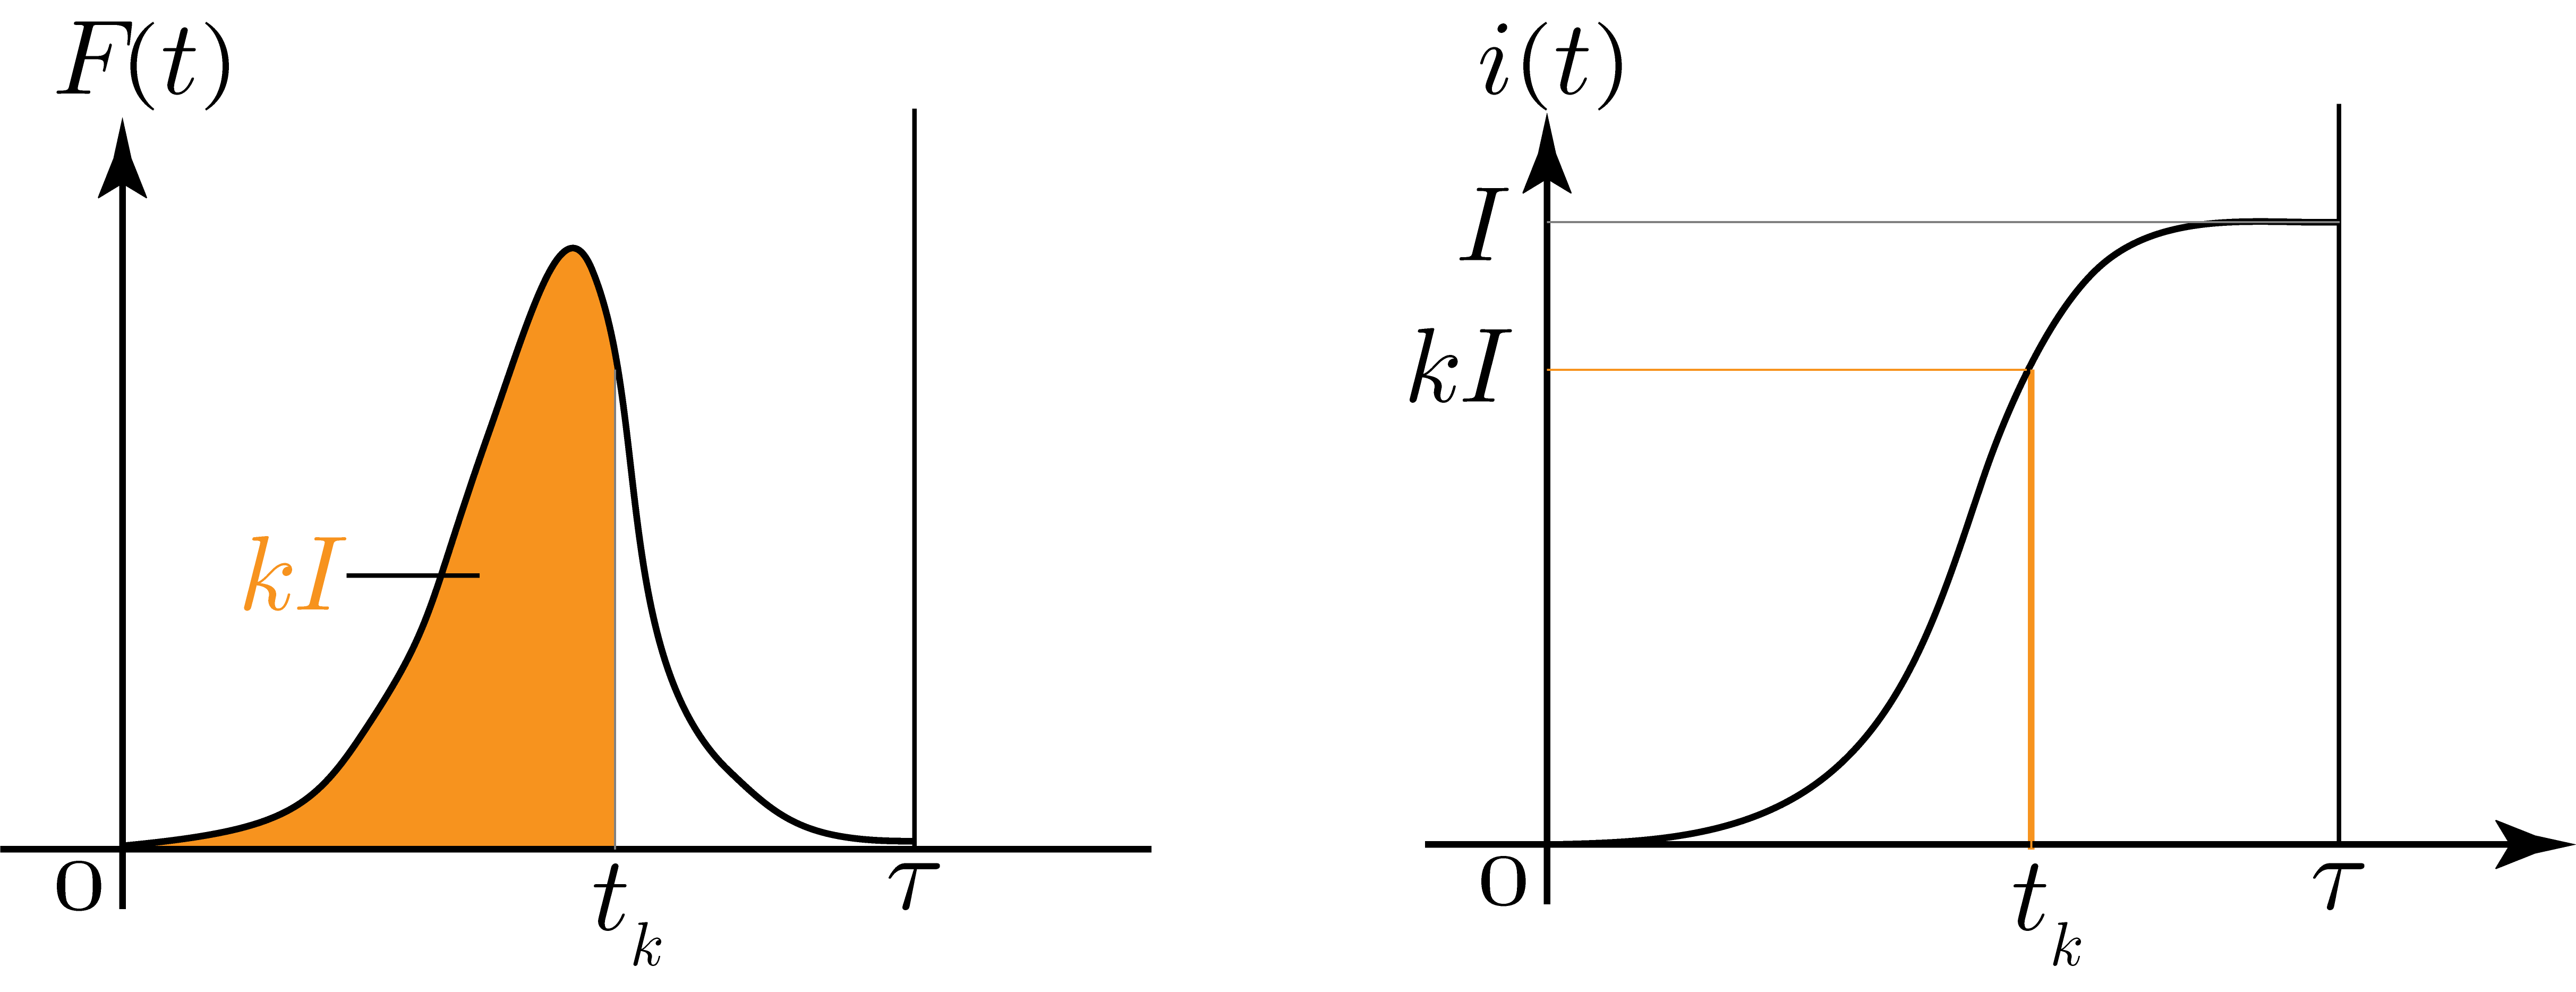
\includegraphics[width=16cm]{image/6-1-12.png}
\caption{力与累积的冲量}
\end{figure}


虽然这个问题倒是也分析地清,\,但这足以告诉我们,\,选取一个简单清晰的模型的必要性.\,为此我们进一步设出碰撞过程中两质点之间持续作用的力$F(t)$,\,它从$0$时刻开始产生到$\tau$时刻作用结束.\,但是,\,并不是只有两质点直接接触才发生作用力,\,事实上我们可以人为把这两个力加在相距较远的两个质点上,\,用这样的模型去等效本来可能复杂的碰撞过程.

我们再把过程中累积的冲量定义为一个函数:
\[i(t)=\int_0^t F(t')\ud t'\]

并且把最终造成的总作用冲量记作$I$:
\[I=\int_0^\tau F(t')\ud t'\]

那就必然有一个时刻冲量累积到$kI$,\,可以把这个时刻记作$t_k$,\,即:
\[i(t_k)=kI\]

事实上由于$i$是严格单调的增函数,\,就存在反函数$i^{-1}$,\,那么这个时间就是:
\[t_k=i^{-1}(kI)\]

有$i^{-1}(0)=0,\,i^{-1}(I)=\tau$.\,这样就足够我们去计算过程中相互作用力的做功了.\,由于是真实碰撞的模拟,\,那么必然$v_1\geq v_2$碰撞才可以发生.\,当冲量累积到$i$时,\,两个质点的速度分别为:
\[u_1=v_1-\frac{i}{m_1}\]
\[u_2=v_2+\frac{i}{m_2}\]

这说明过程$1$速度不断减小,\,$2$速度不断增加.\,现在就足够写出力对$1$和$2$做功的功率了.\,分别为:
\[P_1=-Fu_1=-\frac{\ud i}{\ud t}\left(v_1-\frac{i
}{m_1}\right)\]
\[P_2=Fu_2=\frac{\ud i}{\ud t}\left(v_2+\frac{i
}{m_2}\right)\]

最后如果把功率对时间积分,\,我们发现积分自动以$i$为自变量了:
\[W_1=\int_0^\tau P_1(t)\ud t=-\int_0^I \left(v_1-\frac{i
}{m_1}\right)\ud i\]
\[W_2=\int_0^\tau P_2(t)\ud t=\int_0^I \left(v_2+\frac{i
}{m_2}\right)\ud i\]

线性函数的积分,\,就等于函数值初末值的平均值乘以积分区间的长度,\,这就给出了一个\emph{冲量乘速度形式的功},\,碰撞过程中相互作用力对质点1和质点2的功应当是:
\[W_1=-\frac{1}{2}I(v_1+v_1')\]
\[W_2=\frac{1}{2}I(v_2+v_2')\]

这并不是任何让人意外的结论,\,如果带入动量定理$I=m_1(v_1-v_1')=m_2(v_2'-v_2)$就能发现这两个功无非就是末动能减初动能,\,其实就是反映了动能定律.\,不过注意到表达式推导过程中对动量定律的应用我们发现这个表达式倒不是纯粹的任意情况下都通用的功的定义.\,在使用动量定律前的这个功的积分:
\[W=\int \bs{v}\cdot \ud \bs{I}\]

倒是的确通用的.

如果定义碰前接触速度$v=v_1-v_2$,\,碰后分离速度$v'=v_2'-v_1'$.\,我们可以发现:
\[W_1+W_2=\frac{1}{2}I(v'-v)\]

又定义恢复系数$e=v'/v$.\,碰撞就因此分为四类:

1.\,完全非弹性碰撞,\,$I$最小的情况,\,作为一个实际的碰撞过程分离速度必然也至少为零$v_2'\geq v_1'$,\,否则1仍然在接近2力就不可能会消失.\,所以$I$最小就是让碰撞后共速,\,这样$e=0$就是完全非弹性碰撞的决定$I$大小的条件.

2.\,完全弹性碰撞.\,考虑碰撞过程的能量转化,\,显然,\,如果$W_1+W_2$不等于零,\,前后的总动能就不会是不变量.\,但是如果要求碰前碰后动能不变,\,这就构成了完全弹性碰撞,\,简称弹性碰撞.\,此时,\,除了可以列动能不变来求解$I$,\,我们发现这等价于$v=v'$,\,也就是\emph{接触速度等于分离速度}.\,以后我们将总是认为弹性碰撞的等价对应条件是$e=1$.

3.\,非弹性碰撞(不完全的).\,这是最符合实际情况的一类碰撞.\,这种碰撞中$0<e<1$.\,也就是$v'<v$的情况.\,功$W_1+W_2$是小于零的,\,说明碰撞过程动能有损失,\,能量去向是显而易见的:\,变成了两个碰撞的物体的内能,\,这里的内能可能就是热学上的内能,\,也可以是视作弹性体时虽然整体动量为零但局部有弹性波而产生的宏观动能与势能.\,这种情况之所以普遍是因为,\,碰前往往整个物体没有这样的弹性波,\,能量处于最低的状态,\,碰后这个能量总是会大于零.\,故能量总是有损失的.

4.\,超弹性碰撞.\,也就是$e>1$.\,碰撞后分离速度大于接触速度.\,因碰撞而获得动能.\,这样的过程也并不少见,\,炸弹的爆炸,\,或者刚刚的人推墙使人动起来都是这种情形.\,特点是别的能量会释放出来转化为动能.\,前提需要注意不能违背动量守恒.





\subsection{自由刚体的碰撞}

如果把两个质点的碰撞换为两个自由刚体相碰撞,\,这里我们只考虑平面情况,\,那么同理碰撞会产生一个冲量$\bs{I}$.\,但是这个冲量却有两种可能性,\,如果是光滑的刚体,\,那么碰撞的冲量必然沿法线$n$方向.\,但是如果是粗糙的刚体,\,那么还可以有沿切线方向的分量.\,不管何种情况我们来证明两个恒成立的结论:
\begin{wrapfigure}[14]{o}[-10pt]{6cm}\label{6-1-12}
\centering
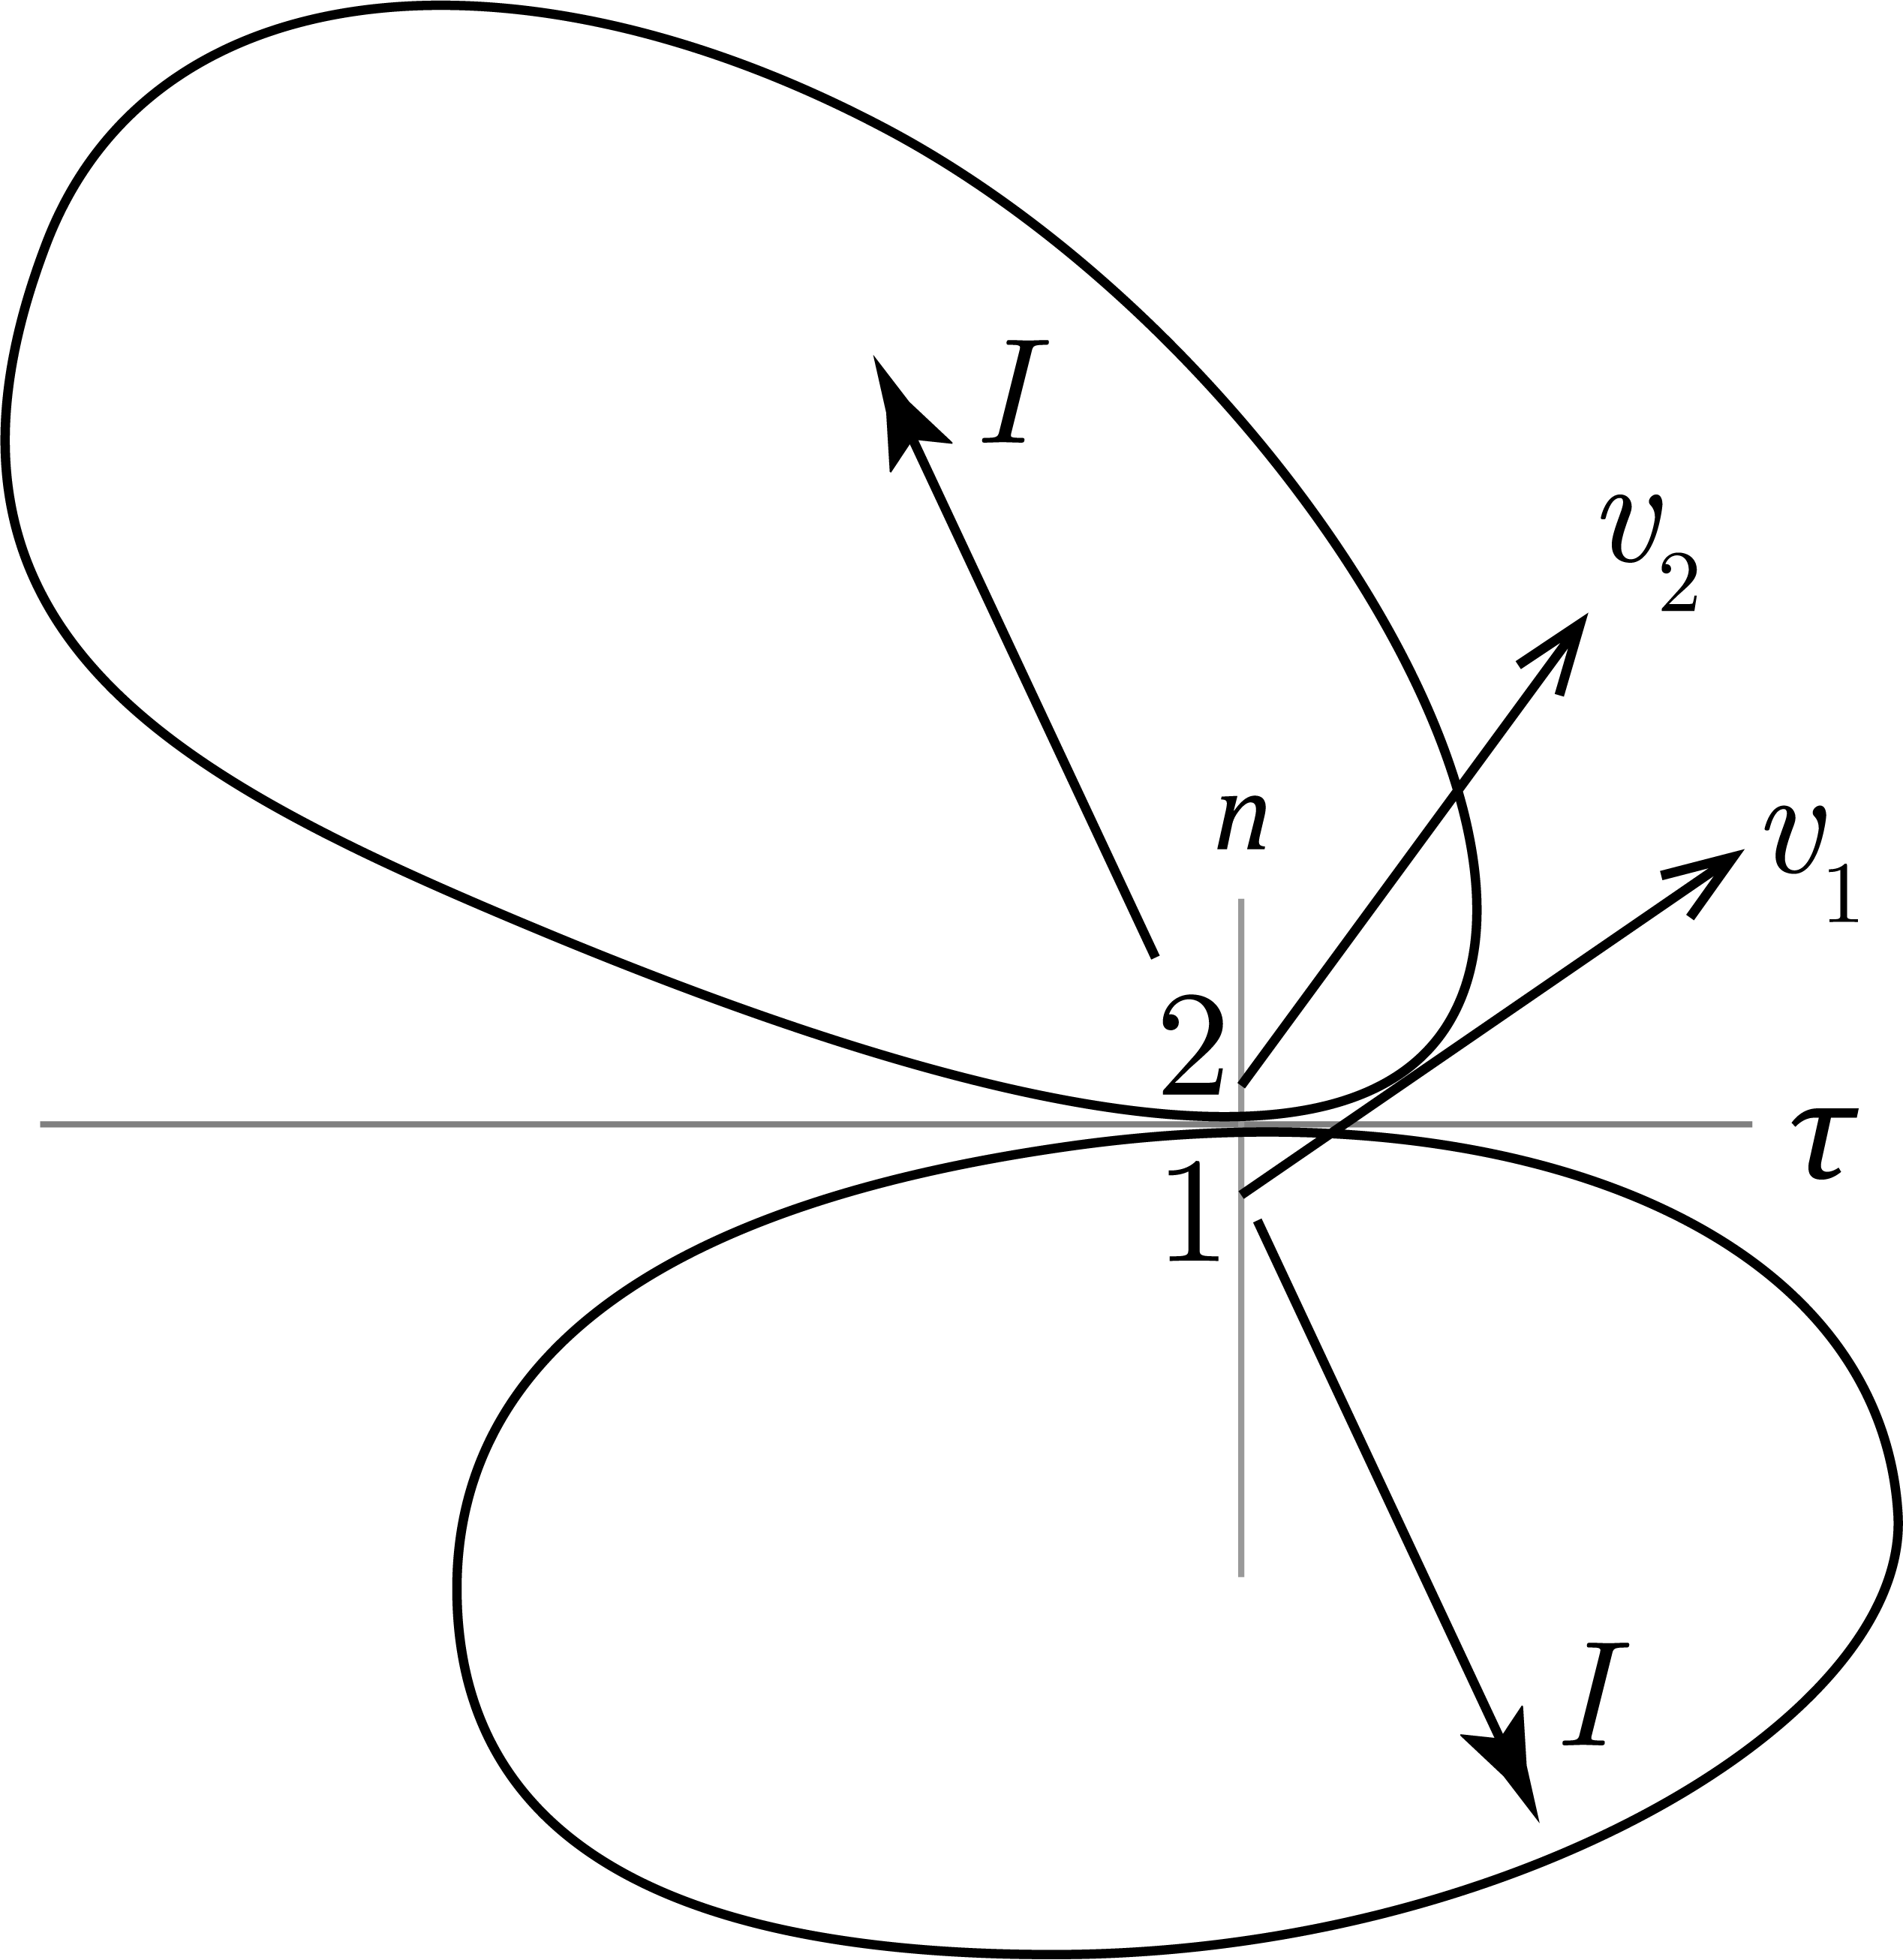
\includegraphics[width=6cm]{image/6-1-13.png}
\caption{两刚体碰撞}
\end{wrapfigure}

一是,\,1对2做的功或2对1做的功总是满足:
\[W=\frac{1}{2}\bs{I}\cdot(\bs{v}+\bs{v}')\]

这里$\bs{v}$和$\bs{v}'$指的便是力的作用点,\,即固连在刚体上的点的速度.\,证明这个定理思路类似于之前的做法.\,我们可以为过程中的冲量累计选取一个变量$k(t)$.\,当$k=0$时碰撞刚刚开始,\,而$k=1$时碰撞就结束了.\,变量取$k$时作用的冲量为:
\[\bs{i}(t)=k(t)\bs{I}\]

那么由于冲量对刚体质心速度和刚体旋转角速度的影响都是线性的,\,而且碰撞点速度也将线性依赖于这些值.\,从而积累到变量$k$时,\,点具有速度:
\[\bs{u}=k\bs{v}'+(1-k)\bs{v}\]

于是利用做功的积分式:
\[W=\int_0^\tau \bs{F}\cdot \bs{u}\ud t=\int_0^{\bs{I}} \bs{u}\cdot \ud \bs{i}=\int_0^1[k\bs{v}'+(1-k)\bs{v}]\cdot\bs{I}\ud k=\frac{1}{2}\bs{I}\cdot(\bs{v}+\bs{v}')\]

二是,\,不损失机械能的条件是,\,或者更特殊地,\,在无摩擦的碰撞中弹性碰撞的条件是,\,接触点形成的沿冲量方向的接触分速度等于该方向的分离分速度.\,这个证明也是简单的.\,只需要把点乘式后面的速度分解在冲量方向并把两个功相加为零即可.\,也就是我们有广义的$e=1$与动能不变作为弹性碰撞的等价条件.


\subsection{多体碰撞}
如果碰撞是多体的往往有两种不同的处理思路:\,一是屡次碰撞的思路,\,最典型的碰撞就是牛顿摆情况,\,小球与多个连续放置的小球的碰撞如果视作屡次的弹性碰撞就能解释体系形成周期性运动的原因.\,因为两个质量相等的小球的碰撞总是简单的交换速度.\,此时我们注意到碰撞结束后,\,最左侧的两球之间从接触速度的$v$变成了$0$,\,而最右侧的两小球却从$0$变成了$v$:
\begin{figure}[H]
\centering
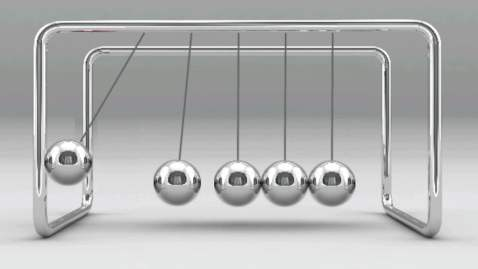
\includegraphics[width=16cm]{image/6-1-14}
\caption{牛顿摆}
\end{figure}

但是如果把最右边的小球要撞击的四个小球视作一个带约束的整体,\,显然既然四个小球必须作为一个整体运动,\,它们之间的相互作用冲量是不会做功的.\,同样的道理也适用于任何带约束的多体碰撞场合,\,虽然碰撞涉及多个物体,\,但是真正具有接触速度的只有一个碰撞点,\,那么作为约束其它点处不可能产生分离速度.\,从而动能不损失的条件依然是在撞击的点处法向接触速度等于分离速度.

不难理解,\,实际的多体碰撞总是介于两种极端情形之间的.\,如果是无限多个无限小的球无限密排,\,这就变成了一个连续的弹性介质中的波动的解的问题,\,波的传播速度和碰撞速度之间的大小关系就成为了一个具有决定性意义的因素.\,容易分析,\,思路一适用与撞击速度很快四个小球还来不及达到平衡的情况.\,而思路二适用于波的传播速度非常快,\,任何冲量作用在四个小球上都相当于在推动四个球构成的整体的情况.
%%!TEX root = ../physical-olympics-2.tex
\chapter{静力学}

以运动学和动力学理论为基础,\,时不时地,\,我们发现一些典型的现象,\,包括:
\begin{itemize}
	\item 不管体系多么复杂,\,能量函数对其行为似乎起决定性的作用.
	\item 似乎总是能够从不同的体系中抽象出它的一个特征数字:\,自由度.
	\item 约束越多体系约复杂,\,它的未知约束力越来越多,\,但是多到一定程度体系只剩下一个自由度了反而用能量守恒就能够解答大多数问题.
\end{itemize}

这些现象无疑是紧密联系的,\,值得研究的.\,事实上我们要做的就是以之前的所有动力学定律为依据进一步展开讨论.\,再从头开始建立新的理论:\,先讨论运动的描述,\,再单独研究力的特性.\,最后合到一起,\,看看这能让我们得到什么.

\section{约束}

\section{力系化简}

\section{平衡问题}

\section{虚功原理}

\section{分析力学初步}

\section{平衡态稳定性}

%%!TEX root = ../physical-olympics-2.tex
\chapter{简谐振动}


\section{方程与谐振}

\subsection{简谐振动的定义}
振动是最常见的物理现象.\,而振动中的最简单(simple)而和谐(harmonic)者谓之\emph{简谐振动}(simple harmonic oscillation).\,对\emph{谐振子}(harmonic oscillator)的学习与研究是会贯彻整个物理理论不同层次内容的始终的.\,现在是经典力学,\,以后会上升到场论,\, 量子力学与量子场论的高度.

简谐振动是指一个物理量$Q$随时间围绕其平衡位置做上下的波动.\,其形式符合:
\[Q=Q_0+\Delta Q\cos(\omega t+\varphi)\]

我们经常会有用复数表示振动的习惯,\,其做法是在三角函数$\cos$与其\emph{宗量}(argument)\,$\phi=\omega t+\varphi$构成的项后添加一个虚的$\ui \sin\phi$项,\,于是新的写法变成:
\[\tilde{Q}(t)=Q_0+\Delta Q\ue^{\ui(\omega t+\varphi)}\; ; \; Q=\mathfrak{Re}(\tilde{Q})\]

又或者:
\[\tilde{Q}(t)=Q_0+\Delta \tilde{Q}\ue^{\ui\omega t}\; ; \; \Delta \tilde{Q}=\Delta Q\ue^{\ui\varphi}\]

以上各个常量中,\,$Q_0$是平衡位置,\,$\Delta Q$叫\emph{振幅}(amplitude),\,宗量$\omega t+\varphi$叫做\emph{相位}(phase),\,$\omega$叫\emph{角频率}(angular frequency),\,$\varphi$叫初相位.\,$\tilde{Q}$为复化的复物理量,\,而$\Delta \tilde{Q}$叫做\emph{复振幅}(complex amplitude).

复数表示最大的一个好处就在于很方便计算物理量的线性组合与导数.\,事实上,\,如果合理选取$Q_0=0$:
\[\dot{Q}=-\omega\Delta Q\sin\phi\; ; \; \dot{\tilde{Q}}=\ui\omega\tilde{Q}\quad \Rightarrow\quad \dot{Q}=\mathfrak{Re}(\dot{\tilde{Q}})\]
\[\ddot{Q}=-\omega^2\Delta Q\cos\phi\; ; \; \ddot{\tilde{Q}}=-\omega^2\tilde{Q}\quad \Rightarrow\quad \ddot{Q}=\mathfrak{Re}(\ddot{\tilde{Q}})\]

\subsection{简谐振动的性质}
以一个质点水平坐标$x$围绕$x=0$左右做谐振为例.\,其运动方程写作\footnote{以后我们对物理量和物理量的复化只在必要的时候加以区分,\,看到复数只需要认为省写了取实部这一例常操作罢了.}:
\[x=A\ue^{\ui(\omega t+\varphi)}\]

那么其速度与加速度为:
\[v=\ui\omega A\ue^{\ui(\omega t+\varphi)},\,a=-\omega^2A\ue^{\ui(\omega t+\varphi)}\]

我们发现在运动过程中的任意一个时刻,\,加速度都是指向平衡位置的,\,与偏离平衡位置的位移是成正比的:
\[a=-\omega^2 x\]

而任意一个时刻既然$x$是宗量的余弦函数,\,$v$是正弦函数,\,它们就满足其绝对值大小的``此消彼长''关系\footnote{注意到这里(往下)要避免使用复数,\,因为一个复数的实部平方不会等于其平方的实部$v^2\neq\mathfrak{Re}(\tilde{v}^2)$}:
\[v^2+\omega^2 x^2=\omega^2 A^2\]

相位是很重要的物理概念,\,\emph{相}(phase),\,状态也,\,相位则是一个可以用来表示状态的数.\,反过来,\,我们可以根据物体在一个时刻的状态反过来确定这个时刻的相位.\,如果位移是$x$而振幅为$A$,\,则:
\[\phi=\mathrm{Arcsin}\frac{x}{A}\, ,\,\mathrm{Arcsin}\frac{x}{A}\in \left\{\arcsin\frac{x}{A}+2n\pi|n\in\mathbb{Z}\right\}\cup\left\{\pi-\arcsin\frac{x}{A}+2n\pi|n\in\mathbb{Z}\right\}\]

同理如果已知速度$v$和\emph{速度振幅}(velocity amplitude)\,$\omega A$,\,那么相位为:
\[\phi=\mathrm{Arccos}\frac{v}{\omega A}\, ,\,\mathrm{Arccos}\frac{v}{\omega A}\in \left\{\arccos\frac{v}{\omega A}+2n\pi|n\in\mathbb{Z}\right\}\cup\left\{-\arccos\frac{v}{\omega A}+2n\pi|n\in\mathbb{Z}\right\}\]

相位的取法上具有多值性.\,但是相位随时间的变化我们约定必须是连续的,\,事实上它随时间线性增加.\,也就是说如果前一个状态下相位为$\phi_1$,\,后一个状态下相位为$\phi_2$,\,那么这两个状态间历时:
\[\Delta t=\frac{\phi_2-\phi_1}{\omega}\]

\subsection{简谐振动的判定}

事实上以上的两个关系都可以成为体系做简谐振动的判据,\,它们为:

\begin{itemize}
	\item 线性回复判据:\,如果一个随时间演化的变量的二阶导数正比于变量本身,\,且符号相反,\,可以判断变量做简谐振动:
	\[\ddot{q}=-\omega^2 q\quad \Rightarrow \quad q=A\cos(\omega t+\varphi)\]

	\item 此消彼长判据:\,如果一个随时间演化的变量的一阶导数与自己的正系数平方和为动力学守恒量(一般就是能量).\,可以判断变量做简谐振动:
	\[\dot{q}^2+\omega^2 q^2=\omega^2A^2\quad \Rightarrow \quad q=A\cos(\omega t+\varphi)\]
\end{itemize}

证明如下:

线性回复$\Rightarrow$此消彼长:

首先进行代换:

\[\ddot{q}=\frac{\ud}{\ud t}(\dot{q})=\frac{\ud q}{\ud t}\frac{\ud}{\ud q}(\dot{q})=\frac{\dot{q}\ud\dot{q}}{\ud q}\]

将上式代入$\ddot{q}=-\omega^2 q$:
\[\dot{q}\ud\dot{q}+\omega^2 \cdot q\ud q=\ud(\frac{1}{2}\dot{q}^2+\frac{1}{2}\omega^2 q^2)=0\quad \Rightarrow \quad \dot{q}^2+\omega^2 q^2=C\]

命$A=\sqrt{C/\omega^2}$即得到此消彼长判据.

此消彼长$\Rightarrow$简谐振动:

考虑$\dot{q}$的正根即可,\,负根结果也是简谐振动:
\[\dot{q}=\frac{\ud q}{\ud t}=\omega\sqrt{A^2-q^2}\]
\[\Rightarrow \quad \frac{\ud q}{\sqrt{A^2-q^2}}=\omega \ud t\]

两边同时积分,\,积分常数写到右侧记作$\varphi$,\,得到:
\[-\arccos \frac{q}{A}=\omega t+\varphi \quad \Rightarrow\quad q=A\cos(\omega t+\varphi)\]
\vspace{-0.1cm}


\subsection{小振动}

值得注意的是,\,很多情况下体系的运动并不是严格的简谐振动.\,十分常见的一种情况是\emph{小振动}(small oscillation).\,事实上,\,如果我们研究体系为完整而稳定的一自由度体系,\,广义坐标为$q$,\,而且势能函数$V(q)$存在一个极小值:
\[V'(q_0)=0\quad,\quad V''(q_0)>0\]

那么根据上一章的阐述,\,这个$q_0$就是体系的稳定平衡位置.\,那么,\,任何偏离这个平衡位置的系统运动只要偏离的值足够小,\,即做坐标变换$\delta=q-q_0$为无穷小量,\,那么就一定为简谐振动.\,这是因为势能可以由泰勒展开为:
\[V=\frac{1}{2}V''(q_0)\delta^2+\frac{1}{3!}V'''(q_0)\delta^3+\cdots\]

只要$\delta$足够小,\,三阶项就必然远小于二阶项.\,从而可以只保留第一项.\,同理这也适用于动能,\,它必然正比于$\dot{\delta}$的平方,\,系数则与平衡位置有关:
\[T=\frac{1}{2}M(q_0)\dot{\delta}^2\]

从而这个体系的能量函数(哈密顿量)就被近似为了:
\[H=T+V=\frac{1}{2}M(q_0)\dot{\delta}^2+\frac{1}{2}V''(q_0)\delta^2\]

这就直接符合了``此消彼长''判据.\,从而小振动的角频率为:
\[\omega=\sqrt{\frac{V''(q_0)}{M(q_0)}}\]

例如,\,在典型的单摆问题中,\,取摆线与竖直方向的夹角$\theta$为广义坐标.\,摆球的重力势能以平衡位置为原点表示为:
\[V(\theta)=mgl(1-\cos\theta)\]

而动能为:
\[T=\frac{1}{2}ml^2\dot{\theta}^2\quad \Rightarrow\quad M(\theta)=ml^2\]

从而只需要带入以上公式,\,就得到:
\[\omega=\sqrt{\frac{V''(0)}{M(0)}}=\sqrt{\frac{mgl}{ml^2}}=\sqrt{\frac{g}{l}}\]

这是因为事先看出来了稳定平衡点为$\theta=0$.\,简单的小振动问题的思路都大抵如此.\,第一步是写出能量函数来,\,它决定体系的所有可能的动力学演化.\,第二步要找到稳定平衡位置,\,往往一样地是通过势能函数的增减凹凸性来判断,\,往往也要结合体系的对称性来观察.\,最后便是在平衡位置处把动能势能都近似为简单的平方项.\,唯一需要补充的是,\,除了利用二阶导数来计算这一个平方项,\,对常见函数写泰勒展开式也是十分常见的思路.

单摆问题的周期从而就是:
\[T=\frac{2\pi}{\omega}=2\pi\sqrt{\frac{l}{g}}\]

但是一定要注意这个振动仅仅对小振动成立.\,例如在摆角为$10\dgr=0.087{\rm rad}$时会有约$2\permil$的误差.\,如何计算这个误差?\,之后的非线性振动将讨论这个问题.


\section{阻尼振动与受迫振动}

\subsection{阻尼振动}

阻尼振动,\,狭义地是指普通的弹簧型谐振子,\,但是让振子运动的空间充满介质而产生湿摩擦(流体摩擦).\,从而产生一个正比于速度的阻尼的情形.\,其牛顿定律为:
\[m\ddot{x}=-kx-\gamma \dot{x}\]

这里的$\gamma$即\emph{阻尼系数}(damping coefficient).\,习惯上把$m/\gamma$称作\emph{弛豫时间}(relaxation time).\,最后还定义\emph{衰减参数}(attenuation parameter)或\emph{损耗参数}(loss parameter)为:
\[\beta=\frac{\gamma}{2m}\]

而无阻尼情况下的\emph{固有频率}(natural frequency), 这里是角频率,\,为:
\[\omega_0=\sqrt{\frac{k}{m}}\]

这样原来的方程又被重新写为:
\[\ddot{x}+2\beta \dot{x}+\omega_0^2 x=0\]

我们定义广义的\emph{阻尼振动}(damped oscillation),\,只需要一个运动的任意自由度$q$,\,符合或者可以近似为以上式子形式的动力学方程,\,那么这个自由度上的运动就是一个阻尼振动.\,所有的阻尼振动只有两个常数特征,\,一个是固有角频率,\,一个是损耗的大小.

\vspace{1cm}
阻尼振动的求解需要分为三种情况.\,我们统一猜解:
\[x=A\ue^{\ui\omega t}\]

带入原方程以后发现$\omega$需要满足:
\[\omega^2-2\ui\beta\omega-\omega_0^2=0\]

从而:

\begin{itemize}
	\item \emph{欠阻尼}(underdamped)

	常见的小阻尼情况,\,此时$0<\beta<\omega_0$.\,通过对以上方程求解得到两个含有正虚部的关于虚轴对称的根:
	\[\omega_{1,2}=\ui\beta \pm\sqrt{\omega_0^2-\beta^2}\]

	这样就得到了原阻尼振动方程的通解:
	\[x=\ue^{-\beta t}[A\cos(\sqrt{\omega_0^2-\beta^2}t)+B\sin(\sqrt{\omega_0^2-\beta^2}t)]=C\ue^{-\beta t}\cos(\sqrt{\omega_0^2-\beta^2}t+\varphi)\]

	\begin{figure}[H]
	\centering
	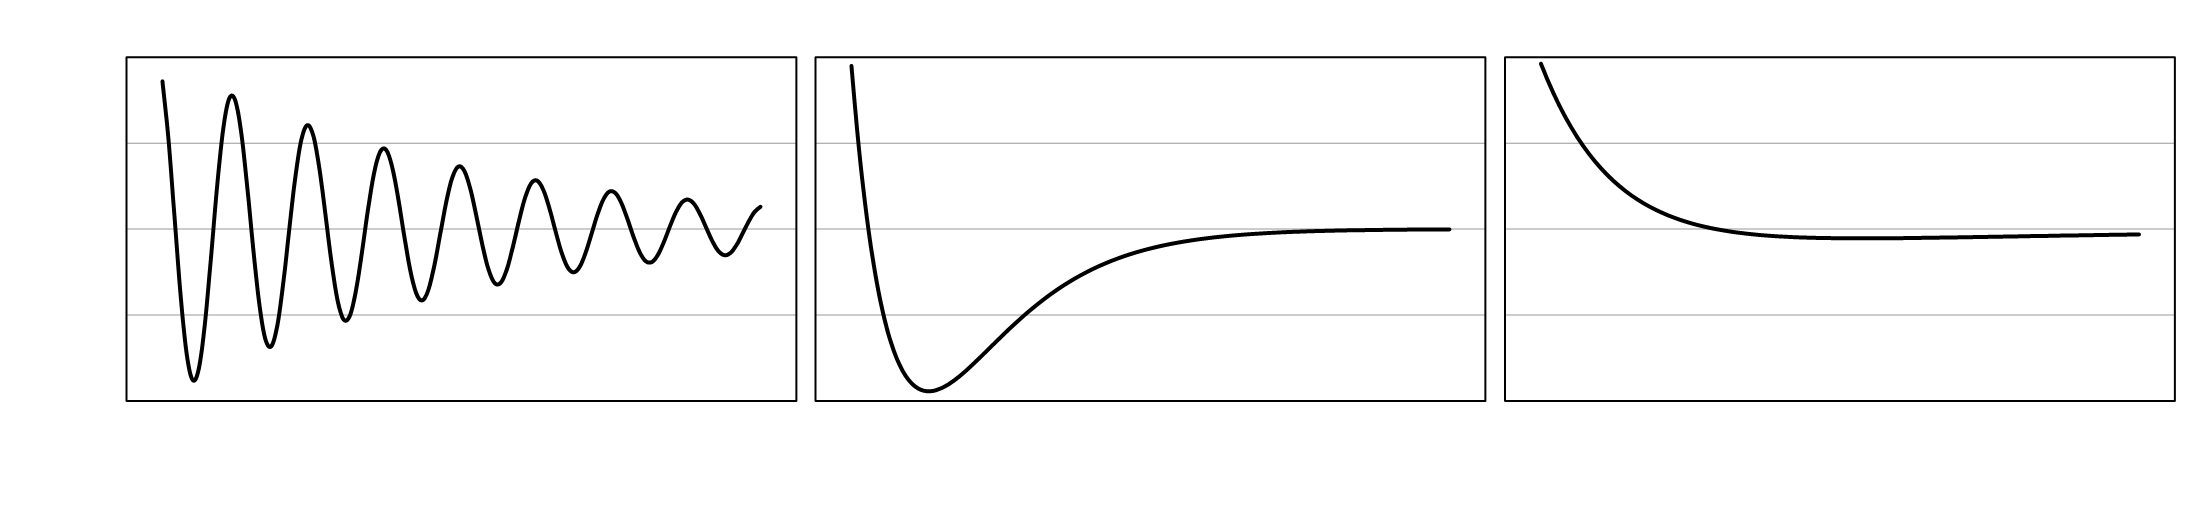
\includegraphics[width=14cm]{image/6-3-1.png}
	\caption{欠阻尼, 临界阻尼与过阻尼}
	\end{figure}

	\item \emph{过阻尼}(overdamped)

	此时$\beta>\omega_0$.\,从而振动和回复力被极大地抑制了.\,主要是一个在大阻力和初速度下缓慢回到平衡位置的运动.\,以上方程两根此时为两个正虚根:
	\[\omega_{1,2}=\ui(\beta\pm\sqrt{\beta^2-\omega_0^2})\]

	这样就得到了原阻尼振动方程的通解:
	\[x=\ue^{-\beta t}[A\ue^{\sqrt{\beta^2-\omega_0^2}t}+B\ue^{-\sqrt{\beta^2-\omega_0^2}t}]=C\ue^{-\beta t}\cosh(\sqrt{\beta^2-\omega_0^2}t+\varphi)\footnote{也有可能是$\sinh$}\]

	\item \emph{临界阻尼}(critical damped)

	这对应$\beta=\omega_0$的特殊情况.\,可以通过微分方程的理论,\,或者采用求$\beta\to \omega_0$极限的方式得到此时的运动方程.\,它为:
	\[x=\ue^{-\beta t}(A+Bt)\]

	临界阻尼在实际生活中的应用为:\,它是较快能够让振子回到平衡位置的理想阻尼大小.\,这一点不难理解,\,不难看出,\,欠阻尼情况的振幅随时间的衰减方式为$\ue^{-\beta t}$,\,也就是适当增大$\beta$有利于振幅尽快衰减.\,但是,\,过阻尼时,\,长时间后位移与时间的关系为
	\[x\sim \ue^{-\beta t}\cosh(\sqrt{\beta^2-\omega_0^2}t)\sim\ue^{-\beta t}\ue^{\sqrt{\beta^2-\omega_0^2}t}\sim \ue^{-\frac{\omega_0^2t}{\beta+\sqrt{\beta^2-\omega^2}}}\]

	这就不难发现,\,此时增加$\beta$只会使得$t$前的衰减系数变小而不利于尽快衰减其位移.\,从而,\,无论是欠阻尼还是过阻尼,\,临界阻尼是它们能够尽快回到平衡位置的极限.\,此时原来的固有频率对应的周期就是它回到平衡位置的特征时间.
\end{itemize}

对于欠阻尼情况,\,尤其是衰减因子$\beta<<\omega_0$的小阻尼情况,\,还有一些重要的性质值得挖掘.\,下面都默认是这样的前提:

\begin{wrapfigure}[17]{o}[-10pt]{7cm}
\centering
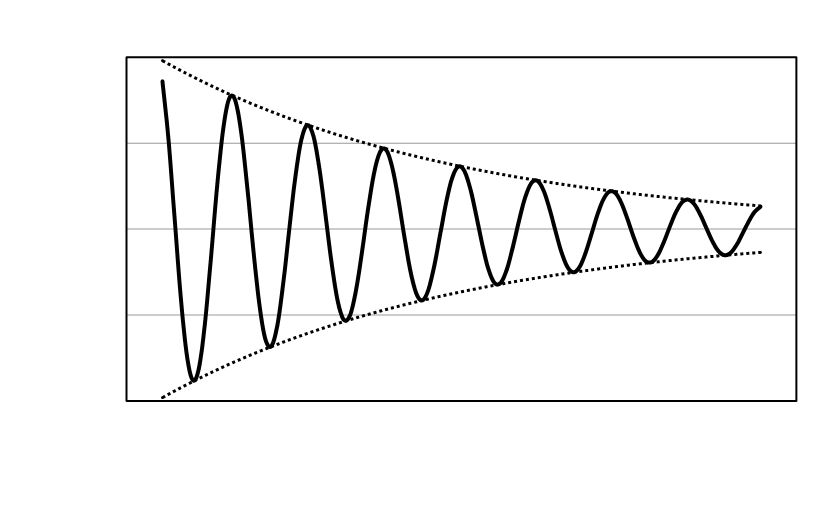
\includegraphics[width=7cm]{image/6-3-2.png}
\caption{\quad 小阻尼下的振幅衰减}
\end{wrapfigure}
从之前的运动方程解不难看出来,\,我们可以把小阻尼情况下的运动方程看作是一个振幅不断随着时间衰减的简谐振动.\,其振幅衰减函数和阻尼化角频率为:
\[A(t)=A_0\ue^{-\beta t}\]
\[\omega_d=\sqrt{\omega_0^2-\beta^2}\approx \omega_0\]

要讨论其衰减的原因,\,还有一种新的角度,\,便是考虑其能量.\,当振幅为$A$时,\,其动能,\,势能的和为:
\[E=T+V=\frac{1}{2}m\dot{x}^2+\frac{1}{2}kx^2\]

现在它不是守恒的,\,仅仅是在少数几个周期里面``近似''守恒.\,但是我们可以考虑求它在一个周期内的平均:
\[\bar{E}=\frac{1}{2}\cdot\frac{1}{2}m\omega_d^2 A^2+\frac{1}{2}\cdot\frac{1}{2} kA^2=\frac{1}{2}m\frac{\omega_0^2+\omega_d^2}{2} A^2\approx \frac{1}{2}m\omega_0^2 A^2\]

现在我们计算单位时间减少的能量的平均值.\,它其实就是阻尼造成的负功功率的平均值:
\[\bar{P}=\overline{\gamma v\cdot v}=\frac{1}{2}\gamma \omega_d^2 A^2\approx \frac{1}{2}\gamma \omega_0^2 A^2=\frac{1}{2}m \omega_0^2 A^2\cdot 2\beta\]

通过损耗功率等于能量的负导数,\,也可以得到振幅随着时间衰减的具体结果.\,我们现在关心一个重要的量,\,它实际上是反应振子振动单位时间所减少的能量占由于以$\omega_0$振动导致的总能量转化速率的比例,\,我们把上式换一种写法:
\[\bar{P}=\frac{\omega_0\bar{E}}{Q}\]

以上引入的$Q$就是著名的\emph{品质因数}(quality factor).\,它越大,\,表示损耗越低,\,振子的阻尼就越小,\,就越接近``谐振''.\,实际上它算法为:
\[Q=\frac{\omega_0}{2\beta}\]

品质因数经常与另一个因子一起提出,\,两者是简单的倒数关系,\,更精确地,\,我们定义:
\[\sin\delta=\frac{1}{2Q}=\frac{\beta}{\omega_0}\]

$\delta$被称作\emph{损耗角}(loss angle).\,一定要注意这两个概念是普遍的.\,谐振子模型是很多实际问题的抽象,\,它们作为谐振子都有自己的品质因数或损耗角,\,用以描述过程的一些共性,\,而且,\,不光可以用能量的损失的共性来定义品质因数和损耗角,\,还有很多重要的方式.\,详情见后.

\begin{wrapfigure}[17]{o}[-10pt]{7cm}
\centering
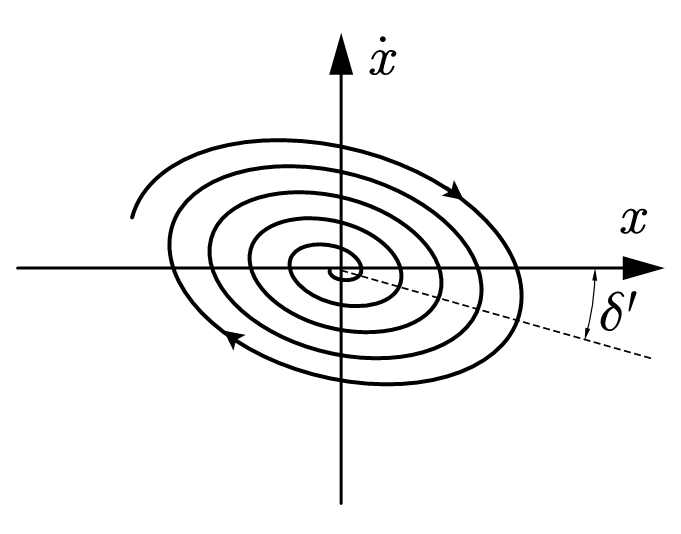
\includegraphics[width=7cm]{image/6-3-3.png}
\caption{阻尼振动的相图}
\end{wrapfigure}
现在我们来考虑简谐振动的\emph{相图}(phase diagram).\,在动力学中,\,这总是指把单个过程的运动,\,画成以其广义坐标和广义速度(或动量)为坐标轴的\emph{相空间}(phase space)中的曲线形成的图像.\,阻尼振动的代表性解为:
\[x=A\ue^{-\beta t}\ue^{\ui \omega_d t}\]

在这个解下,\,其速度为:
\[\dot{x}=(\ui\omega_d-\beta)A\ue^{-\beta t}\ue^{\ui \omega_d t}\]

两个量都在随时间衰减.\,从而在相图上就体现为一随着时间不断向着原点靠近的螺旋线.\,如果没有阻尼,\,那么标准简谐振动的相轨迹就是正椭圆:
\[\frac{x^2	}{A^2}+\frac{\dot{x}^2}{\omega_0^2A^2}=1\]

但是,\,有阻尼时除了是螺旋式的椭圆,\,它还不是``正''的.\,事实上,\,如果去除衰减因子,\,即将$x$和$\dot{x}$乘以个$\ue^{\beta t}$以抵消其衰减:
\[X=x\ue^{\beta t}=A\ue^{\ui \omega_d t}\quad,\quad V=\dot{x}\ue^{\beta t}=\ui(\omega_d+\ui\beta)A\ue^{\ui \omega_d t}\]

两者之间也不是恰好相差相位$\pi/2$,\,而是有一个额外相位差:
\[\delta=\arctan\frac{\beta}{\omega_d}=\arcsin\frac{\beta}{\omega_0}\]

可以发现这个相位差就是损耗角.\,也就是说,\,损耗角的另一种理解方式是位置与速度振动过程中的相位夹角.\,作为结果,\,其相图中的椭圆也要倾斜一个角度$\delta'$.\,可以证明,\,损耗角越大,\,这个倾斜角度也会越大.

\subsection{受迫振动}

如果在谐振子上施加一个周期性的策动外力.\,我们总是研究基本的简谐式的外力\footnote{傅里叶分析理论告诉我们,\,任何函数都可以分解为无穷多助三角函数的线性组合.\,故对于线性系统原则上就可以用叠加原理处理任意任意强迫力的运动求解:\,只要我们把简谐强迫力找到解法.}:
\[F(t)=F_0\ue^{\ui\omega t}\quad {\rm i.e.}\quad F(t)=F_0\cos{\omega t}\]

这个运动就称作\emph{受迫振动}(driven oscillation).\,这样子原来的方程就变为:
\[m\ddot{x}+\gamma\dot{x}+kx=F_0\ue^{\ui\omega t}\]
\[\Rightarrow\quad \ddot{x}+2\beta\dot{x}+\omega_0^2 x=\frac{F_0}{m}\ue^{\ui\omega t}\]

很明显,\,可以猜一个谐振解.\,它是上述微分方程的特解(稳态解).\,通解还需要加上上一部分讨论的阻尼振动解(齐次方程的解是暂态解).\,注意其振动频率应当是策动力的频率$\omega$而不是体系的固有频率$\omega_0$:
\[x=A\ue^{\ui\omega t}\quad \Rightarrow \quad (\omega_0^2-\omega^2+2\ui\beta\omega)A=\frac{F_0}{m}\]

故,\,复振幅的解法也是相当地直接:
\[A=\frac{F_0/m}{\omega_0^2-\omega^2+2\ui\beta\omega}\]


作为复振幅,\,上$A$表达式其实同时包含了两个因素,\,一个是振幅,\,一个是相位.\,现在我们分离它们:
\[A=|A|\ue^{\ui \varphi}\]
\[|A|=\frac{F_0/m}{\sqrt{(\omega_0^2-\omega^2)^2+4\beta^2\omega^2}}\]
\[\varphi=-\arctan\frac{2\beta\omega}{\omega_0^2-\omega^2}\quad {\rm or} \quad \varphi=-\left(\pi-\arctan\frac{2\beta\omega}{\omega^2-\omega_0^2}\right)\]

\begin{wrapfigure}[15]{o}[-10pt]{7cm}
\centering
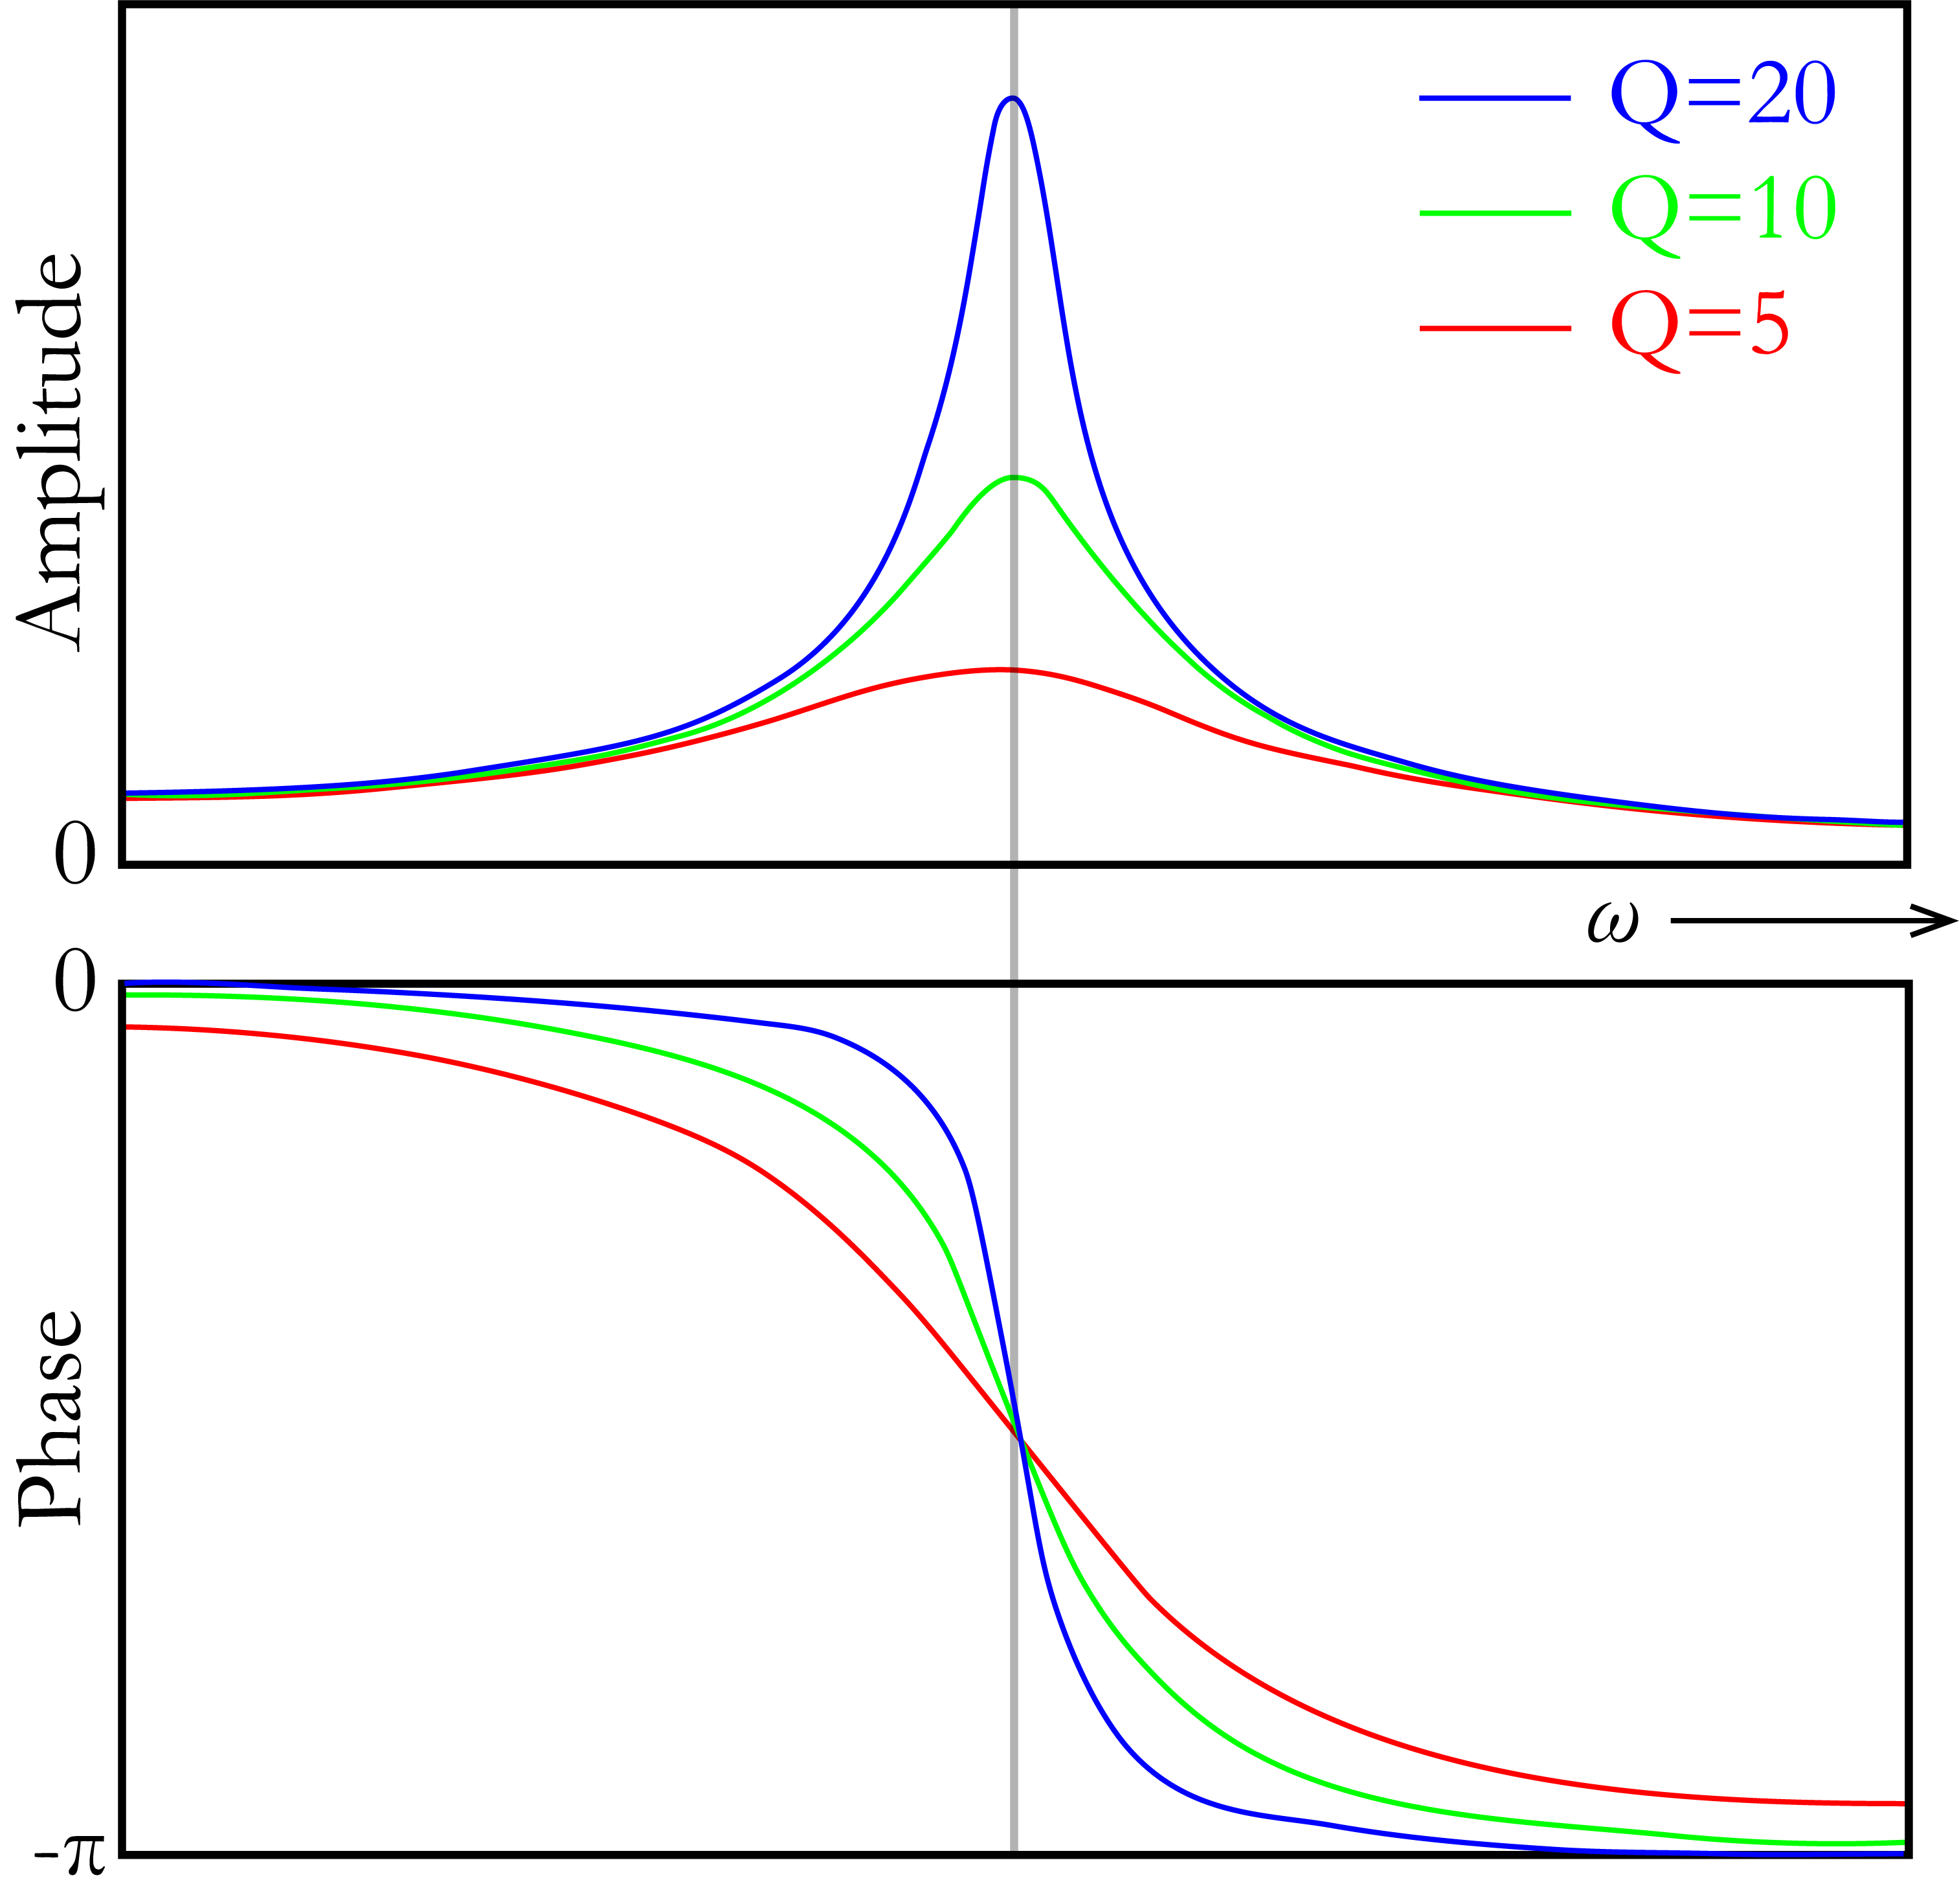
\includegraphics[width=7cm]{image/6-3-4.png}
\caption{幅频, 相频特性}\label{6-3-4}
\end{wrapfigure}
这就构成了两个关于$\omega$的函数.\,这也是实验上我们特别关心的两个函数,\,它们反映在稳态受迫振动的时候,\,一定外力下振子产生的振幅与相位究竟是怎样取决于策动力的角频率的.\,这就是著名的\emph{幅频特性}(amplitude-frequency characteristic)和\emph{相频特性}(phase-frequency characteristic).\,利用之前定义的品质因数$Q$,\,再命$x=\omega/\omega_0$.\,整理得:
\[|A|=\frac{QF_0/m\omega_0^2}{\sqrt{Q^2(1-x^2)^2+x^2}}\]
\[\varphi=-\arccos\frac{Q (1-x^2)}{\sqrt{Q^2(1-x^2)^2+x^2}}\]


我们依然只考虑小阻尼情况.\,此时$Q$较大.\,比如如图\ref{6-3-4}所示,\,$Q=5,\,10,\,20$等.

那么受迫振动又被分为三种情形:

\begin{itemize}
	\item 低频区为弹性控制区.

	在$\omega\ll\omega_0$时,\,$m\ddot{x},\,\gamma\dot{x},\,kx$三项中最后一项最大,\,主要是弹簧的弹性力与策动力去平衡.\,从而体现出以下计算结果:
	\[|A|\approx \frac{F_0}{m\omega_0^2}=\frac{F_0}{k}\]
	\[\varphi\approx 0\]

	也就是策动力与位移几乎同相,\,振子有充分的时间去实现平衡.

	\item 高频区为惯性控制区.

	在$\omega\ll\omega_0$时,\,$m\ddot{x},\,\gamma\dot{x},\,kx$三项中第一项最大,\,主要是高速变化的策动力去直接产生振子加速度.\,从而体现出以下计算结果:
	\[|A|\approx \frac{F_0}{mx^2\omega_0^2}=\frac{F_0}{m\omega^2}\]
	\[\varphi\approx -\pi\]

	也就是策动力与位移几乎反相(亦反向).\,振子``随波逐流'',\,弹性力和阻尼力没有时间跟上策动力的节奏.

	\item 中频区为共振区.

	在$\omega$在$\omega_0$附近,\,即量级接近时.\,三个项$m\ddot{x},\,\gamma\dot{x},\,kx$也量级相当.\,如果把结果画成图\ref{6-3-4}.\,可以发现十分典型的现象是,\,振幅在某频率处取到了极值.\,而相位差(绝对值)在某频率处从小于$\pi/2$增加到大于$\pi/2$.
\end{itemize}

\emph{共振}(resonance)是谐振子系统中十分典型的现象.\,一个共振发生的时候有两个量是值得关注的:

第一个值得关注的共振参数,\,是共振的峰的位置.\,即\emph{共振频率}(resonance frequency).\,但是这个因素又被分为位移共振和速度共振,\,即位移振幅$|A|$最大或者速度振幅最大的角频率值.\,或者可以证明,\,等价的是,\,\emph{振幅共振}(amplitude resonance)和\emph{相位共振}(phase resonance).\,前者指的是响应$x$最大的点:
\[x^2=1-\frac{1}{2Q^2}\approx 1\quad \Rightarrow \quad \omega\approx\omega_0\]

后者则指响应和策动力完全相位差为$\pi/2$的情况:
\[x^2=1\quad \Rightarrow \quad \omega=\omega_0\]

可见两个共振在小阻尼情况下几乎是重合的.\,在振幅共振的情况下,\,振幅最终为:
\[|A|=Q\cdot\frac{F_0}{m\omega_0^2}\cdot\sqrt{\frac{4Q^2}{4Q^2-1}}\approx Q\cdot\frac{F_0}{m\omega_0^2}\]

如果以这个角频率的外力$F_0$直接作用在自由的质点上,\,或者是考虑让一个没有阻尼的振子进行固有振动并使弹簧给振子的力就是$F_0$.\,我们发现振子振幅应当是$F_0/m\omega_0^2$.\,这就是说共振时振幅成为了这个振幅的$Q$倍.\,说明了如果让体系从静止开始,\,自某一时刻开始受到周期性的外力而产生振动,\,如果频率接近固有频率,\,体系会十分反常的振幅越来越大,\,直到振幅是自由振幅的$Q$倍.\,这也是品质因数的第二种理解方式:\,共振的放大倍数.

在看相位共振时的策动力-相位差为$\pi/2$的现象.\,这说明了什么?\,这说明策动力与速度完全就是同相的.\,带入$x=1$容易计算此时位移振幅为$|A|=QF_0/m\omega_0^2$,\,等效地可以写成$F_0=m\omega_0^2|A|/Q$.\,那么速度振幅就是$\omega_0|A|$.\,从而策动力对速度单位时间做的功就是:
\[W=\overline{F(t)\dot{x}(t)}=\frac{1}{2}F_0\omega_0|A|=\left.\frac{1}{2}m\omega_0^3|A|^2\right/ Q\]

这与上一部分得到了相似的结果.\,因为振动的能量其实就是:
\[\bar{E}=\frac{1}{2}m\omega_0^2|A|^2\]

也就是说品质因数反映了耗散的能量与总能量(动能势能互相转换)的比例:
\[Q=\frac{\omega_0 \bar{E}}{W}\]

第二个值得关注的共振参数,\,是共振的峰的宽度.\,谐振子模型给出的幅频曲线,\,与著名的\emph{柯西分布}(Cauchy distribution)对应的函数曲线有密切联系,\,柯西分布又常常因为在理论物理学中的广泛使用而称作\emph{洛伦兹型}(lorentzian shape)\footnote{比如谱线的形状,\,即线型,\,就常被视作洛伦兹线型.}.\,所谓柯西分布最初来自概率分布模型,\,它是指以下分布函数:
\[{\rm pdf.}\footnote{probability distribution function,\,即概率分布函数的缩写.}=\frac{1}{\pi[\gamma^2+(x-x_0)^2]}\]

\begin{figure}[H]
\centering
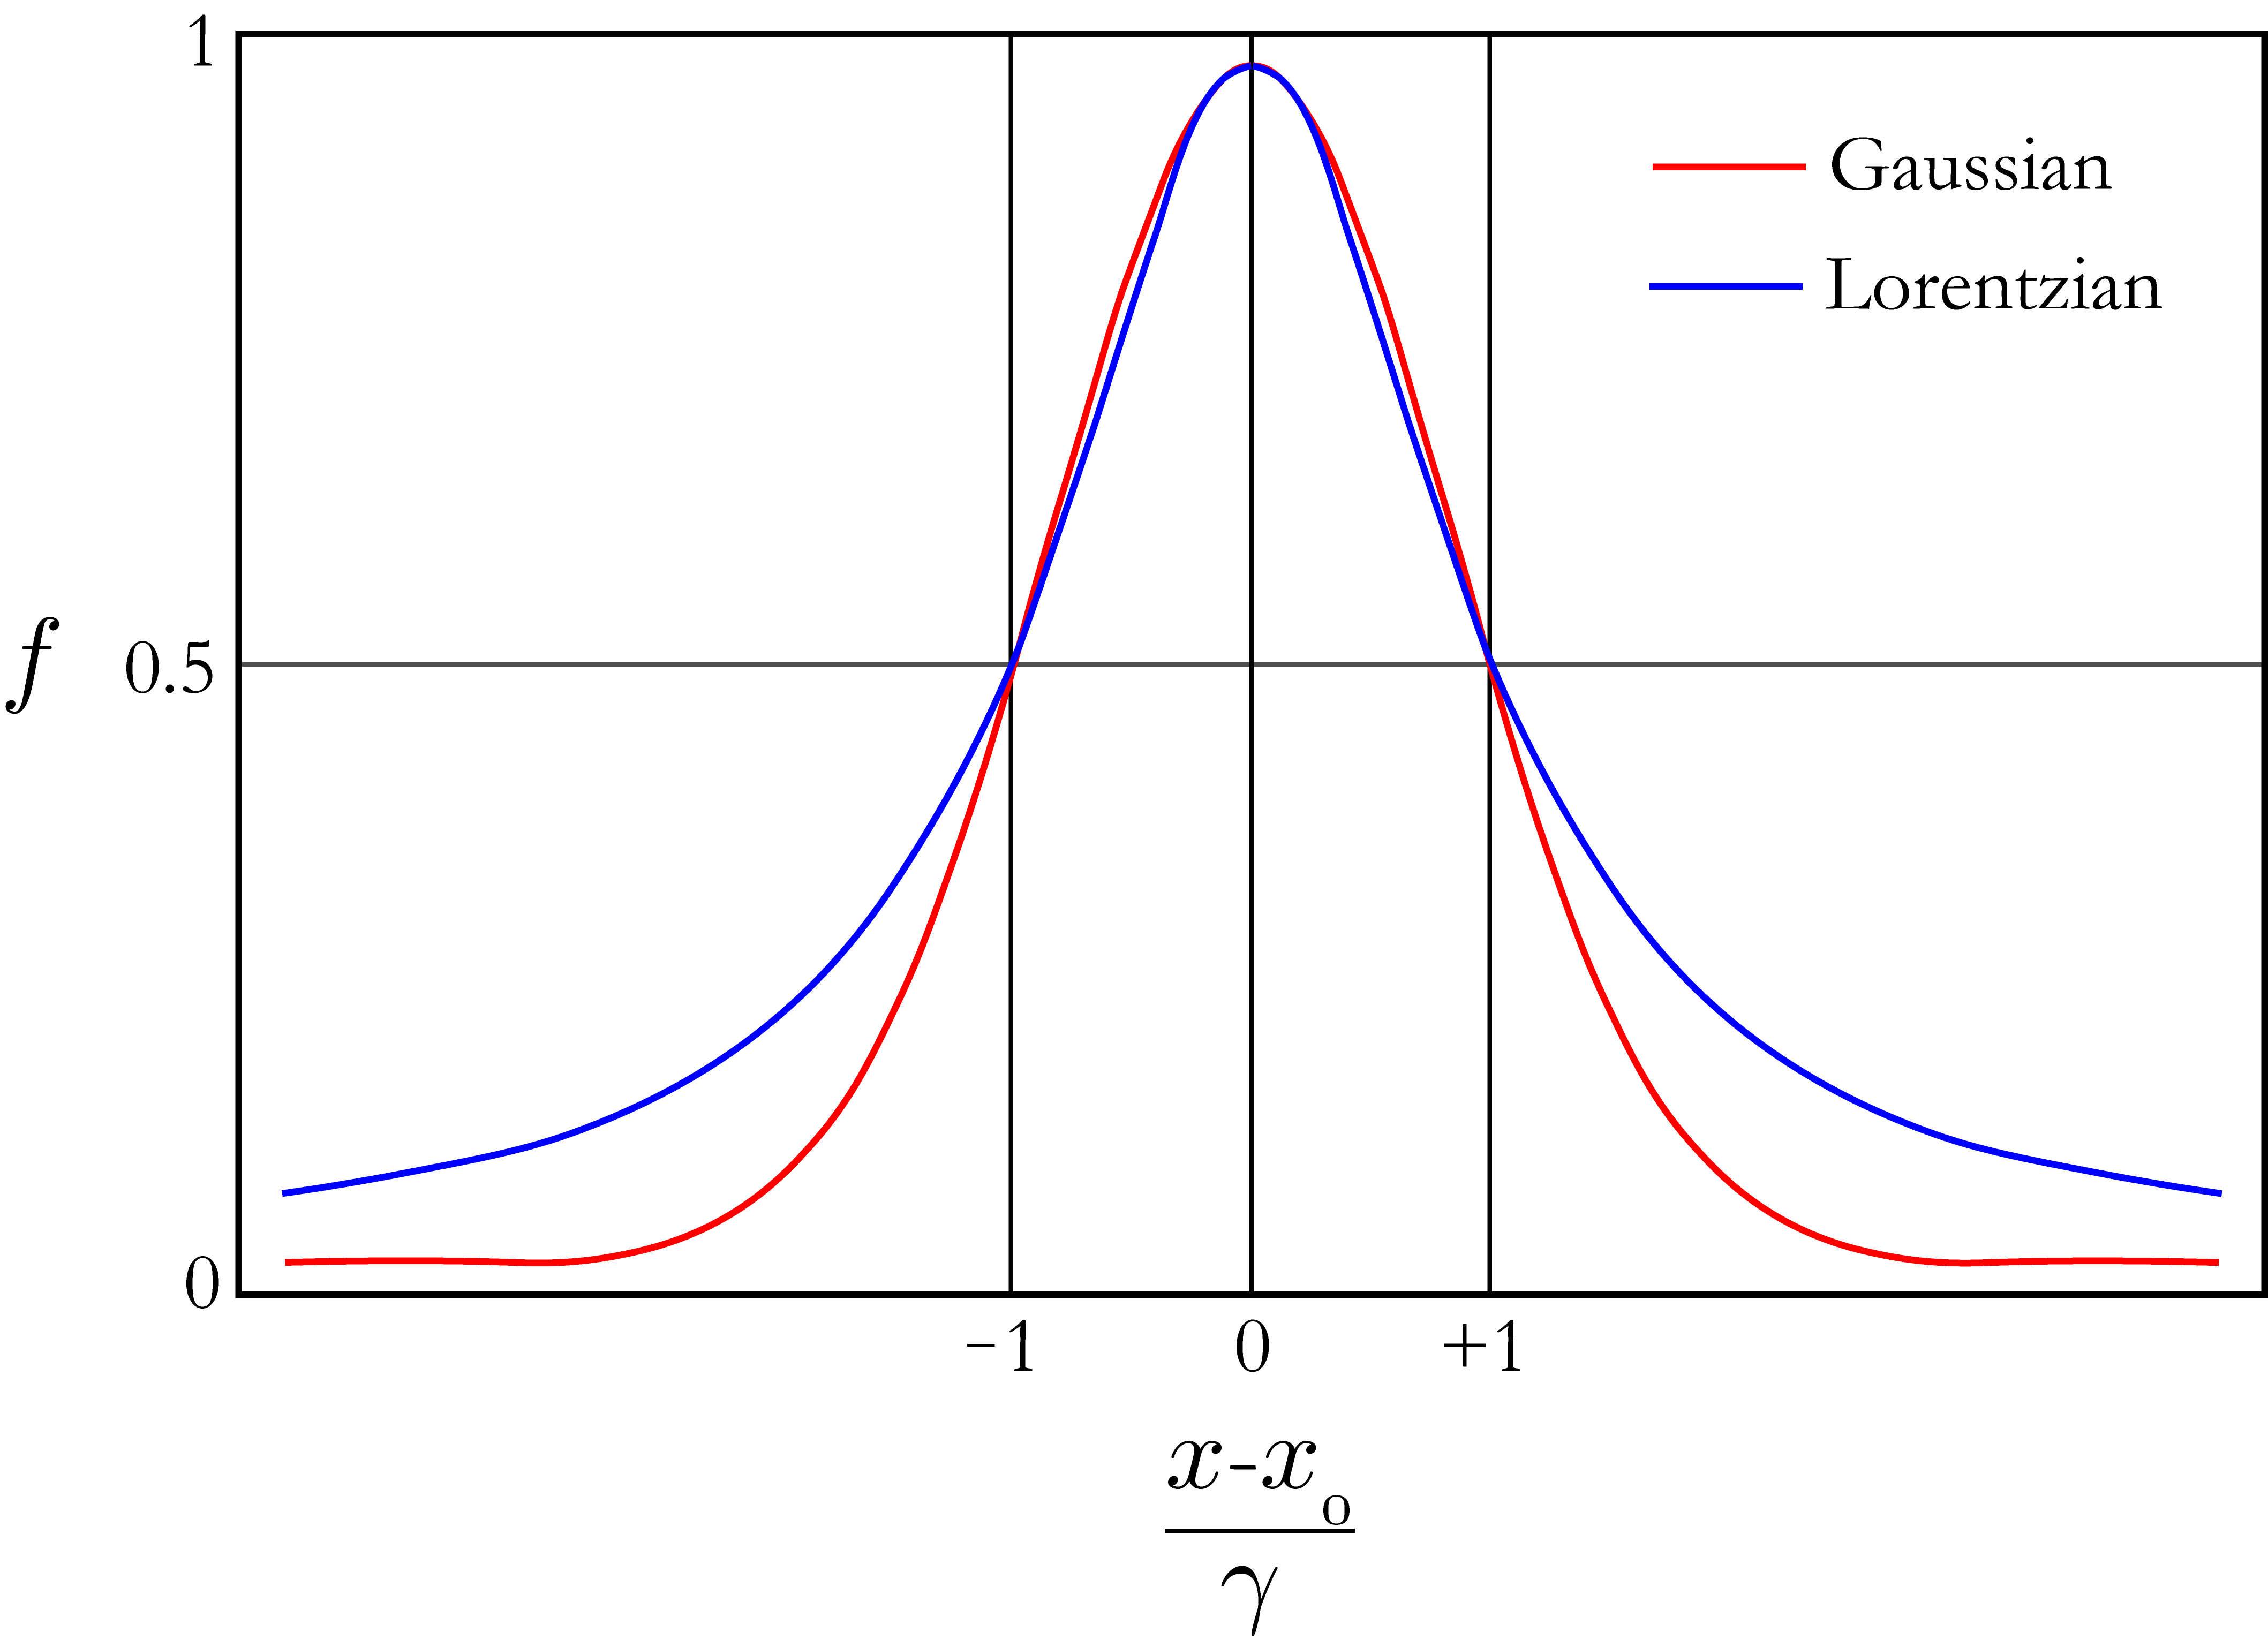
\includegraphics[width=10cm]{image/6-3-5.png}
\caption{高斯型和洛伦兹型\protect\footnotemark}

\end{figure}

\footnotetext{高斯型是指高斯分布:
\[{\rm pdf.}=\frac{1}{\sqrt{2\pi}\sigma}\ue^{-\frac{(x-x_0)^2}{2\sigma^2}}\]}

这样一个分布函数是需要有归一化的要求的:
\[\int_{-\infty}^{+\infty}{\rm pdf. }\,\ud x=1\]

但是现在的幅频特性,\,明显与洛伦兹型是有出入的.\,第一是,\,我们需要把因变量修改为$I=|A|^2$而不是$|A|$.\,这代表振动的强度而不是振幅.\,第二是,\,不同于柯西分布的分母为二次函数,\,这里的分母却作为了$x$的四次函数.\.也是$\omega$的四次函数.\,虽然$I(\omega)$与柯西分布有别,\,而且也不归一化.\,但是却体现出类似的性质.\,它们都是有一个峰,\,并在峰两侧按照较慢的多项式的方式衰减(而不是像高斯型那样指数衰减).\,而且我们都用\emph{半高峰宽}(FWHM,\,full width at half maximum)来描述峰的宽度.\,它被定义为函数值,\,或者代表的强度减少为峰值的一半对应的两点之间的区间宽度.\,对于标准的洛伦兹型,\,容易发现半高峰宽就是:
\[{\rm FWHM}=2\gamma\]

谐振子的幅频曲线的半高峰宽就更加难算.\,我们此时会采取一个近似技巧,\,不难验证其正确性.\,注意到在洛伦兹型中取到半高的点处分母中的两项是相等的,\,于是有理由相信在$I(x)$函数情况下,\,直接让分母两项相等就也近似是在半高点处:
\[I(x)=I_0\left/\middle[(1-x^2)^2+\frac{x^2}{Q^2}\right]\quad\Rightarrow\quad I_{\rm max}\approx I_0\]
\[I=\frac{I_{\rm max}}{2}\quad\Rightarrow\quad 1-x^2\approx \pm\frac{x}{Q}\]

这就可以确定,\,取到半高的点$x_+,\,x_-$为:
\[x_+=\sqrt{1+\frac{1}{4Q^2}}+\frac{1}{2Q}\quad;\quad x_-=\sqrt{1+\frac{1}{4Q^2}}-\frac{1}{2Q}\quad\Rightarrow \quad x_+-x_-=\frac{1}{Q}\]



而$\omega_+=x_+\omega_0,\,\omega_-=x_-\omega_0$.\,从而半高峰宽就是:
\[{\rm FWHM}=\Delta\omega=\omega_+-\omega_-=\frac{\omega_0}{Q}\]

我们又发现了品质因数的一种常见定义方式,\,它被定义为谱线的\emph{锐度}(sharpness),\,即峰处角频率与半高峰宽的比值:
\[Q=\frac{\omega_0}{\Delta \omega}\]





\section{多自由度小振动*}

多自由度小振动,\,首先得是一个多自由度平衡问题.\,在上一章带约束的完整系统的静力学平衡的基础上.\,如果体系还存在$f$个自由度,\,与之对应的有$f$个广义坐标$q_i$.\,那么我们指出过,\,体系的平衡条件为:
\[Q_i=\sum_k \bs{F}_k\cdot \frac{\partial \bs{r}_k}{\partial q_i}=0\]

但是在绝大多数情况下,\,我们处理的是保守体系的问题.\,所以这种场合下又有势能函数$V(q_i)$.\,广义力也能从势能中得到:
\[Q_i=\frac{\partial V}{\partial q_i}\]

这完全就能得到保守体系的平衡条件:
\[\frac{\partial V}{\partial q_i}=0\]

又是在绝大多数情况下,\,势能函数是性质非常良好的函数\footnote{数学上叫做光滑函数.}.\,从而可以在平衡位置附近泰勒展开.\,把平衡位置记作$q_{i0}$,\,而偏离平衡位置的位移为$\delta_i$,\,平衡位置处势能记作$V_0=V(q_{i0})$,\,由于平衡位置一阶导数为零,\,故:
\[V(q_{i0}+\delta_i)=V_0+\frac{1}{2}\sum_{i,\,j}\left.\frac{\partial^2 V}{\partial q_i\partial q_j}\right|_{q_{i0}}\delta_i\delta_j+\frac{1}{3!}\sum_{i,\,j,\,k}\left.\frac{\partial^3 V}{\partial q_i\partial q_j\partial q_k}\right|_{q_{i0}}\delta_i\delta_j\delta_k+\cdots\]

在忽略三阶小量(不会成为领头项,\,条件下面再讨论)的前提下,\,再通过去掉常数$V_0$,\,不影响势能的效果.\,我们发现势能实际上就成为了一个二次型:
\[V=\frac{1}{2}\sum_{i,\,j}\left.\frac{\partial^2 V}{\partial q_i\partial q_j}\right|_{q_{i0}}\delta_i\delta_j=\frac{1}{2}\sum_{i,\,j} V_{ij}\delta_i\delta_j\]

而动能,\,由于在平衡位置附近小范围内做小的运动,\,当然也是一个关于广义速度的二次型,\,系数为常数$T_{ij}$:
\[T=\frac{1}{2}\sum_{i,\,j} T_{ij}\dot{\delta}_i\dot{\delta}_j\]

关于系数$T_{ij},\,V_{ij}$.\,一个要求是它们必须对称:
\[T_{ij}=T_{ji}\quad;\quad V_{ij}=V_{ji}\]

其中的道理非常简单,\,例如只有两个广义坐标的变化$\delta_1,\,\delta_2$.\,那么$V_{12}=a\neq V_{21}=b$所决定的势能二次型与$V_{12}=V_{21}=(a+b)/2$决定的二次型根本就是同一个:
\[V_{12}=a\neq V_{21}=b:\,V=\frac{1}{2}V_{11} \delta_1^2+\frac{1}{2}V_{22} \delta_2^2+\frac{1}{2}a\delta_1\delta_2+\frac{1}{2}b\delta_2\delta_1=\frac{1}{2}V_{11} \delta_1^2+\frac{1}{2}V_{22} \delta_2^2+\frac{1}{2}(a+b)\delta_1\delta_2\]
\[V_{12}=V_{21}=\frac{a+b}{2}:\,V=\frac{1}{2}V_{11} \delta_1^2+\frac{1}{2}V_{22} \delta_2^2+\frac{1}{2}\frac{a+b}{2}\delta_1\delta_2+\frac{1}{2}\frac{a+b}{2}\delta_2\delta_1=\frac{1}{2}V_{11} \delta_1^2+\frac{1}{2}V_{22} \delta_2^2+\frac{1}{2}(a+b)\delta_1\delta_2\]

反过来,\,如果给一个二次型,\,我们也中总可以把系数写成对称的形式,\,比如在动能中,\,毕竟偏导数本身也是可交换次序的:
\[T_{ij}=\frac{\partial^2 T}{\partial \dot{\delta}_i\partial \dot{\delta}_j}=\frac{\partial^2 T}{\partial \dot{\delta}_j\partial \dot{\delta}_i}=T_{ji}\]

\begin{wrapfigure}[38]{o}[-10pt]{6cm}
\centering
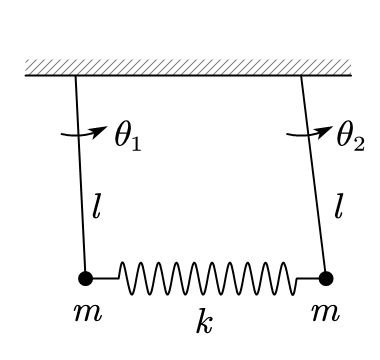
\includegraphics[width=6cm]{image/6-3-7.png}
\caption{耦合摆}\label{6-3-6}
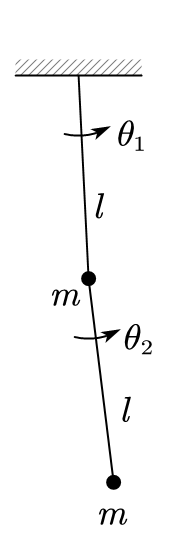
\includegraphics[width=2.5cm]{image/6-3-6.png}
\caption{双摆}\label{6-3-7}
\end{wrapfigure}
举两个例子.\,在\emph{耦合摆}(coupled pendulum)问题\ref{6-3-6}中,\,分开看是相同的两个单摆,\,但却因为弹簧而发生弱的耦合,\,设想弹簧原长为$x$为摆间距,\,这样就使得两单摆按原来的位置平衡时,\,弹簧也没有作用力.\,但只要一发生运动就彼此影响,\,设两摆球距离$x'=\sqrt{(x+l\sin\theta_2-l\sin\theta_1)^2+(l\cos\theta_2-l\cos\theta_1)^2}$.\,这样作为整体体系动能和势能为:
\[T_{\rm cp}=\frac{1}{2}ml^2\dot{\theta}_1^2+\frac{1}{2}ml^2\dot{\theta}_2^2\]
\[V_{\rm cp}=mgl(1-\cos\theta_1)+mgl(1-\cos\theta_2)+\frac{1}{2}k(x'-x)^2\]

再引入描述耦合强度的参量$\varepsilon=kl/mg$,\,小量近似以后,\,动能,\,势能被近似为二次型:
\[T_{\rm cp}=\frac{1}{2}\cdot ml^2\cdot \dot{\theta}_1^2+\frac{1}{2}\cdot ml^2\cdot \dot{\theta}_2^2\]
\[V_{\rm cp}=\frac{1}{2}\cdot (1+\varepsilon)mgl\cdot{\theta}_1^2+\frac{1}{2}\cdot (1+\varepsilon)mgl\cdot{\theta}_2^2-\varepsilon mgl\cdot {\theta}_1{\theta}_2\]

而在\emph{双摆}(double pendulum)问题\ref{6-3-7}中,\,两个摆直接悬挂在一起.\,也会彼此影响.\,体系动能和势能为:
\[T_{\rm dp}=\frac{1}{2}ml^2\dot{\theta}_1^2+\frac{1}{2}ml^2[\dot{\theta}_1^2+\dot{\theta}_2^2+2\dot{\theta}_1\dot{\theta}_2\cos(\theta_1-\theta_2)]\]
\[V_{\rm dp}=mgl(1-\cos\theta_1)+mgl(1-\cos\theta_1)+mgl(1-\cos\theta_2)\]


小量近似以后,\,动能,\,势能被近似为二次型:
\[T_{\rm dp}=\frac{1}{2}\cdot 2ml^2\cdot\dot{\theta}_1^2+\frac{1}{2}\cdot ml^2\cdot\dot{\theta}_2^2+ml^2\cdot\dot{\theta}_1\dot{\theta}_2\]
\[V_{\rm dp}=\frac{1}{2}\cdot 2mgl\cdot{\theta}_1^2+\frac{1}{2}\cdot mgl\cdot{\theta}_2^2\]

如果把$T_{ij}$和$V_{ij}$写成矩阵,\,那么对应的矩阵叫做\emph{惯性矩阵}(inertial matrix)和\emph{弹性矩阵}(elastic matrix):
\[[T_{ij}]_{\rm cp}=ml^2\begin{bmatrix} 1&0\\ 0&1\end{bmatrix}\quad;\quad [V_{ij}]_{\rm cp}=mgl \begin{bmatrix} 1+\varepsilon&-\varepsilon\\ -\varepsilon &1+\varepsilon\end{bmatrix}\]
\[[T_{ij}]_{\rm dp}=ml^2\begin{bmatrix} 2&1\\ 1&1\end{bmatrix}\quad;\quad [V_{ij}]_{\rm dp}=mgl \begin{bmatrix} 2&0\\ 0&1\end{bmatrix}\]

从而我们可以发现这两个问题的重大区别在于,\,前一个问题动能规整,\,势能却具有交叉项.\,后一个问题势能规整,\,动能却具有交叉项.

当我们遇到一个这样普遍的小振动问题时,\,该如何得到其运动的特征.\,有两种常见的做法:\,一是通过换元来实现动能势能的简化,\,这种方法需要较深厚的数学基础,\,又最好通过拉格朗日方程来理解一些过程.\,我们下面也写出具体的过程,\,有兴趣的读者可以做进一步研究;\,但也有第二种简易的方法来求解一些直接的量.\,我们也在详细讨论的方法之后加上去:

\subsection{基于线性代数与分析力学的简正坐标求解}

对一个任意的二次型进行配方并不是难事.\,例如$F(x_1,\,x_2\cdots)$是一个二次型,\,那么它必然可以写作:
\[F(x_1,\,x_2\cdots)=\frac{1}{2}f_{11}x_1^2+x_1(f_{12}x_2+f_{13}x_3+\cdots)+(\frac{1}{2}f_{22}x_2^2+\cdots)\]

即$x_1$自己的项,\,和别的变量``耦合''的项以及与$x_1$无关的项.\,那么做变量代换:
\[x_1'=x_1+\frac{f_{12}}{f_{11}}x_2+\frac{f_{13}}{f_{11}}x_3+\cdots\]

便可以把``耦合''项配方到$x_1$自己的项内,\,上式变成:
\[F(x_1,\,x_2\cdots)=\frac{1}{2}f_{11}x_1'^2+F'(x_2,\,x_3\cdots)\]

之后只要继续对$F'$配方,\,每次可以得到一个完全平方的项,\,余项则是剩下的变量的二次型,\,变量数至少减一.\,这样就可以实现任意二次型的完全配方.\,用这个方法可以选择动能或者势能进行化简.\,最终形式,\,由上讨论,\,只包含平方项,\,没有交叉项.\,由于这样对应的矩阵是对角矩阵.\,我们把这样的配方过程称作\emph{对角化}(diagonalization):
\[T=\sum_i\frac{1}{2}T_i \dot{\delta}_i^2\quad ;\quad V=\sum_i\frac{1}{2}V_i \delta_i^2\]

注意这里动能和势能的对角化是分开来进行的.\,对应的系数$T_i$叫做\emph{惯性系数}(inertial coefficient),\,而$T_i$叫做\emph{弹性系数}(elastic coefficient).\,同时我们对这些系数必然有以下期待:

\begin{itemize}
	\item 动能的对角化结果:
		\begin{itemize}
			\item 非退化正定二次型:\,所有$T_i>0$.
			\item 退化正定二次型:\,个别$T_i=0$.
			\item 不可能出现某个$T_i<0$.
		\end{itemize}
	\item 势能的对角化结果:
		\begin{itemize}
			\item 非退化正定二次型:\,所有$V_i>0$.
			\item 可以负的二次型:\,存在$V_i<0$.
			\item 退化的二次型:\,所有$V_i\geq 0$且也存在$V_i= 0$.
		\end{itemize}
\end{itemize}

说明:

动能不可以出现负的惯性系数,\,是因为在所有情况下动能都必须大于零.\,但是在有的情况下惯性系数可以为零,\,即,\,即使广义速度不为零,\,造成的动能为零,\,称作\emph{退化}(degenarate)的情况.\,这要么说明体系存在没有动力学效果的冗余自由度.\,例如无限细的杆的自转角就是这样的例子.\,去掉这个广义坐标也不影响能量的表达式.\,要么说明这个自由度上的动能是一个高阶小量.\,只是在目前平衡位置,\,系数``偶然''地等于了零,\,只要偏离这个位置去振动就会产生一定的动能,\,抑或我们在实际问题中需要考虑更高阶泰勒展开产生的广义速度的高次项.\,后面这种情况一般就与简谐振动无关了.\,再次不予考虑.\,故我们此后做假设:\,\emph{所有小振动问题,\,动能必须是非退化正定的.}

势能就更加复杂.\,势能相对平衡位置本来就可正可负.\,那么上面我们分为三种情况其实就包括了所有情况.\,有一点是非常突出的,\,如果沿某方向偏离平衡位置时,\,势能降低了,\,那么原平衡位置就一定是\emph{非稳定平衡}(unstable equilibrium).\,在仅仅考虑二次型的情况下,\,一旦出现一个负的弹性系数这就成为了必然.\,但是即使一个负的弹性系数都没有,\,也不能因此就下断言原位置是稳定的.\,因为还有二次型\emph{退化}的情况.\,它发生在某些弹性系数为零时,\,此时高阶泰勒展开项如果是负的,\,它依然可以不稳定,\,普遍情况得考察多个领头项.\,但是,\,有一点很好判断:\,就是如果所有弹性系数为正,\,那么原来的位置就一定是\emph{稳定平衡}(stable equilibrium).\,因为此时任意的偏离平衡位置都使得势能升高.\,也只有稳定平衡才能作为小振动问题求解的先决条件.\,故我们此后做假设:\,\emph{所有小振动问题,\,势能必须是非退化正定的.}

但是虽然单独对动能或势能对角化简单,\,但是两者却不会同时对角化.\,例如在双摆问题中,\,对于动能:
\[T_{\rm dp}=\frac{1}{2}\cdot 2ml^2\cdot\dot{\theta}_1^2+\frac{1}{2}\cdot ml^2\cdot\dot{\theta}_2^2+ml^2\cdot\dot{\theta}_1\dot{\theta}_2=\frac{1}{2}\cdot 2ml^2\cdot\left(\dot{\theta}_1+\frac{1}{2}\dot{\theta}_2\right)^2+\frac{1}{2}\cdot \frac{ml^2}{2}\cdot\dot{\theta}_2^2\]

但是如果做换元$\vartheta_1=\theta_1+\theta_2/2,\,\vartheta_2=\theta_2$,\,动能倒是没有交叉项了,\,但原来好好的势能又产生交叉项了:
\[V_{\rm dp}=\frac{1}{2}\cdot 2mgl\cdot{\vartheta}_1^2+\frac{1}{2}\cdot \frac{3}{2}mgl\cdot{\vartheta}_2^2-mgl\cdot {\vartheta}_1{\vartheta}_2\]

所以,\,我们这里要追求的其实是\emph{同时对角化}(simutalneous diagonalization)的技巧.\,为了进一步研究,\,我们先来抽象对角化的过程.\,根据矩阵理论,\,任何一个坐标变换,\,其实是一个线性变换:
\[[q_i']=[A_{ij}][q_j]\]

这个式子是以下两种写法的缩略形式:
\[q_i'=\sum_j A_{ij}q_j\quad {\rm or}\quad \begin{bmatrix}q_1'\\q_2'\\ \vdots\\ q_n'\end{bmatrix}=\begin{bmatrix}A_{11}&A_{12}&\cdots&A_{1n}\\ A_{21}&A_{22}&\cdots &A_{2n}\\ \vdots&\vdots &&\vdots\\ A_{n1}&A_{n2}&\cdots &A_{nn} \end{bmatrix}\begin{bmatrix}q_1\\q_2\\ \vdots\\ q_n\end{bmatrix}\]

它的逆变换:\,求出$[A_{ij}]$的逆矩阵$[B]_{ij}$,\,就可以用新坐标表示旧坐标:
\[[q_i]=[B_{ij}][q_j']\]

而动能,\,势能都可以用矩阵来表示\footnote{用$\phantom{}^{\rm t}[q_i]$表示转置,\,即把列向量写作行向量.}:
\[T=\frac{1}{2}\phantom{}^{\rm t}[\dot{q}_i][T_{ij}][\dot{q}_j]\quad ;\quad V=\frac{1}{2}\phantom{}^{\rm t}[q_i][V_{ij}][q_j]\]

这样只要把之前的变换代入这两个二次型,\,就得到了变换之后的二次型:
\[T=\frac{1}{2}\phantom{}^{\rm t}[\dot{q}'_i]\phantom{}^{\rm t}[B_{ij}][T_{jk}][B_{kl}][\dot{q}'_l]=\frac{1}{2}\phantom{}^{\rm t}[\dot{q}'_i][T'_{il}][\dot{q}'_l]\]
\[V=\frac{1}{2}\phantom{}^{\rm t}[q'_i]\phantom{}^{\rm t}[B_{ij}][V_{jk}][B_{kl}][q'_l]=\frac{1}{2}\phantom{}^{\rm t}[q'_i][V'_{il}][q'_l]\]

这说明其实在坐标变换以后,\,惯性和弹性矩阵是按照右乘一个矩阵,\,再左乘它的转置来进行的.\,这种对矩阵的变换数学上叫做\emph{合同变换}(congruent transformation):
\[[T'_{il}]=\phantom{}^{\rm t}[B_{ij}][T_{jk}][B_{kl}]\quad ;\quad [V'_{il}] =\phantom{}^{\rm t}[B_{ij}][V_{jk}][B_{kl}]\]

要把$[T]$和[V]同时对角化,\,其实问题的诀窍是求解\emph{本征值问题}(eigenvalue problem):
\[([V_{ij}]+\lambda [T_{ij}])[x_j]=[0]\]

即,\,确定是否存在常数$\lambda$\footnote{后面会知道一定非零.}和非零向量$[x_j]$使得两个矩阵组合以后恰好作为系数使得这个向量作为以上方程的解.\,乍一看这似乎很抽象.\,其实这背后的物理意义可以做这样的理解:\,既然是小振动,\,就有可能找到一些简单的运动模式,\,此时所有坐标上都是做不同振幅的简谐振动,\,即:
\[[q_i]=[x_i]\cos\omega t\]




如何写出这种情况下的动力学方程?\,一种完全严谨的做法就是利用上一章讨论的拉格朗日方程:
\[L=T-V=\frac{1}{2}\phantom{}^{\rm t}[\dot{q}_i][T_{ij}][\dot{q}_j]-\frac{1}{2}\phantom{}^{\rm t}[q_i][V_{ij}][q_j]\]

\[\frac{\ud }{\ud t}\frac{\partial L}{\partial \dot{q}_i}=\frac{\partial L}{\partial {q}_i}\quad\Rightarrow \quad [T_{ij}][\ddot{q}_j]=-[V_{ij}][q_j]\]

将简谐振动解带入,\,就得到了:
\[([V_{ij}]-\omega^2 [T_{ij}])[x_j]=[0]\]

从而原来的本征值问题中的$\lambda$代表的含义就是振动角频率平方$\omega^2$.\,那么这个本征值问题又如何求解?\,首先,\,上式中方程组存在解且非零的条件为系数行列式为零:
\[{\rm det}([V_{ij}]-\lambda [T_{ij}])=0\]

这就构成了关于$\lambda$的$n$次方程,\,他就一定有$n$个根,\,不过可以有重根.\,把这$n$个根带入,\,我们就可以把对应的$n$个本征向量\footnote{注意本征向量的存在性,\,非重根是显然的,\,但是如果有个$s$重根,\,是否也有$s$组独立的解向量?\,这不是显然的,\,需要证明,\,在次略去.\,一般线性代数的教材上都会有证明方法,\,不过一般会默认是$[T_{ij}]$为单位矩阵的简单情况,\,其实这不影响证明过程.}$[x_j]$找到,\,这仅仅是个体力活:\,求解至多$n$次$n$元线性方程组.\,一旦求解完毕,\,我们就找到了$n$个$\lambda$和$n$个$[x_j]$,\,可以记作:
\[([V_{ij}]-\lambda_k [T_{ij}])[B_{j,k}]=[0]\]

最后还需证明一点,\,就是这$k=1,\,2\cdots n$个本征值对应的本征向量不仅是独立的,\,而且还是\emph{正交}(orthogonal)的.\,注意这里的正交是指:
\[k\neq k'\quad\Rightarrow\quad\phantom{}^{\rm t}[B_{i,k}][T_{ij}][B_{j,k'}]=0\]

这个正交性足以说明独立性,\,毕竟如果$[B_{i,k}]$与$[B_{i,k'}]=0$不独立,\,那么前者(非零)就是后者(非零)的常数(非零)倍,\,以上$\phantom{}^{\rm t}[B_{i,k}][T_{ij}][B_{j,k'}]$就会变成常数乘以后者产生的动能,\,显然是非零的.\,所以一旦上式为零,\,两个矢量正交就足以说明它们不会同向.

证明正交性的依据还是它们的定义.\,首先我们发现,\,如果任意两个矢量恰好成为不同本征值下的本征向量:
\[([V_{ij}]-\lambda_1 [T_{ij}])[x_{j,1}]=[0]\;,\;([V_{ij}]-\lambda_2 [T_{ij}])[x_{j,2}]=[0]\quad,\quad \lambda_1\neq\lambda_2\]

构造式子$\phantom{}^{\rm t}[x_{i,1}][V_{ij}][x_{j,2}]$.\,一方面先计算前面的向量乘弹性矩阵,\,一方面也可以先算后面的向量乘弹性矩阵:
\[\phantom{}^{\rm t}[x_{i,1}][V_{ij}]=\lambda_1\phantom{}^{\rm t}[x_{i,1}][T_{ij}]\quad,\quad [V_{ij}][x_{j,2}]=\lambda_2[T_{ij}][x_{j,2}]\]
\[\Rightarrow \quad \phantom{}^{\rm t}[x_{i,1}][V_{ij}][x_{j,2}]=\lambda_1\phantom{}^{\rm t}[x_{i,1}][T_{ij}][x_{j,2}]=\lambda_2\phantom{}^{\rm t}[x_{i,1}][T_{ij}][x_{j,2}]\]
\[\lambda_1\neq \lambda_2 \quad\Rightarrow\quad [x_{i,1}][T_{ij}][x_{j,2}]=0\]

这实际上是证明了,\,由$n$个本征向量$[B_{i,k}]$形成的空间根据不同的本征值彼此正交,\,即使在某个本征值下有多个本征向量,\,总可以在它们线性组合形成的空间中选取相互正交的向量作为本征向量.\,这样我们就得到了一组特殊的本征向量,\,它们符合:
\[\phantom{}^{\rm t}[B_{i,k}][T_{ij}][B_{j,k'}]=0\quad{\rm if}\quad k\neq k'\]

而当$k=k'$时上述值一定大于零,\,这些结果,\,后面就可以看到,\,其实就是惯性系数:
\[\phantom{}^{\rm t}[B_{i,k}][T_{ij}][B_{j,k}]=T_k\]

现在我们直接把这$n$个$n$行的列向量横向按顺序并置构成矩阵:
\[[B_{ij}]=[[B_{i,\,1}]\,,\,[B_{i,\,2}]\cdots [B_{i,\,n}]]\]

这样以上关系其实就表示为了:
\[\phantom{}^{\rm t}[B_{ij}][T_{jk}][B_{kl}]=\mathfrak{Diag}(T_i)\]

其中$\mathfrak{Diag}(T_i)$表示由$T_i$作为元素的对角矩阵.\,同理我们如果考察弹性矩阵,\,也有:
\[\phantom{}^{\rm t}[B_{i,k}][V_{ij}][B_{j,k'}]=0\quad{\rm if}\quad k\neq k'\]
\[\phantom{}^{\rm t}[B_{i,k}][V_{ij}][B_{j,k}]=\lambda_k T_k=\omega_k^2T_k=V_k\]

同理用矩阵表示:
\[\phantom{}^{\rm t}[B_{ij}][V_{jk}][B_{kl}]=\mathfrak{Diag}(V_i)\]

这样我们之前的愿望就实现了,\,即动能矩阵与势能矩阵的同时对角化.

\vspace{1cm}

让我们来对双摆体系利用上述套路来求解:\,首先是对应的本征值问题的系数行列式为零:
\[[V]_{ij}=mgl\begin{bmatrix}2&0\\0&1\end{bmatrix}\quad;\quad [T]_{ij}=ml^2\begin{bmatrix}2&1\\1&1\end{bmatrix}\]
\[{\rm det}([V_{ij}]-\lambda [T_{ij}])=0\quad\Rightarrow\quad {\rm det}\begin{bmatrix}2g/l -2\lambda &-\lambda \\-\lambda&g/l -\lambda \end{bmatrix}=0\]
\[\Rightarrow\quad 2(g/l-\lambda)^2=\lambda^2\]

从而得到特征值:
\[\lambda_1=\omega_1^2=(2-\sqrt{2})\frac{g}{l}\quad;\quad\lambda_2=\omega_2^2=(2+\sqrt{2})\frac{g}{l}\]

带入本征值问题,\,分两个本征值来求解本征向量:
\[([V_{ij}]-\lambda_k [T_{ij}])[B_{j,k}]=0\;,\;k=1,\,2\]
\[\begin{bmatrix}2(\sqrt{2}-1)&-(2-\sqrt{2})\\-(2-\sqrt{2})&\sqrt{2}-1\end{bmatrix}\begin{bmatrix}B_{11}\\B_{21}\end{bmatrix}=\begin{bmatrix}0\\0\end{bmatrix}  \quad,\quad  \begin{bmatrix}-2(\sqrt{2}+1)&-(2+\sqrt{2})\\-(2+\sqrt{2})&-(\sqrt{2}+1)\end{bmatrix}\begin{bmatrix}B_{12}\\B_{22}\end{bmatrix}=\begin{bmatrix}0\\0\end{bmatrix}\]
\[\Rightarrow \quad \begin{bmatrix}B_{11}\\B_{21}\end{bmatrix}=\begin{bmatrix}1\\\sqrt{2}\end{bmatrix}\quad,\quad \begin{bmatrix}B_{12}\\B_{22}\end{bmatrix}=\begin{bmatrix}1\\-\sqrt{2}\end{bmatrix}\]

这就给出了一个坐标变换矩阵:
\[[B_{ij}]=\begin{bmatrix}1&1\\\sqrt{2}&-\sqrt{2}\end{bmatrix}\]

其逆矩阵:
\[[A_{ij}]=\begin{bmatrix}\frac{1}{2}&\frac{\sqrt{2}}{4}\\\frac{1}{2}&-\frac{\sqrt{2}}{4}\end{bmatrix}\]

这就是给出了如下的坐标变换:
\[\left\{\begin{array}{l}\varphi_1=\frac{1}{2}\theta_1+\frac{\sqrt{2}}{4}\theta_2\\ \varphi_2=\frac{1}{2}\theta_1-\frac{\sqrt{2}}{4}\theta_2\end{array}\right.\quad,\quad \left\{\begin{array}{l}\theta_1=\varphi_1+\varphi_2\\ \theta_2=\sqrt{2}\varphi_1-\sqrt{2}\varphi_2\end{array}\right.\]

代入便知,\,初始的动能和势能分别变为:
\[T=\frac{1}{2}\cdot 2ml^2\cdot\dot{\theta}_1^2+\frac{1}{2}\cdot ml^2\cdot\dot{\theta}_2^2+ml^2\cdot\dot{\theta}_1\dot{\theta}_2 \quad,\quad V=\frac{1}{2}\cdot 2mgl\cdot{\theta}_1^2+\frac{1}{2}\cdot mgl\cdot{\theta}_2^2\]
\[\Rightarrow \quad T=\frac{1}{2}\cdot 2(2+\sqrt{2})ml^2\cdot \dot{\varphi}_1^2+\frac{1}{2}\cdot 2(2-\sqrt{2})ml^2\cdot \dot{\varphi}_2^2\quad,\quad V=\frac{1}{2}\cdot 4mgl\cdot \varphi_1^2+\frac{1}{2}\cdot 4mgl\cdot \varphi_2^2\]

这就可以看作两个独立的振子,\,完成了\emph{解耦}(decouple).\,各自的角频率为:
\[\omega_1=\sqrt{\frac{4mgl}{2(2+\sqrt{2})ml^2}}\quad,\quad \omega_2=\sqrt{\frac{4mgl}{2(2-\sqrt{2})ml^2}}\]

与之前本征值确定的角频率是一样的.

现在我们来对这个结果产生的物理意义进行解释.\,通过坐标变换,\,我们发现动能势能形式变得简单了,\,所以新的坐标$q_i'$称作\emph{简正坐标}(normal coordinates).\,对应的频率$\omega_i$称作\emph{简正频率}(normal frequencies):
\[\omega_i=\sqrt\frac{V_i}{T_i}\quad {\rm or}\quad V_i=T_i\omega_i^2 \]

于是我们产生了一个疑问,\,为什么只要动能势能的形式变得简单,\,就可以判定体系可以等效为独立的谐振子的组合?\,其实它简单地来自于拉格朗日方程:
\[L=T-V=\sum_i\frac{1}{2}T_i(\dot{q}_i'^2-\omega_i^2q_i'^2)\]
\[\frac{\ud }{\ud t}\frac{\partial L}{\partial \dot{q}_i'}=\frac{\partial L}{\partial {q}_i'}\quad \Rightarrow \quad \ddot{q}'_i=-\omega_i^2q_i'\]

这就足以给出其解为简谐振动:
\[q_i'=C_i\cos(\omega_i t+\varphi_i)\]

再回到体系的初始广义坐标,\,它就会等于这些各自做不同频率振动的简正坐标的组合,\,从而体现出非常复杂的非简谐运动特性\footnote{要知道傅里叶理论可以证明,\,用不同频率的简谐振动组合可以无限接近任意光滑函数.}.\,具体各个广义坐标的振幅和初相位如何,\,由体系的初始条件决定.\,但是可以想象,\,存在一些简单的振动模式,\,它的初始条件决定了,\,最后只有一个简正坐标$q_k'$在做振动,\,其他的坐标振幅为零.\,那么最后原来的坐标也会具有单一的频率$\omega_k$,\,从而每一处运动都是简谐振动,\,其实它们为:
\[[q_i]=[B_{ij}][q_j']=[B_{i,\,k}]\cdot C_k\cos(\omega_k t+\varphi_k)\]

所以我们把体系以统一的频率,\,所有地方都做简谐振动的这种振动模式称作\emph{简正模}(normal mode).\,``简正''这个词语三次出现在相关术语中,\,它可以浅显地被理解为``简单''+``正确''.\,也可以更精确地被理解为``简谐''+``正交''.\,毕竟在中文语境下,\,简谐本意就是``简单''+``和谐'',\,而``正确''的``正''本身也含有方向的意味.\,英文语境下的``normal''也恰好有着异曲同工之妙.

\subsection{基于对称性的简正模判定与简正频率求解}

如何规避掉较难的数学和分析力学知识?\,用简单而优雅的方式快速确定一个多自由度简谐振动的绝大多数特征?\,我们可以采用与对称性结合的方式来求解其运动的微分方程.

就比如对于具有更好的对称性的耦合摆问题.\,我们不去追求用能量函数来解决问题,\,这样势必涉及到分析力学方法.\,而是独立地去推导两个质点的牛顿定律.\,很容易给出它们为:
\[\left\{\begin{array}{l}\ddot{\theta}_1=-\omega_0^2(1+\varepsilon)\theta_1+\omega_0^2\varepsilon\theta_2 \\ \ddot{\theta}_2=+\omega_0^2\varepsilon\theta_1-\omega_0^2(1+\varepsilon)\theta_2\end{array}\right.\]

其中$\omega_0=\sqrt{g/l}$.\,至于这个方程的求解,\,猜一个本征模解是常规操作:
\[\left\{\begin{array}{l} \theta_1=A_1\ue^{\ui\omega t}\\\theta_2=A_2\ue^{\ui\omega t} \end{array}\right.\]

但是在猜解之后,\,我们不一定要通过带入原方程,\,命系数行列式为零,\,再次带入本征频率来求解方程的曲折方程来求解振幅$A_1$和$A_2$的比.\,在本题中有一点是显然的.\,就是体系具有鲜明的左右对称性.\,这使得我们猜想:\,是不是在一种本征模式下,\,左右两个物体的位移完全相等.\,而另一个模式下,\,两个物体的位移完全相反?

这的确发生了.\,在经典物理情况下,\,这其实就对应了质心的左右振动和相对质心的二体在弹性内力下的振动.\,一般把两个物体位移相等的模式称作\emph{对称模式}(symmetric mode),\,而位移相反的模式称作\emph{反对称模式}(antisymmetric mode).\,即:
\[\left\{\begin{array}{l} \theta_{1S}=A\ue^{\ui\omega_S t}\\\theta_{2S}=A\ue^{\ui\omega_S t} \end{array}\right.\quad ,\quad \left\{\begin{array}{l} \theta_{1A}=A\ue^{\ui\omega_A t}\\\theta_{2A}=-A\ue^{\ui\omega_A t} \end{array}\right.\]

代入原来的方程就可以看出来:\,对称模式给出了:
\[-\omega_S^2A=-\omega_0^2(1+\varepsilon)A+\omega_0^2\varepsilon A\quad \Rightarrow \quad \omega_S=\omega_0\]
\[-\omega_A^2A=-\omega_0^2(1+\varepsilon)A-\omega_0^2\varepsilon A\quad \Rightarrow \quad \omega_A=\omega_0\sqrt{1+2\varepsilon}\]

可以发现,\,问题的关键在于如何看出振动模式下各个振幅之间的比例关系.\,这个问题似乎取决于问题具体的对称性.\,那么,\,何谓对称性?\,它又是怎样决定体系的振动解的.\,我们对一个更复杂的问题来做进一步研究:

\begin{figure}[H]
\centering
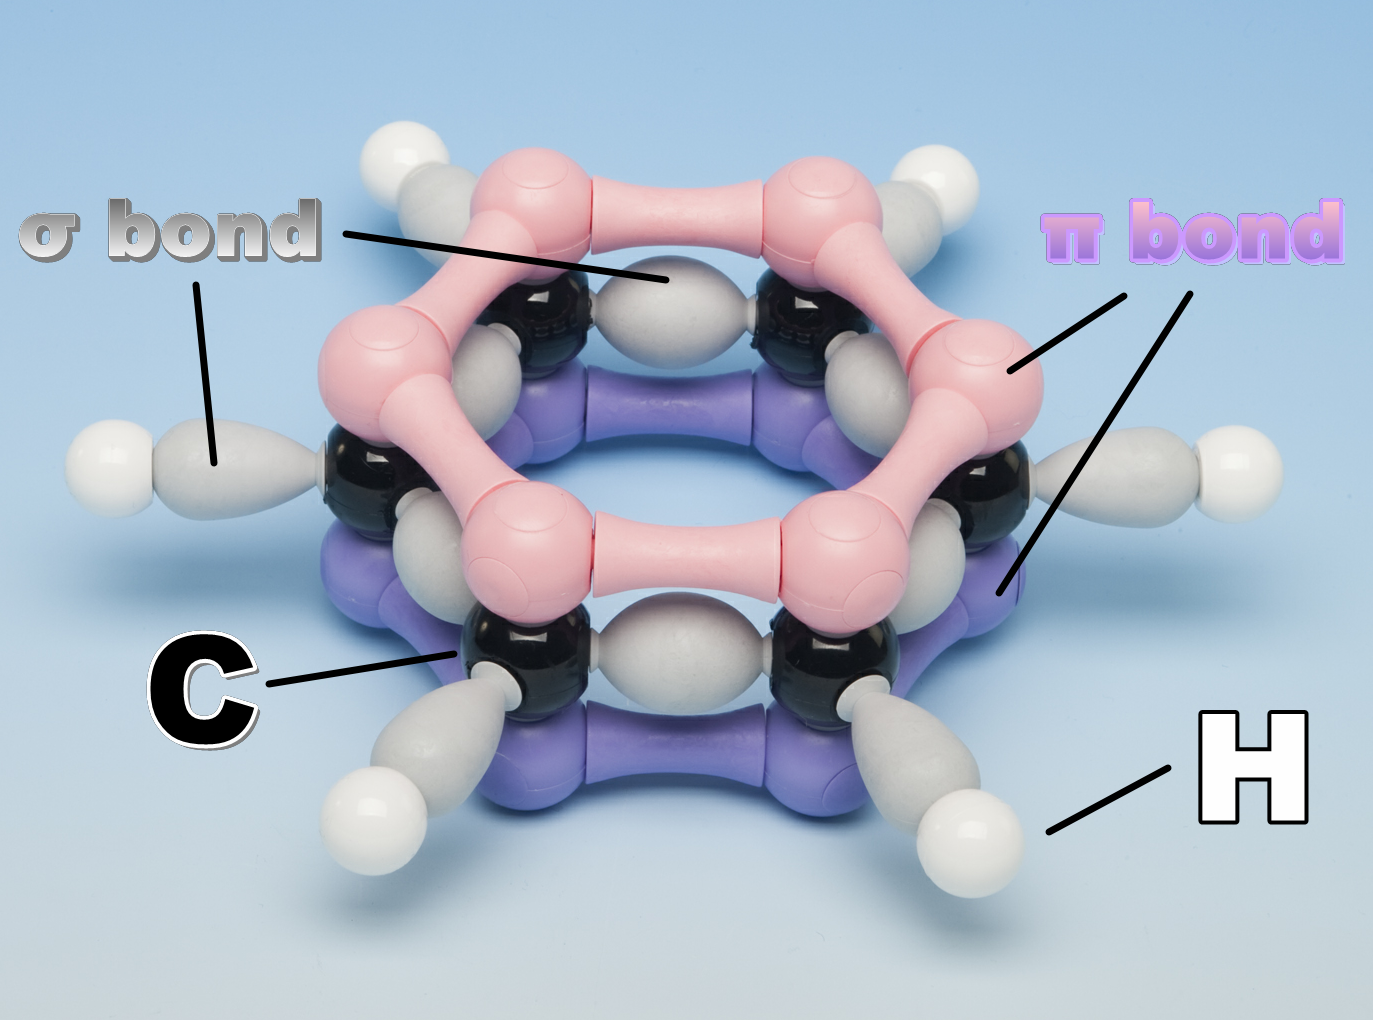
\includegraphics[width=7cm]{image/6-3-10.png}
\hspace{2cm}
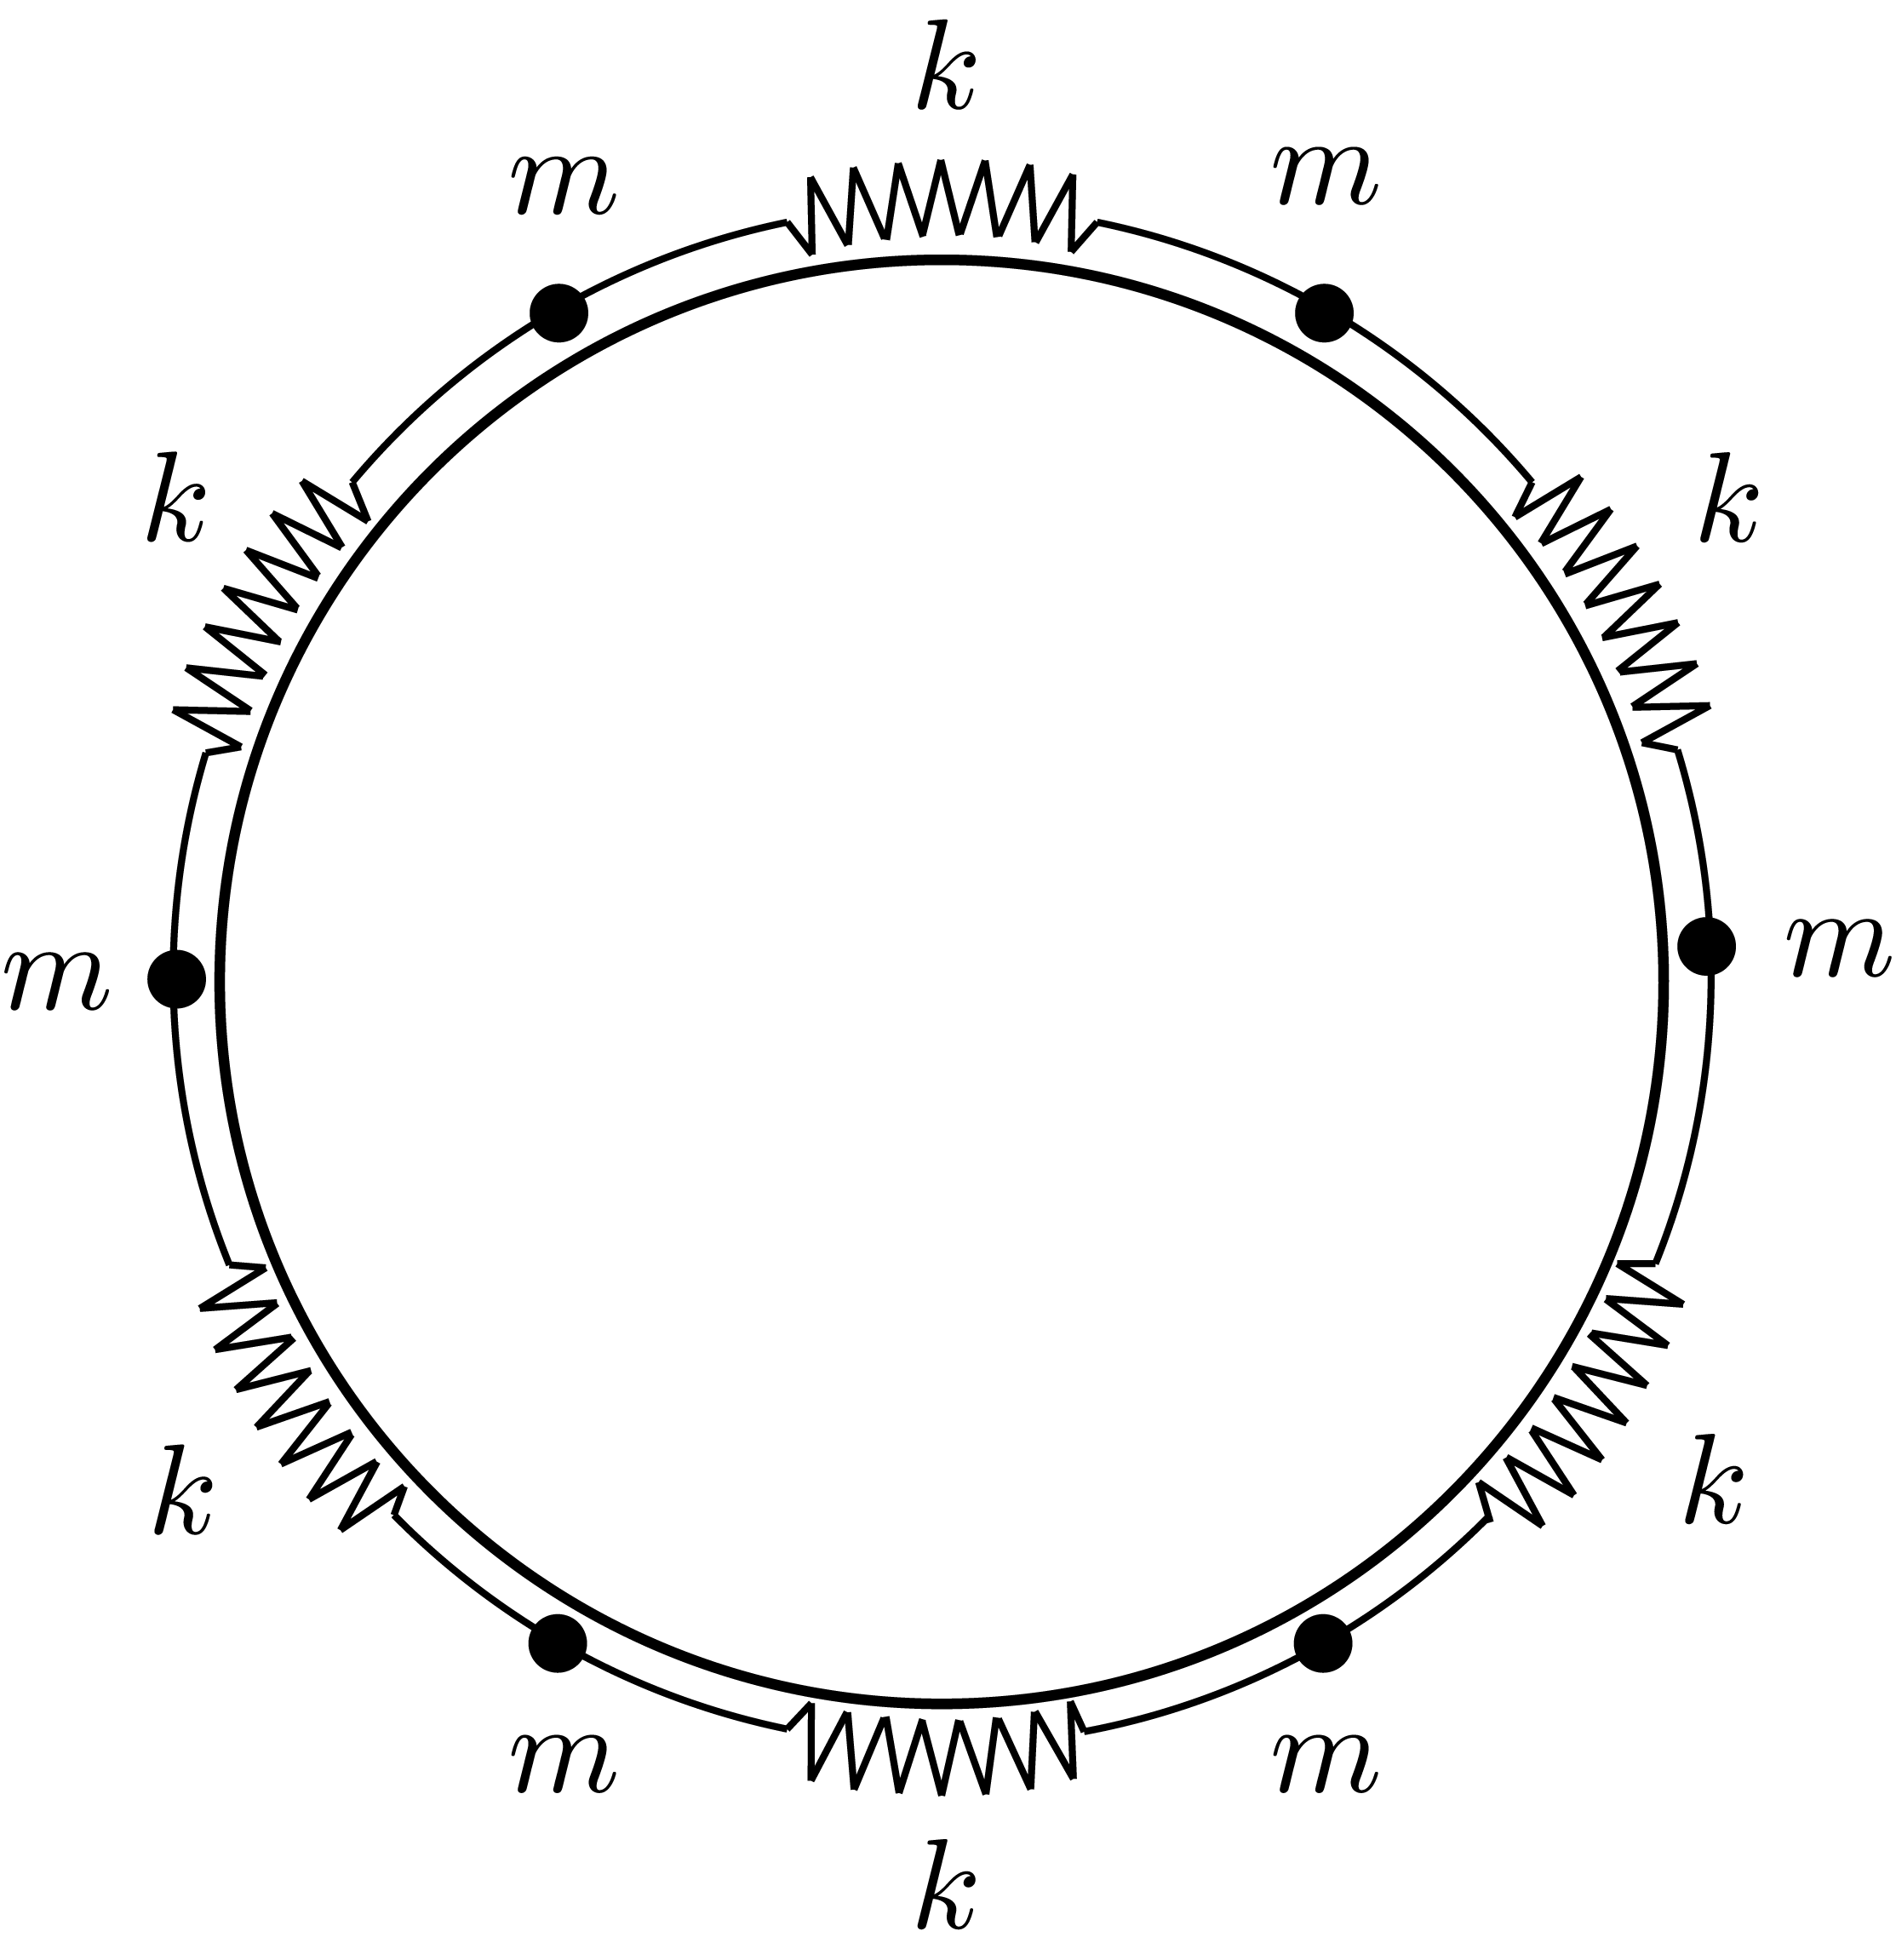
\includegraphics[width=5cm]{image/6-3-8.png}
\caption{苯: 6原子环问题}
\end{figure}

对于苯分子的振动光谱问题主要的部分就可以做如下简化:\,碳原子和氢原子作为一个整体来研究.\,设他们是在一个刚性圆环上的质量为$m$的质点.\,而彼此之间的相互作用简化为只有相邻的原子才有,\,为劲度系数为$k$的线性弹簧.\,体系还要求在一个平面上,\,甚至一个圆环上作一维运动.\,那么这个体系的能量和动力学方程为:
\[T=\sum_{i=1}^6 \frac{1}{2}m\dot{x}_i^2\quad,\quad V=\sum_{i=1}^6\frac{1}{2}m(x_{i+1}-x_i)^2\]
\[m\ddot{x}_i=-2kx_i+kx_{i+1}+kx_{i-1}\quad,\quad i=1,2\cdots 6\]

在上式中我们约定$x_0=x_6,\,x_1=x_7$.\,那么这个微分方程必然存在某种解.

我们讨论第一个问题:\,什么叫做对称性?\,表面上看上去,\,苯分子似乎具有三种对称性:\,一是绕竖直轴旋转$60^\circ$的六重轴对称性:
\[C_6:\quad x_1\to x_2,\,x_2\to x_3\,x_3\to x_4,\,x_4\to x_5,\, x_5\to x_6,\,x_6\to x_1\]

\begin{figure}[H]
\centering
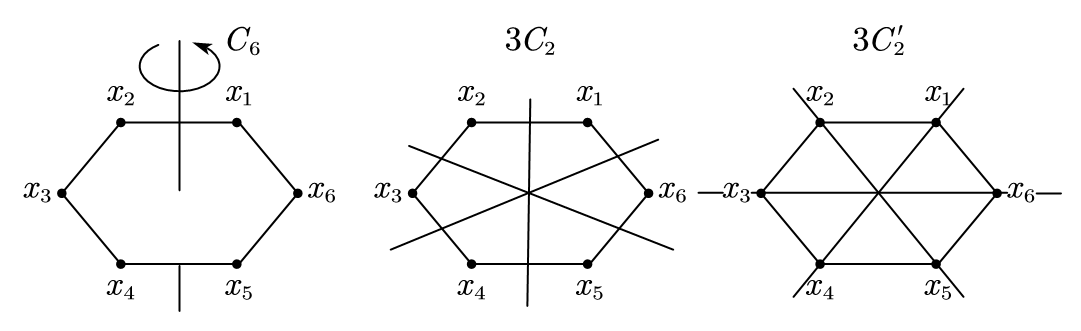
\includegraphics[width=14cm]{image/6-3-11.png}
\caption{6原子环对称性}
\end{figure}

第二种是以六边形对边连线中点构成的二重轴.\,绕它们转$180^\circ$后体系才会复原,\,典型的代表性元素:
\[C_2:\quad x_1\leftrightarrow -x_2,\,x_3\leftrightarrow -x_6,\,x_4\leftrightarrow -x_5\]

第三种是六边形的对角线作为二重轴.\,典型的代表元素:
\[C_2':\quad x_1\leftrightarrow -x_5,\,x_2\leftrightarrow -x_4,\,x_3\leftrightarrow -x_3,\,x_6\leftrightarrow -x_6\]

对称性永远都是指在某一种变换下,\,体系的某一些量具有不变的特性.\,那么我们发现,\,体系的能量函数就具有这样的特性.\,以上无论哪一个变换,\,在交换了各个$x$的角标以后,\,能量函数的表达式却恰好回到原来的表达式.\,但是对于一些不属于这个体系的对称性操作,\,比如单个$x_1\leftrightarrow x_2$.\,能量的表达式就变了.\,所以我们说体系的能量函数具有对称性.

但是体系的形状是不会具有对称性的.\,之前的示意图完全是静止状态下的苯分子\footnote{基态体系的对称性会完全等于能量函数的对称性,\,这一点也是可以被证明的.}.\,但是我们现在就是要考虑它的振动.\,作为能量函数的结果,\,其振动解是否一定具有对称的形式?\,答案显然是否定的,\,因为体系的运动由动力学方程和初始条件来决定.\,即使动力学方程是对称的,\,只要其初始条件具有不对称性,\,其解就至少有一些时刻不再对称.\,这就是说,\,\emph{对称性的原因不一定产生对称的结果}.\,这种现象就是一种广义上的\emph{对称性破缺}(symmetry breaking)现象.

但是,\,我们指出:\,如果把对称性操作理解为\emph{算符}(operator),\,它作用在一组现成的解上可以得到一种不同的运动.\,例如典型的$C_6$对称性操作,\,它把每一个原子的运动状态转移到了它的下一个原子上.\,那么我们就可以找到体系\emph{演化规律和某个对称性算符的共同本征模式}.\,这就是说,\,存在一些振动模式,\,它即是某个本征频率$\omega$下的模式,\,又恰好在某个对称性操作下(例如$C_6$)产生的运动和原来仅仅相差一个常数,\,这个常数称作\emph{本征值}(eigenvalue):
\[C_[x_i]\}=\lambda[x_i]\]

原因是简单的:\,首先如果找到了体系的一个$\omega$下的本征模式,\,那么直接用这个对称性作用在这个模式下任意次,\,显然得到的新的运动全都是原来的动力学方程的解,\,就连频率也不会改变,\,它们就全都是对应到同一个本征频率下的本征模式,\,称作\emph{简并}(degenerate)在一个频率上的模式.\,那么可以考虑得到的所有模式的组合,\,由于对称性操作连续作用有限次以后必然回到初始状态.\,故模式数必然有限.\,这样就一定可以找到合适的状态.

\newpage
例如,\,对于$C_6$,\,初始状态如果是$[x_i]_1$,\,那么至多连续作用$C_6$五次,\,第六次就回到初始状态了:
\[[x_i]_2=C_6[x_i]_1,\,[x_i]_3=C_6^2[x_i]_1,\,[x_i]_4=C_6^3[x_i]_1,\,[x_i]_5=C_6^4[x_i]_1,\,[x_i]_6=C_6^5[x_i]_1\]
\[[x_i]_1=C_6^6[x_i]_1\]

这样我们就可以构造出以下的\emph{共同本征函数}:
\[
\begin{array}{rcl}
[x_i]_{(0)}=[x_i]_1+[x_i]_2+\cdots+[x_i]_6 & \Rightarrow & C_6[x_i]_{(0)}=1\cdot[x_i]_{(0)}\\

[x_i]_{(1)}=[x_i]_1\cdot (w^1)^1+[x_i]_2\cdot (w^1)^2+\cdots+[x_i]_6\cdot (w^1)^6 & \Rightarrow & C_6[x_i]_{(1)}=w^{-1}\cdot[x_i]_{(1)}\\

[x_i]_{(2)}=[x_i]_1\cdot (w^2)^1+[x_i]_2\cdot (w^2)^2+\cdots+[x_i]_6\cdot (w^2)^6 & \Rightarrow & C_6[x_i]_{(2)}=w^{-2}\cdot[x_i]_{(2)}\\

&\cdots& \\ 

[x_i]_{(5)}=[x_i]_1\cdot (w^5)^1+[x_i]_2\cdot (w^5)^2+\cdots+[x_i]_6\cdot (w^5)^6 & \Rightarrow & C_6[x_i]_{(5)}=w^{-5}\cdot[x_i]_{(5)}
\end{array}
\]

而$w^6=1,\,w=\ue^{\ui\pi/3}$是六次单位根.\,把某个本征频率下的所有本征模式拿出来,\,对应的$C_6$算符的本征值也只有可能在以上六种值:\,六次单位根的若干幂次中选取.

同理,\,如果考虑$C_2$或者$C_2'$对称性,\,它们的本征值则更少,\,作为二次单位根仅仅只有$1$或$-1$两种可能性.\,

接下来我们可以先分析\emph{单态}(singlet).\,假设某一个角频率下仅仅只有一重简并,\,即只有一个本征模式.\,那么这个模式自己就必须同时成为$C_6,\,C_2,\,C_2'$三者的本征态.\,对于后两者有四种可能性:
\[C_2[x_i]=\pm [x_i]\quad ,\quad C_2'[x_i]=\pm [x_i]\]
\[\Rightarrow\quad \begin{bmatrix}-x_2\\-x_1\\-x_6\\-x_5\\-x_4\\-x_3\end{bmatrix} =\pm \begin{bmatrix}x_1\\x_2\\x_3\\x_4\\x_5\\x_6\end{bmatrix}\quad,\quad \begin{bmatrix}-x_5\\-x_4\\-x_3\\-x_2\\-x_1\\-x_6\end{bmatrix} =\pm \begin{bmatrix}x_1\\x_2\\x_3\\x_4\\x_5\\x_6\end{bmatrix}\]



如果两个本征值分别是$+1$和$-1$.\,那么对应的模式为:
\[[x_1,\,x_2,\,x_3,\,x_4,\,x_5,\,x_6]=x_1[+,-,+,-,+,-]\]

这样的模式恰好也是$C_6$本征值为$+1$的模式.\,对应的运动为三个相间的原子编组,\,另外三个也编组,\,两组原子反向运动的振动模式.\,用$C_2$和$C_2'$的本征值正负来标示这种模式,\,代入原来的动力学方程,\,得到:
\[-m\omega_{+-}^2A=-2kA-kA-kA\quad\Rightarrow\quad \omega_{+-}=\sqrt{\frac{4k}{m}}\]

再来考虑两个本征值都是$-1$的情况,\,这样恰好有:
\[[x_1,\,x_2,\,x_3,\,x_4,\,x_5,\,x_6]=x_1[+,+,+,+,+,+]\]

也就是所有原子都沿相同方向作相同运动.\,对应$C_6$本征值为$+1$.\,显然这样的运动就是整体作匀速旋转的运动:
\[\omega_{--}=0\]

但是另外两种情况略有不同.\,首先是两个本征值都是$+1$的情况.\,此时得到:
\[[x_1,\,x_2,\,x_3,\,x_4,\,x_5,\,x_6]=x_1[+,-,0,+,-,0]\]

抑或是两个本征值分别为$-1$和$+1$的状态.\,得到:
\[[x_1,\,x_2,\,x_3,\,x_4,\,x_5,\,x_6]=x_1[+,+,0,-,-,0]\]

我们发现,\,这些运动直接并不是$C_6$的本征态.\,但是这些运动有它存在的合理性.\,事实上画图就会发现这些运动都是可以符合动力学规律的:

\begin{figure}[H]
\centering
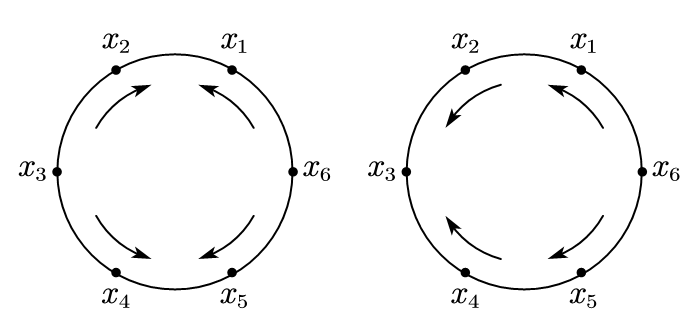
\includegraphics[width=12cm]{image/6-3-12.png}
\caption{二重简并的振动模式}
\end{figure}

每种模式的$x_1$的振动就能代表$x_1,\,x_2,\,x_4,\,x_5$四个质点的振动.\,而$x_3,\,x_6$在这两种模式下都是静止的.\,对于第一种模式,\,对$x_1$列牛顿定律:
\[-m\omega_{++}^2A=-2kA-kA\quad\Rightarrow \quad \omega_{++}=\sqrt{\frac{3k}{m}}\]
\[-m\omega_{-+}^2A=-2kA+kA\quad\Rightarrow \quad \omega_{-+}=\sqrt{\frac{k}{m}}\]

正因为这些运动合理,\,但又不是$C_6$的本征态,\,所以其实它们根本就不像最初假设的那样,\,是两个本征频率$\omega_{++},\,\omega_{-+}$下的单态,\,而是各存在二重简并.\,显然我们把$C_6$作用在这两个态上各一次就是与它简并在同一个频率上的另一个独立振动模式,\,如果设$x_1=A\ue^{\ui\omega t}$:
\[[x_i]_{++}=[+,-,0,+,-,0]A\ue^{\ui\omega_{++} t}\quad\Rightarrow\quad C_6[x_i]_{++}=[0,+,-,0,+,-]A\ue^{\ui\omega_{++} t}\]
\[[x_i]_{-+}=[+,+,0,-,-,0]A\ue^{\ui\omega_{-+} t}\quad\Rightarrow\quad C_6[x_i]_{-+}=[0,+,+,0,-,-]A\ue^{\ui\omega_{-+} t}\]

恰好,\,作用两次是徒劳的.\,两次旋转以后的运动可以用前两次的运动组合形成:
\[C_6^2[x_i]_{++}=-[x_i]_{++}-C_6[x_i]_{++}\quad:\quad [-,0,+,-,0,+]=-[+,-,0,+,-,0]-[0,+,-,0,+,-]\]
\[C_6^2[x_i]_{-+}=-[x_i]_{-+}-C_6[x_i]_{-+}\quad:\quad [-,0,+,+,0,-]=-[+,+,0,-,-,0]-[0,+,+,0,-,-]\]

从而我们就完整地找到了体系的六个本征模式:
\[\omega_{--}=0\quad:\quad [x_i]_{--}=[+,+,+,+,+,+]vt\]
\[\omega_{-+}=\sqrt{\frac{k}{m}}\quad:\quad [x_i]_{-+}=[+,+,0,-,-,0]A\ue^{\ui\omega_{-+} t}\quad,\quad C_6[x_i]_{-+}=[0,+,+,0,-,-]A\ue^{\ui\omega_{-+} t}\]
\[\omega_{++}=\sqrt{\frac{3k}{m}}\quad:\quad [x_i]_{++}=[+,-,0,+,-,0]A\ue^{\ui\omega_{++} t}\quad,\quad C_6[x_i]_{++}=[0,+,-,0,+,-]A\ue^{\ui\omega_{++} t}\]
\[\omega_{+-}=\sqrt{\frac{4k}{m}}\quad:\quad [x_i]_{+-}=[+,-,+,-,+,-]A\ue^{\ui\omega_{+-} t}\]

事实上我们只看到了问题的一个局部.\,关于复杂体系小振动背后的对称性分析是一个内容非常丰富的专题.\,它涉及到关于对称性的\emph{群论}(group theory)和对于振动在对称性操作下演化的\emph{群表示论}(group representation theory).\,它在原子分子物理,\,固体物理,\,乃至粒子物理中都有着非常广泛的应用.

对于苯分子的振动模式我们也做了过多的简化,\,下面的表是较完整地考虑碳原子和氢原子间共$12$个原子,\,在三维空间中各做三自由度运动而形成的共$36-6=30$个振动模式.\,减$6$是因为有$6$个自由度是整体的平动和转动而不是振动.\,根据对称性,\,一共有$20$种振动模式.\,其中有$10$种为二重简并.\,分子的振动光谱一般在红外线波段:
\begin{figure}[H]
\centering
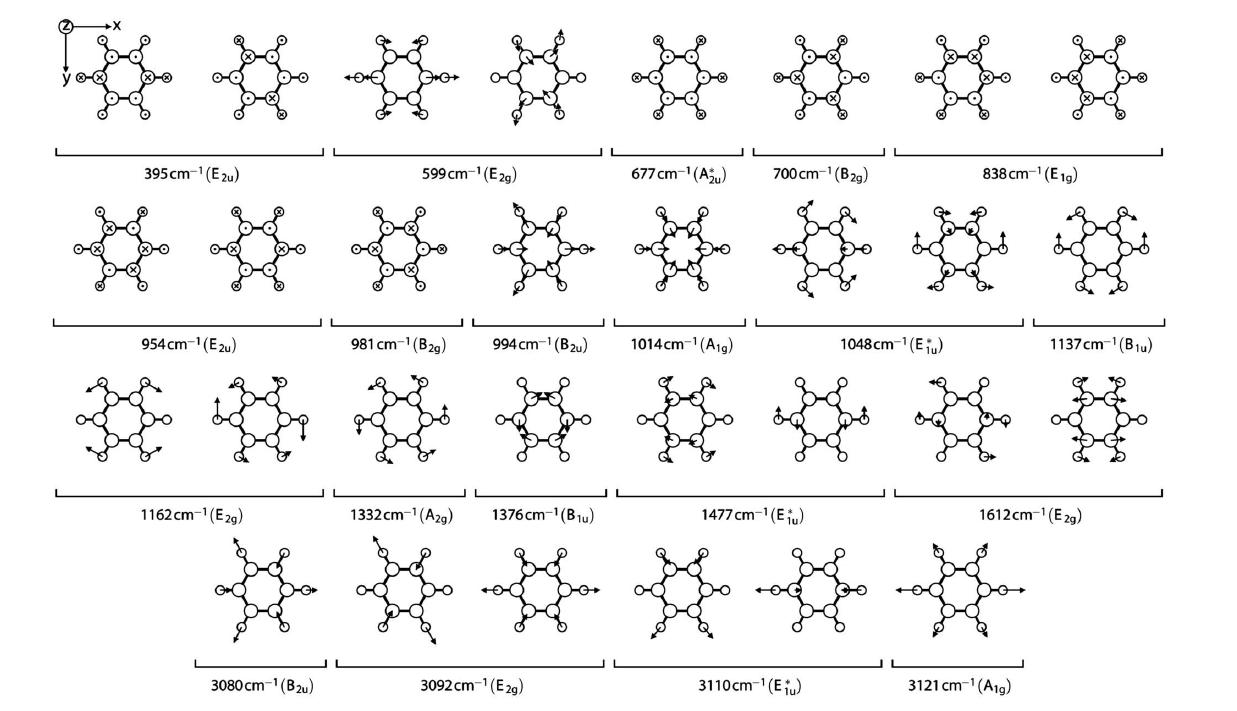
\includegraphics[width=17cm]{image/6-3-9.png}
\caption{苯分子的完整振动模式}
\end{figure}

利用原子间作用力的经验函数就可以得到各个本征角频率$\omega$.\,而由量子力学中的原理,\,振动的能量实际上是量子化的:
\[E_n=\left(n+\frac{1}{2}\right)\hbar\omega\]
苯分子的吸收光谱和发射光谱中对于相邻两个能级能量差的光子就会有共振吸收的现象:
\[\Delta E=h\nu =\hbar \omega\]

可见其实就是当电磁波的频率恰好与振动频率吻合时发生共振吸收:
\[\nu=\frac{\omega}{2\pi}\]
\newpage


\section{非线性摄动*}



\section{格波}

让我们考虑两个十分经典的\emph{固体物体}(solid state physics)问题:\,声音的本质是什么?\,固体热运动的本质是什么?\,我们可能会得到一个惊人的答案:\,两者的本质,\,都是晶格的振动.

固体,\,一般是晶体,\,它的描述方法,\,也需要照顾到电子的行为,\,也需要照顾余下的原子实---它占据着主要的质量与动能---的运动形式.\,如果把目光仅仅放在原子实上,\,认为原子实是在格点的平衡位置附近做小振动.\,而这个运动的动力学成因,\,必然是来自于初始条件和原子之间可以类比为弹簧的线性作用力.\,这样去思考问题的话,\,也许具体的计算还是困难的,\,但至少我们会有以下三个结论:

一:\,这个运动一定是牵一发而动全身的.\,一个原子的振动会带动其它原子的振动,\,一个地方的振动会带动另一个地方的振动,\,这其实就是固体可以传热和传声的原理.\,而且不出意外的,\,一般传热性能越好的固体,\,声速也就越快.\,天然材料中金刚石就是在两个方面都具有卓越性能的典型:\,它的声速高达$12000{\rm m/s}$,\,在元素单质方面仅仅次于在自然界不以单质形式存在的金属铍($13000{\rm m/s}$),\,是铁的两倍多.\,而热导率则是达到了惊人的$2000{\rm W/m\cdot K}$,\,为金属中导热性能优异的银的约五倍.

二:\,有规则的这种运动形成了声波.\,也就是宏观问题中看似连续的声波,\,在微观看来其实就是一个个分立的原子在因为弹性力而做多自由度的小振动,\,而不再具有连续性.\,这种运动就叫做\emph{格波}(lattice wave).

三:\,无限不规则的声波进行叠加就形成了热运动.\,基于这一点,\,我们其实不应该把热运动分解为每一个原子各做一个独立简谐振动,\,这样的统计方法是不能给出正确的关于固体的热学结果的,\,因为这些简谐振动根本就不``独立''.\,从爱因斯坦时代开始,\,把热运动分解为真正声波的叠加,\,并且对声波的能量进行量子化,\,称作\emph{声子}(phonon),\,这才真正能开始解释关于固体的热容等等初步的实验结果.

这一节我们暂时无法得出这些深刻结果的计算过程.\,但至少,\,我们可以尝试在完全经典的情况下对两个简化问题给出完整的动力学求解方法.

第一个问题就是\emph{一维原子链}(1D atomic chain)问题.\,把质量为$m$的物块和劲度系数为$k$的弹簧无限串接形成下图所示的体系.

\begin{figure}[H]
\centering
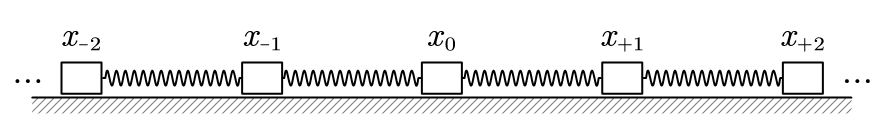
\includegraphics[width=15cm]{image/6-3-13.png}
\caption{一维原子链}
\end{figure}

这样的体系的动力学方程写作:
\[m\ddot{x}_i=-2kx_i+kx_{i+1}+kx_{i-1}\]

这样一个方程的求解其实非常类似于之前的对称性分析法.\,这里体系的对称性为平移一个单元.\,那我们就设想体系的状态为平移算符的本征态,\,即每一个物块的振动都恰好是其前一个(左边的那个,\,指标比它小一的那个)的$\lambda$倍.\,只不过这里的$\lambda$其实是一个相位因子$\ue^{\ui \varphi}$罢了.\,那么我们猜一个本征频率为$\omega$,\,在平移算符下本征值为$\lambda$的解,\,显然$\omega$就会是$\lambda$的函数:
\[x_i=\lambda^i A\ue^{\ui\omega t}\]

代入原方程,\,命$\omega_0=\sqrt{k/m}$就可以得到:
\[\frac{\lambda+\lambda^{-1}}{2}=1-\frac{\omega^2}{2\omega_0^2}\]

若$\lambda$为实数,\,不管是$|\lambda|>1$还是$|\lambda|<1$都不是我们希望得到的结果,\,这样在$i\to+\infty$和$i\to-\infty$两个方向一个振幅指数衰减,\,一个指数爆炸.\,那么根据因果律和能量守恒可以判断,\,指数爆炸那一侧是受到外力开始起振的那一侧,\,这个波根本就不能在原子链上传播,\,而是传着传着振幅就衰减掉了.\,此时等号左侧是一个绝对值大于$1$的实数.\,故我们发现当$\omega\geq 2\omega_0$时对应的波无法在一维原子链上传播.\,这个频率$\omega_c=2\omega_0$就叫做\emph{截止频率}(cut-off frequency).\,恰好为截止频率时,\,$\lambda=-1$,\,也就是这样的波虽然可以形成,\,但任何相邻两个原子振动方向彻底反向,\,它其实是一种``驻波'',\,原则上也没有在传播.

那么就只剩下$\omega\leq \omega_c$的波可以在一维原子链上传播.\,把$\lambda$写成$\ue^{\ui \varphi}$.\,我们得到:
\[\cos\varphi=1-\frac{\omega^2}{2\omega_0^2}\quad \Rightarrow \quad \omega=2\omega_0\left|\sin{\frac{\varphi}{2}}\right|\]

相邻两个原子的相位差应当是一个$\varphi\in (-\pi,\pi)$内的数.\,这是因为如果$A$比$B$相位大一个$\pi+\delta$,\,那么也可以解释为$A$比$B$相位小一个$\pi-\delta$.\,所以如果是截止频率的临界情况,\,我们也只能说相邻的原子反相,\,至于谁比谁大也是无从判断的,\,这是格波的特性.

对于上式我们更喜欢写为\emph{色散关系}(dispersion relation)的形式.\,就是说把自变量改为\emph{波矢}(wave vector).\,设相邻原子距离为$l$,\,那么产生的相位差$\varphi$可以由波矢来产生:
\[Kl=\varphi\quad,\quad K\in\left(-\frac{\pi}{l},\,\frac{\pi}{l}\right)\]

\begin{wrapfigure}[13]{o}[-10pt]{6cm}
\centering
\vspace{-1.5cm}
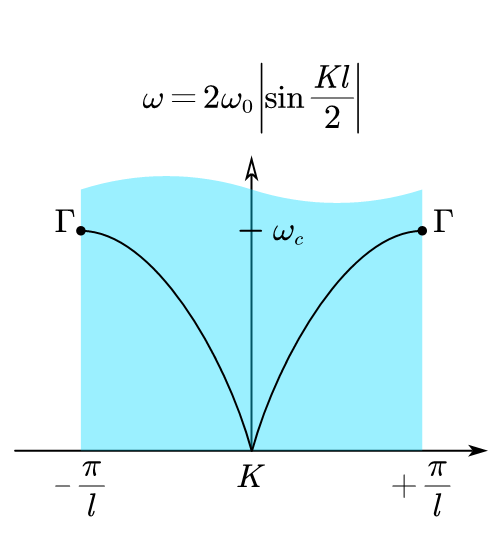
\includegraphics[width=6cm]{image/6-3-14.png}
\caption{色散关系}\label{6-3-14}
\end{wrapfigure}
上面这个$K$应当处于的空间称作\emph{布里渊区}(Brillouin zone).\,它告诉我们,\,在一维原子链上传播的格波在频率和波矢上都是受限的.\,其函数图像和表达式如图\ref{6-3-14}.

色散曲线上每一个点都代表一种能够在一维原子链上传播的振动模式:
\[x_i=A\ue^{\ui(\omega t+iKl)}\]

此时两个极限是值得关注的:

一是,\,在短波极限:\,波长最短就是当$Kl=\pi$时,\,此时波长$\Lambda=2\pi/K=2l$时,\,向左和向右延伸的色散曲线到达最高点$\Gamma$.\,但尤其要注意两个$\Gamma$点实质上就是同一个点,\,对应完全相同的状态.\,可以想想把第一布里渊区卷做一个圆柱,\,让两个$\Gamma$点重合.\,对应的相邻原子彼此反相的``驻波''形式.\,也就是说如果让$K>0$的右行波的$K$持续增加以跨越$\Gamma$点,\,波就演化为左行波了.\,个中缘由在于$K$的正负指称的速度其实是\emph{相速度}(phase velocity),\,但在判断波的传播方向时,\,其实\emph{群速度}(group velocity)才是更加合理的选择.\,它被定义为:
\[v_g=\frac{\ud \omega}{\ud K}\]

其中的原理我们将在流体的相关波动章节中简介.

二是,\,在长波极限:\,$\Lambda\gg l$.\,此时$Kl$时一个小量,\,可以对$\sin$使用近似,\,物理上代表相邻两个原子几乎是以相同的方式运动,\,微观波变成了宏观的波:
\[\omega=\omega_0Kl\]

这就给出了波的传播速度:
\[v=\frac{\omega}{K}=\omega_0 l=\sqrt{\frac{k}{m}}l\]

这个结果与宏观波速公式$v=\sqrt{E/\rho}$是完全一致的.\,且看之后弹性体章节的分析.

\vspace{1cm}

最后我们还看看\emph{双原子链}(diatomic chain)与以上\emph{单原子链}(monoatomic chain)产生的并不平凡的区别.\,双原子链就意味着虽然其平移周期还是$l$,\,但每一个单元内部出现了两个待求解的坐标.\,我们让两个原子质量分别为$M,\,m$,\,弹簧劲度系数依然为$k$:
\begin{figure}[H]
\centering
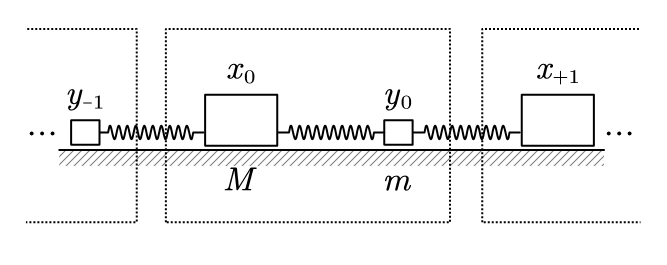
\includegraphics[width=10cm]{image/6-3-15.png}
\caption{双原子链}
\end{figure}

那么对应的动力学方程写作:
\[M\ddot{x}_i=-2kx_i+ky_i+ky_{i-1}\]
\[m\ddot{y}_i=-2ky_i+kx_i+kx_{i+1}\]

由于有单原子链的经验.\,我们让$\omega_0=\sqrt{k/2M}$\footnote{即先忽视$m$的存在让弹簧直接串联.},\,而$m=\beta M$.\,并直接设解为:
\[x_i=A\ue^{\ui(\omega t+iKl)}\quad,\quad y_i=B\ue^{\ui(\omega t+iKl)}\]\

其中$A$和$B$是复振幅可以差一个相位.\,那么这就给出:
\[
\begin{array}{rcrc}
(4\omega_0^2-\omega^2)A&+&-2\omega_0^2(1+\ue^{-\ui Kl})B&=0\\
-2\omega_0^2(1+\ue^{\ui Kl})A&+&(4\omega_0^2-\beta\omega^2)B&=0
\end{array}
\]

这个方程组$A,\,B$的解不为零的条件就是:
\[(4\omega_0^2-\omega^2)(4\omega_0^2-\beta\omega^2)=4\omega_0^4(1+\ue^{\ui Kl})(1+\ue^{-\ui Kl})=16\omega_0^4\cos^2\frac{Kl}{2}\]

在$\beta$是个小量的情况下,\,我们可以近似地求解这个方程.\,在任意$K$下这个方程与单原子链不同,\,它$\omega^2$总是有两个解.\,第一个解发生在$\omega$与$\omega_0$量级相当的情况下,\,此时$4\omega_0^2-\beta\omega^2\approx 4\omega_0^2$.\,近似可以得到:
\[\omega=2\omega_0\left|\sin{\frac{Kl}{2}}\right|\]

可以发现这个解与只含$M$的单原子链的结果并没有什么区别.\,所以其实是这种模式下,\,主要的动力学效果由$M$承担,\,$m$则几乎平衡在两侧的$M$中间.\,两个相邻的$M$之间的两段弹簧几乎就是直接串联在一起,\,同时伸长同时缩短,\,感受不到很轻的$m$的影响.

而另外一个解则发生在$\omega\gg \omega_0$的极端情况下,\,此时$4\omega_0^2-\omega^2$本是一个绝对值很大的负数,\,它$\approx -\omega^2$.\,但是与另一个因子$4\omega_0^2-\beta\omega^2$相乘时又回到正的$\omega_0^4$量级的等式右侧了.\,从而乘的因子其实很接近零:
\[4\omega_0^2-\beta\omega^2\approx 0\quad\Rightarrow \quad \omega\approx \frac{2\omega_0}{\sqrt{\beta}}\]

为了更精确地找到这个频率与$K$的函数关系,\,我们把原方程的$4\omega_0^2-\omega^2$项除到等号右边,\,并近似:
\[\omega\approx \frac{2\omega_0}{\sqrt{\beta}}\cdot\sqrt{1+\beta\cos^2\frac{Kl}{2}}\]

\begin{wrapfigure}[13]{o}[-10pt]{8cm}
\centering
\vspace{-0.5cm}
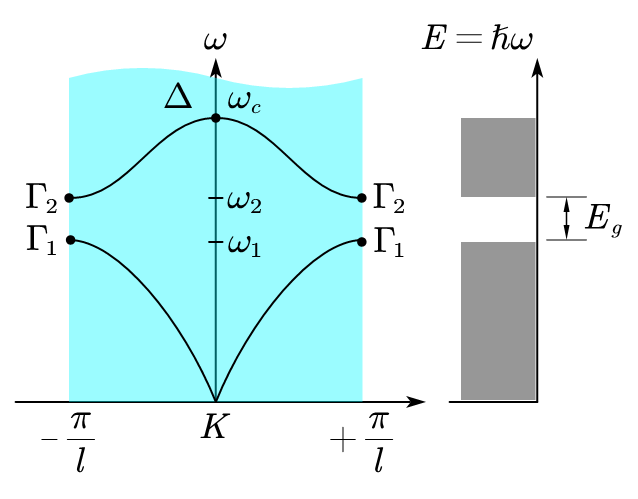
\includegraphics[width=8cm]{image/6-3-16.png}
\caption{声学支与光学支}\label{6-3-16}
\end{wrapfigure}
这样的两组解看似近似,\,但是其实在特征点处的性质和坐标又是完全准确的.\,特征点就是指波矢为零$K=0$和波矢为$\pm \pi/l$的布里渊区中心和边界上的点.\,我们把两组$\omega(K)$关系画成色散曲线如图\ref{6-3-16}.\,对应的特殊点$\Gamma_1,\,\Gamma_2,\,\Delta$对应的特殊频率为:
\[\omega_1=2\sqrt{\frac{k}{2M}}\quad ,\quad \omega_2=2\sqrt{\frac{k}{2m}}\]
\[\omega_c=2\sqrt{\frac{k}{2\mu}}\;(\mu=\frac{Mm}{M+m})\]

现在终于可以发现,\,多出来的第二组解,\,对应了在原来的色散曲线上方又多出来一支.\,这一支在$\Delta$的行为具有代表性:\,即使$K=0$,\,即相邻两个单元之间完全没有相位差.\,但是依然有很大的角频率.\,也就是这个振动并没有传播,\,而从角频率的表达式来看,\,其实就是每一个单元内部两个物体在弹性力作用下做二体小振动.\,而从$\Gamma_2$到$\Delta$点这样一段色散曲线对应的各个波动模式下,\,十分显著的一点就是轻的原子一定要主动振动起来而且与相邻的重原子根接近反相而不是同相.\,最边缘的$\Gamma_2$点则只有轻的原子在振动.\,这样的模式的频率,\,其实与上一节讨论过的分子振动频率相当,\,就在光的红外线频段,\,故把这样的一支振动模式称作色散曲线的\emph{光学支}(optical branch).

所以原来单原子链的保留支,\,特点是从$\omega=0,\,K=0$延续到布里渊区边缘的$\Gamma_1$,\,就相应的被称作\emph{声学支}(acoustic branch).\,因为在长波极限$K\to 0$下,\,这个模式的轻重原子之间是没有相位差的,\,而不是像光学支那样反相,\,这样就相当于宏观地看整个原子链在较大范围内做宏观平移.\,形成的波就是常规意义下的声波.\,在声学支模式下,\,轻的原子跟随重的原子而运动,\,相邻轻重原子更加接近同相而不是反相.\,而极限点$\Gamma_1$对应的情况是只有重原子在振动,\,轻原子全部静止了.

最后我们指出,\,简单的计算产生的结果中还蕴含着意义非凡的一个物理图像.\,那就是\emph{能带}(energy band)结构的产生.\,在这里我们着眼的是晶格上的波动,\,色散曲线上每一个点都代表一种可能的波动模式,\,其振幅,\,在经典物理中,\,由初始条件决定,\,且是可以连续变化的.\,但是量子理论预言,\,这个能量实则在低能量时量子化:
\[E_n=\left(n+\frac{1}{2}\right)\hbar\omega\]

从而色散曲线的这一副图,\,实际上也代表量子化的振动的\emph{元激发}(elementary excitation)的能量单位与$K$的关系图.\,更有甚者,\,如果我们不是去考虑晶格振动的动能加势能的元激发,\,而是去考虑在晶格间运动的电子,\,它的能量也会产生非常类似的但更复杂的能带结构\footnote{会往上产生更多能带.},\,毕竟电子在其中的描述也应当使用物质波,\,它具有波矢$K$和相应的能量$E(K)$.\,而为什么这个$E(K)$的函数也会产生类似的行为,\,这一点可以纯粹从电子满足的\emph{薛定谔方程}(Schr\"odinger equation)和对称性分析出发得到.\,在介质中的电子的波矢$K$其实也是受限的.\,而同一个$K$对应的能量也可以有多个,\,分别在不同分支的色散曲线上.\,故我们把每一条色散曲线对应的可取能量区间叫做\emph{允带}(allowed band).\,而允带之间没有对应状态的能量区间叫做\emph{禁带}(forbidden band).\,两个相邻的允带之间的禁带宽度就是\emph{带隙}(band gap).

这样一种全新的看待振动的能量,\,电子的能量的理论就是能带论.\,尤其是把电子视作物质波,\,利用量子力学完整地计算固体中的电子的运动,\,从而非常好地解释了历史上残留的金属电导率,\,热导率相关的疑问并很好地带动半导体物理学的成熟的理论,\,以它的主要缔造者:\,瑞士-美国物理学家布洛赫\,命名为\emph{布洛赫理论}(Bloch theory).

能带结构是一种介于\emph{自由电子}(free electron)和\emph{紧束缚电子}(tight-binding electron)之间的存在形式.\,在真空中的自由电子满足:
\[E=\frac{\hbar^2K^2}{2m}\]

其能量完全可以连续的改变.\,但是在束缚态上,\,如氢原子外的电子,\,简单地由玻尔模型,\,电子的能量被量子化为能级结构:
\[E=-\frac{me^4}{8n^2\varepsilon_0^2h^2}=-\frac{13.6{\rm eV}}{n^2}\]

那么在金属中的电子,\,微观上自由:\,可以脱离金属原子的束缚而传导,\,但宏观上,\,本质又是被束缚的:\,被所有原子核共同产生的吸引力束缚在金属内部.\,所以就体现出一种折衷:\,紧束缚的能级展开为能带,\,具有一定的能量连续变化的范围.\,但是能带与能带之间依然是分立的,\,没有像真空那样连成一片.


%%!TEX root = ../physical-olympics-2.tex
\chapter{万有引力}


\section{有心力下运动}

天体运动中起到核心作用的相互作用力都是\emph{有心力}(central force),\,事实上不光是天体运动,\,任意两个可以近似为质点的物体之间的相互作用力,\,根据牛顿第三定律的要求,\,其受力方向都必须沿着两个物体的连线方向.\,那么我们只要做两个要求,\,这就构成了一个有心力问题:

一是,\,这个力必须是保守力,\,即,\,它必须由势能生成:
\[V(\bs{r}_1,\,\bs{r}_2):\quad\,\bs{F}_1=-\nabla_1V\;,\,; \bs{F}_2=-\nabla_2V\]

根据我们之前的说法,\,根据对称性或牛顿第三定律,\,这个势能其实就是两个质点连线距离$R$的函数$V(R)$.\,而以$1$为中心向$2$引$\bs{R}$矢量,\,则:
\[\bs{F}_2=-V'(R)\bs{e}_{\bs{R}}=F(R)\bs{e}_{\bs{R}}\]

二是,\,中心物体$1$必须不动或者是近似不动.\, $1$不动是指有外力作用在$1$上以维持其静止.\,但$2$上不应该有这样的外力,\,而仅仅是在$1$对$2$产生的$\bs{F}_2$作用下做运动.\,$1$近似不动是比如考虑太阳系这种典型情况,\,太阳虽然受到多个行星对它的万有引力,\,但是由于自己质量过重从而近似是不动的.\,即使是地球月亮构成的二体问题,\,地球和月亮并不一定能认为都不动,\,我们也有相应的转化为有心力问题的方法,\,见后.\,最后当然,\,也有一些更简单的情况,\,$2$受到一些更复杂的体系对它的力构成了有心力$F(R)$,\,比如弹性绳对绳端质点的拉力.



\section{万有引力下运动}

\section{二体与潮汐}


%%!TEX root = ../physical-olympics-2.tex
\chapter{刚体}


\section{刚体的物理描述}
近代以前人们意识到了物质世界的\emph{连续性}(continuum),\,同时针锋相对地也提出了\emph{原子论}(atomism).\,原子最简单的模型就是质点,\,而调和物质连续性与原子学说的中间模型就是\emph{刚体}(rigid body)模型.\,刚体是不允许形变发生的系统.\,由牛顿力学对质点的讨论推广到质点系的讨论,\,使我们也很容易将相关结论进一步推广到刚体.

由于刚体上一点受力,\,则整体同时运动起来,\,这个模型与相对论力学体系是不兼容的.\,具体来说,\,相互作用必须以有限的速度传播,\,否则就违背了因果律.\,刚体不符合因果律这一时空的固有结构.\,在很多相对论情境下将招致矛盾的结果.

刚体的物理学量是哪一些呢?\,必要的内禀的属性是其质量的分布.\,某一默认时刻$t_0$刚体占据了空间区域$\Omega_0$,\,由大量体积微元$\ud V$(记做$\ud^3\bs{R}_0$)组成,\,则刚体的总质量为:
\[m=\int\limits_{\Omega_0}\rho(\bs{R}_0)\ud^3\bs{R}_0=\int\limits_{\Omega_0}\ud m\]

\begin{wrapfigure}[17]{o}[-10pt]{7cm}
\vspace{-0.4cm}
\centering
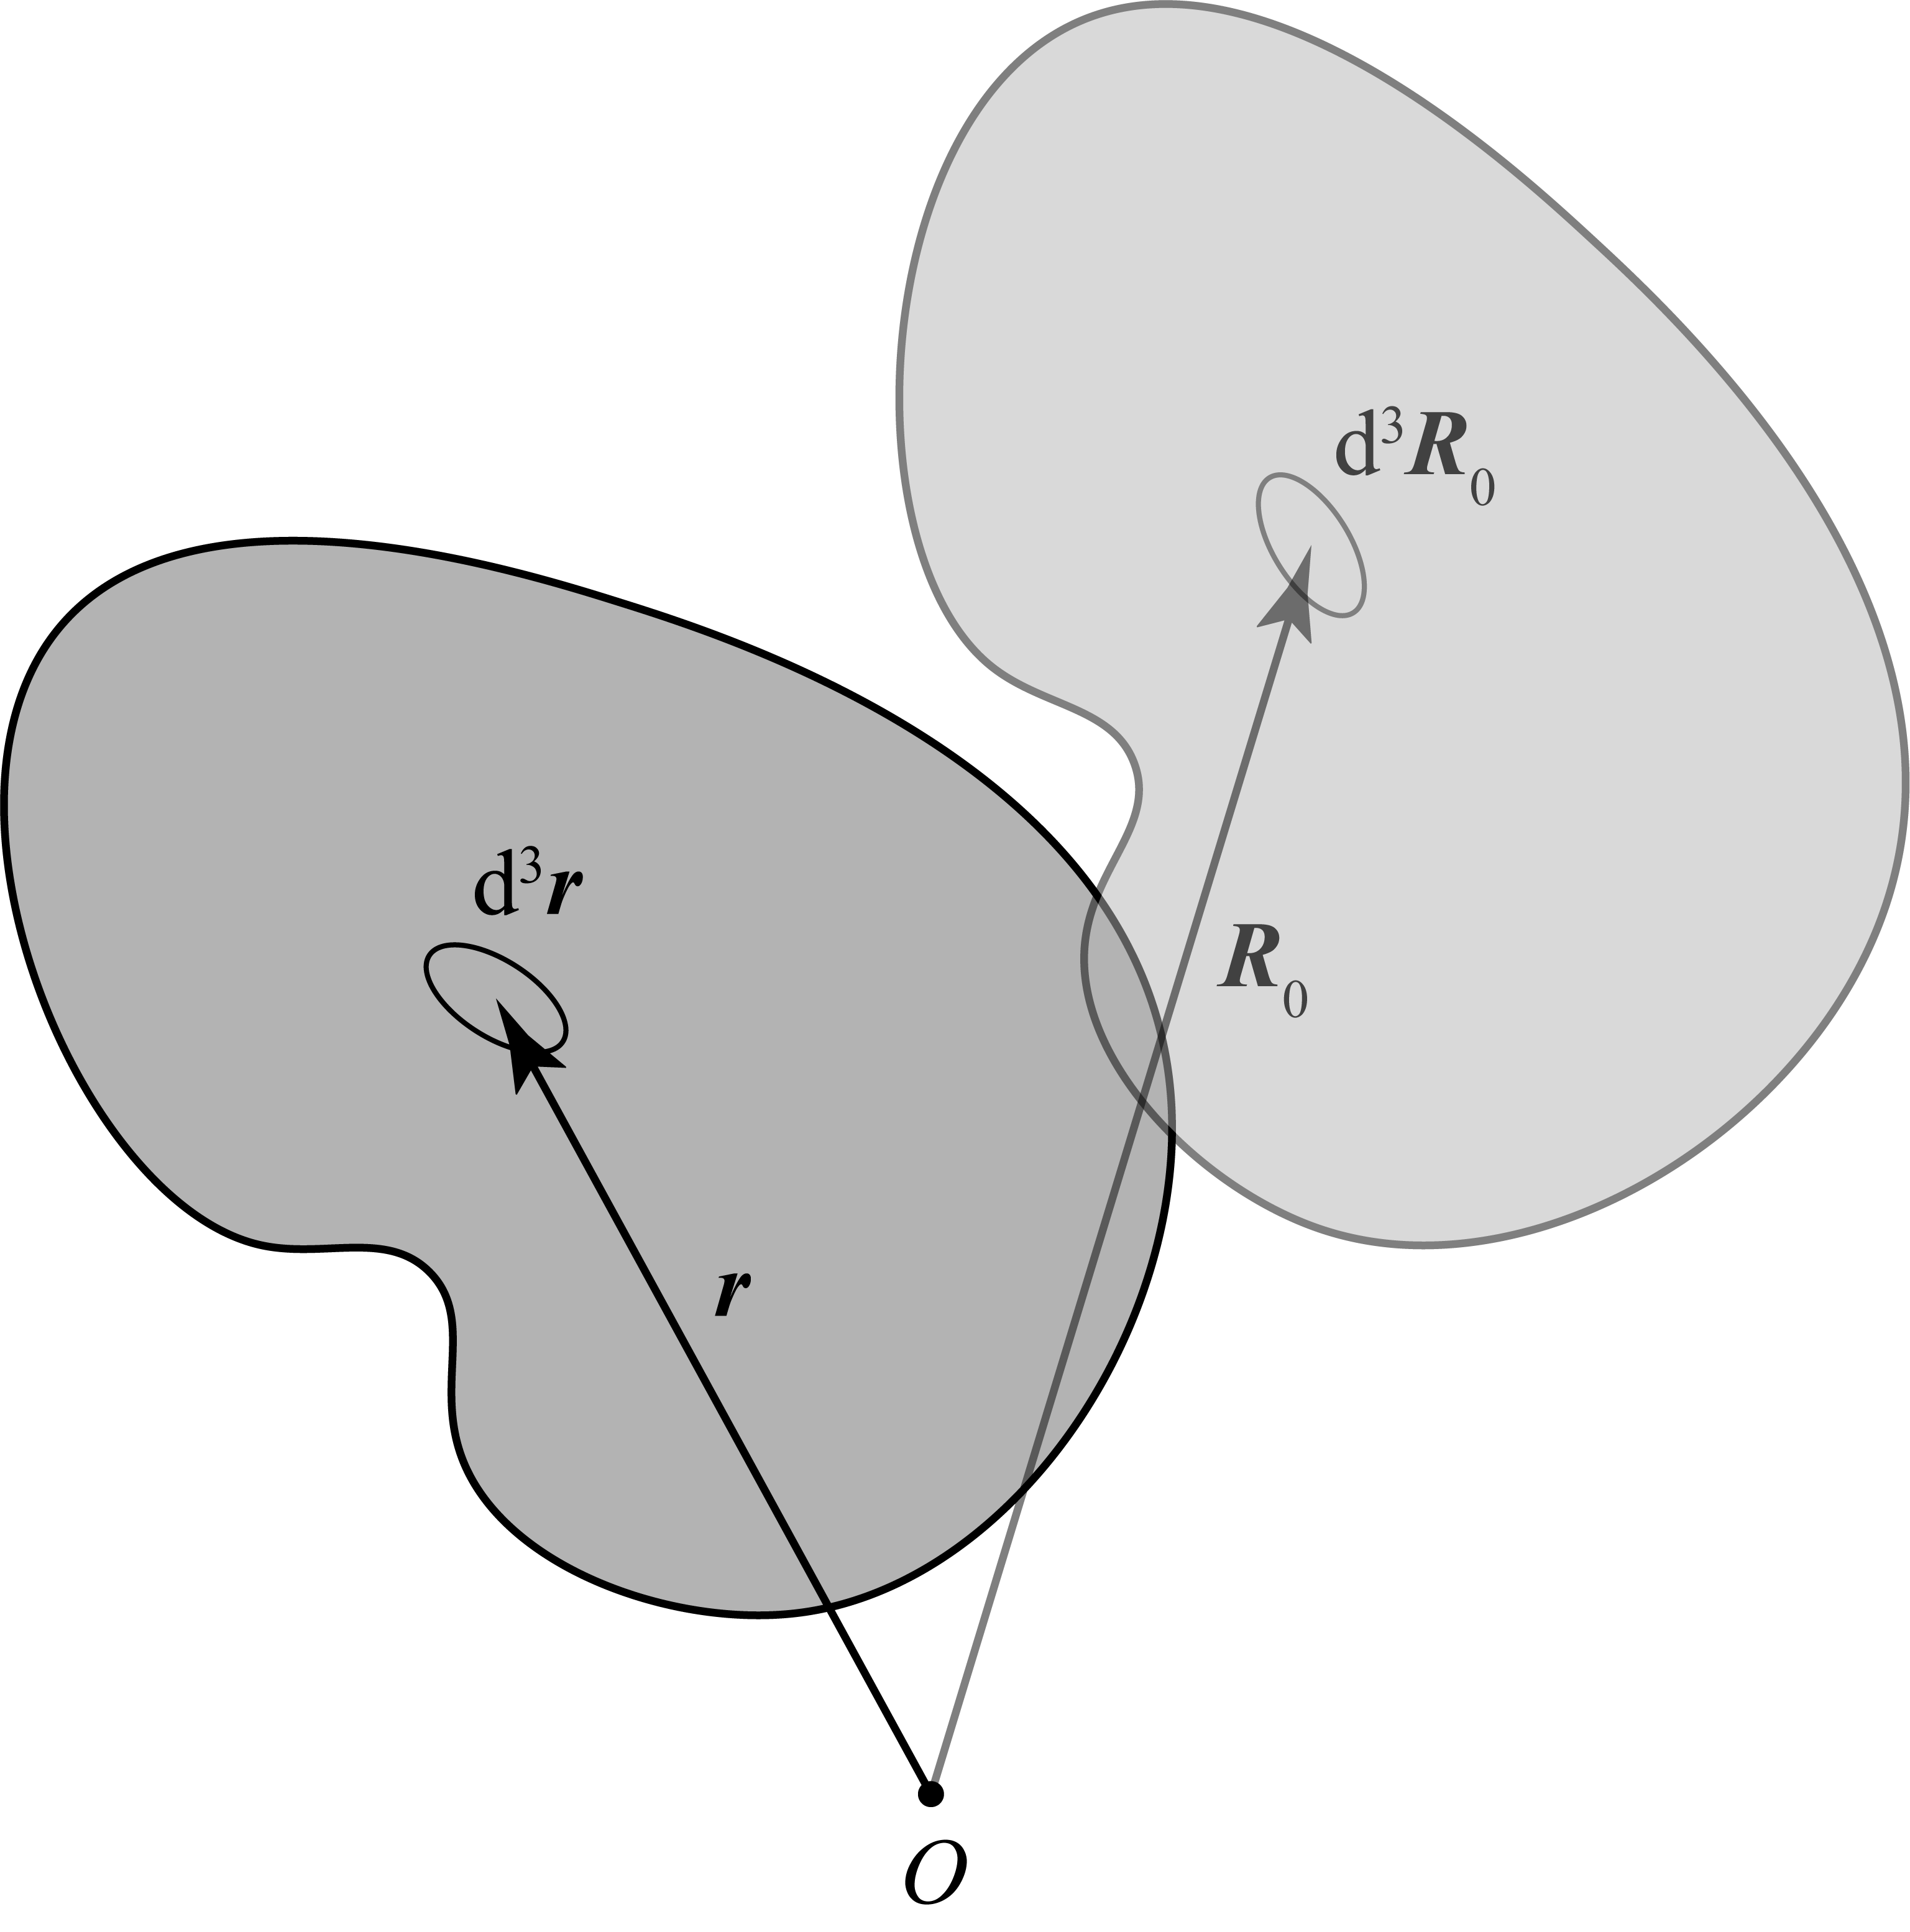
\includegraphics[width=7cm]{image/6-6-1.png}
\caption{刚体的描述}
\end{wrapfigure}
随着刚体的运动,\,原来在$\bs{R}_0$处的体积元现在在$t$时刻位于$\bs{r}$处,\,整个刚体的运动由一个多元映射来定义:
\[f:\quad \bs{R}_0,\,t\;\;\longrightarrow\;\; \bs{r}(\bs{R}_0,\,t)\]

刚体的刚性的要求,\,使得这个映射必须保持体积元的不变性:
\[f:\quad \ud^3\bs{R}_0\in\Omega_0\;\;\longrightarrow\;\; \ud^3\bs{r}\in\Omega \quad ;\quad \ud^3\bs{R}_0=\ud^3\bs{r}=\ud V\]

而且所有这个体积元内的所有内禀属性,\,这里包括密度都不能变.\,所以质量元$\ud m$也是不变的.\,从而刚体具有不变的总质量.\,马上就会发现,\,\emph{质量几何}(mass geometry)对刚体的动力学来说也十分重要.\,质量几何研究质量对特定原点$O$的各级\emph{矩}(moment).\,其中零级矩即为质量:
\[M^0=m=\int\limits_\Omega \ud m\]

一级矩是个矢量,\,它定义了刚体的\emph{质心}(center of mass)的位置:
\[M^1_i=mr_{Ci}=\int\limits_\Omega r_i\ud m\]
\[\bs{r}_C=\frac{\int\limits_\Omega \bs{r}\ud m}{\int\limits_\Omega \ud m}\]

二级矩则是一个张量,\,它的九个分量代表\emph{惯量积}(product of inertia):
\[M^2_{ij}=\int\limits_\Omega r_ir_j\ud m\]

这些矩和原点的选取有关,\,随着刚体的运动也会不断变化,\,这三阶矩的信息对刚体动力学来说就是充分的了,\,通过后面的动力学可以发现,\,刚体的运动完全依赖于外力和这三阶矩.\,如果要研究广义相对论里的引力波辐射问题,\,更高阶的矩才变得重要起来.

刚体的运动可以被我们更精确地描述,\,在$t_0$时刻建立固定在刚体上,\,沿$x,y,z$三方向的单位矢量$\bs{e}_1,\bs{e}_2,\bs{e}_3$,\,那么刚体的运动同时也把三个矢量旋转到新的三个方向:
\[f:\quad \bs{e}_i\;\longrightarrow\; \bs{\varepsilon}_i\]

这三个矢量仍然要互相垂直,\,且长度为一.\,这在数学上导致了可以通过这三个矢量的导数定义\emph{角速度}(angular velocity)矢量的结果:
\[\dot{\bs{\varepsilon}}_i=\bs{\omega}\times\bs{\varepsilon}_i\]

\begin{wrapfigure}[15]{o}[-10pt]{7cm}
\vspace{-0.7cm}
\centering
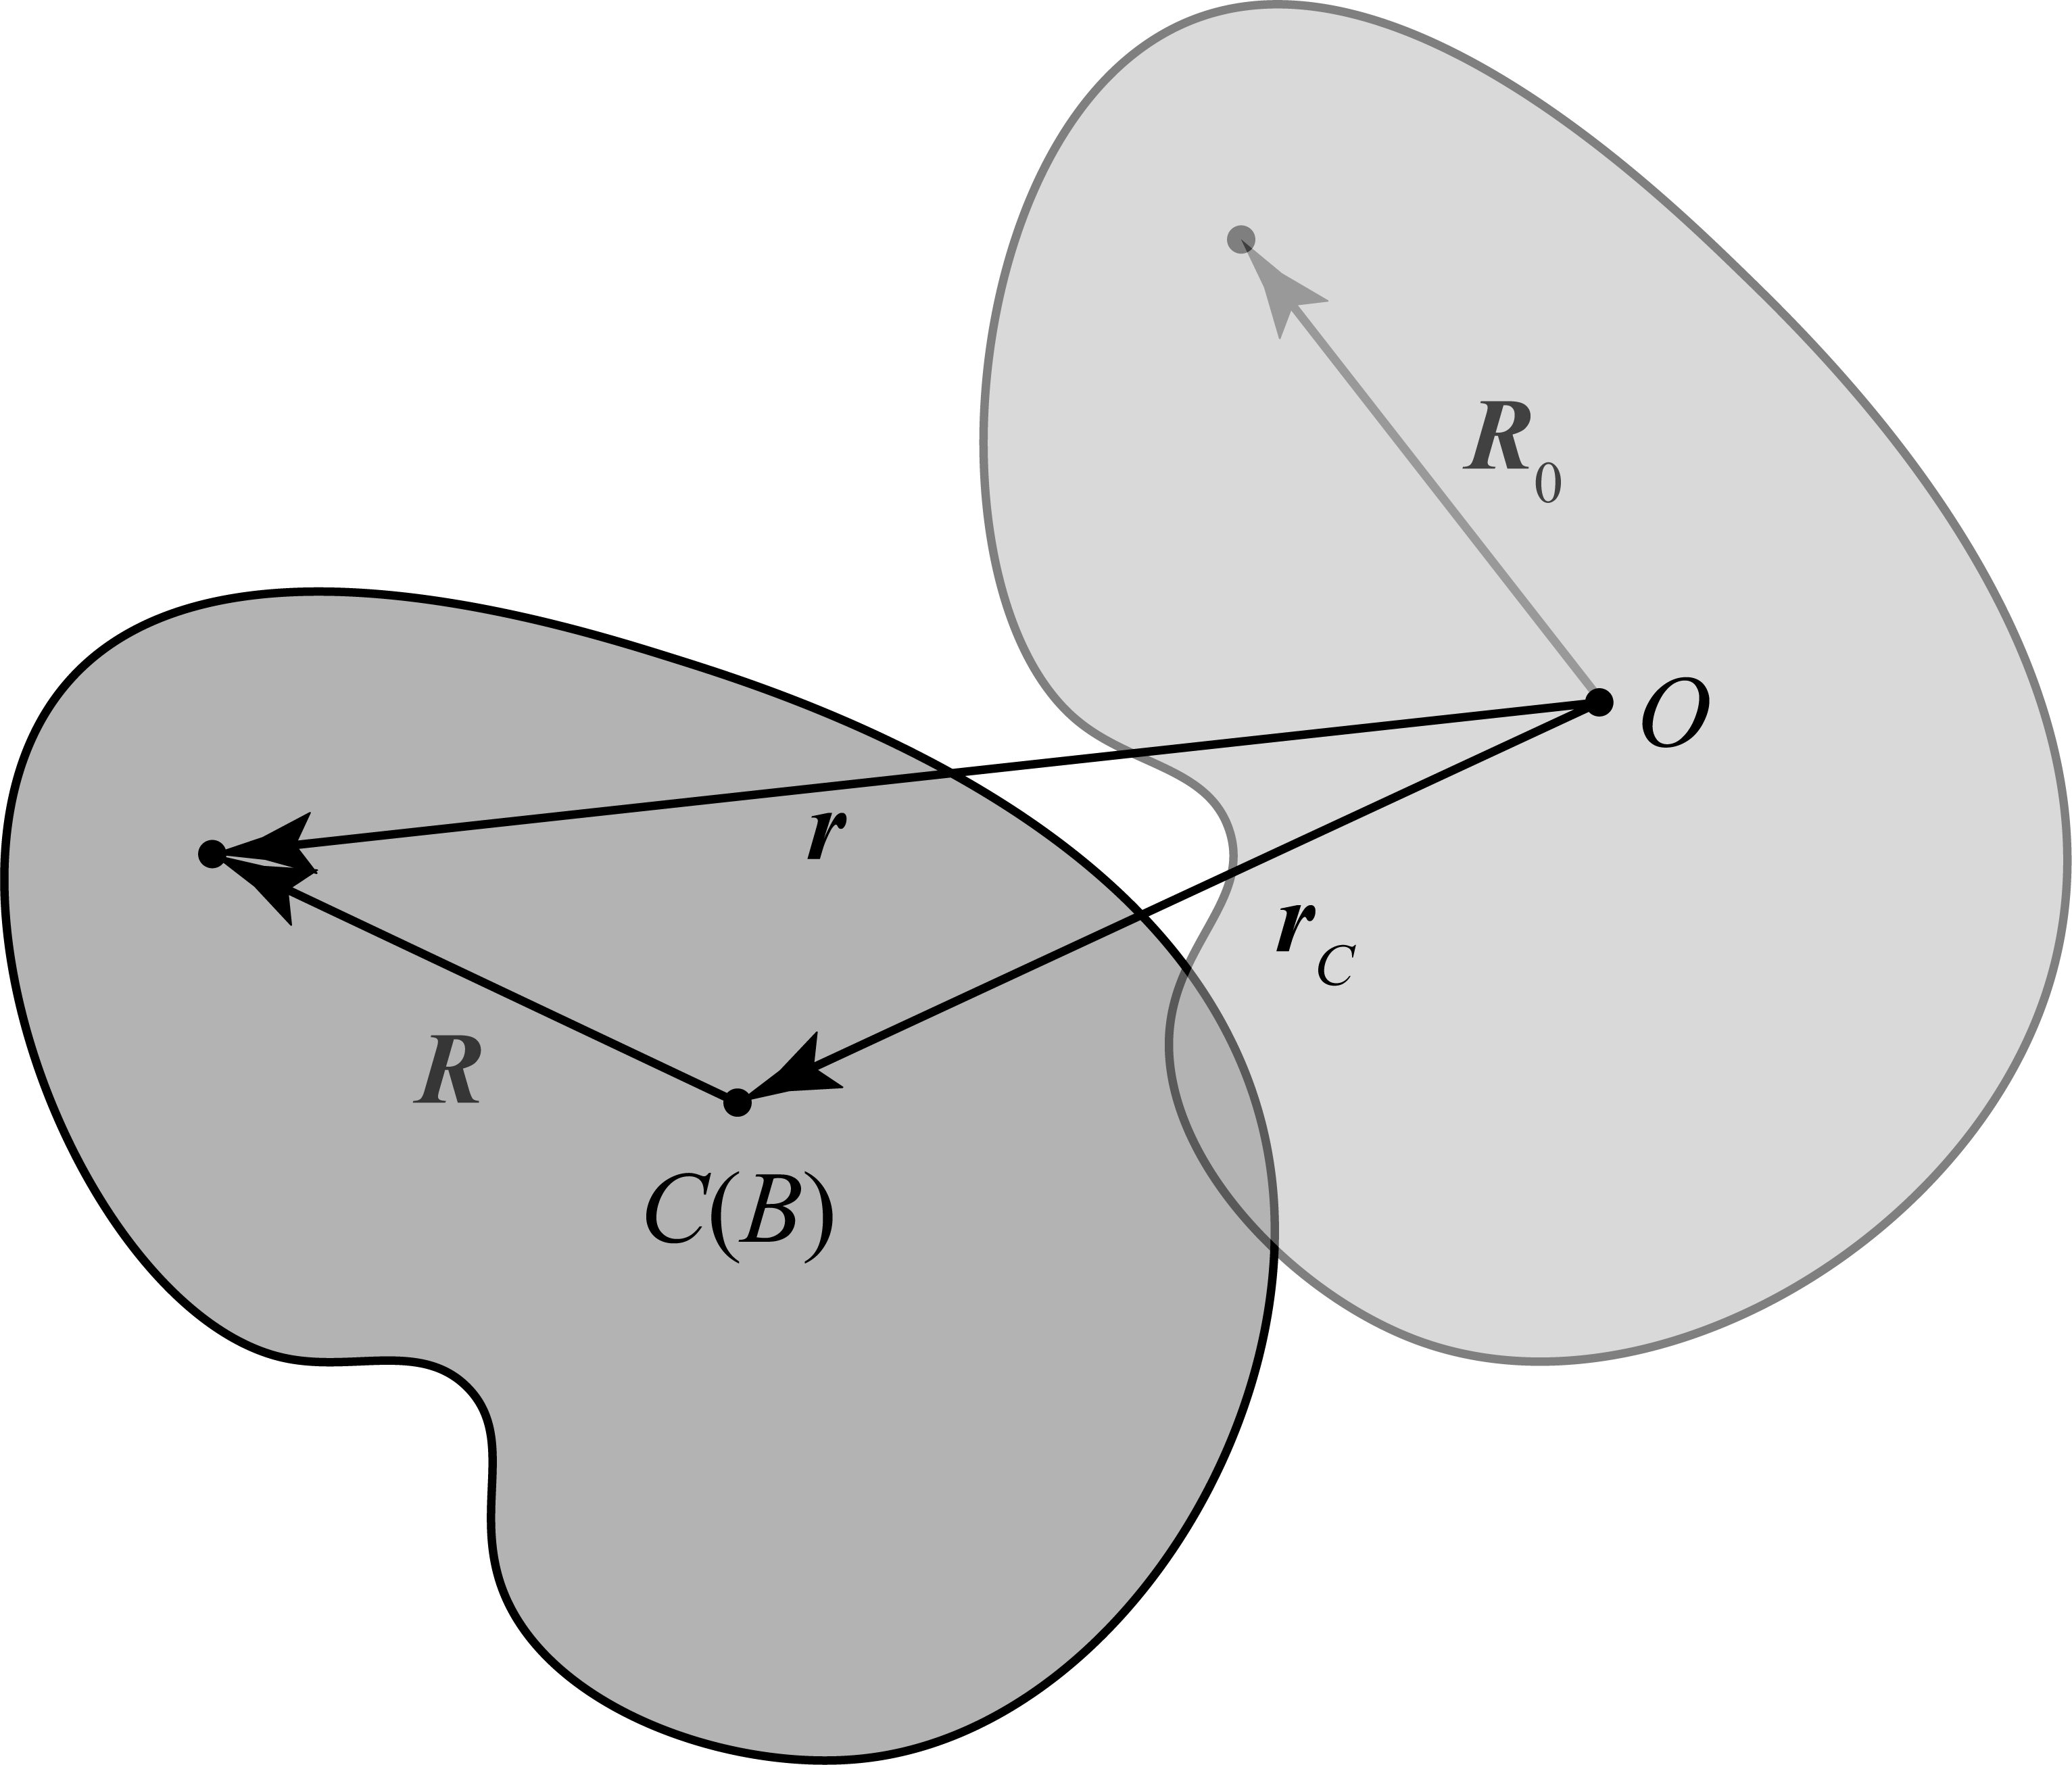
\includegraphics[width=7cm]{image/6-6-2.png}
\caption{基点法}
\end{wrapfigure}
十分类似于旋转参考系的变换的运动学,\,刚体的运动实际上就是有一个唯一的旋转参考系固连在刚体上,\,以后称作\emph{刚体系}(reference system of rigid body),\,要研究的刚体上各个点速度实际上就是刚体系中定点的运动.\,于是习惯上我们采用\emph{基点法}(method of base point)来计算刚体上任意点的运动学量.\,定义\emph{基点}(base point)为$t_0$时刻$\bs{R}_0=\bs{0}$的点$B$,\,之后的位矢为$\bs{r}_B$,\,对应的基点速度加速度为$\bs{v}_B,\,\bs{a}_B$,\,而刚提上待研究的点相对基点的位矢为$\bs{r}-\bs{r}_B=\bs{R}$,\,那么该点的速度加速度即为:
\[\bs{v}=\bs{v}_B+\bs{\omega}\times\bs{R}\]
\[\bs{a}=\bs{a}_B+\bs{\omega}\times(\bs{\omega}\times\bs{R})+\dot{\bs{\omega}}\times\bs{R}\]

出于动力学的考虑,\,基点$B$一般就取做质心$C$.\,作用在刚体上$\bs{r}$处的力$\bs{F}$固然对原点会有力矩$\bs{M}$,\,但是为了研究使刚体自身转动的效应,\,考虑到这个力同时也会使得质心运动起来,\,故我们重视这个力相对质心的力矩$\bs{M}_C$:
\[\bs{M}=\bs{r}\times\bs{F}\]
\[\bs{M}_C=\bs{R}\times\bs{F}\]

刚体受到一个力系${\bs{F}_i}$的作用,\,那么以下六个定理则来自于之前的动力学理论:
\[\sum_i\bs{F}_i=\frac{\ud \bs{p}}{\ud t}\quad ; \quad \sum_i\bs{F}_i=m\bs{a}_C\]
\[\sum_i \bs{v}_i\cdot \bs{F}_i=\frac{\ud }{\ud t}(\frac{1}{2}m\bs{v}_C^2+E_{kr})\quad ;\quad \sum_i(\bs{v}_i-\bs{v}_C)\cdot \bs{F}_i=\frac{\ud E_{kr}}{\ud t}\]
\[\sum_i \bs{r}_i\times \bs{F}_i=\frac{\ud }{\ud t}(\bs{r}_C\times m\bs{v}_C+\bs{L}_r)\quad ;\quad \sum_i \bs{R}_i\times \bs{F}_i=\frac{\ud \bs{L}_r}{\ud t}\]

前两个式子实际上几乎没有区别,\,因为刚体的总动量其实就是质心动量$\bs{p}=m\bs{v}_C$.\,后面几个式子则涉及到相对(平动)质心系的能量与角动量.\,它们与质量二级矩有着密切的联系,\,我们在第三讲\ref{6.3}阐明.\,现在我们写出相对质心系能量角动量的定义:
\[E_{kr}=\int\limits_\Omega \frac{1}{2}(\bs{\omega}\times \bs{R})^2\ud m\]
\[\bs{L}_r=\int\limits_\Omega \bs{R}\times(\bs{\omega}\times \bs{R})\ud m\]




\section{平面平行运动}
一个底面磨平的物体贴在平坦的地面上运动给人以\emph{平面平行运动}(plane-parallel motion)的概念.\,其他的一些物体运动特征也相似于它:\,黑板刷在黑板上的运动,\,车轮在直行时的滚动...\,它们的特征是:\,刚体任何一个体积元都在一个特定的平面上运动,\,而这些平面又彼此平行.\,对于这样的运动基点法只需要给出质心$C$的位矢$\bs{r}_C$和对$t_0$时刻刚体转过的角度$\theta$即可.\,角速度与角加速度即可用角度的导数来给出$\omega=\dot{\theta},\,\beta=\ddot{\theta}$.\,一般来说,\,在垂直于这些平面方向要么由于动力学对称性不需要也不存在任何作用力.\,要么这些力作为约束平面对物体的约束力而不在我们考虑范围内.\,所以我们对一些物理对象做如下修改:\,
\begin{itemize}
\item 所有参考点改成垂直平面过该点的参考轴.\,并约定其正方向
\end{itemize}
\section{空间刚体运动*}\label{6.3}



%%!TEX root = ../physical-olympics-2.tex
\chapter{流体}



\section{流体的物理描述}

\section{定常流动动力学}

\section{黏滞流体动力学}

\section{流体中的波}

\section{波的色散}
%%!TEX root = ../physical-olympics-2.tex
\chapter{弹性体}


\section{弹性体的物理描述}

所谓弹性体就是完全\emph{弹性}(elasticity)的物体.\,弹性描述的是使物体发生形变的力撤除以后物体可以回到静息状态的属性.\,弹性力学研究的对象与范围就是弹性体的力学性质.\,一般来说,\,固体主要具有弹性而液体主要具有黏性,\,若是研究中间的状态,\,\emph{非牛顿流体}(non-newtonian fluid)和\emph{塑性固体}(plastic solid),\,那就是\emph{黏弹性力学}(rheology)要研究的对象了.\,典型的黏弹性过程受力不是简单地正比于位移而是与速度,\,与历史相关.\,因此而可以发生永久的不可恢复的变形.

正因为如此,\,完整描述弹性体的运动学时,\,不得不额外留心所有点的实际位移.\,在流体时也许速度更需要注意.\,所以我们写出一个初始$t=0$位置矢量为$\bs{R}$的点,\,经过$t$时间到达位置为$\bs{r}$处,\,也就是我们要定义一个$\mathrm{3D}\times\mathrm{1D}$到$\mathrm{3D}$的映射:
\[\bs{r}=\bs{r}(\bs{R},t)\]

不失普遍性地,\,我们考虑如何刻画在$\bs{R}=\bs{0}$的形变.\,我们需要研究在$\bs{R}=\bs{0}$的附近$\ud \bs{R}=\ud X\bs{e}_x+\ud Y\bs{e}_y+\ud Z\bs{e}_z$处的位移$\bs{\delta}=\bs{r}-\bs{R}$与中心的位移去比较.\,数学上有以下泰勒展式:
\[\bs{\delta}(\ud \bs{R},t)=\bs{\delta}(\bs{0},t)+\ud \bs{R}\cdot \nabla \bs{\delta}\]

上式中$\nabla\bs{\delta}$是一个有九个分量的张量,\,张量这一概念上一章介绍过,\,它是九个分量的三行三列式的组合,\,现在它的作用是可以与之前的矢量$\ud \bs{R}$点乘把它线性地映射为另一个矢量:
\[\nabla\bs{\delta}=\sum_{i,j}\frac{\partial \delta_j}{\partial X_i}\bs{e}_i\bs{e}_j\]
\[\nabla\bs{\delta}:\; \sum_i\ud X_i\bs{e}_i\rightarrow \sum_j\ud \delta_j\bs{e}_j=\sum_j\left(\sum_i \frac{\partial \delta_j}{\partial X_i}\ud X_i\right)\bs{e}_j\]

\[\nabla\bs{\delta}:\; \begin{bmatrix}\frac{\partial \delta_x}{\partial X}&\frac{\partial \delta_y}{\partial X}&\frac{\partial \delta_z}{\partial X}\\\frac{\partial \delta_x}{\partial Y}&\frac{\partial \delta_y}{\partial Y}&\frac{\partial \delta_z}{\partial Y}\\\frac{\partial \delta_x}{\partial Z}&\frac{\partial \delta_y}{\partial Z}&\frac{\partial \delta_z}{\partial Z}\end{bmatrix}\]

不难发现第二个式子是不证自明的.\,所以实际上刻画形变的包含于$\nabla\bs{\delta}$这个张量.\,但是并不是完全取决于它,\,考虑像刚体这样的不能变形的物体,\,上一章介绍过,\,旋转依然是可能的.\,不妨设刚体不仅随$\bs{R}=\bs{0}$的点发生了$\bs{\delta}(\bs{0},t)$式的平动,\,也要发生一个$\ud\bs{\phi}$的小角度转动.\,在这里我们让转动的角度足够小以至于可以做小角近似.\,这样就可以把刚体式的位移的以上张量写成:
\[\bs{\delta}(\ud \bs{R},t)=\bs{\delta}(\bs{0},t)+\ud \bs{\phi}\times \ud \bs{R}\]
\[\nabla\bs{\delta}:\; \begin{bmatrix} 0&\ud \phi_z &-\ud \phi_y \\-\ud \phi_z&0&\ud \phi_x \\ \ud \phi_y &-\ud \phi_x &0\end{bmatrix}\]

这个矩阵是一个反对称矩阵,\,从而我们得出一个结论:\,一个固体在某点位移对应的$\nabla\bs{\delta}$如果是反对称的,\,则不产生任何形变,\,仅仅是局部整体发生了平移和旋转.

但是有一个简单的定理.\,任何一个方矩阵$[M_{ij}]$都能被唯一地分解为对称矩阵和反对称矩阵.\,分别称作原来矩阵的\emph{对称部分}(symmetric component)和\emph{反对称部分}(anti-symmetric component).\,用矩阵的转置可以很简单的得到这个结果:
\[[M_{ij}]=[S_{ij}]+[A_{ij}]\]
\[[S_{ij}]=\frac{[M_{ij}]+\phantom{}^{\rm t}[M_{ij}]}{2}\quad,\quad [A_{ij}]=\frac{[M_{ij}]-\phantom{}^{\rm t}[M_{ij}]}{2}\]

那么问题就很简单了,\,之前那个矩阵的对称部分就是描述形变的部分.\,这个部分被叫做\emph{应变张量}(strain tensor),\,以后用$\bs{\varepsilon}$来表示\footnote{本书印刷体张量都是与矢量一致的粗体.\,手写时,\,为了区分,\,可以把张量写作带异型箭头的形式$\stackrel{\leftrightarrow}{T}$或者直接用自由指标的分量代指构成的整体$T_{ij}$.}:
\[\bs{\varepsilon}=\frac{1}{2}(\nabla\bs{\delta}+\phantom{}^{\rm t}\nabla\bs{\delta})\]
\[\bs{\varepsilon}:\; \begin{bmatrix}\frac{\partial \delta_x}{\partial X}&\frac{1}{2}\frac{\partial \delta_y}{\partial X}+\frac{1}{2}\frac{\partial \delta_x}{\partial Y}&\frac{1}{2}\frac{\partial \delta_z}{\partial Y}+\frac{1}{2}\frac{\partial \delta_y}{\partial Z}\\\frac{1}{2}\frac{\partial y}{\partial X}+\frac{1}{2}\frac{\partial \delta_x}{\partial Y}&\frac{\partial \delta_y}{\partial Y}&\frac{1}{2}\frac{\partial \delta_x}{\partial Z}+\frac{1}{2}\frac{\partial \delta_z}{\partial X}\\\frac{1}{2}\frac{\partial \delta_z}{\partial Y}+\frac{1}{2}\frac{\partial \delta_y}{\partial Z}&\frac{1}{2}\frac{\partial \delta_x}{\partial Z}+\frac{1}{2}\frac{\partial \delta_z}{\partial X}&\frac{\partial \delta_z}{\partial Z}\end{bmatrix}=\begin{bmatrix} \varepsilon_x&\theta_{xy}/2 &\theta_{zx}/2 \\ \theta_{xy}/2&\varepsilon_y&\theta_{yz}/2 \\ \theta_{zx}/2&\theta_{yz}/2&\varepsilon_z\end{bmatrix}\]

\begin{wrapfigure}[15]{o}[-10pt]{7cm}
\vspace{-0.5cm}
\centering
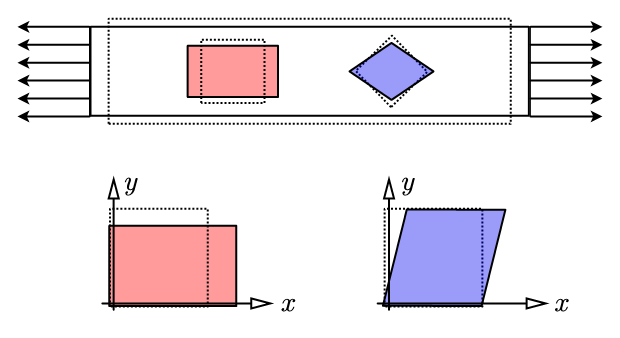
\includegraphics[width=7cm]{image/6-7-1.png}
\caption{正应变与剪应变}\label{6-7-1}
\end{wrapfigure}
其中三个对角元素$\varepsilon$称作\emph{正应变}(normal strain).\,而非对角的元素$\theta$称作\emph{剪应变}(shear strain).\,如图\ref{6-7-1}所示,\,在一种非常简单的模型中,\,大气中的棒被在沿棒方向施加一个拉力而伸长,\,但宽方向很自然地会产生些许的收缩.\,那么根据在棒里取出不同的微元形式,\,其变形方向也会有所改变.\,红色部分沿$x$方向就发生了明显的正应变.\,这是因为合适地平移,\,旋转其变形后的微元对齐形变前的微元(虚线)后,\,明显发现在$x$方向长度变大了.\,如果初始长度为$X$,\,之后在微元范围内端点的$x=X+\delta$.\,于是根据上面的定义,\,正应变其实就是:
\[\varepsilon=\frac{\delta}{X}=\frac{x-X}{X}\]

而蓝色部分是个平行四边形,\,将底边与变形前的底边对齐以后,\,我们发现$x-y$平面上顶角不再是$90^\circ$,\,这其实就标志着剪应变.\,如果这个角度减小了$\alpha$,\,那么之后的$x=X+Y\tan\alpha,\,y=Y$.\,这就说明$\delta_x=Y\tan\alpha,\,\delta_y=0$.\,从而:
\[\theta_{xy}=\frac{\partial \delta_y}{\partial X}+\frac{\partial \delta_x}{\partial Y}=\tan\alpha\approx \alpha\]

可见这个角度变化其实就是剪应变,\,它与边的对齐方式无关,\,如果$x,\,y$轴夹角变小便是正的.\,正应变,\,剪应变都是无量纲的物理量.

\vspace{0.5cm}

接下来需要考虑弹性体的内部受力情况.\,令人惊讶的是,\,它也必然由一个对称张量描述.\,首先我们意识到弹性力内部的受力具有以下特征:\,A.\,是空间点的函数,\,不同点处可以不同,\,但每一点应当有一个受力情况,\,它就是内部的\emph{应力}(stress).\,B.\,不是一个矢量.\,显然指出弹性体中的一点,\,并不能马上对应出来这个点处的某个受力的情况,\,因为我们考虑的是内力而不是外力,\,但是点处的受力不可能有明确的施力物体与受力物体.\,那么其实还需要在这一点处找到一个面矢量$\ud \bs{S}$,\,才能说是谁对谁的力.\,我们这样就发现了,\,其实指定一个应力,\,本质上就是在每一点指定一个面矢量$\ud \bs{S}$到相互作用力$\ud \bs{F}$的映射.\,C.\,显然,\,这样的映射应当为线性映射\footnote{证明留给读者做思考,\,需要用到极限微元受力分析.}.

\begin{wrapfigure}[15]{o}[-10pt]{7cm}
\vspace{-0.5cm}
\centering
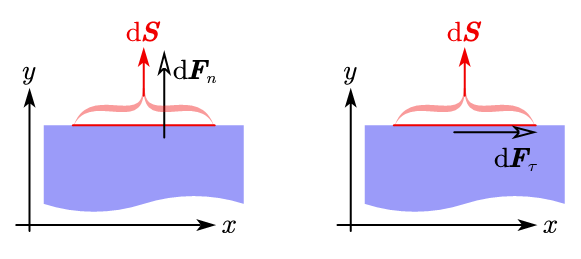
\includegraphics[width=7cm]{image/6-7-2.png}
\caption{正应力与剪应力}\label{6-7-2}
\end{wrapfigure}
这样就几乎已经说明,\,应力其实就是一个张量.\,因为从一个矢量$\ud \bs{S}$到另一个矢量$\ud \bs{F}$的线性映射的数学模型其实就是张量,\,它存在$3\times 3=9$个分量.\,我们进一步指定,\,$\ud \bs{F}$的含义$\ud \bs{S}$指向的那一侧的体元对这一侧的体元通过$\ud \bs{S}$施加的相互作用力.\,这个张量就是:
\[\left\{\begin{array}{ccc}\ud F_x &= & \sigma_{xx} \ud S_x + \sigma_{xy} \ud S_y+\sigma_{xz} \ud S_z \\ \ud F_y&= & \sigma_{yx} \ud S_x + \sigma_{yy} \ud S_y+\sigma_{yz} \ud S_z \\ \ud F_z &= & \sigma_{zx} \ud S_x + \sigma_{zy} \ud S_y+\sigma_{zz} \ud S_z \end{array}\right.\]
\[\bs{\sigma}:\; \ud \bs{S}\rightarrow \ud \bs{F}\]

\[\bs{\sigma}:\; \begin{bmatrix}\sigma_{xx}&\sigma_{xy}&\sigma_{xz}\\\sigma_{yx}&\sigma_{yy}&\sigma_{yz}\\\sigma_{zx}&\sigma_{zy}&\sigma_{zz}\end{bmatrix}\]

这个张量就叫做\emph{应力张量}(stress tensor).\,通过极限微元的受力分析,\,可以证明这个张量还必须是对称的\footnote{也留给读者自己完成.}.\,也就是说,\,我们可以写成以下形式:
\[\bs{\sigma}:\; \begin{bmatrix}\sigma_{x}&\tau_{xy}&\tau_{zx}\\\tau_{xy}&\sigma_{y}&\tau_{yz}\\\tau_{zx}&\tau_{yz}&\sigma_{z}\end{bmatrix}\]

同样的,\,参考图\ref{6-7-2},\,我们可以发现,\,对角线元素$\sigma$代表\emph{正应力}(normal stress)而非对角线元素$\tau$代表\emph{剪应变}(shear stress).\,如果把面元取为$\ud\bs{S}=\ud S_y\bs{e}_y$,\,考虑在平面上的受力就会产生两个分量:
\[\ud \bs{F}_n=\sigma_y \ud S_y\bs{e}_y\quad,\quad\ud \bs{F}_{\tau}=\tau_{xy} \ud S_y\bs{e}_x\]

前者就是垂直于面的以拉力为正的正应力,\,后者就是平行于面方向的剪应力.\,而应力本身都是和以往学过的压强量纲一致,\,国际单位是帕斯卡${\rm Pa}$:
\[\sigma=\frac{\ud F_n}{\ud S}\quad ,\quad \tau=\frac{\ud F_{\tau}}{\ud S}\]

\vspace{0.5cm}

引入两个张量以后,\,剩下的就是构造两者之间的因果关系:\,应力是如何造成应变的.\,在纯粹的弹性理论中,\,我们可以假设应力张量到应变张量的映射再一次是一个逐点线性的映射.\,这样的结果是数学上造成了每一点需要引入一个四阶的张量来描述这样的映射.\,三维情况下四阶的张量一共会造成$3^4=81$个独立分量.\,由于应力应变张量本身具有对称性,\,故其实只需要$6^2$个独立分量.\,再由于体系的非耗散性的要求\footnote{导致了某种形式互易定理.},\,其独立分量数最终减少到$21$个.\,这也是高度非对称的介质的弹性系数中独立的量的个数.\,然而,\,如果介质是完全各向同性的,\,也就是说沿所有三维空间中任意方向的长度与角度的拉伸与压缩都是相同困难的情况下,\,张量的对称性理论可以告诉我们,\,独立的弹性系数只会剩下两个.\,具体来说,\,$\bs{\varepsilon}$与$\bs{\sigma}$之间的关系必然会变成以下不依赖于坐标系选取的形式:
\[\bs{\sigma}=2\mu\cdot\bs{\varepsilon}+\lambda {\rm Tr}(\bs{\varepsilon})\cdot\bs{I}\]

而按照这样的方式选取的弹性系数$\lambda$和$\mu$被叫做\emph{拉梅参数}(Lam\'e parameters).\,式中${\rm Tr}$代表取迹操作,\,而$\bs{I}$是单位张量.\,带入之前的两个张量的写法上式实际上意味着:
\[\sigma_x=2\mu\varepsilon_x+\lambda(\varepsilon_x+\varepsilon_y+\varepsilon_z)\]
\[\sigma_y=2\mu\varepsilon_y+\lambda(\varepsilon_x+\varepsilon_y+\varepsilon_z)\]
\[\sigma_z=2\mu\varepsilon_z+\lambda(\varepsilon_x+\varepsilon_y+\varepsilon_z)\]
\[\tau_{ij}=\mu\theta_{ij}\]

至少我们能从上式发现,\,剪应力和正应力是分别独立地导致剪应变和正应变的,\,尤其是剪应力,\,它在三个方向甚至都是互相独立地,\,而这个比例系数就还被叫做\emph{剪变模量}(shear modulus),\,用$G$来表示.\,即拉梅系数$\mu\equiv G$.\,这个在切向成立的结论称作\emph{横向胡克定律}(transverse Hooke's law):
\[\frac{ F_\tau}{ S}=G \frac{ \delta}{ y}\]

而前三个式子对应的正应力正应变之间的关系比较复杂.\,首先我们把三式相加可以得到:
\[\sigma_x+\sigma_y+\sigma_z=(2\mu+3\lambda)(\varepsilon_x+\varepsilon_y+\varepsilon_z)\]\tabularnewline

我们意识到,\,任何物体在大气环境下实际上就受到周围分子不断撞击产生的大气压力而体积收缩,\,实际上就是三个方向应力相等于压强$\sigma_x=\sigma_y=\sigma_z=p$,\,而且三个应变$\varepsilon_i$就等价于线压缩率,\,应当是体压缩率的三分之一的情况,\,这样我们得到:
\[p=\left(\lambda+\frac{2}{3}\mu\right)\frac{\Delta V}{V}\]

这个系数就叫做\emph{体弹性模量}(bulk modulus):
\[K=\lambda+\frac{2}{3}\mu\]

一般来说,\,弹性体预先在大气体系中被压缩,\,在这个基础上,\,线性地叠加上由于其他形式的应力$\bs{\sigma}$导致的新应变$\bs{\varepsilon}$.\,

还有一种至关重要的变形.\,如果我们在一根弹性棒的$x$方向施加应力$\sigma$,\,但是$y-z$方向不施加任何的力$\sigma_y=\sigma_z=0$,\,扣除原来大气造成的应变,\,通过解方程得到$\varepsilon=\varepsilon_x$和$\varepsilon'=\varepsilon_y=\varepsilon_z$的值:
\[\left\{\begin{array}{ccc}\sigma &=&2\mu\varepsilon + \lambda(\varepsilon+2\varepsilon') \\ 0 &=&2\mu\varepsilon' + \lambda(\varepsilon+2\varepsilon')\end{array}\right.\Rightarrow\quad \left\{\begin{array}{ccc}\varepsilon &=& \frac{\lambda+\mu}{\mu(3\lambda+2\mu)} \sigma\\ \varepsilon' &=&-\frac{\lambda}{2(\lambda+\mu)}\varepsilon\end{array}\right.\]

第一个式子翻过来写就是描述拉力与棒伸长之间的\emph{纵向胡克定律}(longtitudinal Hooke's law).\,相关的弹性系数称作\emph{杨氏模量}(Young's modulus),\,即$E=\mu(3\lambda+2\mu)/(\lambda+\mu)$.\,而第二个式子反映了如果棒在拉力方向伸长,\,在垂直方向必然缩短的现实.\,缩短率与伸长率的比值称为\emph{泊松比}(Poisson's ratio),\,即$nu=\lambda/2(\lambda+\mu)$:
\[\frac{F_n}{S}=E\frac{\delta}{x}\quad ,\quad \frac{\delta'}{y}=\nu\frac{\delta}{x}\]

\begin{figure}[H]
\centering
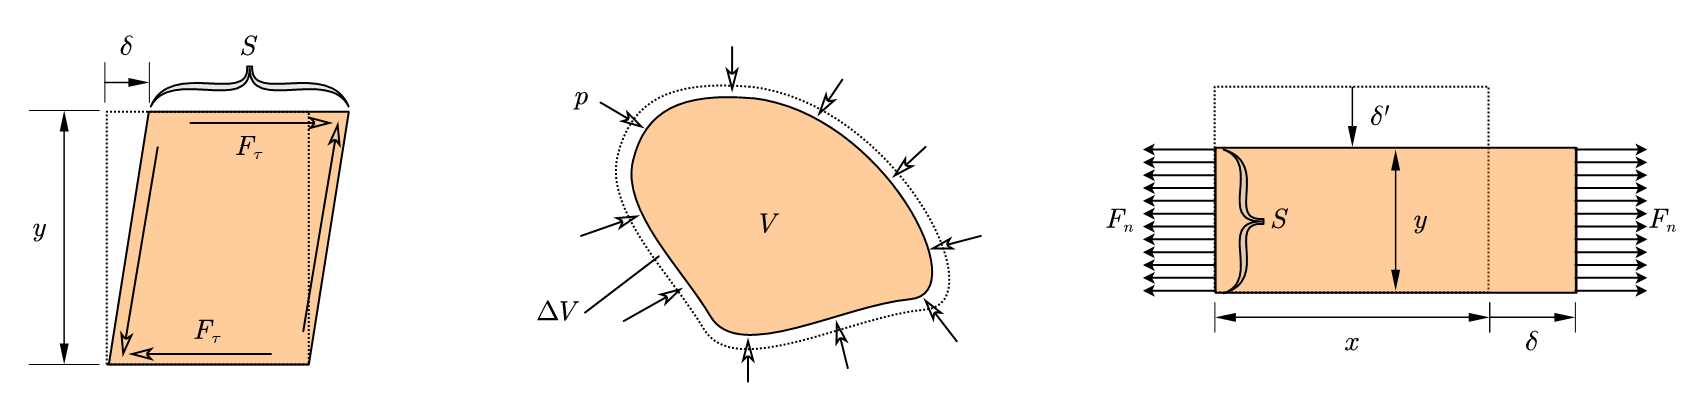
\includegraphics[width=14cm]{image/6-7-3.png}
\caption{剪变模量,\,体弹性模量与杨氏模量}
\end{figure}

三个弹性模量的单位也是应力的单位,\,即帕斯卡,\,而典型材料的弹性模量在$10^{10}{\rm Pa}$的数量级.


\section{弹性棒,\,弹性绳,\,弹性膜与弹性体}

\section{弹性波}


%%!TEX root = ../physical-olympics-2.tex
\chapter{相对论}


\section{相对论运动学}

\begin{itemize}
\item 光速不变原理:\,时空的结构为平直时空:\,$\text{d}s^2=c^2\text{d}t^2-\text{d}x_i^2$:\,物质运动的``舞台''.

\item 相对性原理:\,物理规律的协变性:
\[\text{Sca}.=\text{Sca}. \quad , \quad \text{Vec}.=\text{Vec}. \quad ,\quad  \text{Vec}.\cdot \text{Vec}.=\text{Sca}. \quad \text{etc}.\]

\item \emph{四-标量}(four-scalar)与\emph{四-矢量}(four-vector)的定义:\,类比三维空间标量矢量,\,但按闵可夫斯基空间处理.

\item 洛伦兹变换的定义:\,保度规的变换.\,物理上是不同共原点惯性参考者建立的参考系.

\item 洛伦兹群:
\[\text{SO}\left( 3,1 \right) =<R_x, R_y, R_z, B_x, B_y, B_z>\]

其中$B_x$为$x$方向的\emph{推促}(boost):
\[\left[ \begin{array}{c}
	ct\\
	x_1\\
	x_2\\
	x_3\\
\end{array} \right] ^{'} =\left[ \begin{matrix}
	\gamma&		-\gamma \beta&		0&		0\\
	-\gamma \beta&		\gamma&		0&		0\\
	0&		0&		1&		0\\
	0&		0&		0&		1\\
\end{matrix} \right] \left[ \begin{array}{c}
	ct\\
	x_1\\
	x_2\\
	x_3\\
\end{array} \right] \]

\item 经典物理没有协变性,\,但电磁学与相对论理论具有协变性.\,意为所有物理定律都由协变的对象构成,\,这主要包括标量,\,矢量,\,张量,\,旋量四类.\,四-矢量尤其常见:
\[\left[ \begin{array}{c}
	A_0\\
	A_1\\
	A_2\\
	A_3\\
\end{array} \right] ^{'} =\left[ \begin{matrix}
	\gamma&		-\gamma \beta&		0&		0\\
	-\gamma \beta&		\gamma&		0&		0\\
	0&		0&		1&		0\\
	0&		0&		0&		1\\
\end{matrix} \right] \left[ \begin{array}{c}
	A_0\\
	A_1\\
	A_2\\
	A_3\\
\end{array} \right] \]

出于方便,\,四-矢量也被简记为$A_{\mu}=\left( A_0, A_i \right) =\left( A_0, \boldsymbol{A} \right) $.\,而$A_i=\left( A_1, A_2, A_3 \right) $是三维矢量的简记.\,四-矢量与四-矢量可以算\emph{伪内积}(pseudo-inner-product):
\[A_{\mu}B^{\mu}=A_0B_0-A_iB_i\]

伪内积将得到四-标量.\,即参考系变换下不变的量.

\item 洛伦兹变换下任意四-矢量具有不变量$A_{\mu}A^{\mu}=A_{0}^{2}-\boldsymbol{A}^2$,\,对于类时四-矢量这将大于零,\,即$A_{\mu}A^{\mu}=A_{\text{proper}}^2$,\,事实上以速度$\boldsymbol{v}=\frac{\boldsymbol{A}}{A_0}c$做洛伦兹变换,\,可以把空间分量变为零.\,这叫做\emph{本征参考系}(proper reference system).\,得到本征四-矢量$A_{\mu}'=\left( A_{\text{proper}}, \mathbf{0} \right)$.

\item 三个基本图像:

\begin{itemize}
\item 尺缩:\,$L=L_0/\gamma$.

\item 钟慢:\,$t=\gamma t_0$.

\item 同时相对性:\,$\tau=-\beta \frac{x}{c}$.

\end{itemize}

只要是真的尺子,\,真的钟,\,就永远不可能错!\,没有真的尺子和钟就去构造.

\item 相对论质点运动:

具有四-标量:\,间隔$\text{d}s=\sqrt{\text{d}x_{\mu}\text{d}x^{\mu}}$,\,本征时$\ud t_0=\ud s/c$,\,下四-速度的不变模长$v_\mu v^\mu=c^2$.

具有四-矢量:\,四-位移$\text{d}x_{\mu}=\left( c\text{d}t, \text{d}\boldsymbol{r} \right) $,\,四-速度$v_{\mu}=\left( \gamma c, \gamma \boldsymbol{v} \right) $,\,四-加速度见下节.

\item 速度变换公式:

$$
\gamma '=\frac{1-\frac{uv_x}{c^2}}{\sqrt{1-u^2/c^2}}\gamma 
$$

$$
v_x'=\frac{v_x-u}{1-\frac{uv_x}{c^2}}
$$

$$
v_{y,z}'=\frac{\sqrt{1-u^2/c^2}}{1-\frac{uv_x}{c^2}}v_{y,z}
$$

\item 光行差公式:\,可以用速度变换推导,\,也可以之后用流变换推导:
\[\cos \theta'=\frac{\cos \theta -\beta}{1-\beta \cos\theta}\quad ,\quad \sin \theta'=\sin\theta\cdot \frac{\sqrt{1-\beta^2}}{1-\beta \cos\theta}\quad ,\quad \tan\theta =\frac{\sin \theta'}{\cos \theta'}\]

\item 相对论下讨论刚体?\,模型存在缺陷:\,隧道佯谬,\,转盘佯谬.\,故整个刚体运动学都没有必要建立.

\end{itemize}

\section{相对论动力学}

\begin{itemize}
\item 动量-能量构成四矢量的必要性:\,守恒律需要被保留且协变.

\item 四-动量:
\[p_{\mu}=\left( \frac{E}{c}, \boldsymbol{p} \right) \,\,, p_{\mu}p^{\mu}c^2=E^2-p^2c^2=m^2c^4\,\,, \boldsymbol{v}=\frac{\boldsymbol{p}c^2}{E}\]

\[\boldsymbol{p}=\frac{m\boldsymbol{v}}{\sqrt{1-v^2/c^2}}\,\,, E=\frac{mc^2}{\sqrt{1-v^2/c^2}}\]

\item 普遍的过程的守恒律:
\[\sum_i{p_{i,\mu}}=\sum_j{p_{j,\mu}}\]

\item 四-力与四-加速度:
\[a_{\mu}=\frac{\text{d}v_{\mu}}{\text{d}t_0}=\left( \gamma \frac{\text{d}\gamma}{\text{d}t}c, \gamma \frac{\text{d}\gamma \boldsymbol{v}}{\text{d}t} \right) \,\,, \frac{\text{d}\boldsymbol{v}}{\text{d}t}:=\boldsymbol{a}\]

\[F_{\mu}=\frac{\text{d}p_{\mu}}{\text{d}t_0}=\left( \gamma \frac{\text{d}E}{c\text{d}t},\gamma \frac{\text{d}\boldsymbol{p}}{\text{d}t} \right) :=\left( \gamma \frac{W}{c},\gamma \boldsymbol{F} \right) \]

\begin{itemize}
\item 推论一:\,$F_\mu=a_\mu$.\,但三维矢量之间不会直接符合Newton-like的动力学方程.

\item 推论而:\,$F_\mu v^\mu=0$.\,这个三维继续可以得到:
\[\boldsymbol{F}\text{d}t=\text{d}\boldsymbol{p}\,\,, \boldsymbol{F}\cdot \text{d}\boldsymbol{r}=\text{d}E\]
\end{itemize}

\item 单方向受力时,\,在该方向的推促下力不变.

\item 本征加速度与本征力:\,它本意指的是\emph{四-速度的本征系}中的四-加速度与四-力,\,不过神奇的是恰好让两者的时间分量变为零(类空,\,与类时的四-速度正交),\,空间分量为$\bs{a}_0,\,\bs{F}_0$:
\[\bs{F}_0=m\bs{a}_0\]
\[a_\mu a^\mu=-a_0^2\]

\item 沿平行于本征加速度与本征力方向施以推促:
\[F=F_0\quad ,\quad a=a_0/\gamma^3\]

\item 沿垂直于本征加速度与本征力方向施以推促:
\[F=F_0/\gamma\quad ,\quad a=a_0/\gamma^2\]

\item \emph{快度}(rapidity):\,$\beta={\rm th} \vartheta,\,\gamma={\rm ch} \vartheta$.

\item 自然坐标下的相对论性牛顿定律:
\[F_\tau=\gamma^3 ma_\tau\]
\[F_n=\gamma ma_n\]

\item 相对论关于碰撞的新理解:

\begin{table}[H]
\centering
\begin{tabular}{c|c|c}
\hline
情形 &经典 & 相对论\\\hline
弹性 & 无耗散,\,$\bs{p}'=\bs{p},\,E'=E$ &粒子守恒,\,$\bs{p}'=\bs{p},\,E'=E$\\\hline
非弹性 & 有耗散,\,$\bs{p}'=\bs{p},\,E$不可列 &粒子变性,\,$\bs{p}'=\bs{p},\,E'=E$\\\hline
\end{tabular}
\end{table}

只有一个例外:\,光子的散射若频率不变,\,叫做弹性散射.\,如经典的瑞利散射,\,米氏散射;\,但如果频率变了,\,叫做非弹性散射,\,如拉曼散射,\,康普顿散射.

\item 相对论碰撞根据具体情形一般有以下大的分类:\,弹性的散射,\,非弹性的散射,\,粒子反应.

\item 质点系的动量-能量也将构成一个四-矢量,\,即:
\[(E,\,\bs{p})=\sum_i (E_i,\,\bs{p}_i)\]

那么这个四-矢量的本征系速度:
\[\bs{v}=\frac{\bs{p}c^2}{E}\]

称作\emph{动量中心系}(center-of-momentum frame),\,以代替经典物理的质心系.\,简称动心系.\,顾名思义,\,此系中质点系总动量为零:\,而总能量:
\[E_0^2=E^2-\bs{p}^2c^2=m_0^2 c^4\]

$m_0$为动心系中的总动质量,\,以后称作质点系的等效静质量.\,这个式子可以解释一部分的质量起源问题.

\item 一个等效静质量$m_0$的质点系若选取相对动心系以$\bs{v}$运动的参考系,\,动量与能量为:
\[\bs{p}=\sum_i \bs{p}_i =\frac{m_0\boldsymbol{v}}{\sqrt{1-v^2/c^2}}\]
\[E=\sum_i E_i=\frac{m_0 c^2}{\sqrt{1-v^2/c^2}}\]

\item 放能反应:\,$\sum_i m_i>\sum_j m_j$.\,则无论取哪个系,\,静能转化为动能的量都相等.\,定义为反应能$Q$:
\[Q=\left(\sum_i m_i-\sum_j m_j\right)c^2\]

\item 吸能反应:\,$\sum_i m_i<\sum_j m_j$.\,则具有阈能.\,\emph{仅在动心系中},\,反应发生的最小动能(阈能)的值为:
\[Q=\left(\sum_j m_j-\sum_i m_i\right)c^2\]

\end{itemize}
	
\section{相对论连续物质}

\begin{itemize}
\item 若有一守恒荷$Q$作为四-标量,\,则其空间分布与流动构成一个密度场$\rho,\,\bs{j}$:
\[\ud Q=\rho\ud V\]
\[\ud Q=\bs{j}\cdot \ud \bs{S} \ud t\]

\item 那么$(\rho c,\,\bs{j})$是一个四-矢量且符合洛伦兹变换,\,如$x$方向的推促:
\[\left[ \begin{array}{c}
	\rho^{'}c\\
	j_x^{'}\\
	j_y^{'}\\
	j_z^{'}\\
\end{array} \right]  =\left[ \begin{matrix}
	\gamma&		-\gamma \beta&		0&		0\\
	-\gamma \beta&		\gamma&		0&		0\\
	0&		0&		1&		0\\
	0&		0&		0&		1\\
\end{matrix} \right] \left[ \begin{array}{c}
	\rho c\\
	j_x\\
	j_y\\
	j_z\\
\end{array} \right] \]

\item 若有一平面波场,\,其必要的一个要素为相位,\,它随着时空分布必然写作:
\[\varphi=\omega t-\bs{k}\cdot\bs{r}\]

$\omega$称作角频率,\,$\bs{k}$为波矢.

\item 那么由于相位为四-标量,\,且可以写作以下形式,\,故$k_\mu=(\omega/c,\,\bs{k})$为四-矢量,\,称作四-波矢:
\[\varphi=k_\mu x^\mu\]

如$x$方向的推促:
\[\left[ \begin{array}{c}
	\omega^{'}/c\\
	k_x^{'}\\
	k_y^{'}\\
	k_z^{'}\\
\end{array} \right]  =\left[ \begin{matrix}
	\gamma&		-\gamma \beta&		0&		0\\
	-\gamma \beta&		\gamma&		0&		0\\
	0&		0&		1&		0\\
	0&		0&		0&		1\\
\end{matrix} \right] \left[ \begin{array}{c}
	\omega /c\\
	k_x\\
	k_y\\
	k_z\\
\end{array} \right] \]

\item 可以从上式出发得到光行差公式,\,同时也能得到多普勒效应公式.\,在前提$\omega/k=c$(四-波矢类光)时:
\[\omega'=\omega\cdot \frac{1-\beta \cos\theta}{\sqrt{1-\beta^2}}\]

\[\cos \theta'=\frac{\cos \theta -\beta}{1-\beta \cos\theta}\]

\item 将三维的力密度和功率密度:
\[\bs{f}=\frac{\ud \bs{F}}{\ud V}\]
\[p=\frac{\ud P}{\ud V}\]

合并可以得到四-力密度$f_\mu=(p/c,\,\bs{f})$.

\end{itemize}

\section{相对论电磁场}

相对论场变换公式:
\[E_{//}'=E_{//}\quad ,\quad B_{//}'=B_{//}\]
\[\bs{E}_\perp'=\frac{\bs{E}_\perp+\bs{v}\times \bs{B}_\perp}{\sqrt{1-\beta^2}}\quad,\quad \bs{B}_\perp'=\frac{\bs{B}_\perp-\bs{v}\times \bs{E}_\perp/c^2}{\sqrt{1-\beta^2}}\]


\end{document}

%%%%%%%%%%%%%%%%%%%%%%%%%%%%%%%%%%%%%%%%%%%%%%%%%%%%%%%%%%%%%%%%%%%%%%%%%%%%%%